% Este documento tem a ver com as partes do LIVRO. 



% Tamanhos
% \tiny
% \scriptsize
% \footnotesize
% \small 
% \normalsize
% \large 
% \Large 
% \LARGE 
% \huge
% \Huge

% Posicionamento
% \centering 
% \raggedright
% \raggedleft
% \vfill 
% \hfill 
% \vspace{Xcm}   % Colocar * caso esteja no começo de uma página. Ex: \vspace*{...}
% \hspace{Xcm}

% Estilo de página
% \thispagestyle{<<nosso>>}
% \thispagestyle{empty}
% \thispagestyle{plain}  (só número, sem cabeço)
% https://www.overleaf.com/learn/latex/Headers_and_footers

% Compilador que permite usar fonte de sistema: xelatex, lualatex
% Compilador que não permite usar fonte de sistema: latex, pdflatex

% Definindo fontes
% \setmainfont{Times New Roman}  % Todo o texto
% \newfontfamily\avenir{Avenir}  % Contexto

\begingroup\thispagestyle{empty}\vspace*{.05\textheight}\parindent=0pt 
              \formular
              \Huge 
              \textbf{Liberdade}\smaller[1] 1880–1882        
              \bigskip

              \Large
              Luiz Gama
              \normalsize

			  \vfill\normalsize
              OBRAS COMPLETAS\hfill \textbf{volume} 8
     
\endgroup
\pagebreak       % [Frontistício]
\begingroup\footnotesize\parindent0pt\vspace*{3em}

\thispagestyle{empty}
{\formular\bfseries VOLUMES}\smallskip

1. Poesia, 1854–1865\\
2. Profecia, 1862–1864\\
3. Comédia, 1866–1867\\
4. Democracia, 1866–1869\\
5. Direito, 1870–1875\\
6. Crime, 1877–1879\\
7. Liberdade, 1880–1882\\
8. Justiça

\endgroup
\pagebreak
% Tamanhos
% \tiny
% \scriptsize
% \footnotesize
% \small 
% \normalsize
% \large 
% \Large 
% \LARGE 
% \huge
% \Huge

% Posicionamento
% \centering 
% \raggedright
% \raggedleft
% \vfill 
% \hfill 
% \vspace{Xcm}   % Colocar * caso esteja no começo de uma página. Ex: \vspace*{...}
% \hspace{Xcm}

% Estilo de página
% \thispagestyle{<<nosso>>}
% \thispagestyle{empty}
% \thispagestyle{plain}  (só número, sem cabeço)
% https://www.overleaf.com/learn/latex/Headers_and_footers

% Compilador que permite usar fonte de sistema: xelatex, lualatex
% Compilador que não permite usar fonte de sistema: latex, pdflatex

% Definindo fontes
% \setmainfont{Times New Roman}  % Todo o texto
% \newfontfamily\avenir{Avenir}  % Contexto

\begingroup\thispagestyle{empty}\vspace*{.05\textheight}\parindent=0pt 
              \formular
              \Huge 
              \textbf{Democracia}\smaller[1] 1866–1869        
              \bigskip

              \Large
              Luiz Gama
              \normalsize
              \vspace{3em}

              \small
              Bruno Lima (\textit{org.})
              \vspace{6em}

   					  1ª Edição
                      

              \vfill

              \newfontfamily\timesnewroman{Times New Roman}
              {\fontsize{30}{40}\selectfont \timesnewroman hedra}
              \smallskip

              \small
              São Paulo \the\year
\endgroup
\pagebreak
	       % [folha de rosto]
%\newcommand{\linhalayout}[2]{{\tiny\textbf{#1}\quad#2\par}}
\newcommand{\linha}[2]{\ifdef{#2}{\linhalayout{#1}{#2}}{}}

\begingroup\tiny
\parindent=0cm
\thispagestyle{empty}

\textbf{edição brasileira©}\quad			 {Hedra \the\year}\\
\textbf{organização©}\quad			 		 {Bruno Rodrigues de Lima}\\
\smallskip
%\textbf{agradecimentos}\quad			 	 {agradecimentos}\\

\textbf{edição}\quad			 			 {Jorge Sallum}\\
\textbf{coedição}\quad			 			 {Suzana Salama}\\
\textbf{assistência editorial}\quad			 {Paulo Pompermaier, \mbox{Ana Lancman}, \mbox{Sofia Boldrini}}\\
\textbf{revisão}\quad			 			 {Renier Silva}\\
\textbf{capa}\quad			 				 {Lucas Kroeff}\\
\smallskip

\textbf{ISBN}\quad			 				 {ISBN}\smallskip

\hspace{-5pt}\begin{tabular}{ll}
\textbf{conselho editorial} & Adriano Scatolin,  \\
							& Antonio Valverde,  \\
							& Caio Gagliardi,    \\
							& Jorge Sallum,      \\
							& Ricardo Valle,     \\
							& Tales Ab'Saber,    \\
							& Tâmis Parron      
\end{tabular}
 

\vfill

\textit{Grafia atualizada segundo o Acordo Ortográfico da Língua\\
Portuguesa de 1990, em vigor no Brasil desde 2009.}\\

\textit{Direitos reservados em língua\\ 
portuguesa somente para o Brasil}\\\smallskip

\textsc{editora hedra ltda.}\\
R.~Fradique Coutinho, 1139 (subsolo)\\
05416--011 São Paulo \textsc{sp} Brasil\\
Telefone/Fax +55 11 3097 8304\\\smallskip
editora@hedra.com.br\\
www.hedra.com.br\\
\bigskip
Foi feito o depósito legal.

\endgroup
\pagebreak
     % [Créditos]

% nothing			is level -3
% \book				is level -2
% \part				is level -1
% \chapter 			is level 0
% \section 			is level 1
% \subsection 		is level 2
% \subsubsection 	is level 3
% \paragraph 		is level 4
% \subparagraph 	is level 5
\setcounter{secnumdepth}{0}
\setcounter{tocdepth}{0}


% \renewcommand{\contentsname}{Índex} 	% Trocar nome do sumário para 'Índex'
\ifodd\thepage\relax\else\blankpage\fi 	% Verifica se página é par e coloca página branca
\tableofcontents*

%\book{\textsc{Testis nossis},  Mussum Ipsum}

\part{Amor é fogo que arde sem se ver}

\chapter{É um não querer mais que bem\footnote{Cacilds vidis litro abertis.} querer}

\newcommand{\pacote}[1]{\marginnote{\tiny\alltt{#1}}}


\pacote{edlab-extra}
\begin{epigraphs} 
\qitem{Cogitatio in vero exquirendo maxime versatur. 
		 Appetitus impellit ad agendum.}{\textsc{Marcus
		  Tullius Cicero}}
\end{epigraphs}

\pacote{lettrine.sty}
\lettrine[realheight]{\textcolor{red}{M}}{ussum Ipsum}, cacilds vidis litro abertis. Suco de cevadiss, é um leite
divinis, qui tem lupuliz, a\textcolor{green}{fi}matis, aguis e fermentis. Sapien in monti palavris
qui num significa nadis i pareci latim.  Diuretics paradis num copo é motivis
de denguis. Mauris nec dolor in eros commodo tempor. Aenean aliquam molestie
leo, vitae iaculis nisl. Ligue para \textcolor{green}{9-3129-4563}.


In elementis mé pra quem é amistosis quis leo. Vehicula non. Ut sed ex eros.
Vivamus sit amet nibh non tellus tristique interdum. Copo furadis é disculpa de
bebadis, arcu quam euismod magna. Todo mundo vê os porris que eu tomo, mas
ninguém vê os tombis que eu levo!

\section{É solitário andar por entre a gente}


Pra lá , depois divoltis porris, paradis. Praesent vel viverra nisi. Mauris
aliquet nunc non turpis scelerisque, eget. Nec orci ornare consequat. Praesent
lacinia ultrices\footnote{Praesent vel viverra nisi. Mauris
aliquet nunc non turpis scelerisque, eget.} consectetur.\footnote{Sed non ipsum.} Sed non ipsum felis. Si u mundo tá muito paradis?
Toma um mé que o mundo vai girarzis!\footnote{\textsc{Mussum}, Ipsum,
\textit{Cacilds vidis litro abertis}.}




Em pé sem cair, deitado sem dormir, sentado sem cochilar e fazendo pose. Quem
num gosta di mé, boa gentis num é. Não sou faixa preta cumpadi, sou preto
inteiris, inteiris. Aenean aliquam molestie leo, vitae iaculis nisl.

\settowidth{\versewidth}{Nay, nay, I leave thee not, thou goest too}
\begin{verse}[\versewidth]
\ldots \\*
His judgement rendered, he dissolved the Thing. \\*
\flagverse{Ingeborg} And your decision? \\*
\flagverse{Fridthjof} \vinphantom{And your decision?}
Have I ought to choose? \\*
Is not mine honour bound by his decree? \\*
And that I will redeem through Angantyr \\*
His paltry gold doth hide in Nastrand’s flood. \\*
Today will I depart. \\*
\flagverse{Ingeborg} \vinphantom{Today will I depart.}
And Ingeborg leave? \\*
\flagverse{Fridthjof} Nay, nay, I leave thee not,
thou goest too. \\*
\flagverse{Ingeborg} Impossible! \\*
\flagverse{Fridthjof} \vinphantom{Impossible!}
O! hear me, ere thou answerest.
\end{verse}

Interagi no mé, cursus quis, vehicula ac nisi. Admodum accumsan disputationi eu
sit. Vide electram sadipscing et per. Detraxit consequat et quo num tendi nada.
Atirei o pau no gatis, per gatis num morreus.

Suco de cevadiss deixa as pessoas mais interessantis. Tá deprimidis, eu conheço
uma cachacis que pode alegrar sua vidis. Praesent malesuada urna nisi, quis
volutpat erat hendrerit non. Nam vulputate dapibus. Quem manda na minha terra
sou euzis!

\subsection{É nunca contentar-se de contente}

Em pé sem cair, deitado sem dormir, sentado sem cochilar e fazendo pose. Quem
num gosta di mé, boa gentis num é. Não sou faixa preta cumpadi, sou preto
inteiris, inteiris. Aenean aliquam molestie leo, vitae iaculis nisl.

Interagi no mé, cursus quis, vehicula ac nisi. Admodum accumsan disputationi eu
sit. Vide electram sadipscing et per. Detraxit consequat et quo num tendi nada.
Atirei o pau no gatis, per gatis num morreus.

\pacote{alltt}
\begin{alltt}\normalfont			%Verso branco
I used to love my garden
But now my love is dead
   For I found a 
   			      		[ bachelor’s button
   In black-eyed 
              	        [ Susan’s bed.
\end{alltt}

Suco de cevadiss deixa as pessoas mais interessantis. Tá deprimidis, eu conheço
uma cachacis que pode alegrar sua vidis. Praesent malesuada urna nisi, quis
volutpat erat hendrerit non. Nam vulputate dapibus. Quem manda na minha terra
sou euzis!

\subsubsection{Posuere libero varius}

Mussum Ipsum, cacilds vidis litro abertis. Posuere libero varius. Nullam a nisl
ut ante blandit hendrerit. Aenean sit amet nisi. Mé faiz elementum girarzis,
nisi eros vermeio. Interessantiss quisso pudia ce receita de bolis, mais bolis
eu num gostis. Diuretics paradis num copo é motivis de denguis.

Per aumento de cachacis, eu reclamis. Todo mundo vê os porris que eu tomo, mas
ninguém vê os tombis que eu levo! Admodum accumsan disputationi eu sit. Vide
electram sadipscing et per. Detraxit consequat et quo num tendi nada.

\chapter{Leite de capivaris, leite de mula manquis sem cabeça}

Leite de capivaris, leite de mula manquis sem cabeça. Suco de cevadiss deixa as
pessoas mais interessantis. Casamentiss faiz malandris se pirulitá. Em pé sem
cair, deitado sem dormir, sentado sem cochilar e fazendo pose.

Praesent vel viverra nisi. Mauris aliquet nunc non turpis scelerisque, eget.
Atirei o pau no gatis, per gatis num morreus. Quem num gosta di mé, boa gentis
num é. Paisis, filhis, espiritis santis.

\settowidth{\versewidth}{É solitário andar por entre a gente;}\label{camoes}
\begin{verse}[\versewidth]
\linenumbers

Amor é fogo que arde sem se ver;\\*
É ferida que dói e não se sente;\\*
É um contentamento descontente;\\*
É dor que desatina sem doer;\\!

É um não querer mais que bem querer;\\*
É solitário andar por entre a gente;\\*
É nunca contentar-se de contente;\\*
É cuidar que se ganha em se perder;\\!

É querer estar preso por vontade;\\*
É servir a quem vence, o vencedor;\\*
É ter com quem nos mata lealdade.\\!

Mas como causar pode seu favor\\*
Nos corações humanos amizade,\\*
Se tão contrário a si é o mesmo Amor?\\!

                 \hfill    \textsc{Luís de Camões}
\end{verse}

\marginnote{\footnotesize \textcolor{green}{Pra lá, depois divoltis porris, paradis. Praesent vel viverra nisi.}}
Delegadis gente finis, bibendum egestas augue arcu ut est. Praesent malesuada
urna nisi, quis volutpat erat hendrerit non. Nam vulputate dapibus. Nullam
volutpat risus nec leo commodo, ut interdum diam laoreet. Sed non consequat
odio. Si num tem leite então bota uma pinga aí cumpadi!

Sapien in monti palavris qui num significa nadis i pareci latim.  Quem num
gosta di mim que vai caçá sua turmis! A ordem dos tratores não altera o pão
duris. Quem manda na minha terra sou euzis!

Não sou faixa preta cumpadi, sou preto inteiris, inteiris. Manduma pindureta
quium dia nois paga. Aenean aliquam molestie leo, vitae iaculis nisl. Si u
mundo tá muito paradis? Toma um mé que o mundo vai girarzis!

Viva Forevis aptent taciti sociosqu ad litora torquent. Cevadis im ampola pa
arma uma pindureta. In elementis mé pra quem é amistosis quis leo. Nec orci
ornare consequat. Praesent lacinia ultrices consectetur. Sed non ipsum felis.
%


%h	Place the float here, i.e., 
% 	   approximately at the same point it 
% 	   occurs in the source text (however, not exactly at the spot)
%t	Position at the top of the page.
%b	Position at the bottom of the page.
%p	Put on a special page for floats only.
%!	Override internal parameters LATEX uses for determining "good" float positions.
%H	Places the float at precisely the location in the LATEX code. 
%	  Requires the float package (\usepackage{float}). This is 
%	  somewhat equivalent to h!, though some errors may 
%	  arise if you have too many consecutive floats with [H].
%   LINK: https://www.overleaf.com/learn/latex/Positioning_of_Figures

\pacote{graphicx}
\begin{figure}[h]
\centering
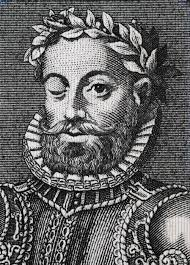
\includegraphics[width=0.5\textwidth]{image}
\caption{Camões Caolhiuos}
\label{fig:camoes}
\end{figure}

Interagi no mé, cursus quis, vehicula ac nisi. Mauris nec dolor in eros commodo
tempor. Aenean aliquam molestie leo, vitae iaculis nisl. Suco de cevadiss, é um
leite divinis, qui tem lupuliz, matis, aguis e fermentis. Copo furadis é
disculpa de bebadis, arcu quam euismod magna.



\paragraph{É cuidar que se ganha em se perder}

Mussum Ipsum, cacilds vidis litro abertis. Mais vale um bebadis conhecidiss,
que um alcoolatra anonimis. Per aumento de cachacis, eu reclamis. Si num tem
leite então bota uma pinga aí cumpadi! Cevadis im ampola pa arma uma pindureta.\footnote{Ver poema na 
		seção \ref{camoes} (p.\,\pageref{camoes}) e também 
		% LINK https://www.overleaf.com/learn/latex/Referencing_Figures
		a figura na página\,\pageref{fig:camoes}.
		\label{notasobrecamoes}}


\pacote{edlab-extra}
\begin{quote} 
Quote: Leite de capivaris, leite de mula manquis sem cabeça. Suco de
cevadiss deixa as pessoas mais interessantis. Casamentiss faiz malandris se
pirulitá. Em pé sem cair, deitado sem dormir, sentado sem cochilar e fazendo
pose.  
\end{quote}

Suco de cevadiss deixa as pessoas mais interessantis. Manduma pindureta quium
dia nois paga. Nec orci ornare consequat. Praesent lacinia ultrices
consectetur. Sed non ipsum felis. Posuere libero varius. Nullam a nisl ut ante
blandit hendrerit. Aenean sit amet nisi.

Vehicula non. Ut sed ex eros. Vivamus sit amet nibh non tellus tristique
interdum. Copo furadis é disculpa de bebadis, arcu quam euismod magna. Mé faiz
elementum girarzis, nisi eros vermeio. Admodum accumsan disputationi eu sit.
Vide electram sadipscing et per.

Casamentiss faiz malandris se pirulitá. Aenean aliquam molestie leo, vitae
iaculis nisl. Paisis, filhis, espiritis santis. Tá deprimidis, eu conheço uma
cachacis que pode alegrar sua vidis.

Suco de cevadiss, é um leite divinis, qui tem lupuliz, matis, aguis e
fermentis. Quem manda na minha terra sou euzis! Quem num gosta di mé, boa
gentis num é. Pra lá , depois divoltis porris, paradis.

A ordem dos tratores não altera o pão duris. Em pé sem cair, deitado sem
dormir, sentado sem cochilar e fazendo pose. Delegadis gente finis, bibendum
egestas augue arcu ut est. Detraxit consequat e
t quo num tendi nada.\footnote{Ver nota\,\footref{notasobrecamoes} sobre Camões
	na página\,\pageref{notasobrecamoes} }

Praesent vel viverra nisi. Mauris aliquet nunc non turpis scelerisque, eget. In
elementis mé pra quem é amistosis quis leo. Não sou faixa preta cumpadi, sou
preto inteiris, inteiris. Interessantiss quisso pudia ce receita de bolis, mais
bolis eu num gostis.

Atirei o pau no gatis, per gatis num morreus. Praesent malesuada urna nisi,
quis volutpat erat hendrerit non. Nam vulputate dapibus. Quem num gosta di mim
que vai caçá sua turmis! Viva Forevis aptent taciti sociosqu ad litora
torquent.

Nullam volutpat risus nec leo commodo, ut interdum diam laoreet. Sed non
consequat odio. Interagi no mé, cursus quis, vehicula ac nisi. Leite de
capivaris, leite de mula manquis sem cabeça. Sapien in monti palavris qui num
significa nadis i pareci latim.

Diuretics paradis num copo é motivis de denguis. Mauris nec dolor in eros
commodo tempor. Aenean aliquam molestie leo, vitae iaculis nisl. Si u mundo tá
muito paradis? Toma um mé que o mundo vai girarzis! Todo mundo vê os porris que
eu tomo, mas ninguém vê os tombis que eu levo!

Interagi no mé, cursus quis, vehicula ac nisi. Viva Forevis aptent taciti
sociosqu ad litora torquent. Quem manda na minha terra sou euzis! Praesent vel
viverra nisi. Mauris aliquet nunc non turpis scelerisque, eget.

Si u mundo tá muito paradis? Toma um mé que o mundo vai girarzis! Atirei o pau
no gatis, per gatis num morreus. Quem num gosta di mé, boa gentis num é. A
ordem dos tratores não altera o pão duris.

Delegadis gente finis, bibendum egestas augue arcu ut est. Mauris nec dolor in
eros commodo tempor. Aenean aliquam molestie leo, vitae iaculis nisl. Mais vale
um bebadis conhecidiss, que um alcoolatra anonimis. Em pé sem cair, deitado sem
dormir, sentado sem cochilar e fazendo pose.

\subparagraph{É querer estar preso por vontade}

Atirei o pau no gatis, per gatis num morreus. Praesent malesuada urna nisi,
quis volutpat erat hendrerit non. Nam vulputate dapibus. Quem num gosta di mim
que vai caçá sua turmis! Viva Forevis aptent taciti sociosqu ad litora
torquent.

Nullam volutpat risus nec leo commodo, ut interdum diam laoreet. Sed non
consequat odio. Interagi no mé, cursus quis, vehicula ac nisi. Leite de
capivaris, leite de mula manquis sem cabeça. Sapien in monti palavris qui num
significa nadis i pareci latim.


Nullam volutpat risus nec leo commodo, ut interdum diam laoreet. Sed non
consequat odio. Interagi no mé, cursus quis, vehicula ac nisi. Leite de
capivaris, leite de mula manquis sem cabeça. Sapien in monti palavris qui num
significa nadis i pareci latim.

Diuretics paradis num copo é motivis de denguis. Mauris nec dolor in eros
commodo tempor. Aenean aliquam molestie leo, vitae iaculis nisl. Si u mundo tá
muito paradis? Toma um mé que o mundo vai girarzis! Todo mundo vê os porris que
eu tomo, mas ninguém vê os tombis que eu levo!

Interagi no mé, cursus quis, vehicula ac nisi. Viva Forevis aptent taciti
sociosqu ad litora torquent. Quem manda na minha terra sou euzis! Praesent vel
viverra nisi. Mauris aliquet nunc non turpis scelerisque, eget.

Si u mundo tá muito paradis? Toma um mé que o mundo vai girarzis! Atirei o pau
no gatis, per gatis num morreus. Quem num gosta di mé, boa gentis num é. A
ordem dos tratores não altera o pão duris.

Delegadis gente finis, bibendum egestas augue arcu ut est. Mauris nec dolor in
eros commodo tempor. Aenean aliquam molestie leo, vitae iaculis nisl. Mais vale
um bebadis conhecidiss, que um alcoolatra anonimis. Em pé sem cair, deitado sem
dormir, sentado sem cochilar e fazendo pose.

\subparagraph{É querer estar preso por vontade}

Atirei o pau no gatis, per gatis num morreus. Praesent malesuada urna nisi,
quis volutpat erat hendrerit non. Nam vulputate dapibus. Quem num gosta di mim
que vai caçá sua turmis! Viva Forevis aptent taciti sociosqu ad litora
torquent.

Nullam volutpat risus nec leo commodo, ut interdum diam laoreet. Sed non
consequat odio. Interagi no mé, cursus quis, vehicula ac nisi. Leite de
capivaris, leite de mula manquis sem cabeça. Sapien in monti palavris qui num
significa nadis i pareci latim.


Nullam volutpat risus nec leo commodo, ut interdum diam laoreet. Sed non
consequat odio. Interagi no mé, cursus quis, vehicula ac nisi. Leite de
capivaris, leite de mula manquis sem cabeça. Sapien in monti palavris qui num
significa nadis i pareci latim.

Diuretics paradis num copo é motivis de denguis. Mauris nec dolor in eros
commodo tempor. Aenean aliquam molestie leo, vitae iaculis nisl. Si u mundo tá
muito paradis? Toma um mé que o mundo vai girarzis! Todo mundo vê os porris que
eu tomo, mas ninguém vê os tombis que eu levo!

Interagi no mé, cursus quis, vehicula ac nisi. Viva Forevis aptent taciti
sociosqu ad litora torquent. Quem manda na minha terra sou euzis! Praesent vel
viverra nisi. Mauris aliquet nunc non turpis scelerisque, eget.

Si u mundo tá muito paradis? Toma um mé que o mundo vai girarzis! Atirei o pau
no gatis, per gatis num morreus. Quem num gosta di mé, boa gentis num é. A
ordem dos tratores não altera o pão duris.

Delegadis gente finis, bibendum egestas augue arcu ut est. Mauris nec dolor in
eros commodo tempor. Aenean aliquam molestie leo, vitae iaculis nisl. Mais vale
um bebadis conhecidiss, que um alcoolatra anonimis. Em pé sem cair, deitado sem
dormir, sentado sem cochilar e fazendo pose.

\subparagraph{É querer estar preso por vontade}

Atirei o pau no gatis, per gatis num morreus. Praesent malesuada urna nisi,
quis volutpat erat hendrerit non. Nam vulputate dapibus. Quem num gosta di mim
que vai caçá sua turmis! Viva Forevis aptent taciti sociosqu ad litora
torquent.

Nullam volutpat risus nec leo commodo, ut interdum diam laoreet. Sed non
consequat odio. Interagi no mé, cursus quis, vehicula ac nisi. Leite de
capivaris, leite de mula manquis sem cabeça. Sapien in monti palavris qui num
significa nadis i pareci latim.


Nullam volutpat risus nec leo commodo, ut interdum diam laoreet. Sed non
consequat odio. Interagi no mé, cursus quis, vehicula ac nisi. Leite de
capivaris, leite de mula manquis sem cabeça. Sapien in monti palavris qui num
significa nadis i pareci latim.

Diuretics paradis num copo é motivis de denguis. Mauris nec dolor in eros
commodo tempor. Aenean aliquam molestie leo, vitae iaculis nisl. Si u mundo tá
muito paradis? Toma um mé que o mundo vai girarzis! Todo mundo vê os porris que
eu tomo, mas ninguém vê os tombis que eu levo!

Interagi no mé, cursus quis, vehicula ac nisi. Viva Forevis aptent taciti
sociosqu ad litora torquent. Quem manda na minha terra sou euzis! Praesent vel
viverra nisi. Mauris aliquet nunc non turpis scelerisque, eget.

Si u mundo tá muito paradis? Toma um mé que o mundo vai girarzis! Atirei o pau
no gatis, per gatis num morreus. Quem num gosta di mé, boa gentis num é. A
ordem dos tratores não altera o pão duris.

Delegadis gente finis, bibendum egestas augue arcu ut est. Mauris nec dolor in
eros commodo tempor. Aenean aliquam molestie leo, vitae iaculis nisl. Mais vale
um bebadis conhecidiss, que um alcoolatra anonimis. Em pé sem cair, deitado sem
dormir, sentado sem cochilar e fazendo pose.

\subparagraph{É querer estar preso por vontade}

Atirei o pau no gatis, per gatis num morreus. Praesent malesuada urna nisi,
quis volutpat erat hendrerit non. Nam vulputate dapibus. Quem num gosta di mim
que vai caçá sua turmis! Viva Forevis aptent taciti sociosqu ad litora
torquent.

Nullam volutpat risus nec leo commodo, ut interdum diam laoreet. Sed non
consequat odio. Interagi no mé, cursus quis, vehicula ac nisi. Leite de
capivaris, leite de mula manquis sem cabeça. Sapien in monti palavris qui num
significa nadis i pareci latim.

 %\textbf{SUMÁRIO}
%
%As Obras Completas de Luiz Gama
%
%Agradecimentos
%
%Nota sobre o estabelecimento do texto
%
%Cronologia
%
%Introdução ao Volume VII
%
%\textbf{UMA AUTOBIOGRAFIA}
%
%\textbf{1.} \emph{Bilhete para Lucio de Mendonça}
%
%Missiva Particular, São Paulo, 25 de Julho de 1880
%
%\textbf{1. 1.} \emph{Carta a Lucio de Mendonça}
%
%Missiva Particular, São Paulo, 25 de Julho de 1880
%
%\textbf{1. 2.} \emph{Minha Mãe}
%
%Missiva Particular, São Paulo, 1861 ca.
%
%\textbf{1. 3.} \emph{Luiz Gama por Lucio de Mendonça}
%
%Gazeta da Tarde, Rio de Janeiro, 15 de Dezembro de 1880
%
%\textbf{TRÊS SPARTACUS E UM JOHN BROWN}
%
%\textbf{2.} \emph{Aos homens da ordem}
%
%Gazeta do Povo, São Paulo, 1880
%
%\textbf{3.} \emph{A questão de raças}
%
%Gazeta do Povo, São Paulo, 18 de Julho de 1880
%
%\textbf{4.} \emph{À s. excia. o ilmo. sr. dr. chefe de polícia}
%
%Gazeta de S. Paulo, São Paulo, 02 de Junho de 1881
%
%\textbf{5.} \emph{Ao exmo. sr. conselheiro presidente do Tribunal da
%Relação}
%
%Gazeta de S. Paulo, São Paulo, 11 de Janeiro de 1881
%
%\textbf{A LUTA PELO DIREITO}
%
%\textbf{O TÚMULO DA CONSTITUIÇÃO}
%
%\textbf{6.} \emph{A lei e os ``cafetões''}
%
%A Província de S. Paulo, São Paulo, 1880
%
%\textbf{7.} \emph{O exmo. sr. dr. chefe de polícia}
%
%A Província de S. Paulo, São Paulo, 1880
%
%\textbf{8.} \emph{A deportação dos ``cafetões''}
%
%A Província de S. Paulo, São Paulo, 1880
%
%\textbf{9.} \emph{{[}A deportação dos ``cafetões'' -- II{]}
%Habeas-Corpus}
%
%A Província de S. Paulo, São Paulo, 1880
%
%\textbf{A PELEJA DO ADVOGADO CONTRA O BACHAREL}
%
%\textbf{10.} \emph{Luiz Gama ao público}
%
%Gazeta do Povo, São Paulo, 25 de Setembro de 1880
%
%\textbf{10. 1.} \emph{Luiz Gama ao público {[}réplica{]}}
%
%Gazeta do Povo, São Paulo, 26 de Setembro de 1880
%
%\textbf{11.} \emph{Insânia e calúnia}
%
%Gazeta do Povo, São Paulo, 03 de Outubro de 1880
%
%\textbf{FONTES DO DIREITO E ESTRATÉGIAS DE LIBERDADE}
%
%\textbf{12.} \emph{Questão forense}
%
%A Província de S. Paulo, São Paulo, 14 de Outubro de 1880
%
%\textbf{13.} \emph{Fato grave -- Jaú}
%
%A Província de S. Paulo, São Paulo, 20 de Outubro de 1880
%
%\textbf{14.} \emph{Aresto notável}
%
%A Província de S.Paulo, São Paulo, 17 de Novembro de 1880
%
%\textbf{15.} \emph{2ª Vara Cível}
%
%A Província de S.Paulo, São Paulo, 28 de Novembro de 1880
%
%\textbf{16.} \emph{Questão Jurídica {[}I{]}}
%
%A Província de S. Paulo, São Paulo, 18 de Dezembro de 1880
%
%\textbf{17.} \emph{Libertação de escravos pelo fundo de emancipação}
%
%A Província de S. Paulo, São Paulo, 21 de Dezembro de 1880
%
%\textbf{18.} \emph{Contraprotesto}
%
%A Província de S. Paulo, São Paulo, 4 de Janeiro de 1881
%
%\textbf{19.} \emph{Questão jurídica {[}II{]}}
%
%Gazeta de S. Paulo, São Paulo, 13 de Janeiro de 1881
%
%\textbf{O COCHEIRO E O CÔNSUL}
%
%\textbf{20.} \emph{Processo Vira-Mundo }
%
%Gazeta do Povo, São Paulo, 23 de Abril de 1881
%
%\textbf{21.} \emph{{[}Resposta ao sr. F...{]}}
%
%A Província de S. Paulo, São Paulo, 17 de Março de 1881
%
%\textbf{22.} \emph{A colônia portuguesa }
%
%Gazeta do Povo, São Paulo, 21 de Maio de 1881
%
%\textbf{UMA ESTÁTUA, UM COVEIRO E UM PERITO CRIMINAL}
%
%\textbf{23.} \emph{É de admirar}
%
%A Província de S. Paulo, São Paulo, 23 de Novembro de 1880
%
%\textbf{24.} \emph{Despertador Moral --- I}
%
%A Província de S. Paulo, São Paulo, 24 de Novembro de 1880
%
%\textbf{25.} \emph{Despertador Moral --- II}
%
%A Província de S. Paulo, São Paulo, 25 de Novembro de 1880
%
%\textbf{26.} \emph{Despertador Moral --- III}
%
%A Província de S. Paulo, São Paulo, 27 de Novembro de 1880
%
%\textbf{27.} \emph{Despertador Moral --- IV}
%
%A Província de S. Paulo, São Paulo, 1º de Dezembro de 1880
%
%\textbf{UM CRIME PUXA OUTRO}
%
%\textbf{28.} \emph{Exemplo de piedade, I}
%
%Gazeta de S. Paulo, São Paulo, 5 de Fevereiro de 1881
%
%\textbf{28. 1.} \emph{{[}Réplica do misericordioso Almeida{]}}
%
%Gazeta de S. Paulo, São Paulo, 5 de Fevereiro de 1881
%
%\textbf{29.} \emph{Máscara caída}
%
%Gazeta de S. Paulo, São Paulo, 6 de Fevereiro de 1881
%
%\textbf{30.} \emph{Como se conta a história}
%
%Gazeta de S. Paulo, São Paulo, 7 de Fevereiro de 1881
%
%\textbf{31.} \emph{O crime da rua de S. Bento }
%
%A Província de S. Paulo, São Paulo, 6 de Fevereiro de 1881
%
%\textbf{31. 1.} \emph{O promotor ao público da capital e o crime da rua
%de S. Bento {[}réplica{]} }
%
%A Província de S. Paulo, São Paulo, 7 de Fevereiro de 1881
%
%\textbf{O ÁS DA ABOLIÇÃO: A CARTA DE LUIZ GAMA PARA FERREIRA DE MENEZES}
%
%\textbf{32.} \emph{Trechos de uma carta}
%
%Gazeta da Tarde, Rio de Janeiro, 1º de Dezembro de 1880
%
%\textbf{33.} \emph{Trechos de uma carta}
%
%Gazeta da Tarde, Rio de Janeiro, 12 de Dezembro de 1880
%
%\textbf{34.} \emph{Carta ao dr. Ferreira de Menezes}
%
%Gazeta da Tarde, Rio de Janeiro, 16 de Dezembro de 1880
%
%\textbf{35.} \emph{Trechos de uma carta}
%
%Gazeta da Tarde, Rio de Janeiro, 28 de Dezembro de 1880
%
%\textbf{36.} \emph{Trechos de uma carta}
%
%Gazeta da Tarde, Rio de Janeiro, 1º de Janeiro de 1881
%
%\textbf{37.} \emph{Carta ao dr. Ferreira de Menezes}
%
%Gazeta da Tarde, Rio de Janeiro, 4 de Janeiro de 1881
%
%\textbf{38.} \emph{Carta ao dr. Ferreira de Menezes}
%
%Gazeta da Tarde, Rio de Janeiro, 7 de Janeiro de 1881
%
%\textbf{39.} \emph{Carta ao dr. Ferreira de Menezes}
%
%Gazeta da Tarde, Rio de Janeiro, 22 de Janeiro de 1881
%
%\textbf{40.} \emph{Carta ao dr. Ferreira de Menezes}
%
%Gazeta da Tarde, Rio de Janeiro, 23 de Janeiro de 1881
%
%\textbf{41.} \emph{Carta ao dr. Ferreira de Menezes}
%
%Gazeta da Tarde, Rio de Janeiro, 29 de Janeiro de 1881
%
%\textbf{42.} \emph{Carta ao dr. Ferreira de Menezes}
%
%Gazeta da Tarde, Rio de Janeiro, 1º de Fevereiro de 1881
%
%\textbf{A EMANCIPAÇÃO AO PÉ DA LETRA}
%
%\textbf{43.} \emph{Emancipação {[}I{]}}
%
%A Província de S. Paulo, São Paulo, 1º de Dezembro de 1880
%
%\textbf{44.} \emph{{[}Emancipação -- II{]} À redação da ``Província''}
%
%A Província de S. Paulo, São Paulo, 4 de Dezembro de 1880
%
%\textbf{45.} \emph{Emancipação {[}III{]}}
%
%A Província de S. Paulo, São Paulo, 15 de Dezembro de 1880
%
%\textbf{46.} \emph{A emancipação ao pé da letra {[}IV{]}}
%
%Gazeta do Povo, São Paulo, 18 de Dezembro de 1880
%
%\textbf{A DEFESA DA CARTA A FERREIRA DE MENEZES}
%
%\textbf{47.} \emph{Limeira ---} \emph{Ao sr. Luiz Gama {[}réplica{]}}
%
%A Província de S. Paulo, São Paulo, 21 de Dezembro de 1880
%
%\textbf{47. 1.} \emph{Reparação devida}
%
%A Província de S. Paulo, São Paulo, 21 de Dezembro de 1880
%
%\textbf{48.} \emph{O exmo. sr. comendador J. A. Paula Machado}
%
%A Província de S. Paulo, São Paulo, 12 de Janeiro de 1881
%
%\textbf{49.} \emph{Retificação necessária}
%
%Gazeta de S. Paulo, São Paulo, 14 de Janeiro de 1881
%
%\textbf{CRUELDADE NO QUARTEL}
%
%\textbf{50.} \emph{Ao Governo --- É grave {[}I{]}}
%
%Gazeta de S. Paulo, São Paulo, 15 de Janeiro de 1881
%
%\textbf{50. 1.} \emph{Ao Governo --- É grave {[}réplica{]}}
%
%Gazeta de S. Paulo, São Paulo, 16 de Janeiro de 1881
%
%\textbf{51.} \emph{Ao Governo --- É grave {[}II{]}}
%
%Gazeta de S. Paulo, São Paulo, 17 de Janeiro de 1881
%
%\textbf{52.} \emph{Ao honrado sr. dr. presidente da Província}
%
%Gazeta de S. Paulo, São Paulo, 21 de Janeiro de 1881
%
%\textbf{53.} \emph{Aos paulistas}
%
%Gazeta de S. Paulo, São Paulo, 21 de Janeiro de 1881
%
%\textbf{AGONIZA, MAS NÃO MORRE}
%
%\textbf{54.} \emph{Meu nobre amigo }
%
%Gazeta da Tarde, São Paulo, 21 de Julho de 1881
%
%\textbf{53.} \emph{O digno sr. dr. Guilherme Caetano da Silva}
%
%Correio Paulistano, São Paulo, 04 de Novembro de 1881
%
%\textbf{54.} \emph{Carta a José Maria Lisboa}
%
%Missiva particular, São Paulo, s.d., 1881
%
%\textbf{55.} \emph{À forca o Cristo da multidão}
%
%O Tiradentes, Rio de Janeiro, 21 de Abril de 1882
%
%\textbf{56.} \emph{Carta ao dr. Cerqueira César }
%
%Gazeta da Tarde, Rio de Janeiro, 17 de Junho de 1882
%
%\textbf{57.} \emph{Uma representação ao imperador d. Pedro II }
%
%Gazeta da Tarde, Rio de Janeiro, 08 de Agosto de 1882
%
%***
%
%Abreviações e siglas
%
%Cronologia
%
%Glossário mitológico, histórico e geográfico
%
%Glossário de verbetes
%
%Indíce biográfico
%
%Índice de referências multinormativas
%
%Índice remissivo

\part{Uma autobiografia}

\begin{didas}
\emph{A carta de Luiz Gama a Lucio de Mendonça e a transformação dela,
por Mendonça, em um perfil biográfico, que imediatamente foi publicado
na imprensa, constituem essa seção. A disposição textual, portanto,
segue o conhecido roteiro dessa correspondência histórica: a carta de
Gama, antecipada por um bilhete e acrescida de um poema, e a resposta,
agora pública, de Mendonça. Há muitas nuances para se debater sobre o
conteúdo da famosa carta, entre elas, a razão que levou Gama a escolher
Mendonça como portador da mensagem que se revelaria fantástica e, sob
todos os aspectos, digna das melhores páginas da história do Brasil. No
entanto, deixemos debates que poderiam descambar para pormenores
acadêmicos para outra ocasião. Procuremos aqui, num exercício de
criatividade e imaginação, ler a carta como se fossemos nós mesmos os
destinatários dela. Assim, a dimensão privada da missiva -- desfeita
após cinquenta anos do endereçamento original! -- perde fôlego e resta o
que o narrador brilhante talvez intentasse lá atrás, vislumbrando quiçá
a perenidade do texto: a escrita autobriográfica da experiência de vida,
tempos, angústias, sonhos, frustrações, provações, dilemas, conquistas e
lutas, o sofrimento em suma de um autor. Em síntese: embora tecnicamente
uma correspondência particular, a carta -- enigmática, cifrada e
luminosa feito "trovão dentro da mata" -- pode ter sido concebida (e não
duvidaríamos nós da genialidade de um mestre da literatura) para ganhar,
com o tempo, a dimensão autobiográfica que possui quando o leitor se
permite receber a carta como real destinatário dela. O pacto
escritor-leitor, portanto, ganha novo e original sentido. Tal a mandinga
da carta. E como já disse Gama: "Quem não tem peito não toma mandinga!"
O convite, desta feita, é de lermos bilhete, carta e poema, todos de
Gama, e o perfil biofráfico produzido na reação imediata do primeiro
leitor da carta, Mendonça, como pedrinhas de um mesmo fio de contas.
Afinal de contas, todos nós, quando leitores de uma autobiografia,
podemos, em misterioso vaivém, tomar parte da vida dela, assim como ela
toma assento em nossa própria.}
\end{didas}

\chapter{Bilhete para Lúcio de Mendonça}

\begin{resumo}
\emph{A famosíssima carta a Lucio de Mendonça era antecedida por esse
bilhete, até hoje desconhecido do grande público. O bom humor abre-alas
para a correspondência histórica. }
\end{resumo}


Lucio,\medskip

Abraça-te, e beija-te (sem sacrilégio) o teu,

\hfill\ Luiz Gonzaga Pinto da Gama.

\hfill\ 1880, 26 de julho, à noite.

\chapter{Carta a Lucio de Mendonça\footnote{In: Biblioteca
  Nacional, Carta a Lucio de Mendonça, Documento textual, Manuscritos ---
  I"-2--11,018, São Paulo, 25/07/1880.}}

\begin{resumo}
\emph{É, sob a perspectiva biográfica, a carta mais significativa da
produção intelectual de Luiz Gama. Repleta de declarações impactantes e
minúcias finíssimas que o mais diligente leitor pode sem querer deixar
escapar -- ao que antecipadamente alerto em vista de redobrar a atenção
--, a Carta a Lucio de Mendonça é uma obra de arte da literatura
brasileira. A narrativa da jornada épica do menino baiano que atravessa
o país no porão de um navio infestado de ratos e apinhado de mercadorias
e pessoas escravizadas, chega ao Rio de Janeiro, e de lá ruma,
acorrentado, primeiro em um navio para Santos, depois à pé para Jundiaí,
Campinas e finalmente São Paulo, é das coisas mais impressionantes da
história do Brasil. Luiz Gama passa, então, oito anos barbaramente
escravizado no centro da capital paulista e, de modo enigmático, foge do
cativeiro, alcança provas de sua liberdade e assenta praça na Força
Pública, espécie de regimento policial da época. De lá, o que já era
épico tem sua marca confirmada pelos eventos sincrônicos e seguintes.
Insurge-se contra o abuso de autoridade uma, duas, três -- diversas! --
vezes, aprende a ler e escrever com maestria, toma posse de empregos
públicos reservados àqueles que possuíam sólido conhecimento normativo e
administrativo, revela-se enquanto homem de letras -- poeta e jornalista
-- e, entre múltiplas expertises, torna-se um dos mais importantes
advogados -- e juristas! -- já conhecidos no Brasil. A carta, que pode
ser lida como autobiografia se o leitor se permitir vestir de
destinatário da mensagem, é um monumento à criatividade, à luta e à
perseverança da humanidade negra que, nas palavras do poeta, "fez e faz
história segurando esse país no braço". }
\end{resumo}


Meu caro Lucio,\bigskip

Recebi o teu cartão com a data de 28 do pretérito.

Não me posso negar ao teu pedido, porque antes quero ser
acoimado\footnote{Tachado.} de ridículo, em razão de referir verdades
pueris,\footnote{Ingênuas.} que me dizem respeito, do que de vaidoso e
fátuo,\footnote{Presunçoso.} pelas ocultar, de envergonhado: aí tens
os apontamentos que me pedes, e que sempre eu os trouxe de memória.

Nasci na cidade de São Salvador, capital da província da Bahia, em um
sobrado da rua do Bângla,\footnote{Optei em grafar exatamente como no
  original, mesmo que a atualização para o português corrente
  requisitasse a mudança para ``Bângala'', tal como hoje se acha o nome da
  rua, na região do centro histórico de Salvador. A razão para isso é
  porque Gama narra alguns apontamentos que ele ``sempre trouxe de
  memória'', logo, o nome da rua para ele, tão meticuloso no manejo das
  palavras, seria como trazia de cabeça: ``Bângla''. Além do mais, tal
  forma de grafar/pronunciar tem implicações para se compreender as
  minúcias e variações das muitas línguas do grupo Bantu, do qual
  possivelmente provenha a palavra.} formando ângulo interno, em a
quebrada,\footnote{Esquina.} lado direito de quem parte do adro da
Palma,\footnote{Refere"-se à Igreja de Nossa Senhora da Palma, na antiga
  freguesia de Sant'Anna, hoje bairro da Mouraria, Salvador, Bahia.} na
Freguesia de Sant'Ana, a 21 de junho de 1830, por as 7 horas da manhã, e
fui batizado, 8 anos depois, na Igreja Matriz do Sacramento, da cidade
de Itaparica.\footnote{A pedido de Sud Mennucci, o cônego Aníbal Matta,
  secretário da Cúria de Salvador, e o padre Clodoaldo Barbosa, além da
  famosa educadora Anfrísia Santiago, reviraram os livros de
  assentamento de batismo da matriz de Itaparica sem, no entanto,
  encontrar ``nenhuma criança de oito anos, com o nome de Luiz ou Luiz
  Gonzaga, entre os registros''. Eu mesmo revirei linha por linha os
  livros dos arquivos da Cúria de Salvador sem obter maior sucesso que
  Mennucci e sua turma. As muitas hipóteses de análise, que inclusive em
  nada desmerecem a afirmativa de Gama, tornando"-a, antes, apenas mais
  complexa de se examinar, são bem mapeadas por Mennucci. Dentre tantas
  conjecturas, algumas possuem verossimilhança maior, sem, contudo,
  serem conclusivas a toda prova. A exata certidão de batismo, defende o
  biógrafo, ``só se poderia verificar mediante uma batida completa nos
  livros da Cúria, e referentes a todas as freguesias existentes na
  época, não só da cidade do Salvador, mas também das cidades vizinhas.
  Trabalho para anos\ldots{}''.}

Sou filho natural de uma negra, Africana"-livre,\footnote{Aqui Gama
  provavelmente utiliza uma noção ampla do conceito de africano"-livre
  enquanto o africano não"-escravizado. Em muitos contextos, tal conceito
  restringe"-se aos domínios do campo jurídico, indicando estritamente
  aquele que desembarcou no Brasil após norma proibitiva.} da
Costa"-da"-Mina (Nagô de Nação),\footnote{Nesse contexto, nagô remete a
  um dos povos de língua iorubá e a costa da Mina à região geográfica do
  continente africano, atualmente situada no litoral dos países de Gana,
  Togo e Benim.} de nome Luiza Mahin,\footnote{A expressão de Lígia
  Ferreira de que Luiz Gama é um ``filho que dá luz à mãe'' me parece a
  mais acertada possível, afinal, é a partir da \emph{Carta a Lúcio de
  Mendonça} e da poesia \emph{Minha mãe}, que lhe vai anexa, que Gama
  conta os detalhes que se conhece sobre a vida de sua mãe, Luiza Mahin.
  A imaginação histórica que sucede o relato vivo de seu filho é, sem
  dúvida, tema dos mais instigantes, dentre outros campos, da fortuna
  crítica de Gama e da história das lutas populares no Brasil.} pagã,
que sempre recusou o batismo e a doutrina cristã.

Minha mãe era baixa de estatura, magra, bonita, a cor era de um preto
retinto e sem lustro, tinha os dentes alvíssimos como a neve, era muito
altiva, geniosa, insofrida e vingativa.

Dava"-se ao comércio --- era quitandeira ---, muito laboriosa; e mais de
uma vez, na Bahia, foi presa, como suspeita de envolver"-se em planos de
insurreições de escravos, que não tiveram efeito.\footnote{A década de
  1830 foi especialmente agitada e revoltosa na cidade da Bahia, como
  então era chamada Salvador, a hoje capital do estado da Bahia. O
  Levante dos Malês (1835), por exemplo, um dos maiores e mais perigosos
  para a ordem escravista socialmente constituída, bem expressa a tensão
  dos conflitos políticos da época. Embora não haja citação direta a
  esse evento, o fato de Gama viver na cidade da Bahia justamente nesse
  período, a poucos metros da Ladeira da Praça, epicentro do Levante dos
  Malês, sugere que essa seja uma das ``insurreições de escravos'' a que
  faz menção em sentido amplo.}

Era dotada de atividade. Em 1837, depois da Revolução do dr.\,Sabino,\footnote{A ``revolução do dr.\,Sabino'', também conhecida por
  ``Sabinada'' em razão da liderança do médico Francisco Sabino
  (1796--1846), possuía pautas republicanas e reivindicava maior
  autonomia da então província da Bahia frente ao Rio de Janeiro, sede
  da administração do Império, assim como a redivisão de poderes locais,
  incluindo grupos com baixa ou nenhuma representação política.} na
Bahia, veio ela ao Rio de Janeiro, e nunca mais voltou. Procurei"-a em
1847, em 1856 e em 1861, na Corte, sem que a pudesse encontrar. Em 1862,
soube, por uns pretos minas que conheciam"-na e que deram"-me sinais
certos, que ela, apanhada com malungos\footnote{Companheiros,
  camaradas. No contexto, também pode significar conterrâneo, africano
  da mesma nação.} desordeiros, em uma \emph{casa de dar
fortuna},\footnote{Espaço de reunião social, política e religiosa de
  africanos e negros brasileiros. As casas de dar fortuna eram
  fortemente reprimidas pelas polícias locais, como a da Corte, Rio de
  Janeiro, que devassavam esses ambientes por representarem potencial
  subversão da ordem escravista constituída.} em 1838, fora posta em
prisão; e que tanto ela como os companheiros desapareceram. Era opinião
dos meus informantes que esses \emph{amotinadores}\footnote{Que
  provoca motins, revoltas, agitações.} fossem mandados pôr fora, pelo
Governo, que, nesse tempo, tratava rigorosamente os Africanos"-livres,
tidos como provocadores.

Nada mais pude alcançar a respeito dela. Nesse ano, de 1861, voltando a
São Paulo, e estando em comissão do Governo, na vila de Caçapava,
dediquei"-lhe os versos que, com esta carta, envio"-te.\footnote{Trata"-se
  do poema \emph{Minha Mãe}, que se lê a seguir.}

Meu pai, não ouso afirmar que fosse branco, porque tais afirmativas,
neste país, constituem grave perigo perante a verdade, no que concerne à
melindrosa presunção das cores humanas: era fidalgo; e pertencia a uma
das principais famílias da Bahia, de origem portuguesa.

Devo poupar à sua infeliz memória uma injúria dolorosa, e o faço
ocultando o seu nome.

Ele foi rico; e, nesse tempo, muito extremoso para mim: criou"-me em seus
braços. Foi revolucionário em 1837. Era apaixonado por a diversão da
pesca e da caça; muito apreciador de bons cavalos; jogava bem as armas,
e muito melhor de baralho, amava as súcias\footnote{Festanças, farras.}
e os divertimentos: esbanjou uma boa herança, obtida de uma tia em 1836;
e, reduzido à pobreza extrema, a 10 de novembro de 1840, em companhia de
Luiz Candido Quintella, seu amigo inseparável e hospedeiro, que vivia
dos proventos de uma casa de tavolagem,\footnote{Casa de jogos,
  usualmente de cartas, dados e tabuleiros.} na cidade da Bahia,
estabelecida em um sobrado de quina, ao largo da praça, vendeu"-me, como
seu escravo, a bordo do patacho \emph{Saraiva}\ldots{}

Remetido para o Rio de Janeiro nesse mesmo navio, dias depois, que
partiu carregado de escravos, fui, com muitos outros, para a casa de um
cerieiro português de nome Vieira, dono de uma loja de velas, à rua da
Candelária, canto da do Sabão. Era um negociante de estatura baixa,
circunspecto e enérgico, que recebia escravos da Bahia, à comissão.
Tinha um filho aperaltado, que estudava em colégio; e creio que três
filhas já crescidas, muito bondosas, muito meigas, e muito compassivas,
principalmente a mais velha. A senhora Vieira era uma perfeita matrona,
exemplo de candura e piedade. Tinha eu 10 anos. Ela e as filhas
afeiçoaram"-se de mim imediatamente.

Eram 5 horas da tarde quando entrei em sua casa.

Mandaram lavar"-me; vestiram"-me uma camisa e uma saia da filha mais nova,
deram"-me de cear e mandaram"-me dormir com uma mulata de nome Felícia,
que era mucamba\footnote{Aparentemente, Gama grafou mucama, mas, como
  se nota em exame mais detalhado, ele próprio corrigiu para mucamba.
  Ambas expressões serviam para designar a função de criada doméstica.}
da casa.

Sempre que me lembro desta boa senhora e das suas filhas, vêm"-me as
lágrimas aos olhos; porque tenho saudade do amor e dos cuidados com que
afagaram"-me por alguns dias.

Dali saí derramando copioso\footnote{Abundante.} pranto, e também
todas elas, sentidas de verem"-me partir.

Oh, eu tenho lances doridos em minha vida, que valem mais do que as
lendas sentidas da vida armargurada dos mártires.

Nesta casa, em dezembro de 1840, fui vendido ao negociante e
contrabandista alferes\footnote{Antiga patente militar, abaixo do
  tenente.} Antônio Pereira Cardozo,\footnote{Antonio Pereira Cardozo
  (1791--1861), português, fazendeiro, proprietário da fazenda Cachoeira,
  Lorena (\textsc{sp}), registrado como morador do distrito norte da freguesia da
  Sé, capital, já em 1837. Cf. \emph{O Novo Farol Paulistano},
  08/02/1837, p. 1. Por mais que Gama indique de modo expresso o
  recorte temporal do suicídio de Cardozo como sendo ``há oito ou dez
  anos'', o fato ocorreu em 1861. Diferente de outras ocasionais
  passagens em que, por lapso ou descuido, Gama confunde datas, as razões
  para ele indicar uma data em mais de dez anos distante da factual não
  parecem ter sido por erro fortuito. Exploro essa questão decisiva para
  a formação de Gama em minha tese de doutorado.} o mesmo que, há 8 ou
10 anos, sendo fazendeiro no município de Lorena, nesta Província, no
ato de o prenderem por ter morto alguns escravos à fome, em cárcere
privado, e já na idade maior de 60 a 70 anos, suicidou"-se com um tiro de
pistola, cuja bala atravessou"-lhe o crânio.

Este alferes Antônio Pereira Cardozo comprou"-me em um lote de cento e
tantos escravos; e trouxe"-nos a todos, pois que era este o seu negócio,
para vender nesta província.

Como já disse, tinha eu apenas 10 anos; e, à pé, fiz toda a viagem de
Santos até Campinas.

Fui escolhido por muitos compradores, nesta cidade, em Jundiaí\footnote{
  Jundiaí, município paulista que fica 50 km distante de São Paulo (\textsc{sp}),
  era a principal cidade ao limite norte da capital.} e Campinas; e por
todos repelido, como se repelem as cousas ruins, pelo simples fato de
ser eu \emph{baiano}\ldots{}

Valeu"-me a pecha!\ldots{}

O último recusante foi o venerando e simpático ancião Francisco Egydio
de Souza Aranha,\footnote{Francisco Egydio de Souza Aranha (1778--1860),
  santista, senhor de engenho em Campinas, foi um dos introdutores
  da cultura cafeeira naquela cidade. Em seu testamento, datado do ano
  de 1859, Francisco Egydio declarava ser proprietário de 356 escravos.
  Cf. Maria Alice Rosa Ribeiro. \emph{Açúcar, café, escravos e dinheiro
  a prêmio: Campinas, 1817--1861}, 2015.} pai do exmo.\,conde de Três Rios, meu
respeitável amigo.

Este, depois de haver"-me escolhido, afagando"-me, disse:

--- Há de ser um bom pajem para os meus meninos; dize"-me: onde
nasceste?

--- Na Bahia, respondi eu.

--- \emph{Baiano}!?\ldots{} exclamou, admirado, o excelente velho. Nem de
graça o quero. Já não foi por bom que o venderam tão pequeno!\ldots{}

Repelido \emph{como refugo}, com outro escravo da Bahia, de nome José,
sapateiro, voltei para casa do sr.\,Cardozo, nesta cidade, à rua do
Comércio,\footnote{Antiga rua do centro de São Paulo, atualmente
  denominada de rua Álvares de Azevedo.} nº 2, sobrado, perto da Igreja
da Misericórdia.\footnote{A Igreja da Misericórdia, situada no antigo
  largo da Misericórdia, foi construída em 1716 e demolida em 1886. Foi
  um ponto nevrálgico de circulação, comércio e abastecimento de água da
  cidade de São Paulo dos séculos \textsc{xviii} e \textsc{xix}.}

Aí aprendi a copeiro,\footnote{Indivíduo que se ocupa do serviço da
  copa, serve a mesa e faz outros serviços domésticos.} a sapateiro, a
lavar e a engomar roupa, e a costura.

Em 1847, contava eu 17 anos, quando para a casa do sr.\,Cardozo veio
morar, como hóspede, para estudar humanidades, tendo deixado a cidade de
Campinas, onde morava, o menino Antônio Rodrigues do Prado Júnior, hoje
doutor em direito, ex"-magistrado de elevados méritos, e residente em
Mogi Guaçu,\footnote{Município do interior paulista, distante 160 km da
  capital que, ao final do século \textsc{xix}, possuía grandes fazendas de café
  e concentração de gente escravizada.} onde é fazendeiro.

Fizemos amizade íntima, de irmãos diletos, e ele começou de ensinar"-me
as primeiras letras.

Em 1848, sabendo eu ler e contar alguma cousa, e tendo obtido ardilosa e
secretamente provas inconcussas\footnote{Incontestáveis, irrefutáveis.}
de minha liberdade, retirei"-me fugido da casa do alferes Antônio Pereira
Cardozo, que aliás votava"-me a maior estima, e fui assentar praça. Servi
até 1854, seis anos; cheguei a cabo"-de"-esquadra graduado,\footnote{
  Antiga patente militar que comandava um coletivo de soldados, cabos e
  recrutas.} e tive baixa do serviço, depois de responder a conselho
por atos de suposta insubordinação, quando eu tinha limitado"-me a
ameaçar um oficial insolente, que me havia insultado, e que soube
conter"-se.

Estive então preso 39 dias, de 1º de julho a 9 de agosto\footnote{Ver,
  nesse volume, \emph{Carta --- Recreio D'Amizade}.} Passava os dias lendo
e às noites: sofria de insônias; e, de contínuo, tinha diante dos olhos
a imagem de minha querida mãe. Uma noite, eram mais de duas horas; eu
dormitava; e, em sonho, vi que a levavam presa. Pareceu"-me ouvi"-la
distintamente, que chamava por mim.

Dei um grito, espavorido saltei fora da tarimba; os companheiros
alvorotaram"-se; corri à grade, enfiei a cabeça pelo xadrez.\footnote{
  Cela, cadeia.}

Era solitário e silencioso o longo e lôbrego\footnote{Diz"-se do lugar
  sombrio, escuro, em que quase não há claridade.} corredor da prisão,
mal alumiado, e do seio do qual pendia a luz amarelenta de enfumaçada
lanterna.

Voltei para minha esteira, narrei a ocorrência aos curiosos colegas;
eles narraram"-me fatos semelhantes; eu caí em nostalgia, chorei e dormi.

Durante o meu tempo de praça, nas horas vagas, fiz"-me copista; escrevia
para o escritório do Escrivão Major Benedicto Antônio Coelho Netto, que
tornou"-se meu Amigo; e que hoje, pelo seu merecimento, desempenha o
cargo de oficial"-maior da Secretaria do Governo; e, como
amanuense,\footnote{Funcionário de repartição pública que geralmente
  fazia cópias, registros e tratava da correspondência.} no gabinete do
exmo.\,sr.\,conselheiro Francisco Maria de Sousa Furtado de
Mendonça,\footnote{Francisco Maria de Sousa Furtado de Mendonça \label{fmfm}
  (1812--1890), nascido em Luanda, Angola, foi subdelegado, delegado,
  chefe de polícia e secretário de polícia da província de São Paulo ao
  longo de quatro décadas. Foi, também, professor catedrático de Direito
  Administrativo da Faculdade de Direito de São Paulo. A relação de Luiz
  Gama com Furtado de Mendonça é bastante complexa, escapando, em muito,
  aos limites dos eventos da demissão de Gama do cargo de amanuense da
  secretaria de polícia, em 1869. Para que se ilustre temporalmente a
  relação, tenhamos em vista que à época do rompimento público, aos
  finais da década de 1860, ambos já se conheciam e trabalhavam juntos
  há coisa de duas décadas; e, mais, Gama não rompeu definitivamente com
  Furtado de Mendonça, como erroneamente indica a historiografia, visto
  que em 1879 publicou o artigo \emph{Aos homens de bem}, defesa moral e
  política explícita do legado de Furtado de Mendonça.} que aqui
exerceu, por muitos anos, com aplausos e admiração do público em geral,
altos cargos de administração, polícia e judicatura, e que é catedrático
da Faculdade de Direito, fui seu ordenança;\footnote{Nesse caso,
  soldado às ordens pessoais de uma autoridade a quem acompanha durante
  as horas do expediente.} por meu caráter, por minha atividade e por
meu comportamento, conquistei a sua estima e a sua proteção; e as boas
lições de letras e de civismo, que conservo com orgulho.

Em 1856, depois de haver servido como escrivão perante diversas
autoridades policiais, fui nomeado amanuense da Secretaria de Polícia,
onde servi até 1869,\footnote{Por equívoco de datas, no original se lê
  1868, quando a demissão de fato ocorreu em 1869.} época em que, por
\emph{turbulento} e \emph{sedicioso},\footnote{Insubordinado,
  indisciplinado.} fui demitido \emph{a bem do serviço público},
pelos conservadores, que então haviam subido ao poder. A portaria de
demissão foi lavrada pelo dr.\,Antônio Manuel dos Reis, meu particular
amigo, então secretário da polícia, e assinada pelo exmo.\,dr.\,Vicente
Ferreira da Silva Bueno,\footnote{Vicente Ferreira da Silva Bueno \label{bueno}
  (1815--1873) teve longa carreira administrativo"-judiciária, exercendo
  cargos de delegado de polícia, juiz municipal, juiz dos órfãos, juiz
  de direito e desembargador em diversas províncias, como Bahia, Paraná,
  São Paulo e Rio de Janeiro. Em 1869, era chefe de polícia interino da
  província de São Paulo, cabendo a ele papel de algoz no espetáculo da
  demissão de Luiz Gama do cargo de amanuense da Secretaria de Polícia.}
que, por este e outros atos semelhantes, foi nomeado desembargador da
Relação da Corte.\footnote{Refere"-se ao Tribunal da Relação da Corte,
  equivalente à segunda instância judiciária da antiga jurisdição da
  Corte.}

A turbulência consistia em fazer eu parte do Partido Liberal; e, pela
imprensa e pelas urnas, pugnar pela vitória das suas e minhas ideias; e
promover processos em favor de pessoas livres, criminosamente
escravizadas; e auxiliar licitamente, na medida de meus esforços,
alforrias de escravos, porque detesto o cativeiro e todos os senhores,
principalmente os Reis.

Desde que fiz"-me soldado, comecei a ser homem; porque até os 10 anos fui
criança; dos 10 anos aos 18 fui soldado.\footnote{No original, a palavra ``escravo'' aparece riscada antes de ``soldado''.}

Fiz versos; escrevi para muitos jornais; colaborei em outros, literários
e políticos, e redigi alguns.

Agora chego ao período em que, meu caro Lucio, nos encontramos no
\emph{Ypiranga}, à rua do Carmo,\footnote{Antiga rua do centro de São
  Paulo.} tu como tipógrafo,\footnote{Indivíduo que faz serviços
  tipográficos de composição, paginação ou impressão.} poeta, tradutor,
folhetinista\footnote{Que escreve folhetins --- novelas ou crítica de
  literatura e artes --- para jornais.} principiante; e eu como simples
aprendiz"-compositor,\footnote{Encarregado de compor originais de texto
  em tipografia.} de onde
saí para o foro e para a tribuna, onde ganho o pão para mim e para os
meus, que são todos os pobres, todos os infelizes; e para os míseros
escravos, que, em número superior a 500, tenho arrancado às garras do
crime.

Eis o que te posso dizer, às pressas, sem importância e sem valor; menos
para ti, que me estimas deveras.

\bigskip

\hfill\ 25 de julho de 1880\smallskip

\hfill\ \textsc{teu luiz}


\chapter{Minha mãe\footnote{O poema \emph{Minha Mãe}, conforme
  conta Gama, foi escrito em 1861, quando ele se encontrava em trabalho
  na vila de Caçapava, vale do Paraíba (SP). Esse poema foi publicado já
  em 1861, na segunda edição das \emph{Primeiras Trovas Burlescas de
  Getulino}.}}

\begin{resumo}
\emph{Como dito na carta, Gama juntou esse poema à histórica mensagem
que ganharia o mundo como a sua autobiografia. }
\end{resumo}

{\setlength{\epigraphwidth}{.45\textwidth} 
\epigraph{Minha mãe era mui bela\\
--- Eu me lembro tanto d'ela\\
De tudo quanto era seu!\\
Tenho em meu peito guardadas,\\
Suas palavras sagradas\\
C'os risos que ela me deu.}{\textsc{junqueira freire}\footnotemark}\footnotetext{Luís José Junqueira Freire (1832--1855),
  natural de Salvador (\textsc{ba}), monge beneditino, sacerdote e poeta.
  A epígrafe faz parte do poema \emph{A órfã na
  costura}, publicado no livro \emph{Inspirações do claustro} (1855).}}

\begin{verse}
Era mui bela e formosa,\\
Era a mais linda pretinha,\\
Da adusta\footnote{Quente, fervente.} Líbia rainha,\\
E no Brasil pobre escrava!\\
Oh, que saudade que eu tenho\\
Dos seus mimosos carinhos,\\
Quando c'os tenros filhinhos\\
Ela sorrindo brincava.

Éramos dois --- seus cuidados,\\
Sonhos de sua alma bela;\\
Ela a palmeira singela,\\
Na fulva\footnote{De cor amarelo"-ouro.} areia nascida.\\
Nos roliços braços de ébano,\\
De amor o fruto apertava,\\
E à nossa boca juntava\\
Um beijo seu, que era vida.

Quando o prazer entreabria\\
Seus lábios de roixo lírio,\\
Ela fingia o martírio\\
Nas trevas da solidão.\\
Os alvos dentes nevados\\
Da liberdade eram mito,\\
No rosto a dor do aflito,\\
Negra a cor da escravidão.

Os olhos negros, altivos,\\
Dois astros eram luzentes;\\
Eram estrelas cadentes\\
Por corpo humano sustidas.\\
Foram espelhos brilhantes\\
Da nossa vida primeira,\\
Foram a luz derradeira\\
Das nossas crenças perdidas.

Tão terna como a saudade\\
No frio chão das campinas,\\
Tão meiga como as boninas\footnote{Flores também conhecidas por maravilha e bela"-margaridas.}\\
Aos raios do sol de abril.\\
No gesto grave e sombria,\\
Como a vaga que flutua,\\
Plácida a mente --- era a Lua\\
Refletindo em Céus de Anil.

Suave o gênio, qual rosa\\
Ao despontar da alvorada,\\
Quando treme enamorada\\
Ao sopro d'aura fagueira.\\
Brandinha a voz sonorosa,\\
Sentida como a Rolinha,\\
Gemendo triste sozinha,\\
Ao som da aragem faceira.

Escuro e ledo o semblante,\\
De encantos sorria a fronte,\\
--- Baça\footnote{Fosca, sem brilho.} nuvem no horizonte\\
Das ondas surgindo à flor;\\
Tinha o coração de santa,\\
Era seu peito de Arcanjo,\\
Mais pura n'alma que um Anjo,\\
Aos pés de seu Criador.

Se junto à Cruz penitente,\\
A Deus orava contrita,\\
Tinha uma prece infinita\\
Como o dobrar do sineiro;\\
As lágrimas que brotavam\\
Eram pérolas sentidas,\\
Dos lindos olhos vertidas\\
Na terra do cativeiro.
\end{verse}


\chapter{Luiz Gama por Lucio de Mendonça\footnote{In.
  \emph{Gazeta da Tarde} (\textsc{rj}), Folhetim, 15/12/1880, pp. 1--2.}}

\begin{resumo}
\emph{Por cinco décadas, o perfil biográfico escrito por Mendonça foi o
único relato conhecido da história de vida de Luiz Gama. Publicado em um
almanaque paulistano como "Biografia" e em um jornal do Rio de Janeiro
como "Folhetim", ambas publicações ganharam as ruas no final do ano de
1880. A homenagem, portanto, deu-se com Luiz Gama em vida, que nada
censurou ou emendou no conteúdo lançado. O texto de Mendonça repete
algumas passagens da carta de Gama, reelabora outras e acrescenta
pontualmente informações que ele próprio testemunhou. É um documento de
primeira importância para os estudos sobre a vida e a obra de Luiz Gama.
}
\end{resumo}

\section*{I}

\noindent{}Os republicanos brasileiros, a toda a hora abocanhados pela recordação
injuriosa de meia dúzia de apostasias,\footnote{Espécie de desistência,
  abandono de uma causa política, no contexto, da defesa da bandeira
  republicana.} das que negrejam na crônica de todos os partidos, se
quisessem com um nome só, que é um alto exemplo de honrada perseverança,
tapar a boca aos detratores, podia lançar"-lhes o belo e puro nome que
coroa esta página. Quantos outros iguais oferecem porventura, desde o
começo de sua existência, os nossos velhos partidos
monárquicos?\footnote{Refere"-se ao Partido Conservador e ao Partido
  Liberal que, subordinados ao imperador, se alternavam no exercício do
  poder político do Executivo e do Legislativo.}

Faz"-se em duas palavras o elogio deste homem verdadeiramente grande,
grande neste tempo em que só o podem ser os amigos da humanidade;
nascido e criado escravo até a primeira juventude, tem depois alcançado
a liberdade a mais de quinhentos escravos!

À nobre província de S.\,Paulo, que hoje o estima entre os seus melhores
cidadãos, e que ele preza com o entusiasmo que lhe inspiram todas as
grandezas democráticas, presumo que há de ser grato ler, em um livro que
é particularmente seu, a biografia, já hoje gloriosa, deste bom
republicano.

Se chegar a cumprir"-se, como eu espero e desejo, o seu elevado destino,
possam ser estas linhas obscuras fiel subsídio para cronistas de
melhores dias!

\section*{ii}

Nasceu Luiz Gonzaga Pinto da Gama na cidade de S.\,Salvador da Bahia, à
rua do Bângala,\footnote{A rua do Bângala está localizada no bairro da
  Mouraria, próxima do centro histórico de Salvador (\textsc{ba}).} em 21 de
junho de 1830, pelas 7 horas da manhã; e foi batizado, oito anos depois,
na igreja matriz do Sacramento, da cidade de Itaparica.\footnote{A
  pedido de Sud Mennucci, o cônego Aníbal Matta, secretário da Cúria de
  Salvador, e o padre Clodoaldo Barbosa, além da famosa educadora
  Anfrísia Santiago, reviraram os livros de assentamento de batismo da
  matriz de Itaparica sem, no entanto, encontrar ``nenhuma criança de
  oito anos, com o nome de Luiz ou Luiz Gonzaga, entre os registros.'' Eu
  mesmo revirei linha por linha os livros dos arquivos da Cúria de
  Salvador sem obter maior sucesso que Mennucci e sua turma. As muitas
  hipóteses de análise, que inclusive em nada desmerecem a afirmativa de
  Gama, tornando"-a, antes, apenas mais complexa de se examinar, são bem
  mapeadas por Mennucci. Dentre tantas conjecturas, algumas possuem
  verossimilhança maior, sem, contudo, serem conclusivas a toda prova. A
  exata certidão de batismo, defende o biógrafo, ``só se poderia
  verificar mediante uma batida completa nos livros da Cúria, e
  referentes a todas as freguesias existentes na época, não só da cidade
  do Salvador, mas também das cidades vizinhas. Trabalho para anos\ldots{}''.}

É filho natural de uma negra, africana livre,\footnote{Em sentido
  amplo, trata"-se da africana não"-escravizada ou liberta. Em muitos
  contextos, tal conceito restringe"-se aos domínios do campo jurídico,
  indicando estritamente o africano que desembarcou no Brasil após norma
  proibitiva do tráfico de escravos.} da Costa de Mina, de nação
Nagô,\footnote{Nesse contexto, nagô remete a um dos povos de língua
  iorubá e a costa da Mina à região geográfica do continente africano,
  atualmente situada no litoral dos países de Gana, Togo e Benim.} de
nome Luiza Mahin,\footnote{A expressão de Lígia Ferreira de que Luiz
  Gama é um ``filho que dá luz à mãe'' me parece a mais acertada possível,
  afinal, é a partir da \emph{Carta a Lúcio de Mendonça} e da poesia
  \emph{Minha mãe}, que lhe vai anexa, que Gama conta os detalhes que
  se conhece sobre a vida de sua mãe, Luiza Mahin. A imaginação histórica
  que sucede o relato vivo de seu filho é, sem dúvida, tema dos mais
  instigantes, dentre outros campos, da fortuna crítica de Gama e da
  história das lutas populares no Brasil.} pagã: recusou esta sempre
batizar"-se e de modo algum converter"-se ao cristianismo. Era mulher
baixa de estatura, magra, bonita, de um preto retinto e sem lustro;
tinha os dentes alvíssimos; era imperiosa, de gênio violento, insofrida,
e vingativa; de\ldots{} olhos negros, altivos,

\noindent\dotfill

No gesto grave e sombria.

Era quitandeira, muito laboriosa. Mais de uma vez, na Bahia, foi presa,
por suspeita de envolver"-se em planos de insurreições de escravos, que
não tiveram efeito.\footnote{A década de 1830 foi especialmente
  agitada e revoltosa na cidade da Bahia, como então era chamada
  Salvador, a hoje capital do estado da Bahia. O Levante dos Malês
  (1835), por exemplo, um dos maiores e mais perigosos para a ordem
  escravista socialmente constituída, bem expressa a tensão dos
  conflitos políticos da época. Embora não haja citação direta a esse
  evento, o fato de Gama viver na cidade da Bahia justamente nesse
  período, a poucos metros da Ladeira da Praça, epicentro do Levante dos
  Malês, sugere que essa seja uma das ``insurreições de escravos'' a que
  faz menção em sentido amplo.} Em 1837, depois da revolução do dr.\,Sabino,\footnote{A ``revolução do dr.\,Sabino'', também conhecida por
  ``Sabinada'' em razão da liderança do médico Francisco Sabino
  (1796--1846), possuía pautas republicanas e reivindicava maior
  autonomia da então província da Bahia frente ao Rio de Janeiro, sede
  da administração do Império, assim como a redivisão de poderes locais,
  incluindo grupos com baixa ou nenhuma representação política.}
naquela província, veio ao Rio de Janeiro, e nunca mais voltou.
Procurou"-a o filho em 1847, em 1856 e 1861, na Corte, sem que a pudesse
encontrar; em 1862 soube, por uns pretos minas que a conheciam e dela
deram sinais certos, que, apanhada com malungos desordeiros, em uma
\emph{casa de dar fortuna},\footnote{Espaço de reunião social, política
  e religiosa de africanos e negros brasileiros. As casas de dar fortuna
  eram fortemente reprimidas pelas polícias locais, como a da Corte, Rio
  de Janeiro, que devassavam esses ambientes por representarem potencial
  subversão da ordem escravista constituída.} em 1838, fora posta em
prisão, e que tanto ela como os companheiros desapareceram. Era opinião
dos informantes que os amotinadores houvessem sido deportados pelo
governo, que nesse tempo tratava rigorosamente os africanos livres,
tidos como provocadores.

Nada mais, até hoje, pôde Luiz alcançar a respeito de sua mãe. Naquele
mesmo ano de 1861, voltando a S.\,Paulo, e estando em comissão do
governo, na então vila de Caçapava, consagrou à mãe perdida os saudosos
versos que se leem, como nota de um sentimentalismo dissonante, no
risonho livro das \emph{Trovas Burlescas}, que deu à lume com o
pseudônimo de Getulino.\footnote{Em 1859, Luiz Gama publicou suas
  \emph{Primeiras Trovas Burlescas}, obra corrigida e aumentada em 1861,
  quando incluiu, na segunda edição, o poema \emph{Minha mãe}. A adoção
  do pseudônimo Getulino remete provavelmente à Getúlia, território ao
  norte da África.}

Vê"-se que é hereditário em Luiz Gama o profundo sentimento de
insurreição e liberdade. Abençoado sejas, nobre ventre africano, que
deste ao mundo um filho predestinado, em quem transfundiste, com o teu
sangue selvagem, a energia indômita que havia de libertar centenas de
cativos!

O pai de Luiz --- outra analogia deste com Spartacus\footnote{
  Spartacus (109 a.C"-71 a.C) foi um gladiador"-general, estrategista e
  líder popular que escapou da escravidão a que era submetido e, num
  levante de grandes proporções, organizou um exército que enfrentou o
  poder central de Roma na Terceira Guerra Servil (73--71 a.C). Gama
  citou Spartacus por diversos escritos, o que revelava sua admiração e
  até mesmo veneração pela história do mártir que venceu o cativeiro e
  lutou pelo fim da escravidão na Roma Antiga.} --- era nobre, fidalgo,
de uma das principais famílias baianas, de origem portuguesa. Foi rico,
e, nesse tempo, extremoso para o filho: criou"-o nos braços. Foi
revolucionário em 1837. Era apaixonado pela pesca e pela caça; gostava
dos bons cavalos; jogava bem as armas, e melhor as cartas: comprazia"-se
em folguedos e orgias: esbanjou uma boa herança, havida de uma tia, em
1836. Reduzido à pobreza extrema, em 10 de novembro de 1840, em
companhia de Luiz Candido Quintella, seu amigo inseparável, que vivia
dos proventos de uma casa de tavolagem na Bahia, vendeu o filho, como
seu escravo, a bordo do patacho \emph{Saraiva}.

Não sei se o desgraçado ainda vive, nem lhe conheço o nome, que Luiz
oculta generoso aos amigos mais íntimos; mas, ainda que jogador e
fidalgo, a recordação da monstruosa infâmia deve ter"-lhe esbofeteado, em
todo o resto de seus dias, a velhice desonrada.

\section*{iii}

Remetido dias depois para o Rio de Janeiro, no mesmo navio que partiu
carregado de escravos, foi Luiz, com muitos outros, para a casa de um
cerieiro português, de nome Vieira, estabelecido com loja de velas à rua
da Candelária, esquina da do Sabão. Era um negociante de estatura baixa,
circunspecto e enérgico, que recebia escravos da Bahia, à comissão.
Tinha, além de um filho peralta que estudava em colégio, umas filhas já
crescidas, muito compassivas e meigas; a senhora de Vieira era uma
perfeita matrona, cheia de piedade. Tinha então Luiz 10 anos. Todas as
mulheres da casa se lhe afeiçoaram imediatamente. Eram 5 horas da tarde
quando lhes entrou em casa; mandaram"-o lavar; vestiram"-lhe uma camisa e
uma saia da filha mais nova, deram"-lhe de cear, e mandaram"-o dormir em
boa cama.

Ainda hoje Luiz Gama, que é um dos melhores corações que eu conheço,
lembra"-se comovido daquela boa gente que o recebeu com tanto afago.

Mas foi por poucos dias: dali saiu logo depois, chorando amargamente e
deixando as suas boas amigas chorosas também de o verem ir.

Era em 1840; foi vendido, naquela casa, ao negociante e contrabandista
alferes Antonio Pereira Cardozo,\footnote{Antonio Pereira Cardozo
  (1791--1861), português, fazendeiro, proprietário da fazenda Cachoeira,
  Lorena (\textsc{sp}), registrado como morador do distrito norte da freguesia da
  Sé, capital, já em 1837. Cf. \emph{O Novo Farol Paulistano},
  08/02/1837, p. 1. Por mais que Gama indique de modo expresso o
  recorte temporal do suicídio de Cardozo como sendo ``há oito ou dez
  anos'', o fato ocorreu em 1861. Diferente de outras ocasionais
  passagens em que, por lapso ou descuido, Gama confunde datas, as razões
  para ele indicar uma data em mais de dez anos distante da factual não
  parecem ter sido por erro fortuito. Exploro essa questão decisiva para
  a formação de Gama em minha tese de doutorado.} o mesmo que, há oito
ou dez anos, sendo fazendeiro no município de Lorena, na província de S.
Paulo, no ato de o prenderem, por haver matado à fome alguns escravos em
cárcere privado, já velho de setenta anos, suicidou"-se, atravessando o
crânio com uma bala de pistola.\footnote{Foi na fazenda Cachoeira o
  cenário do suicídio do alferes Cardozo, crime que marcou a história do
  município e a memória de Gama, conforme ele conta na \emph{Carta a
  Lucio de Mendonça}.}

O alferes Cardozo comprou Luiz em um lote de cento e tantos escravos, e
levou"-os todos, pois tal era o seu comércio, a vender para a província
de S.\,Paulo.

À pé, com 10 anos de idade, fez Luiz toda a viagem de Santos até
Campinas. Escravo, saído de uma infância trágica, descalço, desamparado,
faminto, subiu entre um bando de escravos aquela áspera serra do
Cubatão, por onde, anos depois, não há muitos anos, lembra"-me que
passamos juntos os dois, eu estudante que voltava para as aulas, ele
advogado que voltava da Corte, abastado, jovial e forte, com um cesto de
frutas para a família, repotreado no assento macio de um dos ricos
vagões da companhia inglesa.

Foi escolhido por muitos compradores, na capital paulista, em
Jundiaí,
em Campinas, e por todos rejeitado, como se rejeitam as cousas ruins,
pela circunstância de ser \emph{bahiano.}

O último que o enjeitou foi o respeitável ancião Francisco Egydio de
Souza Aranha, pai do sr.\,conde de Três Rios.\footnote{Francisco Egydio
  de Souza Aranha (1778--1860), santista, senhor de engenho em Campinas,
  foi um dos introdutores da cultura cafeeira naquela cidade. Em seu
  testamento, de 1859, Francisco Egydio declarava ser proprietário de
  356 escravos. Cf. Maria Alice Rosa Ribeiro. \emph{Açucar, café,
  escravos e dinheiro a prêmio: Campinas, 1817--1861}, 2015.} Depois de o
haver escolhido, afagou"-o, dizendo:

--- Está um bom pajem para os meus pequenos.

E perguntou"-lhe:

--- Onde nasceste?

--- Na Bahia.

--- \emph{Baiano!\ldots{}} exclamou, admirado, o excelente velho. Nem de
graça! Já não foi por bom que o venderam tão pequeno!\ldots{}

O sr.\,conde de Três Rios, que esteve a ponto de ter Luiz para pajem,
tem"-no hoje como um de seus amigos mais considerados.

Enjeitado como \emph{refugo}, com outro escravo baiano, de nome José,
sapateiro, voltou para a casa de Cardoso, na cidade de S.\,Paulo, à rua
do Comércio, nº 2, sobrado, perto da igreja da Misericórdia.

Ali aprendeu a copeiro, a sapateiro, a lavar e engomar, e a costura.

Em 1847, tinha Luiz 17 anos, quando para a casa de Cardoso veio morar
como hóspede, para estudar humanidades, o menino Antonio Rodrigues do
Prado Junior, hoje doutor em direito, o qual já foi magistrado de muito
mérito, e reside agora em Mogi"-Guaçu, onde é fazendeiro.

Travaram amizade estreita, de irmãos, e com o estudante entrou Luiz a
aprender as primeiras letras. Em 1848, sabendo ler, escrever e contar
alguma cousa, e havendo obtido ardilosa e secretamente provas
inconcussas de sua liberdade, retirou"-se, fugindo, da casa do alferes
Cardoso, que aliás o tinha na maior estima, e foi assentar praça.

Termina aqui o período do seu cativeiro.

\section*{IV}

Serviu como soldado até 1854, seis anos; chegou a cabo de esquadra
graduado, e teve baixa do serviço, depois de responder a conselho, por
atos de suposta insubordinação, quando limitara"-se a ameaçar um oficial
insolente, que o insultara, e que soube conter"-se. Esteve preso o cabo
de esquadra Luiz Gama, de 1º de julho a 9 de agosto, trinta e nove dias,
que passou em leitura constante.

Durante o seu tempo de praça, nas horas vagas, fez"-se copista; escrevia
para o cartório do escrivão major Benedicto Antonio Coelho Netto, que se
tornou seu amigo; e daí, sem dúvida, lhe nasceu a inclinação para o
foro.

Serviu também como amanuense\footnote{Funcionário de repartição
  pública que geralmente fazia cópias, registros e tratava da
  correspondência.} no gabinete do conselheiro Francisco Maria de Souza
Furtado de Mendonça,\footnote{Ver nota à página \pageref{fmfm}.} que por longos anos exerceu na capital de S.\,Paulo
altos cargos administrativos, e é ainda hoje catedrático na Faculdade de
Direito. Luiz foi sempre seu ordenança,\footnote{Nesse caso, soldado às
  ordens pessoais de uma autoridade a quem acompanha durante as horas do
  expediente.} e pelo seu vivo talento, pela sua atividade e bom
proceder, mereceu"-lhe toda a estima e proteção, e dele recebeu
proveitosas lições de letras.

Em 1856, depois de haver servido como escrivão perante diversas
autoridades policiais, foi nomeado amanuense da secretaria da polícia,
onde esteve até 1868, época em que, \emph{turbulento} e
\emph{sedicioso},\footnote{Insubordinado, indisciplinado.} foi
demitido, \emph{a bem do serviço público}, pela reação conservadora. A
portaria de demissão foi lavrada pelo dr.\,Antonio Manoel dos Reis, seu
dedicado amigo e ainda mais dedicado católico, então secretário da
polícia, e assinada pelo dr.\,Vicente Ferreira da Silva Bueno,\footnote{
  Ver nota à página \pageref{bueno}.} que, por este e
semelhantes atos, foi escolhido desembargador da Relação da
Corte.\footnote{Refere"-se ao Tribunal da Relação da Corte, equivalente
  à segunda instância judiciária da antiga jurisdição da Corte.}

A turbulência de Luiz Gama consistia em ser liberal exaltado e
militante, em promover pelos meios judiciais a liberdade de pessoas
livres reduzidas a criminoso cativeiro, e auxiliar alforrias de
escravos, na medida de suas posses, e às vezes, além delas, na medida de
sua dedicação à causa santa dos oprimidos.

\section*{V}

Nesse ano de 1868, conheci Luiz Gama. Vi"-o, se bem me lembra, a primeira
vez, na tipografia do diário liberal \emph{O Ypiranga}, de propriedade e
redação de meu irmão Salvador de Mendonça e do dr.\,José Maria de
Andrade.\footnote{José Maria de Andrade (s.d.--s.d.), nascido em São \label{maria}
  Paulo (\textsc{sp}), foi escrivão do Tribunal da Relação, promotor, juiz
  municipal e secretário de polícia da província de São Paulo. Como
  registra a crônica da academia de direito paulistana, e o parecer
  supra indica, Andrade foi sócio do escritório dos Andradas.} Ali era
eu revisor de provas, e empregava os ócios do estudo em aprender a arte
tipográfica; também Luiz Gama era aprendiz de compositor,\footnote{
  Encarregado de compor originais de texto em tipografia.} praticante
do foro, e colaborador da folha, onde assinava com o pseudônimo
\emph{Afro}.

No ano seguinte, lembro"-me dele entre os redatores do \emph{Radical
Paulistano}, que eram Ruy Barbosa, Bernardino Pamplona de Menezes, o dr.\,Eloy Ottoni e outros, e entre os oradores do Club Radical. Foi
aplaudidíssima uma conferência sua no salão Joaquim Elias, à rua Nova de
S.\,José.

Os radicais foram, nos nossos últimos anos políticos, os precursores dos
republicanos. À exceção de meia dúzia de estacionários ou retrógrados,
entre os quais Silveira Martins,\footnote{Gaspar da Silveira Martins
  (1835--1901), natural de Cerro Largo, Uruguai, foi advogado, magistrado
  e político. Eleito deputado e senador por sucessivos mandatos, também
  foi ministro da Fazenda (1878--1879) e presidente da província de São
  Pedro do Rio Grande do Sul (1889).} Silveira da Motta\footnote{
  Arthur Silveira da Motta (1843--1914) foi escritor, historiador e
  militar. Considerado herói na Guerra do Paraguai (1865--1870),
  reformado como almirante, foi também membro da Academia Brasileira de
  Letras (1907).} e Ruy Barbosa, em fins de 1869\footnote{No original,
  por evidente erro tipográfico, está 1879.} e começo de 1871, os
radicais declararam"-se abertamente pela República.

Por esse tempo, ou proximamente, fazia Luiz Gama a todo transe a
propaganda abolicionista: a sua advocacia era o terror dos senhores de
escravos. Sei que teve a cabeça posta a prêmio por fazendeiros de S.
Paulo, e tempo houve em que não poderia ir da capital à Campinas sem
risco de vida.

Há 8 ou 10 anos, foi Luiz Gama à barra do júri de S.\,Paulo, processado
por crime de injúrias contra uma autoridade judiciária; defendeu"-se por
si mesmo, brilhantemente; teve de referir grande parte de sua vida
passada; a sala do tribunal, apinhada de assistentes, onde estava quase
toda a mocidade da Academia de Direito, a todo o momento cobria de
aplausos a voz do réu, a despeito da campainha do presidente; o júri o
absolveu por voto unânime, e foi Luiz levado em triunfo até à casa.

Como defensor de escravos, perante o júri, foi mais de uma vez chamado à
ordem pelo presidente do tribunal, por pregar francamente o direito de
insurreição:

--- Todo escravo que mata o senhor, afirmava Luiz Gama, seja em que
circunstâncias for, mata em legítima defesa!

Em uma causa célebre no foro de Santos, em que o advogado contrário era
ninguém menos que o seu grande amigo José Bonifácio,\footnote{José \label{bonifacio}
  Bonifácio de Andrade e Silva, o Moço (1827--1886), nasceu em Bordeaux,
  França, e viveu grande parte da vida em São Paulo, onde se graduou e
  foi professor de Direito. Poeta, literato, foi na política que
  alcançou maior notoriedade, como deputado, ministro e senador em
  sucessivos mandatos desde o início da década de 1860.} ganhou Luiz
Gama a liberdade de mais de cem escravos.

Recordo"-me, como testemunha presencial, de outra solene ocasião em que o
nobre vulto de Luiz Gama destacou"-se a toda à luz. Estava reunido em S.
Paulo, num palacete da rua de Miguel Carlos, em 2 de julho de 1873, o
primeiro congresso republicano da província, presidido pelo austero
cidadão dr.\,Américo Braziliense.\footnote{Américo Braziliense de
  Almeida e Mello (1833--1896), nascido em Sorocaba (\textsc{sp}), foi político,
  advogado, professor catedrático de Direito Romano na Faculdade de
  Direito de São Paulo, juiz e ministro da Supremo Tribunal Federal. Foi
  vereador e deputado em São Paulo, presidente das províncias da Paraíba
  (1866--1867) e do Rio de Janeiro (1868) e o primeiro governador do
  estado de São Paulo (1891) no período republicano.}

Era uma assembleia imponente. Verificados os poderes na sessão da
véspera, estavam presentes vinte e sete representantes de municípios
--- agricultores, advogados, jornalistas, um engenheiro, todos os
membros do congresso, moços pela maior parte, compenetrados da alta
significação do mandato que cumpriam, tinham, na sobriedade do discurso
e na gravidade do aspecto, a circunspecção de um senado romano.

Lidas, discutidas e aprovadas as bases oferecidas pela \emph{Convenção
de Itu}\footnote{A famosa Convenção de Itu, realizada em 18 de abril
  de 1873, foi um marco do movimento republicano brasileiro e selou a
  fundação do Partido Republicano Paulista. Não há registro da
  participação de Gama na convenção.} para a constituição do congresso,
e depois de outros trabalhos, foi, por alguns representantes, submetido
ao congresso, e afinal aprovado, um manifesto à província relativamente
à questão do estado servil. No manifesto, em que se atendia mais às
conveniências políticas do partido do que à pureza de seus princípios,
anunciava"-se que, se tal problema fosse entregue à deliberação dos
republicanos, estes resolveriam que cada província da União Brasileira
realizaria a reforma de acordo com seus interesses peculiares \emph{mais
ou menos lentamente}, conforme a maior ou menor facilidade na
substituição do trabalho escravo pelo trabalho livre; e que, \emph{em
respeito aos direitos adquiridos} e para conciliar a propriedade de fato
com o princípio da liberdade, a reforma se faria tendo por base a
indenização e o resgate.

Posto em discussão o manifesto, tomou a palavra Luiz Gama, representante
do município de S.\,José dos Campos.\footnote{São José dos Campos (\textsc{sp})
  é um município localizado na parte paulista do Vale do Paraíba. Embora
  Gama não tenha morado na cidade, as regras estatutárias do Partido
  Republicano para eleger representantes locais deveriam prever a
  possibilidade de delegação independente do município de residência ou
  domicílio.} Protestou contra as ideias do manifesto, contra as
concessões que nele se faziam à opressão e ao crime; propugnava
ousadamente pela abolição completa, imediata e incondicional do elemento
servil.

Crescia na tribuna o vulto do orador: o gesto, a princípio frouxo,
alargava"-se, acentuava"-se, enérgico e inspirado; estava quebrada a calma
serenidade da sessão; os representantes, quase todos de pé, mas
dominados e mudos, ouviam a palavra fogosa, vingadora e formidável do
tribuno negro.

Não era já um homem, era um princípio que falava\ldots{} digo mal: não era um
princípio, era uma paixão absoluta, era a paixão da igualdade que rugia,
ali estava na tribuna, envergonhando os tímidos, verberando os
prudentes, ali estava, na rude explosão da natureza primitiva, o neto
d'África, o filho de Luiza Mahin!

A sua opinião caiu vencida e única; mas não houve também ali um coração
que se não alvoroçasse de entusiasmo pelo defensor dos escravos.

Dir"-te"-hei sempre, meu nobre amigo, que não estás isolado, no partido
republicano, na absoluta afirmação da liberdade humana. Também como tu,
eu proclamo que não há condições para a reivindicação deste imortal
princípio, que não há contra ele nem direitos nem fatos que se
respeitem. \emph{Pereat mundus, fiat justitia!}\footnote{``Que o mundo
  pereça, mas faça"-se justiça!''} E é ignorar essencialmente a natureza
das \emph{leis da instituição}, querer que elas respeitem \emph{direitos
adquiridos}. Não é para Victor Hugo,\footnote{Victor"-Marie Hugo
  (1802--1885), poeta, dramaturgo e romancista de renome mundial, lançou
  clássicos como \emph{Os trabalhadores do mar} e \emph{O Corcunda de Notre"-Dame}.
  Além da obra literária, que marcou profundamente diversas gerações de
  leitores, Hugo teve marcante militância política a favor dos direitos
  humanos e da democracia.} nem para Castelar\footnote{Emilio
  Castelar (1832--1899) foi jornalista, escritor, romancista, político e
  presidente da Espanha (1873--1874).} que apelamos: é para Savigny, o
histórico.\footnote{Friderich Carl von Savigny (1779--1861), nascido em
  Frankfurt am Main, Alemanha, foi um dos mais influentes juristas e
  historiadores do direito do século \textsc{xix}. Foi professor de direito
  civil, direito penal e direito romano, tendo publicado obras em todos
  esses campos do conhecimento jurídico. Mendonça faz referência
  indireta à Escola Histórica do Direito, movimento intelectual alemão
  do século \textsc{xix} do qual Savigny foi um dos principais doutrinadores.}

\section*{VI}

Aí está, em meia dúzia de pálidos traços, o perfil do grande homem que
se chama Luiz Gama.

Filho de uma província que, com razão ou sem ela, não é simpática aos
brasileiros do Sul; emancipador tenaz, violento, inconciliável, numa
província inundada de escravos; sem outra família a não ser a que
constituiu por si; sem outros elementos que não fossem o seu forte
caráter e o seu grande talento; atirado só a todas as vicissitudes do
destino, ignorante, pobre, perseguido, vendido como escravo por seu
próprio pai, enjeitado pelos próprios compradores de negros, Luiz Gama é
hoje em S.\,Paulo um advogado de muito crédito e um cidadão
estimadíssimo. É mais do que isso: é um nome de que se ufana a
democracia brasileira.

O seu passado é, como se viu, dos mais interessantes; o seu futuro, se
se der em vida sua o grande momento político desta terra, há de ler"-se
--- sem a menor dúvida o vaticínio --- nas laudas de nossa história.

Seja como for, e ainda que mais não faça, é já um nome que merece um
lugar na gratidão humana, entre Spartacus e John Brown.\footnote{\textls[-20]{John
  Brown (1800--1859) foi um abolicionista radical que liderou \label{brown}
  insurreições armadas contra a escravidão. Foi condenado à pena de
  morte e passou à história como mártir da abolição nos Estados Unidos
  da América.}}

\bigskip

\hfill\ S.\,Gonçalo, Minas,\footnote{\textls[-10]{São Gonçalo do Sapucaí é um município
  localizado no sul de Minas Gerais e teve Lúcio de Mendonça como seu
  primeiro prefeito (1883--1885).}} 21 de agosto de 1880\smallskip

\hfill\textsc{lucio de mendonça}

\part{Três Spartacus e um John Brown}

\begin{didas}
\emph{Os quatro artigos aqui reunidos podem ser lidos com a seguinte
frase a tira-colo: "Ao positivismo da macia escravidão eu anteponho o
das revoluções da liberdade; quero ser louco como John Brown, como
Espártacos, como Lincoln, como Jesus; detesto, porém, a calma farisaica
de Pilatos". Tirada do fantástico "}A emancipação -- ao pé da
letra\emph{", a frase de Luiz Gama tem certamente diversas camadas
textuais, comportando, ato contínuo, tantas interpretações quanto as
múltiplas referências que carrega. A frase também tem o mérito de
refletir, numa síntese lapidar, o estado anímico e a visão de mundo do
autor. Afinal, por que escolher o libertário gladiador da Roma Antiga
como referência moral para a luta abolicionista no "moderno" Brasil?
Vale perguntar, na mesma direção, o porquê da escolha do abolicionista
norte-americano John Brown, enforcado em 1859, como mártir do movimento.
Essas perguntas ganham maior relevância haja vista Gama não só ter
"desejado ser", como "ter sido" Spartacus e Brown pela mão da autoria
literária. A frase, por outro lado, joga luzes sobre o intrincado
repertório de autorias de que Gama lançou mão. Vista por esse ângulo, o
leitor tem a oportunidade de compreender melhor a complexidade do
pensamento de Luiz Gama, em particular, assim como, em geral, aspectos
do processo histórico da Abolição da escravidão no Brasil. Optei, nesse
bloco de artigos, por reuni-los excepcionalmente em ordem não
cronológica. Se o leitor escrupuloso convir, notará que há um
inestimável ganho interpretativo ao se cumular os} Spartacus \emph{e o}
Brown \emph{dessa mesma fração temporal que vai de janeiro de 1880 a
junho de 1881. Desse modo, os três} Spartacus\emph{, vêm juntos,
seguidos, ao final, por} Brown\emph{. Lidos em conjunto, o leitor poderá
observar um estilo literário singular, que transita habilmente entre o
furioso e o sóbrio, o sarcástico e o ponderado, o erudito e o fervoroso.
Possuídores de notório saber jurídico,} Spartacus \emph{e} Brown
\emph{também têm em comum a luta intransigente pela liberdade dos
escravizados e pela igualdade racial entre todos os cidadãos.
Compartilham da mesma estrutura narrativa, a um só tempo concisa,
enérgica e nos termos do direito. Os textos dirigem-se, em regra, aos
"homens da ordem" -- chefe de polícia, deputado e presidente de tribunal
--, articulando de modo original direitos civis e políticos sob a
perspectiva da "questão de raças". Vale ler artigo a artigo indo e
voltando à Carta a Ferreira de Menezes. O projeto abolicionista negro e
radical que Gama criava no calor da hora das disputas da imprensa tem
nessas duas séries -- complementares e espelhadas -- um testemunho de
como raça, direito e liberdade se organizavam numa combinação igualmente
original e matadora.}
\end{didas}

\chapter{Aos homens da ordem\footnote{. In: \emph{Gazeta do Povo}
  (SP), Publicações Pedidas, 11/01/1880, p. 3.}}

\begin{resumo}
\emph{Artigo político de crítica aos "mandões do liberalismo" e o
compromisso que tinham com a manutenção da monarquia.}
\end{resumo}


Os seletos liberais defensores do governo, do arbítrio, do despotismo,
das espoliações, dos cacetes, das navalhas, dos capoeiras transformados
em polícia secreta, dos provocadores, dos ferimentos, das descargas e
dos assassinatos em massa, atiram, cotidianamente, pela imprensa, à face
do povo, os epítetos de miseráveis, desordeiros, insubordinados,
turbulentos, facciosos, petroleiros e revolucionários!...

Preciso é, porém, que saibam os apavonados\footnote{. Presunçosos.}
mandões do liberalismo que do Capitólio\footnote{. Uma das sete colinas
  de Roma, repleta de mitologias e histórias relacionadas ao poder
  político do antigo Império e da República romana.} à Rocha
Tarpeia\footnote{. Ao sul do Capitólio, a Rocha Tarpeia foi um conhecido
  local de execução de criminosos e opositores da República Romana.
  \emph{Spartacus} demonstrava conhecer a expressão latina \emph{Arx
  tarpeia Capitoli proxima}, isto é, em livre tradução, \emph{A Rocha
  Tarpeia é próxima do Capitólio}. Afinal, era isto que ele alertava aos
  "apavonados mandões do liberalismo", que a distância entre poder e a
  infâmia não é longa.} a distância é pequena... Que o povo tem
consciência; que dela ainda não foram riscadas datas memoráveis, entre
as quais avulta 1842...\footnote{. Refere-se à revolta liberal de 1842,
  liderada, em São Paulo, pelo brigadeiro Tobias de Aguiar, onde o poder
  do Partido Conservador foi contestado militarmente pelos liberais
  exaltados. Não foi, contudo, uma revolta contra o poder imperial. Aao
  contrário, reforçando a autoridade do imperador, a revolta atacava a
  concentração de poderes nas mãos dos conservadores. A invocação da
  memória das lutas de 1842, entretanto, não se fiava nas disputas
  políticas intra-imperiais de décadas passadas e, sim, na construção de
  uma narrativa daqueles acontecimentos como disputas entre despotismo e
  soberania popular.} E que
aqueles que hoje aviltam a saudosa lembrança dos seus maiores,
condenando, no povo, atos de civismo, que os distingue, se não devem
esquecer que a resistência ao despotismo não constitui privilégio das
fardas bordadas.

\emph{Spartacus}.

\chapter{A questão de raças\footnote{. In: \emph{Gazeta do Povo}
  (SP), Publicações Pedidas, 18/07/1880, p. 2; \emph{A Província de S.
  Paulo} (SP), Seção Particular, 20/07/1880, p. 2; e também na
  \emph{Gazeta da Tarde} (RJ), Noticiário, 27/07/1880, pp. 3-4.}}

\begin{resumo}
\emph{Literatura abolicionista.} Spartacus \emph{discute rapidamente
dois acontecimentos políticos, um deles ocorrido na eleição para
vereador de São Paulo e o outro na Câmara dos Deputados. Ambos, contudo,
revelam o racismo explícito de importantes membros dos dois partidos do
Império, além da cumplicidade igualmente racista dos demais
correligionários. Embora o texto seja breve, sobra eloquência na força
do argumento.} Spartacus \emph{fez o que Gama também faria meses mais
tarde: contestou publicamente o deputado Moreira Barros, notório
político liberal, deixando evidente ao público qual o papel do referido
parlamentar na luta política da Abolição. Por arremate,}
Spartacus\emph{, republicano que só, conclui o artigo convidando "aos
mulatos e aos negros livres, libertos ou ingênuos, a retirarem-se dos
partidos liberal e conservador em que se acharem; a não exercerem o
direito de voto em caso algum".}
\end{resumo}


Quando, nesta cidade, lutava-se no pleito eleitoral para a nomeação de
vereadores e juízes de paz, a 1º do corrente, com relação a um distinto
membro do Partido Conservador, que era objeto de manifestações de
simpatias populares, disse um dos chefes desse partido: "Fulano não pode
ser vereador, porque \emph{é} \emph{mulato e foi cativo}!..."

Agora, no seio do parlamento, perante a nação brasileira, o sr. dr.
Moreira de Barros, deputado paulista e ex-ministro do imperador, disse o
seguinte:

"Compreendo que a questão dos escravos possa servir nos rodapés de
jornais desmoralizados; mas não deve ser trazida à Câmara. Compreendo
que seja levada para aqueles pelos laços de consanguinidade, que
respeito, e contra os quais nada tenho a dizer; mas trazê-la à Câmara é
injustiça."

As palavras do sr. Moreira de Barros\footnote{. Antonio Moreira de
  Barros (1841-1896), paulista de Taubaté, foi deputado, ministro e
  presidente da província de Alagoas.} não tiveram protesto parlamentar;
nem as do chefe conservador de S. Paulo da parte de seus
correligionários.

Convidamos aos mulatos e aos negros livres, libertos ou ingênuos, a
retirarem-se dos partidos \emph{liberal} e \emph{conservador} em que se
acharem; a não exercerem o direito de voto em caso algum; aderirem às
ideias republicanas e esperar uma organização forte desse partido para
futuro procedimento.

S. Paulo, 17 de Julho de 1880.

10 -- 2\footnote{. Embora essa numeração indique que a publicação seria
  replicada dez vezes, não localizei nas edições seguintes que isso de
  fato tenha ocorrido.}

\emph{Spartacus.}

\chapter{A sua Excia. o Ilmo. Sr. Dr. Chefe de polícia}\footnote{. In:
  \emph{Gazeta do Povo} (SP), Publicações Pedidas, 02/06/1881, p. 2.}

\begin{resumo}
\emph{O artigo de} Spartacus \emph{é avassalador. Num estilo que combina
fúria e indignação com uma sobriedade própria ao mais experiente dos
advogados,} Spartacus \emph{dirige uma carta pública ao chefe de polícia
de São Paulo. O texto é estruturado como uma espécie de petição judicial
-- endereçamento, qualificação das partes, descrição do fato criminoso e
reclamação de direitos --, somado, é claro, à linguagem enérgica de um
denunciante na imprensa. O caso é fortíssimo e trata da violência
policial branca contra negros africanos em São Paulo. Vale notar as
minúcias da narrativa, a exemplo da existência de uma licença firmada
pelo subdelegado, o horário da invasão policial e o estatuto jurídico
dos ofendidos. É evidente que a "pessoa que isto escreve está de tudo
bem informada", dizia} Spartacus\emph{, acrescentando uma expressão
exata que Gama utilizou em uma de suas cartas a Ferreira de Menezes, que
"neste país clássico da liberdade não é permitido ao negro divertir-se,
em sua casa, sem licença da polícia!" }
\end{resumo}


O africano livre\footnote{. Gama usa a categoria \emph{africanos livres}
  de diversas maneiras, com variações caso a caso. Nesse contexto, é
  evidente que utiliza como categoria ampla, que engloba não só os
  africanos desembarcados posteriormente à proibição do tráfico de
  escravos, firmada taxativamente por lei nacional em 1831.} Joaquim
Antonio, morador ao marco da Meia Légua\footnote{. Os marcos de meia
  légua demarcavam a distância de 3,3 km de cada ponto cardeal com a
  praça da Sé, marco zero da cidade. Embora não se saiba exatamente qual
  o marco de légua citado, pode-se sugerir que seja aquele localizado
  nas cercanias do Brás e da Mooca, periferia leste da antiga São Paulo,
  onde se via grande expansão de núcleos de habitação na década de 1880
  e onde, também, Gama e sua família moravam.}, obteve, a 21, licença do
digno sr. capitão Almeida Cabral, subdelegado do distrito,
\emph{licença} para dar um divertimento.

Já não é pouco: neste país clássico da liberdade não é permitido ao
negro divertir-se, em sua casa, sem licença da polícia!

Divertia-se Joaquim Antonio, cidadão português do estado de
Moçambique\footnote{. Aqui o autor joga com as minúcias do discurso
  jurídico para conferir maior legitimidade jurídica ao demandante.
  Joaquim Antonio tem, por um lado, seu estatuto de estrangeiro no
  Brasil lançado ao seu favor e, por outro lado, a reivindicação
  criativa da cidadania portuguesa, o que, por vir do território
  ultramarino de Moçambique, aqui alçado a estado, era uma condição de
  fato e de direito.}, homem infeliz, que não tem por si o válido
patriotismo luso do distinto sr. Abílio Marques\footnote{. Abílio
  Aurélio da Silva Marques (1851-1891), nascido em Amarante, Portugal, e
  radicado em São Paulo (SP), foi redator, editor, fundador de
  periódicos e empresário. Participou da fundação de \emph{A Província
  de São Paulo} (1875), foi proprietário da Livraria Civilização e
  atuante na vida cultural de São Paulo nas décadas de 1870 e 1880.},
que é só para os
\emph{brancos}, quando foi intimado por uma \emph{patrulha policial}
para não continuar.

Joaquim Antonio fechou a sua porta e continuou a divertir-se, com outros
seus amigos negros.

A patrulha arrombou a porta, penetrou na casa (era meia-noite!),
\emph{saqueou-a}, mediante rigorosa busca, prendeu o africano livre
Joaquim Tito, que reclamara contra o ato e, em seguida, arrombou mais
duas casas de africanos, sem fundamento nem razão!

A pessoa que isto escreve está de tudo bem informada; e já instruiu aos
pretos que, em análogas circunstâncias, repilam a agressão \emph{a ferro
e à bala}.

O exmo. sr. dr. chefe de polícia tem meios de impedir desaforos desta
ordem.

Sabemos, pelo seu nobre caráter, que é incapaz de autorizar tropelias
tais.

\emph{Spartacus}.

\chapter{AO EXMO SR. CONSELHEIRO PRESIDENTE DO TRIBUNAL DA RELAÇÃO}\footnote{. In:
  \emph{Gazeta de S. Paulo} (SP), Ineditoriais, 11/01/1881, p. 3.}

\begin{resumo}
\emph{Apenas alguns dias após o artigo em que Luiz Gama manifestou
querer "ser louco como John Brown", surge nas páginas da imprensa
paulistana uma espécie de petição de liberdade dirigida ao presidente do
mais importante tribunal local, o Tribunal da Relação de São Paulo. O
autor,} John Brown\emph{, se revela perito em direito. Note-se, nesse
sentido, a estrutura textual afeita ao discurso jurídico: descrição
fática detalhada, núcleo da demanda definido, doutrina civilista e
precedentes judiciais potencialmente vinculantes devidamente expostos.
É, em síntese, uma aula de direito. A causa da "preta Brandina, maior de
70 anos, escrava do fazendeiro sr. Barbosa Pires" reúne argumentos -- e
citações doutrinárias -- que Gama desenvolveu em processos no mesmo
Tribunal da Relação, além de expressar de maneira cristalina a cor da
bandeira abolicionista radical que Gama empunhou por muitas décadas, a
exemplo da tantas vezes invocada oposição moral entre juízes criminosos
e escravizados libertários. }
\end{resumo}


Há mais de um ano a preta Brandina, maior de 70 anos, escrava do
fazendeiro sr. Barbosa Pires, do distrito de Pirassununga,\footnote{.
  Por alguma razão, talvez provocativa, o autor qualificou Pirassununga
  (SP), distante aproximadamente 200 km da capital, de distrito, e não
  de cidade, condição adquirida em 1879.} requereu a alforria por meio
de retribuição pecuniária e exibiu, com a sua petição, pecúlio\footnote{.
  Patrimônio, quantia em dinheiro que, por lei (1871), foi permitido ao
  escravizado constituir a partir de doações, legados, heranças e
  diárias eventualmente remuneradas.} regularmente constituído, no valor
de 200\$000 em dinheiro.

O sr. Barbosa Pires, para evitar maus exemplos, contrários aos seus
direitos dominicais\footnote{. O mesmo que senhoriais.}, opõe-se a
libertação da miseranda velha, que nada mais pretende do que
\emph{morrer livre!...}

Os juízes, que não apreciam \emph{monomania emancipadora} e dão razão ao
sr. Barbosa Pires, um dos Land-lordes\footnote{. Senhores, donos. O
  emprego da expressão, contudo, indica que a caracterização usual não
  bastava; parecia necessário, talvez a julgar pela identidade, idade e
  posição política do landlord em questão, expô-lo sob uma marcação
  semântica moderna e estrangeira, muito embora igualmente violenta e
  execrável.} dos feudos de Pirassununga, não depositaram a libertanda,
deixaram-na em poder do senhor; e assim procederam com manifesta
infração da lei e da jurisprudência (Alvará de 10 de Março de 1682;
Código Comercial, artigos 204 e 212; Ramalho, \emph{Praxe Brazileira}, §
100, nº 5 e nota; Revista de 12 de Fevereiro de 1873; Acórdão da Relação
de São Paulo de 17 de Julho de 1875).\footnote{. Respectivamente: o
  alvará regulava a liberdade e a escravidão de negros apreendidos na
  guerra dos Palmares, na antiga capitania de Pernambuco. Conhecido da
  historiografia sobretudo pela regulação da prescrição do cativeiro
  após cinco anos de posse da liberdade, nesse texto Gama se reporta a
  outro comando normativo do alvará -- possivelmente o quinto parágrafo
  -- em que o rei de Portugal outorgava que os cativos poderiam demandar
  e requerer liberdade, ainda que contra o interesse de seus senhores.
  Art. 204. ``Se o comprador sem justa causa recusar receber a cousa
  vendida, ou deixar de a receber no tempo ajustado, terá o vendedor
  ação para rescindir o contrato, ou demandar o comprador pelo preço com
  os juros legais da mora; devendo, no segundo caso, requerer depósito
  judicial dos objetos vendidos''. Art. 212. ``Se o comprador reenvia a
  cousa comprada ao vendedor, e este a aceita (art. 76), ou, sendo-lhe
  entregue contra sua vontade, a não faz depositar judicialmente por
  conta de quem pertencer, com intimação do depósito ao comprador,
  presume-se que consentiu na rescisão da venda''. A Revista de 12
  Fevereiro de 1873, que aliás serviu não só como reforço ao argumento,
  mas também como base para articular o Alvará de 1682 com o Código
  Comercial (1850), pode ser lida em: Cf. \emph{Arestos do Supremo
  Tribunal de Justiça}, Candido Mendes de Almeida e Fernando Mendes de
  Almeida, 1883, p. 770.}

Brandina, a desgraçada velha candidata à mortalha, para evitar os
rigores do cativeiro, no derradeiro quartel da vida, fugiu da casa do
senhor, meteu-se pelos matos, já que não encontrou juízes humanos nas
povoações, no seio das sociedades civilizadas.

Eis um fenômeno de metafísica que bem merece forte reprimenda
positivista do ilustrado sr. dr. Luiz Pereira Barreto\footnote{. Naquele
  período, Barreto era um assíduo contribuinte d'\emph{A Província}. Seu
  nome pode ser lido em diversas colunas de opinião.}, em uma das suas
brilhantes dissertações da \emph{Província}.

JOHN BROWN\footnote{. Referência direta a John Brown (1800-1859),
  abolicionista radical que liderou insurreições armadas contra a
  escravidão. Foi condenado à pena de morte e passou à história como
  mártir da Abolição nos Estados Unidos da América.}

\part{A LUTA PELO DIREITO}


\begin{didas}
\emph{A literatura normativo-pragmática de Luiz Gama, lançada em 1869,
assume nos últimos três anos de sua vida o caráter de obra de
maturidade. Nesses escritos, pode-se ler as principais teses e
comentários jurídicos que desenvolveu na imprensa, quase sempre
vinculados a um caso concreto e suas múltiplas respostas normativas. Nos
dezoito textos que compõem essa seção, dezessete são de sua autoria --
sendo três pseudônimos e catorze em nome próprio -- e um é uma réplica a
um de seus artigos. A defesa que Gama fez do judeu alemão A. Grymberg
abre a série. São quatro textos sobre o caso que abalou São Paulo,
tamanha a perseguição policial (certamente carregada de anti-semitismo)
que Grymberg sofreu com o abuso de poder nas mãos das autoridades
policiais e judiciárias da capital. Gama elabora um estudo de direito
público e constitucional e escreve uma página memorável em defesa da
dignidade do cidadão aprisionado. Ato contínuo, tem-se, em três artigos,
a discussão pública entre Gama e o bacharel Veras. Contam-se nos dedos
de uma mão quantas vezes Gama usou de tanta veemência retórica contra
alguém. Como o leitor verá, Veras pediu o que recebeu. Em "}Fontes do
direito e estratégias de liberdade\emph{" estão reunidas oito demandas
de liberdade encampadas na imprensa. Organizadas para que favoreça a
leitura do conjunto de argumentos e teses relacionados ao tema do
direito da escravidão e da liberdade, esses artigos, em particular,
destacam-se como casos imprescindíveis para se estudar a obra de Gama.
Por fim, "}O cocheiro e o cônsul\emph{". Em três textos que tratam de
dois casos diferentes, pode-se ter uma ideia do porquê Gama era um dos
advogados mais populares de São Paulo, atendendo clientes de variados
estratos sociais. Porque -- lá vai spoiler! -- entrava em toda dividida
para ganhar.}
\end{didas}

\part{O TÚMULO DA
CONSTITUIÇÃO}

\begin{didas}
\emph{Gama elabora um estudo de direito público baseado em um caso de
ampla repercussão social que começava na delegacia de polícia da
capital, ia ao juízo criminal, subia ao tribunal revisor de São Paulo e
só ia ter fim com a deportação do prisioneiro para outro país. No curso
desse processo tumultuado, Gama escreveu dois sólidos artigos de
literatura normativo-pragmática, antecedidos por duas mofinas
características de sua intervenção na imprensa, daquelas que serivam de
abre-alas do que viria pela frente. O doutrinador do direito era também
o advogado de um dos réus, o judeu alemão A. Grimberg, achincalhado na
imprensa, preso sem ordem de prisão, sem formação de culpa, sem tipo
criminal, mantido incomunicável em cárcere privado e depois em cárcere
secreto, tendo passaporte e bens apreendidos, tudo isso antes de sofrer
a pena de deportação sumária. O horror do abuso de poder -- não de uma
ou duas, mas de um conjunto de autoridades policiais e judiciárias --
certamente não surpreendia Gama, todavia, é igualmente certo que o
mobilizava a buscar justiça para seu cliente com o afinco de costume. A
alegação da polícia para expulsão do estrangeiro indesejado fundava-se
em sua atividade comercial de agenciar um prostíbulo. Na linguagem
pejorativa da imprensa, Grimberg era um cafetão. É evidente que a
perseguição a Grimberg fazia parte da campanha anti-semita que a polícia
da Corte empreendia ostensivamente contra os judeus desde meados de
1879. A perseguição chegava avassaladora a São Paulo naquele janeiro de
1880. Gama organizava a defesa de Grimberg, recusando, de antemão, a
caracterização depreciativa de cafetão. Grimberg e o português Gomes do
Rego, também preso na mesma emboscada policial, seriam "alcoviteiros, na
expressão vernácula". Se respondessem a crime, após diligências
policiais obrigatórias e julgamento com direito de defesa assegurado,
seria apenas por atentar contra a moral e os bons costumes, nada além
disso, o que seria punível com até 40 dias de prisão e multa. Num
exercício de hermenêutica constitucional que separava moral e direito,
traço inconfundível de um pensamento jurídico moderno, Gama trazia a
Constituição, doutrina constitucionalista, o Código Criminal, o Códido
de Processo Criminal, além de outras referências multinormativas, para
sustentar a tese da ilegalidade da deportação de Grimberg. A tese de
Gama, contudo, caiu vencida no tribunal, com votação unânime dos seis
desembargadores. Em protesto, finalizou, como um dramaturgo finalizaria:
"os venerandos acórdãos do colendo Tribunal da Relação, proferidos a 20
do corrente, em face da jurisprudência pátria, devem ser esculpidos no
túmulo da Constituição". }
\end{didas}

\chapter{A LEI E OS ``CAFETÕES''}\footnote{. In: \emph{A Província de S.
  Paulo} (SP), Seção Livre, 21/01/1880, p. 2.}

\begin{resumo}
\emph{Luiz Gama era um "constituinte constituído" em um dos dois
processos a que o texto faz referência. A rigor, havia somente ele e
mais um solicitador ou advogado constituídos na causa dos dois cafetões
aprisionados e sem direito regular de defesa. Como advogado que
solicitou} habeas-corpus \emph{a um dos ofendidos, Gama tinha todo
interesse em arguir o juiz publicamente. As marcas estilísitcas e a
mofina ao julgador deixavam evidente quem tomava a tribuna da imprensa.}
\end{resumo}

O sr. juiz dr. Sebastião J. Pereira\footnote{. Sebastião José Pereira
  (1834-1881), nascido em São Paulo (SP), foi advogado, juiz de direito
  e presidente da província de São Paulo (1875-1878).}
muito prazer e grande
serviço prestará se citar o decreto do governo imperial que o levou a
denegar o \emph{habeas-corpus} aos intitulados \emph{cafetões}. De que
data é esse decreto? Em que diário foi publicado? Qual é a sua íntegra?

Dá-se um prêmio de 1:000\$ para doces a S. S. no dia em que satisfazer a
esta justa exigência.

Citar um decreto que nunca apareceu não é de bom magistrado.

Espera-se a resposta de S. S. Não a dando, provará S. S. que faltou à
lei e à justiça e que é apenas um juiz violento e bárbaro!

O sr. Juiz tem três dias para responder.

\emph{Um constituinte constituído}.

\chapter{O EXMO. SR. DR. CHEFE DE POLÍCIA\footnote{. In: \emph{A
  Província de S. Paulo} (SP), Seção Livre, 21/01/1880, p. 2.}}

\begin{resumo}
\emph{O autor demonstrava estar profundamente a par das entranhas do
processo de Grimberg. Mais até: chega a revelar que o advogado de
Grimberg satisfez as "explicações que lhe foram pedidas em recurso de}
habeas-corpus\emph{" pelo juiz de direito Sebastião José Pereira. Ora,
quem era o advogado? Luiz Gama. Desta feita, a assinatura "Ranter", que
fazia explícita referência aos revolucionários populares místicos da
Inglaterra do século XVII, tinha um singular adepto na periferia do
Império do Brasil.}
\end{resumo}

Tendo declarado ao exmo. sr. dr. Sebastião José Pereira\footnote{.
  Sebastião José Pereira (1834-1881), nascido em São Paulo (SP), foi
  advogado, juiz de direito e presidente da província de São Paulo
  (1875-1878).}
satisfazendo as explicações
que lhe foram pedidas em recurso de \emph{habeas-corpus}, que Adolpho
Grimberg fora preso por ordem do governo imperial, em relação a Antonio
Gomes do Rego, além das explicações que deu ao Tribunal da Relação, fez
remeter segundo ofício capeando o inquérito \emph{reservado} e a ordem
do governo procedendo o presidente do tribunal à leitura do
interrogatório.

O sr. dr. chefe de polícia reconheceu, portanto, que uma prisão
efetuada, com reserva sobre suas causas, dá lugar ao recurso de
\emph{habeas-corpus}, e teve necessidade de quebrar o sigilo do
inquérito e remetê-lo ao tribunal.

\emph{Ranter.}

S. Paulo, 20 de Janeiro de 1880.

\chapter{A DEPORTAÇÃO DOS "CAFETÕES"\footnote{. In: \emph{A Província
  de S. Paulo} (SP), Seção Livre, 23/01/1880, p. 2.}}

\begin{resumo}
\emph{Literatura normativo-pragmática. Já na primeira frase do artigo,
Gama expõe um objetivo claro da sua reflexão. Não trataria de
"hiperbolizadas questões de moralidade pública". Falaria apenas de
direito. Parece trivial ao leitor de hoje, mas a operação intelectual de
discernir esferas distintas de coerção, valoração e decisão, por
exemplo, era o que havia de mais moderno no pensamento jurídico da
época. Gama pedia aos leitores que deixassem a moral e religião para
outro lado e passassem, "sem ódio nem paixão", a "discutir um ponto de
direito". Dito isso, Gama começa a narrar um caso de abuso de autoridade
do delegado de polícia que, em efeito cascata, tornou-se um abuso de
autoridade coletivo, envolvendo o chefe de polícia, o juiz criminal do
distrito e chegaria até os seis desembargadores do Tribunal da Relação.
O judeu alemão A. Grimberg foi abordado em sua casa pelo próprio
delegado de polícia, teve seu passaporte confiscado e recebeu voz de
prisão "sem apresentação de mandado ou ordem por escrito de qualquer
autoridade". Posto primeiro em cárcere privado, depois em cárcere
secreto, incomunicável, Grimberg seria deportado para Santiago do Chile,
em fração de alguns dias, como bandido da pior estirpe. A acusação
partiria do Poder Executivo, em "inquérito reservado", que o acusava e o
julgava sumariamente por fato de que sequer se configurava como crime.
Gama tentou intervir pelo remédio judicial de excelência: o}
habeas-corpus\emph{. Conforme conta, o conluio das autoridades o impediu
de defender seu cliente, que logo foi deportado sem que se julgasse seu
pedido de liberdade. Sem se dar por vencido, Gama insistiu com a arma
que tanto sabia manejar: a articulação da imprensa com o direito, de
modo a dar visibilidade e repercussão a uma causa sob as aras da
justiça. Elabora, pois, um estudo histórico sobre as condições da prisão
e deportação de um estrangeiro no Brasil. Examina os requisitos de um
inquérito policial, discute a formação da culpa, as exigências legais
para se decretar a prisão de alguém, os fundamentos do pedido de}
habeas-corpus\emph{, o tipo criminal que abarcaria o fato descrito e a
separação de poderes no processamento e julgamento de causas criminais.
É simplesmente uma aula de direito, que Gama, investido da tribuna da
defesa, legou tanto aos leitores da época quanto aos da posteridade.}
\end{resumo}

Separando-nos completamente das hiperbolizadas questões de moralidade
pública, das de máximo interesse social, nas quais tão envolvida vai a
magna política do império, das que, de momento, se referem à conservação
da dignidade nacional e aos pundonorosos\footnote{. Altivos, ilustres.}
brios pátrios, prestes a serem precipitados no vórtice do medonho abismo
da prostituição, escavado, de chofre\footnote{. De um só golpe, de uma
  só tacada.}, por meia dúzia de alcaiotes\footnote{. Alcoviteiros,
  cafetões.} públicos, que estão pondo em perigo iminente as Leis, os
costumes, o estado, a religião, e até a própria monarquia, segundo a
palavra autorizada que ouvimos do governo, apregoada por as suas
gazetas, vamos, sem prevenções políticas, sem ódio nem paixão, discutir
um ponto de direito concernente a fatos hodiernos.\footnote{. Atuais.}

\_\_\_\_\_\_\_\_\_\_\_

No dia 16 do corrente, por as dez e meia horas da manhã, compareceu o
sr. dr. delegado de polícia, acompanhado de ordenanças, à casa de
Adolpho Grymberg, à travessa da Sé, nº 9;\footnote{. Antiga rua do
  centro de São Paulo, não mais existente, tomada pelo novo desenho
  urbano da praça da Sé.} exigiu que o dono da casa lhe apresentasse o
seu passaporte; e, uma vez satisfeito, ordenou-lhe que se recolhesse
preso, sem apresentação de mandado ou ordem por escrito de qualquer
autoridade; sem declarar-lhe o motivo; e o mandou pôr incomunicável,
\emph{em cárcere privado}, num xadrez da Estação Central da companhia de
urbanos, de onde, mais tarde, foi transferido para outro cárcere
secreto, na Penitenciária, com ordem expressa de não comunicar-se com
pessoa alguma!...

Nestas lamentáveis circunstâncias, sem que houvesse cometido crime
algum, e na mais completa ignorância dos motivos de tão
inauditas\footnote{. Extraordinárias, sem precedentes.} violências,
praticadas com a mais flagrante violação da Lei, um cidadão requereu
ordem de \emph{habeas-corpus,} em favor do paciente, ao meritíssimo dr.
juiz de direito do 1° Distrito Criminal desta comarca; e aquele emérito
magistrado, depois de uma informação oficiosa, incongruente e altamente
ofensiva da dignidade do Poder Judiciário, prestada por o exmo. dr.
chefe de polícia desta província, resolveu negar ordem de soltura ao
paciente, \emph{por ser a prisão decretada em razão de providência do
Poder Executivo}!...

Esta jurisprudência, além de nova, é singularíssima, e altamente
ofensiva dos princípios do direito constitucional pátrio.

A faculdade de pedir \emph{habeas-corpus} esteia-se na salutar
disposição do § 10° do art. 179 da Constituição Política do
Império\footnote{. Art. 179. ``A inviolabilidade dos Direitos Civis e
  Politicos dos Cidadãos Brasileiros, que tem por base a liberdade, a
  segurança individual, e a propriedade, é garantida pela Constituição
  do Império, pela maneira seguinte. (...) § 10: À exceção de flagrante
  delito, a prisão não pode ser executada, senão por ordem escrita da
  Autoridade legitíma. Se esta for arbitrária, o Juiz, que a deu, e quem
  a tiver requerido serão punidos com as penas, que a Lei determinar''.},
que tanto aproveita a nacionais como aos estrangeiros que, no país,
viverem sob o domínio da sua legislação (Lei n° 2.033 de 20 de Setembro
de 1871, art. 18, § 5°\footnote{. Art. 18. ``Os Juízes de Direito
  poderão expedir ordem de \emph{habeas-corpus} a favor dos que
  estiverem illegalmente presos, ainda quando o fossem por determinação
  do Chefe de Polícia ou de qualquer outra autoridade administrativa e,
  sem exclusão dos detidos à título de recrutamento, não estando ainda
  alistados como praças no exército ou armada. (...) § 5º: Quando dos
  documentos apresentados se reconhecer evidentemente a illegalidade do
  constrangimento, o Juiz a quem se impetrar a ordem de
  \emph{habeas-corpus} poderá ordenar a imediata cessação, mediante
  caução, até que se resolva definitivamente''.}).

"\emph{Todo cidadão} que entender que ele ou outrem sofre \emph{uma
prisão ou constrangimento ilegal} em sua liberdade tem direito de pedir
uma ordem de \emph{habeas-corpus} em seu favor" (Cód{[}igo{]} Processo
Crim{[}inal{]}, art. 340\footnote{. A citação confere exatamente com o
  teor do artigo do Código Criminal, modulada, entretanto, pelos grifos
  originais de Gama.}).

O direito de pedir cabe ao cidadão; a obrigação de atender incumbe aos
juízes ou aos tribunais; o motivo é o insólito acometimento ou o
constrangimento à liberdade; porque a liberdade é a vida do cidadão; e o
cidadão é uma síntese política e viva do direito: ferir, desatender ou
atacar a liberdade é destruir a Lei; a destruição da Lei é o
aniquilamento social.

A exceção às regras do direito, em sua aplicação, foi preestabelecida no
mesmo direito; refere-se aos fatos, visa e precisa as ocorrências,
firma-se em motivos de ordem pública; é a segurança do princípio;
constitui a confirmação da regra.

Nela, pois, apenas se não inclui o que concerne às ordenanças militares
estabelecidas como necessárias à disciplina e recrutamento do Exército e
Armada, quando este se tenha verificado com assentamento de praça; nem
os casos que não são puramente criminais, \emph{mas em que a Lei
determina a prisão de alguma pessoa por desobedecer os mandados da
justiça, ou não cumprir alguma obrigação dentro de determinado prazo}
(Const{[}ituição{]}, art. 179, § 10°, segunda parte; Lei n° 2.033 de 20
de Setembro de 1871, art. 18).

Narrados os fatos, com verdade, como se deram, e referidas as
disposições da Lei, sem a mínima alteração, perguntaremos:

-- Em virtude de que Lei foi preso Adolpho Grymberg?

-- Será ele militar?

-- Desobedeceu aos mandados da justiça?

-- Quando, onde, de que modo?

-- Deixou de cumprir alguma obrigação, em prazo certo?

-- Que obrigação é essa?

\_\_\_\_\_\_\_\_\_\_\_\_\_\_\_\_\_\_\_

O fato de a prisão ter sido decretada em virtude de \emph{providência}
do Poder Executivo, quando este pudesse decretar, não limita as
atribuições dos juízes, nem dos tribunais, para a concessão de ordem de
\emph{habeas-corpus}: essa alegação, sem embargo do muito respeito
devido ao digno magistrado que apresentou-a, importa notável cerceamento
dos direitos do cidadão; cria uma monstruosidade jurídica; é uma
desastrosa interpretação da Lei, e por poder incompetente; é a revogação
tumultuária da expressa disposição do art. 18 -- primeira parte -- da
Lei n° 2.033 de 20 de Setembro de 1871; é um suicídio judiciário
(Vid{[}e{]} Const{[}ituição{]}, art. 15, § 8°; art 13; Ass{[}ento{]} 16
de Novembro de 1700; 3°, 9 de Abril de 1772; Leis de 29 de Novembro de
1753; 6 de Julho de 1755, princ{[}ipal{]}; 18 de Agosto de 1769, §
11°\footnote{. Para a primeira parte do art. 18, Lei nº 2.033 de 1871,
  ver nota acima; art. 15 (Constituição do Império): "É da atribuição da
  Assembleia Geral (...) § 8º: Fazer Leis, interpretá-las, suspendê-las
  e revogá-las". Para os Assentos das Casas da Suplicação e demais leis
  do Reino de Portugal, aqui invocadas de maneira igualmente retórica e
  normativa, consultar o excelente repositório digital:
  \textless{}\emph{http://www.governodosoutros.ics.ul.pt/}\textgreater{}.}).

\_\_\_\_\_\_\_\_\_\_

Em princípio, à face dos poderes políticos legalmente constituídos e das
respectivas atribuições marcadas na Constituição e disposições
posteriores, a prisão, antes de culpa formada, à exceção do flagrante
delito, só pode ter lugar \emph{nos crimes inafiançáveis, por mandado
escrito do juiz competente para a formação da culpa, ou à sua
requisição}, precedendo, neste caso, ao mandado ou à requisição,
declaração de \emph{duas testemunhas}, que jurem de ciência própria, ou
prova documental, de que resultem veementes indícios contra o culpado,
ou declaração deste confessando o crime (Lei n° 2.033 de 20 de Setembro
de 1871, art. 13, § 2°; Cód{[}igo{]} Processo Crim{[}inal{]}, art.
94).\footnote{. Art. 13. ``O mandado de prisão será passado em
  duplicata. O executor entregará ao preso, logo depois de efetuada a
  prisão, um dos exemplares do mandado com declaração do dia, hora e
  lugar, em que efetuou a prisão, e exigirá que declare no outro havê-lo
  recebido; recusando-se o preso, lavrar-se-á auto assinado por duas
  testemunhas. Nesse mesmo exemplar do mandado, o carcereiro passará
  recibo da entrega do preso com declaração do dia e hora. § 2º: À
  exceção de flagrante delito, a prisão antes da culpa formada só pode
  ter lugar nos crimes inafiançáveis, por mandado escrito do Juiz
  competente para a formação da culpa ou à sua requisição; neste caso
  precederá ao mandado ou à requisição, declaração de duas testemunhas,
  que jurem de ciência própria, ou prova documental de que resultem
  veementes indícios contra o culpado ou declaração deste confessando o
  crime''. Art. 94. ``A confissão do réu em Juízo competente, sendo
  livre, coincidindo com as circunstâncias do fato, prova o delito; mas,
  no caso de morte, só pode sujeitá-lo à pena imediata, quando não haja
  outra prova''.}

Antes de culpa formada ou antes de iniciadas quaisquer diligências do
inquérito policial, poderá ser requerida a prisão \emph{por o promotor
público, ou quem suas vezes fizer, por a parte queixosa, e por virtude
de representação da autoridade policial}, sobre a necessidade e
conveniência dela, apoiando-se em prova de que resultem veementes
indícios de culpabilidade, ou seja confissão do mesmo réu, ou documento,
ou declaração de duas testemunhas (Decr{[}eto{]} n° 4.824 de 22 de
Novembro de 1871, art. 29).\footnote{. Art. 29. ``Ainda antes de
  iniciado o procedimento da formação da culpa ou de quaisquer
  diligências do inquérito policial, o Promotor Publico, ou quem suas
  vezes fizer, e a parte queixosa poderão requerer, e a autoridade
  policial representar, acerca da necessidade ou conveniência da prisão
  preventiva do réu indiciado em crime inafiançável, apoiando-se em
  prova de que resultem veementes indícios de culpabilidade, ou seja,
  confissão do mesmo réu ou documento ou declaração de duas testemunhas;
  e, feito o respectivo autuamento, a autoridade judiciária competente
  para a formação da culpa, reconhecendo a procedência dos indícios
  contra o arguido culpado e a conveniência de sua prisão, por despacho
  nos autos a ordenará, ou expedindo mandado escrito, ou requisitando
  por communicação telegráfica, por aviso geral na imprensa ou por
  qualquer outro modo que faça certa a requisição''.}

Antes de culpa formada, conhecida a conveniência da prisão, mediante a
procedência dos indícios, contra o arguido culpado, \emph{por a
autoridade competente para a formação da culpa, por despacho nos autos},
a ordenará, ou expedindo mandado escrito, ou requisitando, por
comunicação telegráfica, por aviso geral, na imprensa, ou por qualquer
modo que faça certa a requisição (Decr{[}eto{]} e art. cit{[}ado{]}.

A prisão, antes da pronúncia do réu \emph{de crime inafiançável}, poderá
ser ordenada \emph{por o juiz formador da culpa}, independente de
requerimento da parte acusadora, ou representação de autoridade
policial, julgando necessário, ou conveniente, se tiver coligido ou lhe
for presente aquela prova de que resultem veementes indícios da
culpabilidade do réu (Decr{[}eto{]} n° 4.824 de 22 de Novembro de 1871,
art. 29, § 1°).\footnote{. Art. 29, § 1º. ``Independente de requerimento
  da parte acusadora ou representação da autoridade policial, poderá do
  mesmo modo o Juiz formador da culpa, julgando necessário ou
  conveniente, ordenar ou requisitar, antes da pronúncia, a prisão do
  réu de crime inafiançável, se tiver coligido ou lhe for presente
  aquela prova de que resultem veementes indícios da culpabilidade do
  dito réu''.}

Mas em todas estas hipóteses, o condutor que a efetuar levará consigo o
\emph{mandado em duplicata}, entregando ao preso, logo que efetuar a
prisão, um dos exemplares, com declaração do dia, hora e lugar em que a
fez, e no outro exigirá declaração de o haver recebido (Lei n° 2.033 de
20 de Setembro de 1871, art. 13).\footnote{. Ver nota acima.}

Adolpho Grymberg foi indebitamente preso, por ordem verbal do sr. dr.
delegado de polícia que, desde logo, por cálculo, e com
solapado\footnote{. Por sentido figurado, dissimulado, disfarçado.}
sentimento, o transferiu à ordem e disposição do exmo. dr. chefe de
polícia, infringindo, com este seu ardiloso procedimento, o artigo 186
do Cód{[}igo{]} Criminal.\footnote{. Art. 186. ``Fazer remessa do preso
  à outra autoridade; ocultá-lo, ou mudá-lo de prisão, com o fim de
  iludir uma ordem de \emph{habeas-corpus} depois de saber, por qualquer
  modo, que ela foi passada e tem de lhe ser apresentada''.}

O exmo. dr. chefe de polícia, vendo que a vítima iria, por mediação de
algum protetor, ao colendo Tribunal da Relação pedir remédio contra o
seu arbítrio e a desatenção do exmo. dr. juiz de direito do 1° Distrito
da Capital, fez com que o paciente no dia 10, pelas 5 horas da manhã,
fosse precipitadamente remetido para a Corte, sem que pudesse arrecadar
os seus haveres, alienar a sua casa de negócio, cobrar e pagar os seus
débitos, levantar dinheiros que tem no Banco e pôr termo às suas
transações.

Não houve expedição de mandado contra o paciente; não foi ele intimado
de ordem por escrito; não se lhe deu nota de culpa ou ciência do motivo
da prisão.

O exmo. dr. chefe de polícia apenas declara, no seu memorável ofício n°
88, que \emph{houve um inquérito-secreto;} que S. M. o Imperador o
julgando suficiente e judicioso, houvera por bem determinar que o mesmo
paciente seja deportado!

\emph{Inquérito reservado}?!...

S. M. o Imperador houve por bem condenar à deportação, em virtude de um
\emph{inquérito reservado}, que ele julgou procedente!!...

Isto dito em um documento público, firmado por juiz vitalício, a segunda
autoridade da província!!!...

O \emph{inquérito policial} consiste na reunião das diligências
necessárias para verificação:

1°: da existência do \emph{crime comum};

2°: de todas as circunstâncias \emph{do mesmo crime};

3°: de todas as circunstâncias sobre os autores ou cúmplices do crime
comum (Decr{[}eto{]} n° 4.824 de 22 de Novembro de 1871, arts. 38 e
42).\footnote{. Art. 38. ``Os Chefes, Delegados e Subdelegados de
  Polícia, logo que por qualquer meio lhes chegue a notícia de se ter
  praticado algum crime comum, procederão em seus distritos às
  diligências necessárias para verificação da existência do mesmo crime,
  descobrimento de todas as suas circunstâncias e dos delinquentes''.

  Art. 42. ``O inquérito policial consiste em todas as diligências
  necessárias para o descobrimento dos fatos criminosos, de suas
  circunstâncias e dos seus autores e cúmplices; e deve ser reduzido a
  instrumento escrito, observando-se nele o seguinte {[}discricionado
  nos parágrafos{]}''.}

Todas as diligências relativas ao inquérito devem ser feitas no prazo
improrrogável de 5 dias, com assistência do indiciado delinquente,
estando preso por crime inafiançável, ou colhido em flagrante delito
quando seja afiançável; e, nesta última hipótese, estando solto deve ser
intimado para assisti-lo, ou admitido quando o requeira; pelo que no
inquérito policial, segundo a expressa disposição da Lei, à semelhança
do que se pratica na formação da culpa, as testemunhas \emph{são
inqueridas} em segredo de justiça \emph{somente quando o crime é
inafiançável e o réu está ausente} (Cód{[}igo{]} Proces{[}so{]}
Crim{[}inal{]}, art. 147; Decr{[}eto{]} n° 4.824 de 22 de Novembro de
1871, art. 42, §§ 7° e 9°).\footnote{. Art. 147. ``A formação da culpa
  terá lugar enquanto não prescrever o delito e proceder-se-á em segredo
  somente quando a ela não assista o delinquente e seus sócios''.

  Art. 42, § 7º. ``Todas as diligências relativas ao inquérito serão
  feitas no prazo improrrogável de cinco dias, com assistência do
  indiciado delinquente, se estiver preso; podendo impugnar os
  depoimentos das testemunhas''.

  Art. 42, § 9º. ``Para a notificação e comparecimento das testemunhas e
  mais diligências do inquérito policial se observarão, no que for
  aplicável, as disposições que regulam o processo da formação da
  culpa''.}

O exmo. sr. dr. chefe de polícia não declarou até hoje qual o fato
criminoso atribuído ao alemão Grymberg, que deu motivo a tão misterioso
inquérito;

A dar-se crédito ao que dizem os periódicos que defendem com pomposos
encômios o ato providencial de S. Excia., praticado por sugestões de S.
M. o Imperador, os delinquentes são \emph{caftans} {[}cafetões{]} ou
\emph{alcoviteiros}, na expressão vernácula; e o crime consiste em
angariar e asilar mulheres dissolutas em casas públicas ou prostíbulos,
e em fretá-las aos garanhões devassos, entrando à larga pelos proventos
colhidos por a torpeza.

Na frase jurídica, e seguindo as sábias previsões do legislador,
\emph{eles praticam ações que, na opinião pública, são consideradas como
evidentemente ofensivas da moral e dos bons costumes}; são réus de
polícia correcional; e, por isso, igualmente passíveis da pena de 10 a
40 dias de prisão e de multa correspondente à metade do tempo todo
(Cód{[}igo{]} Crim{[}inal{]}, art. 280).\footnote{. Art. 280. ``Praticar
  qualquer ação que na opinião pública seja considerada como
  evidentemente ofensiva da moral e bons costumes; sendo em lugar
  público''.}

O crime é singularmente processado e julgado como de alçada policial; o
delinquente livra-se solto; e, em tal caso, o inquérito é de todo ponto
incabível; porque o inquérito é o conjunto de diligências policiais para
ordenação do processo comum.

\emph{Elas}, as mulheres sem ocupação honesta, presas da depravação,
messalinas\footnote{. Meretrizes.}, que se asilam em prostíbulos, e que
perturbam o sossego público, devem ser obrigadas a termo de bem
viver\footnote{. Instrumento jurídico preparatório de auto crime que os
  juízes de paz possuíam para controlar condutas marginalizadas e
  potencialmente criminosas.}; e lhes podem ser cominadas\footnote{.
  Impostas.} penas de multa até 30\$000 {[}réis{]}, de prisão até 30
dias, e três meses de casa de correição ou oficinas públicas
(Cód{[}igo{]} Proces{[}so{]} Crim{[}inal{]}, art. 12, § 3°;
Reg{[}imento{]} n° 120 de 31 de Janeiro de 1842, art. 111; Cód{[}igo{]}
Crim{[}inal{]}, art. 295).\footnote{. Art. 12. ``Aos Juízes de Paz
  compete (...) § 3º: Obrigar a assinar termo de segurança aos
  legalmente suspeitos da pretensão de cometer algum crime, podendo
  cominar neste caso, assim como aos compreendidos no parágrafo
  antecedente, multa {[}de{]} até trinta mil réis; prisão até trinta
  dias; e três meses de Casa de Correção ou Oficinas públicas''.

  Art. 111. ``Os Chefes de Polícia, Delegados, Subdelegados e Juízes de
  Paz, nos quais constar que existem nos seus Distritos, ou a quem forem
  apresentados al­guns vadios e mendigos, nos termos dos Artigos 295 e
  296 do Código Criminal, bêbados por hábito; prostitu­tas que perturbem
  o sossego público; turbulentos que por palavras e ações ofendam os
  bons costumes, a tranquilidade pública e a paz das famílias,
  procederão ime­diatamente na conformidade do disposto nos Artigos 121,
  122, 123 c 124 do Código do Processo Criminal, obri­gando-os a assinar
  termo de bem viver, e cominando-lhes pena para o caso em que o
  quebrem. E tendo notícia, por qualquer maneira, de que o termo foi
  que­brado, procederão segundo o que se acha disposto nos Artigos 206,
  207, 208, 209 e 210 do mesmo Código, a fim de que possam ser impostas
  aos transgressores as penas marcadas nos Artigos 12 § 3º, 121 e 122 do
  já citado Código''. Art. 295. ``Não tomar qualquer pessoa uma ocupação
  honesta e útil, de que passa subsistir, depois de advertido pelo Juiz
  de Paz, não tendo renda sufficiente''.}

A \emph{deportação} como pena regular, imposta aos alcaiotes, ou às
meretrizes, sobre \emph{inquérito policial} \emph{reservado}, por ato do
Poder Executivo, no regime pacífico das nossas instituições, é luxuoso
arbítrio de poder, que acusa plena obliteração\footnote{. Pelo contexto,
  espécie de demência.} mental em quem o pratica.

Os poderes constitucionais carecem de faculdade de suspender a
Constituição no que diz respeito aos direitos individuais, salvo nos
casos especificados na mesma Constituição.

Nos casos, porém, de \emph{rebelião}, ou de \emph{invasão de inimigo},
pedindo a segurança do Estado que se dispensem por tempo determinado
algumas das formalidades que garantem a liberdade individual, poder-se-á
fazer por ato especial do Poder Legislativo; não se achando, entretanto,
a esse tempo, reunida a Assembleia, \emph{e correndo a pátria perigo
iminente}, poderá o governo exercer esta mesma providência como medida
provisória e indispensável, suspendendo-a imediatamente que cesse a
necessidade urgente que a motivou (Const{[}ituição{]} Pol{[}ítica{]},
art. 179, §§ 34° e 35°).\footnote{. Art. 179. ``A inviolabilidade dos
  Direitos Civis e Políticos dos Cidadãos Brasileiros, que tem por base
  a liberdade, a segurança individual, e a propriedade, é garantida pela
  Constituição do Império, pela maneira seguinte (...) §°34: Os Poderes
  Constitucionais não podem suspender a Constituição no que diz respeito
  aos direitos individuais, salvo nos casos e circunstâncias
  especificadas no parágrafo seguinte.

  §°35: Nos casos de rebelião ou invasão de inimigos, pedindo a
  segurança do Estado que se dispensem por tempo determinado algumas das
  formalidades que garantem a liberdede individual, poder-se-á fazer por
  ato especial do Poder Legislativo. Não se achando, porém, a esse tempo
  reunida a Assembleia, e correndo a Pátria perigo iminente, poderá o
  Governo exercer esta mesma providência como medida provisória e
  indispensável, suspendendo-a imediatamente que cesse a necessidade
  urgente que a motivou; devendo num e outro caso remeter à Assembleia,
  logo que reunida for, uma relação motivada das prisões e de outras
  medidas de prevenção tomadas; e quaisquer Autoridades que tiverem
  mandado proceder a elas serão responsáveis pelos abusos que tiverem
  praticado a esse respeito''.}

Onde está o ato dos Poderes Legislativo ou Executivo suspendendo os
direitos ou as garantias do cidadão?

Onde está o iminente perigo da pátria?

O estrangeiro bom ou mau já não tem direito de asilo no Brasil?

A Lei já não é igual para todos, quer proteja quer castigue?

Já não existe organização policial no país?

Foram revogadas as Leis criminais?

Um governo que tem tropas de prontidão em toda parte em que se manifesta
o patriotismo, que tem fuzileiros navais, que tem parques de artilharia,
que tem esquadrões de couraceiros\footnote{. Soldado ou outro oficial
  militar que veste armadura e capacete.}, que varre as praças e as ruas
a navalha, a baionetas\footnote{. Arma branca pontiaguda que se acopla
  ao extremo do cano da espingarda.}, a bengaladas e a balas; e que se
reputa firme, valoroso e invencível, estremece aterrado diante de
\emph{meia dúzia de alcoviteiros} inermes\footnote{. Desarmados.},
imorais, e geralmente escarnecidos pela opinião pública?!

Parece que em uma sociedade de parvos\footnote{. Tolos, idiotas.}
abissínios\footnote{. Relativo à Abissínia, na região da atual Etiópia.
  Expressão evidentemente pejorativa que contrasta com os usos de
  referenciais africanos no próprio discurso de Gama. Por destoar
  frontalmente com o autor que assinou "Getulino", cantou as "musas de
  Guiné" e enalteceu a "Líbia adusta", todas elas imagens elogiosas à
  África, pode-se aventar que o emprego de "abissínio", nesse contexto,
  quereria mexer com os brios do oponente a todo custo.} não se
procederia de outro modo.

Fora dos casos ordinários que ficam especificados, e nos que constituem
a exceção, sem as formalidades legais que indicamos, e mais as
determinadas para o flagrante delito, não se dando a suspensão das
garantias e direitos individuais, nos termos prescritos na Constituição,
as autoridades policiais não podem prender; porque, como determina a
Constituição, NINGUÉM poderá ser preso sem culpa formada, exceto nos
casos \emph{declarados na Lei}; nem será condenado senão por autoridade
competente e em virtude de Lei anterior e na forma por ela prescrita;
porque não há crime ou delito sem uma Lei anterior que o qualifique
(Const{[}ituição{]}, art. 179, §§ 8° e 11°; Cód{[}igo{]} Crim{[}inal{]},
art. 1°)\footnote{. Art. 179, § 8°. ``Ninguém poderá ser preso sem culpa
  formada, exceto nos casos declarados na Lei; e nestes, dentro de vinte
  e quatro horas contadas da entrada na prisão, sendo em Cidades, Vilas
  ou outras Povoações próximas aos lugares da residência do Juiz; e nos
  lugares remotos, dentro de um prazo razoável, que a Lei marcará,
  atenta a extensão do território, o Juiz, por uma Nota, por ele
  assinada, fará constar ao Réu o motivo da prisão, os nomes do seu
  acusador e os das testermunhas, havendo-as.

  § 11. Ninguém será sentenciado senão pela Autoridade competente, por
  virtude de Lei anterior, e na forma por ela prescrita''.

  Art. 1º. ``Não haverá crime, ou delito (palavras sinônimas neste
  Código) sem uma Lei anterior que o qualifique''.}.

A prisão de Adolpho Grymberg não tem fundamento na lei; excede a todas
as suas fórmulas; baseia-se exclusiva e escandalosamente no arbítrio, é
um capricho insustentável: S. M. o Imperador, cuja autoridade foi
invocada para salvaguarda de tamanho escândalo, é um delegado da nação;
como chefe do Poder Executivo não dá leis, cumpre-as; o Poder
Judiciário, ao qual está subordinada a polícia, é livre e independente;
não foi instituído para gozo e descanso e regalo dos magistrados, senão
para o culto das Leis, garantia da ordem pública e defesa da liberdade
do cidadão.

\_\_\_\_\_\_\_\_\_\_\_\_\_\_\_\_

Se o art. 1° do Código Criminal é a síntese inconfutável\footnote{.
  Irrefutável.} de uma grande verdade jurídica;\footnote{. Ver nota
  acima.}

Se o artigo 151 da Constituição Política do Império não é
vário\footnote{. Instável, desvairado.} anemoscópio\footnote{.
  Cata-vento, instrumento que indica as variações e mudanças do tempo.
  Por extensão de sentido, sugere uma coisa que gira ao sabor do vento.}
dedicado ao arbítrio do Poder Executivo;\footnote{. Art. 151. ``O Poder
  Judicial {[}é{]} independente e será composto de Juízes e Jurados, os
  quais terão lugar assim no Cível como no Crime, nos casos e pelo modo
  que os Códigos determinarem''.}

Se o abuso do Poder encerra um erro perigoso, fatal às instituições
pátrias;

Se o parágrafo oitavo do artigo 15 da Constituição\footnote{. Ver nota
  acima.} é um sagrado
monumento erguido à soberania nacional;

Se as elevadas atribuições conferidas ao Poder Legislativo não
consubstanciam gravíssima ironia, ofensiva do nobre caráter dos grandes
cidadãos que as exercitam;

Se o escárnio, a mentira e a má fé não constituem virtudes
governamentais, em que pese aos sustentadores da doutrina contrária, a
prisão de Adolpho Grymberg é um crime.

S. Paulo, 24 de janeiro de 1880.

L. GAMA.

\chapter{{[}A DEPORTAÇÃO DOS “CAFETÕES” -- II{]} \emph{HABEAS-CORPUS
}\footnote{. In: \emph{A Província de S. Paulo} (SP), Seção Livre,
  31/01/1880, pp. 1-2.}}


\begin{resumo}
\emph{Literatura normativo-pragmática. Gama prossegue com o estudo
publicado em 23/01/1880, estudo que, conforme frisa, não sofreu a menor
contestação em nenhuma de suas denúncias e sustentações. Dessa vez, Gama
acrescentaria aspectos que demonstravam o conluio das autoridades
policiais e judiciárias. Discutiria o papel do Tribunal da Relação que
de forma unânime decidiu pela legalidade do inquérito secreto, prisão
sem formação de culpa e sem crime tipificado, ademais da inexistência de
ordem ou mandado, cárcere secreto e incomunicável, entre outras
arbitrariedades que constiuíam as diligências policiais e judiciárias de
deportação de Grimberg e do português Gomes do Rego. Gama dirigiu-se ao
tribunal porque tomava a ocasião para uma crítica institucional radical,
uma vez que o tribunal "representou uma só ideia; foi intérprete fiel de
um só pensamento; as sentenças foram uníssona expressão de uma só
vontade". A ideia, o pensamento e a vontade, dirá Gama, expressavam o
que havia de pior no direito. Era a própria negação do pouco que havia
de direitos e garantias individuais do cidadão na Constituição. Serviria
de epitáfio para uma lápide fria. E arrematava com a performance cênica
de quem falava na barra da tribuna do júri: "os venerandos acórdãos do
colendo Tribunal da Relação, proferidos a 20 do corrente, em face da
jurisprudência pátria, devem ser esculpidos no túmulo da Constituição".
}
\end{resumo}

Tribunal da Relação do Distrito.

Sessão extraordinária do dia 20 de janeiro de 1880.

Estiveram presentes os exmos. desembargadores, conselheiros J. P.
Villaça\footnote{. Joaquim Pedro Villaça (1817-1897), nascido na
  província de São Paulo, foi promotor público, juiz municipal e de
  órfãos, juiz de direito, desembargador dos tribunais da relação de
  Ouro Preto e de São Paulo, onde também foi presidente do tribunal,
  além de ministro do Supremo Tribunal de Justiça.} e, A. L. da
Gama\footnote{. Agostinho Luiz da Gama (?-1880), nascido na província do
  Mato Grosso, foi político e magistrado. Exerceu os cargos de juiz
  municipal, juiz de direito e desembargador do Tribunal da Relação de
  São Paulo. Foi chefe de polícia das províncias da Bahia, Pernambuco e
  na Corte (Rio de Janeiro), além de presidir a província de Alagoas.},
Mendonça Uchôa\footnote{. Ignacio José de Mendonça Uchôa (1920-1910),
  nascido na província de Alagoas, foi promotor público, juiz municipal
  e dos órfãos, juiz de direito, desembargador dos tribunais da relação
  de Porto Alegre e de São Paulo, além de procurador da Coroa, Soberania
  e Fazenda Nacional e ministro do Supremo Tribunal de Justiça.}, C. da
Rocha\footnote{. Antonio Candido da Rocha (1821-1882), nascido em
  Resende (RJ), foi promotor público, juiz municipal, juiz de direito,
  desembargador e político que, à época da demissão de Gama do cargo de
  amanuense da Secretaria de Polícia, exercia a presidência da província
  de São Paulo.}, Nogueira\footnote{. Antônio Barbosa Gomes Nogueira
  (1823-1885), nascido em Sabará (MG), foi juiz, desembargador dos
  tribunais da relação de Minas Gerais e de São Paulo, e também
  político, presidindo a província do Paraná (1861-1863).}, e
Faria\footnote{. José Francisco de Faria (1825-1902), natural do Rio de
  Janeiro (RJ), foi político e magistrado. Foi chefe de polícia da Corte
  (Rio de Janeiro), juiz de direito, desembargador dos tribunais da
  Relação de Ouro Preto e de São Paulo, procurador da Coroa, Soberania e
  Fazenda Nacional e ministro do Supremo Tribunal de Justiça. Teve
  muitos embates com Luiz Gama na parte contrária, sendo este, em que
  Gama advogou \emph{habeas-corpus} para o africano congo Caetano, o
  mais célebre.} (Procurador da Coroa).

Julgaram das petições de \emph{habeas-corpus} de Antonio Gomes do Rego,
e Adolpho Grimberg, os exmos. senhores desembargadores Villaça, Gama,
Uchôa e Nogueira.

Como consta de um artigo que publicamos neste \emph{Jornal}, sem que
sofresse menor contestação, as prisões de Gomes do Rego e de Grimberg,
efetuou-as no dia 16 o próprio sr. dr. delegado da capital, que logo
depois transferiu os custodiados à ordem e disposição do exmo. sr. dr.
chefe de polícia, pondo-os em \emph{cárcere secreto}, com determinação
rigorosa de não falarem com pessoa alguma, além da autoridade e do
carcereiro.

As prisões efetuaram-se de surpresa sem processo anterior, e, portanto,
sem que precedesse sentença regularmente proferida; sem mandado ou ordem
por escrito, expedido por autoridade competente; sem que aos capturados
fosse dada \emph{nota de culpa}\footnote{. É o documento que dá ciência
  ao preso de quais os motivos de sua prisão.}\emph{,} nem de qualquer
modo explicado o motivo da detenção; sem inquirição regular de
testemunhas; sem que aos presos se permitisse o direito de defesa; e com
a mais clara e jactanciosa\footnote{. Soberba, petulante.} violação da
Lei.

Ao exmo. sr. dr. juiz de direito do 1º Distrito da \emph{capital}, dando
os motivos da prisão, disse o sr. dr. delegado, e acrescentou o sr. dr.
chefe de polícia, o seguinte:

"Delegacia etc., 16 de janeiro de 1880.

Ilmo. e Exmo. Sr.

Tenho a honra de acusar de ofício que, com data de hoje, dirigiu-me V.
Excia.; e, em resposta, informar que o indivíduo em questão, Abrahão
Grimberg, como consta do passaporte por ele apresentado, e não Adolpho,
como ele diz chamar-se, \emph{foi preso por minha ordem}, e recolhido à
cadeia, onde se acha, \emph{à disposição do exmo. sr. dr. chefe de
polícia, como resultado do inquérito reservado a que se procedeu por
esta delegacia}.

(Assinado)

CAMILLO GAVIÃO PEIXOTO".\footnote{. Camilo Gavião Peixoto (1830-1883)
  foi banqueiro, delegado de polícia e deputado.}

\_\_\_\_

"Illmo. e Exmo. Sr.

Declarando-me o dr. delegado de polícia, que a respeito dos motivos da
prisão de Adolpho Grimberg não prestara à V. Excia. esclarecimentos
completos, por estar o preso à minha disposição, e ter o seu inquérito
caráter reservado, cumpre-me informar à V. Excia. que S. M. o Imperador
houve por bem decretar a deportação \emph{daquele estrangeiro}; por
julgar procedente o inquérito, tendo a presidência desta província
ordem, que me foi transmitida, para enviar o preso para a Corte, à
disposição do governo imperial.

Deus guarde, etc.

(Assinado)

O chefe de polícia.

JOÃO AUGUSTO DE PADUA FLEURY\footnote{. João Augusto de Pádua Fleury
  (1831-1894), natural de Cuiabá (MT), foi juiz nas províncias de Goiás,
  Minas Gerais e São Paulo. Foi também chefe de polícia de São Paulo
  (1880) e desembargador nos tribunais da Relação do Mato Grosso (1880),
  Minas Gerais e São Paulo (1885), sendo posteriormente nomeado ministro
  do Supremo Tribunal Federal (1891-1892).}".

\_\_\_

SENTENÇA

"Vistos estes autos.\\
Pela informação do dr. chefe de polícia constante de folha nove,
verifica-se que a prisão do paciente Abrahão ou Adolpho Grimberg não foi
ordenada por motivos de ordem judiciária, mas em execução de providência
decretada pelo poder Executivo.

Não competindo à este juízo apreciar o ato do Poder Executivo, que
motivou a detenção do paciente, nego a pedida ordem de soltura em favor
do mesmo paciente. Custas ex-causa.\footnote{. Pela causa.}

S. Paulo, 17 de Janeiro de 1880.

SEBASTIÃO JOSÉ PEREIRA".\footnote{. Sebastião José Pereira (1834-1881),
  nascido em São Paulo (SP), foi advogado, juiz de direito e presidente
  da província de São Paulo (1875-1878).}

\_\_\_

Sabem todos, porque é da maior publicidade, e toda a imprensa da capital
o repetiu, sem reservas, que, em favor do súdito português Gomes do
Rego, e do alemão A. Grimberg foram requeridas ordens de
\emph{habeas-corpus} perante o colendo Tribunal da Relação; que, ao
primeiro, foi de pronto concedida, mandando-se comparecer o paciente em
sessão, que foi especialmente designada, e informar o exmo. dr. chefe de
polícia, como autoridade detentora; e que afinal \emph{por votação
unânime} dos dignos juízes sorteados, e com assentimento manifesto dos
demais membros presentes, foi denegada a ordem de soltura -- por ser a
prisão julgada legal, e realizada em termos regulares.

O que, porém, ainda não se sabe, com incontestável prejuízo dos
legistas, dos que se dão ao importante estudo do direito público, e do
povo em geral, e que deve ser amplamente patenteado, para que todos
examinem, estudem, apreciem, e aprendam, são os fundamentos jurídicos,
filosóficos e de sublimada moral dessas importantíssimas decisões,
proferidas em plena calma, sem a mínima coação, com madureza e critério,
por magistrados provectos,\footnote{. Experientes.} ilustrados, e
eminentes; membros conceituados de um tribunal egrégio, ao qual, por a
Lei, está confiada a missão nobilíssima da guarda dos direitos, e da
defesa da liberdade do cidadão.

Esta é, por certo, uma questão gravíssima que, por todos, brasileiros e
estrangeiros, ricos e pobres, grandes e pequenos, deve ser largamente
meditada.

Não declinamos os nomes dos juízes; não faremos individuações; porque o
respeitável Tribunal, nesta valiosa discussão, e consequentes decisões,
representou uma só ideia; foi intérprete fiel de um só pensamento; as
sentenças foram uníssona expressão de uma só vontade.

Falou-se, discutiu-se e afirmou-se:

\begin{itemize}
\item
  \begin{quote}
  -- ~Que o governo, o Poder Executivo, deportando a Grimberg e a Gomes
  do Rego, bem como a outros \emph{estrangeiros}, exercia um direito,
  direito antigo, sempre reconhecido e jamais contestado: direito
  inconcusso\footnote{. Indiscutível, incontestável.}, resultado de
  disposição expressa (!!);
  \end{quote}
\item
  \begin{quote}
  --~Que o estrangeiro, no Brasil, não está em sua pátria: habita em
  terra estranha, a cujas Leis e costumes deve respeito e submissão; é
  um hóspede; e, tornando-se incômodo, nada é mais natural do que
  despedi-lo, ou pô-lo fora; assim como aos proprietários cabe a livre
  faculdade de despejar os maus inquilinos (!!!);
  \end{quote}
\item
  \begin{quote}
  --~Que os conselhos, senão os preceitos da boa higiene, prescrevem a
  utilidade indeclinável, confirmados pelos ditames da boa razão, de
  cortarem-se ou separarem-se do corpo os membros gangrenados; que a
  sociedade é um corpo, o mau estrangeiro o membro pernicioso; o governo
  é o médico; e a medicina é a deportação (!!!);
  \end{quote}
\item
  \begin{quote}
  -- Que a sociedade estava em sobressalto; as Leis desrespeitadas e
  escarnecidas; os costumes deturpados; a moral afrontada; e o vício e a
  torpeza, favoniados pela impunidade, campeavam altaneiros, calcando o
  decoro público; que, portanto, a medida, a providência, a repressão
  salutar, em tão especiais circunstâncias, não podia{[}m{]} ser
  outra{[}s{]}; e que, por isso, muito bem procedeu o governo (!!!);
  \end{quote}
\item
  \begin{quote}
  -- Que a Constituição estabelece que ninguém seja preso sem culpa
  formada, exceto nos casos declarados na Lei, e rigorosa observação das
  solenidades especiais prescritas para uns e outros casos; que, porém,
  o caso em questão não importa prisão propriamente dita; é uma detenção
  especial, extraordinária, que se não rege pelas disposições comuns;
  além do que, a mesma Constituição permite, em casos peculiares, a
  suspensão dos direitos individuais; pelo que a deportação de
  estrangeiros, como dá-se no caso vertente, é um ato regular, ato de
  governo, praticado de conformidade com a Lei (!!!);
  \end{quote}
\item
\end{itemize}

\begin{itemize}
\item
  \begin{quote}
  -- Que o dr. chefe de polícia, em vez das censuras que lhe eram feitas
  nas petições em discussão, tornara-se digno de louvores, pelo seu
  critério, energia e incontestável civismo (!!!);
  \end{quote}
\item
  \begin{quote}
  -- Que a prisão, em casos tais, independe de formalidades judiciárias;
  pode realizar-se ao arbítrio da polícia; e que a incomunicabilidade
  dos pacientes, em prisão de segredo, está autorizada, clara e
  evidentemente, pelo Alvará de 5 de Março de 1790 (!!!...);\footnote{.
    O alvará de 05/03/1790 disciplinava uma série de questões
    relacionadas ao processamento da prisão antes da formação de culpa,
    assim como sobre a inquirição de testemunhas, acareação,
    incomunicabilidade de presos e visitas à prisão. Para o inteiro teor
    do alvará, cf.
    \textless{}\emph{http://governodosoutros.ics.ul.pt/?menu=consulta\&id\_partes=109\&id\_normas=34486\&accao=ver}\textgreater{}.}
  \end{quote}
\item
  \begin{quote}
  --~Que as inquirições secretas, em segredo de justiça, estão
  autorizadas pelo artigo 147 do Código de Processo Criminal, e são
  praticáveis sempre que a elas não assistam o delinqüente, e seus
  consócios (!!!).\footnote{. Aparentemente, o texto legal isolado dá
    razão à interpretação dos desembargadores quanto a este tópico.
    Contudo, talvez Gama se reportasse a uma sutil diferença no
    processamento do inquérito secreto que, ao invés de "sempre", como
    se lê no corpo do parágrafo, autorizava a formação de culpa em
    segredo de justiça "somente quando" os acusados não assistissem a
    ela. Para que o leitor coteje ambas definições, cf. o art. 147: "A
    formação da culpa terá lugar enquanto não prescrever o delito e
    proceder-se-á em segredo somente quando a ela não assista o
    delinqüente e seus sócios".}
  \end{quote}
\item
\item
\end{itemize}

O que aí fica reproduzido é o que ouvimos, e que conservamos de memória,
e que nos parece reproduzido com incontestável fidelidade.

Os autores, porém, em que aprendemos; os jurisconsultos e os
publicistas, que foram nossos mestres, se bem que, por a sua muita
idade, devam estar caducos, ensinam cousa mui diferente; e as Leis
determinam o contrário.

\begin{itemize}
\item
  \begin{quote}
  "Pode-se, sem dúvida, privar de sua liberdade certas pessoas, a fim de
  prevenir males ou delitos; porém isso somente quando a Lei \emph{prevê
  os casos e designa as pessoas}.
  \end{quote}
\item
  \begin{quote}
  "A segurança pessoal é o de que mais necesita um povo civilizado, e o
  primeiro elemento da sua grandeza e felicidade.
  \end{quote}
\item
  \begin{quote}
  "A primeira garantia desta inviolabilidade \emph{deve ser a abolição
  de toda e qualquer Lei de} PROSCRIÇÃO\footnote{. Nesse caso, o mesmo
    que deportação, pena que o Estado impõe ao estrangeiro geralmente
    sob alegação de segurança da ordem pública interna.}, se ela existe,
  ou do seu não estabelecimento no caso contrário.
  \end{quote}
\item
  \begin{quote}
  Deixar subsistir uma injustiça, ou proporcionar desejo para a sua
  prática, é, por assim dizer, cometê-la de novo tantas vezes quantos
  são os momentos que se passam, sem que ela cesse; é revolucionar, por
  indesculpável incúria\footnote{. Negligência, desleixo ou falta de
    iniciativa.}, os salutares princípios de ordem, de garantia e de
  segurança pública.
  \end{quote}
\item
  \begin{quote}
  "Não basta que seja em virtude de uma Lei que o cidadão perca sua
  liberdade: é preciso também, é indispensável que essa Lei seja
  aplicada segundo as formas da justiça. A Lei não julga: ela determina
  como se deve julgar. Aliás, se ela fosse o juiz, seriam supérfluos
  todos os tribunais.
  \end{quote}
\end{itemize}

"A segunda garantia da liberdade individual é que o poder supremo não
somente renuncie à toda espécie de medida arbitrária (como qualquer
prisão que não for um preliminar ou a execução de um juízo), mas que
castigue, sem remissão, qualquer dos seu ministros, ou agentes que
cometa um ato semelhante.

"\emph{Ninguém deve ser preso}, se não em virtude de ter sido julgado,
ou afim de o ser; porém, ainda assim não estaria bem garantida a
liberdade individual, se as detenções fossem indefinidas, se a pessoa
interessada pudesse prolongar, à sua vontade, a duração de um processo;
se os juízes fossem os mesmos agentes que determinaram a detenção; se
fossem amovíveis, dependentes e sujeitos à vontade do governo, como
instrumentos do capricho e do arbítrio". (RAMON SALAS -- Lições de
Direito Público Constitucional. Lic. VII. pág. 49 -- Ed.
1822).\footnote{. A primeira parte da citação -- até a expressão
  "duração do processo" -- confere exatamente com o texto original. O
  segundo trecho não é literal, porém, por efeito de tradução jurídica,
  comunica e preserva o sentido da doutrina de Salas. É de se observar,
  também, que o excerto transcrito se verifica não na p. 49, mas sim na
  p. 55. Opto em manter a paginação indicada conforme o publicado em
  \emph{A Província de S. Paulo} para a eventualidade de Gama ter
  consultado outra edição, também de 1822, em que a página citada seja,
  de fato, a de número 49. No entanto, pode-se conjecturar que a
  divergência de marcação seja oriunda apenas de um equívoco de
  anotação. Para o texto do jurista Ramon de Salas y Cortés (1754-1827),
  professor e reitor da Universidade de Salamanca, Espanha, cf.
  \emph{Lições de Direito Público Constitucional para as Escolas de
  Hespanha}, Lisboa, 1822, especialmente pp. 55-56.}

Esta é a sábia doutrina aceita e promulgada por o legislador
constituinte no artigo 179 do pacto, §§ 1º, 6º, 7º, 8º, 9º, 10, 11, 12,
13, 21, 34 e 35; garantida nos artigos regulamentares do Código do
Processo Criminal, 340, 341 e 342; pela Lei nº 261 de 3 de Dezembro de
1841, art. 69, § 7º; pelo Regulamento nº 120 de 31 de Janeiro de 1842,
art. 438, § 8º; pelo Código Criminal, arts. 1º, 183, 184, 185, 186, 187,
188; pela Lei nº 2.033 de 20 de Setembro de 1871, art. 18, parte
primeira e §§ 2º, 3º, 4º e 5º; pelo Decreto nº 4.824 de 22 de Novembro
de 1871, art. 73. \footnote{. Em notável síntese de conhecimento
  normativo -- partindo da Constituição, passando pelo Código de Proceso
  Criminal e chegando até leis de reforma processual e decretos de
  regulamentação --, Gama oferecia uma interpretação autoral sobre o
  tema da prisão ilegal e condições jurídicas do \emph{habeas-corpus}.
  Vejamos os fundamentos normativos invocados: o caput do art. 179
  tratava da "inviolabilidade dos direitos civis e políticos dos
  cidadãos brasileiros" e definia quais as suas bases, a saber, "a
  liberdade, a segurança individual e a propriedade". Ao todo, são 35
  parágrafos; Gama cita doze deles. Cf. § 1º. ``Nenhum cidadão pode ser
  obrigado a fazer, ou deixar de fazer alguma coisa senão em virtude da
  lei. § 6º. Qualquer {[}um{]} pode conservar-se ou sair do Império,
  como Ihe convenha, levando consigo os seus bens, guardados os
  regulamentos policiais e salvo o prejuízo de terceiro. § 7º. Todo o
  cidadão tem em sua casa um asilo inviolável. De noite, não se poderá
  entrar nela, senão por seu consentimento, ou para o defender de
  incêndio ou inundação; e de dia só será franqueada a sua entrada nos
  casos, e pela maneira, que a lei determinar. § 8º. Ninguém poderá ser
  preso sem culpa formada, exceto nos casos declarados na lei; e nestes,
  dentro de vinte e quatro horas contadas da entrada na prisão, sendo em
  cidades, vilas ou outras povoações próximas aos lugares da residência
  do juiz; e, nos lugares remotos, dentro de um prazo razoável, que a
  lei marcará, atenta a extensão do território, o juiz por uma nota, por
  ele assinada, fará constar ao réu o motivo da prisão, os nomes do seu
  acusador e os das testermunhas, havendo-as. § 9º. Ainda com culpa
  formada, ninguém será conduzido à prisão, ou nela conservado estando
  já preso, se prestar fiança idônea nos casos que a lei a admite; e, em
  geral, nos crimes que não tiverem maior pena do que a de seis meses de
  prisão, ou desterro para fora da comarca, poderá o réu livrar-se
  solto. § 10. À exceção de flagrante delito, a prisão não pode ser
  executada senão por ordem escrita da autoridade legítima. Se esta for
  arbitrária, o juiz, que a deu, e quem a tiver requerido, serão punidos
  com as penas que a lei determinar. § 11. Ninguém será sentenciado
  senão pela autoridade competente, por virtude de lei anterior, e na
  forma por ela prescrita. § 12. Será mantida a independência do Poder
  Judicial. Nenhuma autoridade poderá avocar as causas pendentes,
  sustá-las, ou fazer reviver os processos findos. § 13. A lei será
  igual para todos, quer proteja, quer castigue, o recompensará em
  proporção dos merecimentos de cada um. § 21. As cadeias serão seguras,
  limpas e bem arejadas, havendo diversas casas para separação dos réus,
  conforme suas circunstâncias e natureza dos seus crimes. § 34. Os
  Poderes Constitucionais não podem suspender a Constituição no que diz
  respeito aos direitos individuais, salvo nos casos e circunstâncias
  especificadas no parágrafo seguinte. § 35. Nos casos de rebelião ou
  invasão de inimigos, pedindo a segurança do Estado, que se dispensem
  por tempo determinado algumas das formalidades que garantem a
  liberdede individual, poder-se-á fazer por ato especial do Poder
  Legislativo. Não se achando, porém, a esse tempo reunida a Assembleia,
  e correndo a Pátria perigo iminente, poderá o governo exercer esta
  mesma providência, como medida provisória e indispensável,
  suspendendo-a imediatamente que cesse a necessidade urgente que a
  motivou; devendo, num e outro caso, remeter à Assembleia, logo que
  reunida for, uma relação motivada das prisões e de outras medidas de
  prevenção tomadas; e, quaisquer autoridades que tiverem mandado
  proceder a elas, serão responsáveis pelos abusos que tiverem praticado
  a esse respeito''. Do Código de Processo Criminal, respectivamente:
  art. 340. ``Todo o cidadão que entender que ele ou outrem sofre uma
  prisão ou constrangimento illegal em sua liberdade tem direito de
  pedir uma ordem de habeas-corpus em seu favor''. Art. 341. ``A petição
  para uma tal ordem deve designar: § 1º. O nome da pessoa que sofre a
  violência e o de quem é dela causa, ou autor; § 2º O conteúdo da ordem
  por que foi metido na prisão, ou declaração explícita de que, sendo
  requerida, lhe foi denegada; § 3º As razões em que funda a persuasão
  da ilegalidade da prisão; § 4º Assinatura e juramento sobre a verdade
  de tudo quanto alega''. Art. 342. ``Qualquer juiz de direito ou juízes
  municipais, ou Tribunal de Justiça dentro dos limites da sua
  jurisdição, à vista de uma tal petição, tem obrigação de mandar e
  fazer passar dentro de duas horas a ordem de habeas-corpus, salvo
  constando, evidentemente, que a parte nem pode obter fiança, nem por
  outra alguma maneira ser aliviada da prisão''. Da lei de 03/12/1841, o
  caput do art. 69 definia hipóteses recursais para o processo crime e o
  § 7º prescrevia que: ``Da decisão que concede soltura em consequência
  de habeas-corpus, este recurso será interposto ex-officio. É somente
  competente para conceder habeas-corpus o juiz superior ao que decretou
  a prisão''. O reg. de 31/01/1842 executava a parte policial e criminal
  da lei de 03/12/1841, sendo o art. 438, § 8º, redigido de modo
  idêntico ao § 7º do art. 69 da lei que lhe é precedente. Do Código
  Criminal, um conjunto extenso de normas, a começar pelo princípio da
  reserva legal, cf. art. 1º. ``Não haverá crime ou delito (palavras
  sinônimas neste Código) sem uma lei anterior, que o qualifique''. Ato
  contínuo, para as conceituações de crime contra a liberdade
  individual, cf. art. 183. ``Recusarem os juízes, a quem for permitido
  passar ordens de habeas-corpus concedê-las, quando lhes forem
  regularmente requeridas, nos casos em que podem ser legalmente
  passadas; retardarem sem motivo a sua concessão, ou deixarem, de
  propósito, e com conhecimento de causa, de as passar, independente de
  petição, nos casos em que a lei o determinar''. Art 184. ``Recusarem
  os oficiais de justiça, ou demorarem por qualquer modo a intimação de
  uma ordem de habeas-corpus que lhes tenha sido apresentada, ou a
  execução das outras diligências necessárias para que essa ordem surta
  efeito. Penas - de suspensão do emprego por um mês a um ano; e de
  prisão por quinze dias a quatro meses''. Art. 185. ``Recusar ou
  demorar a pessoa a quem for dirigida uma ordem legal de habeas-corpus,
  e devidamente intimada, a remessa e apresentação do preso no lugar e
  tempo determinado pela ordem; deixar de dar conta circunstanciada dos
  motivos da prisão, ou do não cumprimento da ordem, nos casos
  declarados pela lei. Penas - de prisão por quatro a dezesseis meses; e
  de multa correspondente à metade do tempo''. Art. 186. ``Fazer remessa
  do preso à outra autoridade; ocultá-lo ou mudá-lo de prisão com o fim
  de iludir uma ordem de habeas-corpus depois de saber por qualquer modo
  que ela foi passada e tem de lhe ser apresentada. Penas - de prisão
  por oito meses a três anos; e de multa correspondente à metade do
  tempo''. Art. 187. ``Tornar a prender pela mesma causa a pessoa que
  tiver sido solta por efeito de uma ordem de habeas-corpus passada
  competentemente. Penas - de prisão por quatro meses a dois anos; e de
  multa correspondente à metade do tempo. Se os crimes de que tratamos
  {[}nos{]} três artigos antecedentes forem cometidos por empregados
  públicos, em razão e no exercício de seus empregos, incorrerão, em
  lugar de pena de multa, na de suspensão dos empregos; a saber: no caso
  do art. 185, por dois meses a dois anos; no caso do art. 186, por um a
  quatro anos; e no caso do art. 187, por seis meses a três anos''. Art.
  188. ``Recusar-se qualquer cidadão, de mais de dezoito anos de idade e
  de menos de cinquenta, sem motivo justo, a prestar auxílio ao oficial
  encarregado da execução de uma ordem legítima de habeas-corpus, sendo,
  para isso, devidamente intimado. Penas - de multa de dez a sessenta
  mil réis''. Da lei de reforma judiciária de 20/09/1871, art. 18, parte
  primeira: ``os juízes de direito poderão expedir ordem de
  habeas-corpus a favor dos que estiverem ilegalmente presos, ainda
  quando o fossem por determinação do chefe de polícia ou de qualquer
  outra autoridade administrativa e, sem exclusão dos detidos a título
  de recrutamento, não estando ainda alistados como praças no exército
  ou armada. § 2º. Não se poderá reconhecer constrangimento ilegal na
  prisão determinada por despacho de pronúncia ou sentença da autoridade
  competente, qualquer que seja a arguição contra tais atos, que só
  pelos meios ordinários podem ser nulificados. § 3º. Em todos os casos
  em que a autoridade que conceder a ordem de habeas-corpus reconhecer
  que houve, da parte da que autorizou o constrangimento ilegal, abuso
  de autoridade ou violação flagrante da lei, deverá, conforme for de
  sua competência, fazer efetiva, ordenar ou requisitar a
  responsabilidade da que assim abusou. § 4º. Negada a ordem de
  habeas-corpus ou de soltura pela autoridade inferior, poderá ela ser
  requerida perante a superior. § 5º. Quando dos documentos apresentados
  se reconhecer evidentemente a ilegalidade do constrangimento, o juiz a
  quem se impetrar a ordem de habeas-corpus poderá ordenar a imediata
  cessação, mediante caução, até que se resolva definitivamente''. E,
  finalmente, do dec. de 22/11/1871, cf. art. 73. ``Nos termos reunidos,
  o respectivo suplente do juiz municipal em exercício deverá preparar o
  feito de valor superior a 500\$ e remetê-lo ao mesmo juiz, o qual,
  antes de o fazer subir ao juiz de direito, poderá ordenar as
  diigências que julgar necessárias, devolvendo o processo ao suplente
  com as convenientes instruções. Quanto aos feitos de valor inferior a
  500\$, serão preparados segundo a legislação vigente e na forma do
  novo processo estabelecido; fazendo-se remessa deles ao juiz municipal
  para o julgamento final''.}

E ainda, para maior lição do governo, que tem por princípios de direito
público a própria vontade; por preceitos constitucionais, o arbítrio;
por garantia dos direitos individuais, a violência; por segurança da
ordem e da tranquilidade pública, o assassinato, vamos reproduzir a
contextura do Decreto de 23 de Maio de 1821, expedido pelo governo do
príncipe regente, antes que o Brasil tivesse uma Constituição política
sob a influência de governos despóticos, e mostrar, com esta publicação,
que o conde dos Arcos era mais respeitador do direito e da liberdade do
cidadão do que o exmo. sr. conselheiro Sinimbú.\footnote{. José Lins
  Vieira Cansanção de Sinimbú (1810-1906), nascido em São Miguel dos
  Campos, então capitania de Pernambuco, foi um político de grande
  prestígio no Império, tendo presidido as províncias de Alagoas
  (1838-1840), Sergipe (1841), Rio Grande do Sul (1852-1856) e Bahia
  (1856-1858), além de ter sido ministro das Relações Exteriores
  (1859-1861), Justiça (1863-1864) e Agricultura (1878-1880), período
  este em que exerceu o cargo de presidente do Conselho dos Ministros. A
  crítica afiada endereçada a Sinimbú está relacionada, portanto, ao
  posto político que ele ocupava na época da publicação do artigo.}

Eis o decreto:\footnote{. Confere exatamente com o original. É de se
  notar os grifos meticulosos que Gama dá ao texto, imprimindo as
  nuances de sua leitura e sugerindo que o leitor o acompanhe pelas
  minúcias do texto normativo.}

1. "Vendo que nem a Constituição da monarquia portuguesa, em suas
disposições expressas, na Ordenação do Reino, nem mesmo a Lei da
Reformação da Justiça, de 1582, com todos os outros alvarás, cartas
régias e decretos de meus augustos avós têm podido afirmar, de um modo
inalterável, como é de direito natural, a segurança das pessoas; e
constando-me que alguns governadores, juízes criminais e magistrados,
violando o sagrado depósito da jurisdição que se lhes confiou, mandam
prender por mero arbítrio, e antes de culpa formada, \emph{pretextando
denúncias, em segredo, suspeitas veementes, e outros motivos horrorosos
à humanidade}, para impunemente conservar em masmorras, vergados com o
peso de ferros, homens que se congregaram convidados por os bens que
lhes oferecera a instituição das sociedades civis, \emph{o primeiro dos
quais é sem dúvida a segurança individual}; e sendo do meu primeiro
dever e desempenho de minha palavra o \emph{promover o mais austero
respeito à lei}, e antecipar o quanto ser possa os benefícios de uma
Constituição liberal: hei por bem excitar por a maneira mais eficaz e
rigorosa observância da sobremencionada legislação, ampliando e
ordenando, como por este decreto ordeno, que desde a sua data em diante
\emph{nenhuma pessoa livre, no Brasil}, possa jamais ser presa \emph{sem
ordem por escrito do juiz ou magistrado criminal do Território}, exceto
somente em caso de flagrante delito, em que qualquer do povo deve
prender o delinqüente. Ordeno, em segundo lugar, que nenhum juiz ou
magistrado criminal possa expedir ordem de prisão \emph{sem preceder
culpa formada}, por inquirição sumária de três testemunhas, duas das
quais jurem contestes \emph{assim o fato que em lei expressa seja
declarado culposo}, como a designação individual do culpado;
\emph{escrevendo sempre sentença interlocutória que o obrigue à prisão,
e livramento,} a qual se guardará em segredo até que possa verificar-se
a prisão do que assim tiver sido pronunciado delinqüente. Determino em
terceiro lugar, que, quando se acharem presos os que assim forem
indicados criminosos, se lhes faça imediata e sucessivamente o processo
que deve findar \emph{dentro de 18 horas peremptórias, improrrogáveis,}
contadas do momento da prisão, principiando-se, sempre que possa ser,
por a confrontação dos réus com as testemunhas que os culparam, e
ficando abertas e públicas todas as provas que houverem, para facilitar
os meios de justa defesa, \emph{que a ninguém se devem dificultar ou
tolher}, exceptuando-se \emph{por ora} das disposições deste parágrafo
\emph{os casos que provados merecerem, por as leis do Reino, pena de
morte}, acerca dos quais se procederá infalivelmente nos termos do § 1º
e 2º do Alvará de 31 de Março de 1742. Ordeno, em quarto lugar, que
\emph{em caso nenhum possa alguém ser lançado em segredo ou masmorra
estreita}, escura ou infecta, pois que a prisão deve só servir para
guardar as pessoas, e nunca para as adoecer e flagelar; ficando
implicitamente abolido para sempre o uso de correntes, algemas, grilhões
e outros quaisquer ferros inventados para martirizar homens ainda não
julgados a sofrer qualquer pena aflitiva por sentença final;
entendendo-se, todavia, que os juízes e magistrados criminais poderão
conservar por algum tempo, EM CASOS GRAVÍSSIMOS, incomunicáveis os
delinqüentes, contanto que seja em casas arejadas e cômodas, e nunca
manietados, ou sofrendo qualquer espécie de tormento. Determino
finalmente que a contravenção, legalmente provada, das disposições do
presente decreto seja irremissivelmente punida com o perdimento do
emprego, e inabilidade perpétua para qualquer outro em que haja
exercício de jurisdição.

O conde dos Arcos, etc., Palácio do Rio de Janeiro, em 23 de Maio de
1821. -- Com a rúbrica do príncipe regente.

CONDE DOS ARCOS."\footnote{. Marcos Noronha de Brito (1771-1828), o
  oitavo conde dos Arcos, foi um fidalgo e administrador colonial
  português no Brasil.}

Depois deste decreto da publicação da lei fundamental, e da disposição
do artigo 181 do Código Criminal, principalmente no que se acha
estabelecido na hipótese segunda,\footnote{. O \emph{caput} do art. 181
  define como crime contra a liberdade individual o ato de "ordenar a
  prisão de qualquer pessoa sem ter para isso competente autoridade ou,
  antes da culpa formada, não tendo nos casos em que a lei o permite". A
  hipótese a que Gama especialmente se refere é essa: "Mandar qualquer
  juiz prender alguem fora dos casos permitidos nas leis, ou mandar que,
  depois de preso, esteja incomunicável além do tempo que a lei marcar".}
e da revogação do alvará de 5 de Março de 1790, como expressamente foi
reconhecido pelo exmo. conselheiro José de Alencar\footnote{. José
  Martiniano de Alencar (1829-1877) foi um político e escritor de grande
  notoriedade na segunda metade do século XIX. Considerado fundador do
  romance brasileiro, com obras como \emph{O Guarani} (1857) e
  \emph{Iracema} (1865), foi na política o terreno mais controverso de
  sua fama pública, já que "muito convém saber" que o ex-deputado e
  então ministro da Justiça do Império era um escravocrata convicto,
  defensor aguerrido da moralidade da escravidão negra no Brasil.},
os venerandos acórdãos do
colendo Tribunal da Relação, proferidos a 20 do corrente, em face da
jurisprudência pátria, devem ser esculpidos no túmulo da Constituição.

L. GAMA.

\part{A PELEJA DO ADVOGADO CONTRA O BACHAREL}

\begin{didas}
\emph{Durou pouco. Na gíria de hoje, pode-se dizer que durou apenas dois
rounds. Luiz Gama veio a público tirar a limpo uma história que um certo
bacharel estava a espalhar pelos corredores do tribunal. Dizia o
bacharel Veras que Gama tinha rancores pessoais contra ele e isso se
dava porque ele havia revelado um malfeito de Gama. Veras simplesmente
saiu dizendo à boca pequena que Gama teria consumido as economias de uma
mulher escravizada. Em outras palavras, que Gama teria roubado o
dinheiro de uma mulher libertanda. A insinuação pérfida e caluniosa
exigiu que o advogado abolicionista tomasse uma atitude sem precedentes.
Primeiro: tirou Veras do território da fofoca, isto é, deu publicidade,
com aspas, ao que Veras estava dizendo nos corredores. Embora tenha dado
vazão ao boato, Gama preferiu não discuti-lo. Com o senso de humor que
já conhecemos, justificou-se: "Tenho muito orgulho da minha honradez
para não descer a explicações com o sr. dr. Veras, que é homem honesto
de veras!..." Ocorre que o bacharel Veras resolveu replicar o texto de
Gama. E o fez apelando para insinuações tão piores e grosseiras quanto a
da primeira fofoca. Sutilmente, dizia que Gama se intitulava como
advogado quando era, no muito, um rábula. Ainda pelas tricas da
sutileza, chamou de palhaço aquele que era o ex-chefe de redação do
satírico "}Polichinello\emph{". Como quem bate e corre, Veras terminou
dizendo que explicaria num "próximo artigo" a estupidez de Gama. A
tréplica de Gama foi tão dura que Veras nunca mais voltou. "}Insânia e
calúnia\emph{", o título da tréplica, é uma classe do estilo de Luiz
Gama fazer direito e política na imprensa. Que o leitor leia e saboreie
linha por linha! Expõe o fato, explica a relação que existe entre ambos
e parte para o confronto direto. Em última instância, Gama não deixaria
barato que se insinuasse sobre o seu caráter pessoal, a sua reputação
social e a sua habilitação profissional. Por esse trecho, vejam só o
calibre do petardo: "O sr. dr. Miranda Veras, sem reputação e sem
escrúpulos, é o camelo passivo sobre cujo costado a maledicência excreta
as suas impurezas; é o camelo com instintos de porco; porque o seu
entretenimento é refuçilhar nas reputações alheias. Os seus amigos, que
pouco diferem dele, têm nos seus ouvidos dois esgotos... Onde ele
aparece, de pronto, se estabelece o receio; uns põem em guarda as
algibeiras; outros temem pela reputação; os asseados levam o lenço ao
nariz!..." Parece que uma certa São Paulo sabia do que Gama falava.
Veras desapareceu. Ou melhor: Veras caiu nocauteado. }
\end{didas}

\chapter{LUIZ GAMA AO PÚBLICO\footnote{. In: \emph{Gazeta do Povo}
  (SP), Publicações Pedidas, 25/09/1880, p. 2.}}

\begin{resumo}
\emph{Trata-se de uma crônica forense em que Gama é um dos protagonistas
do enredo. Em audiência pública, Gama caracterizou como falso um
depoimento do bacharel Pedro de Miranda Veras. Nos corredores do
auditório, todavia, Veras saiu dizendo uma baixaria sobre Gama que,
sabendo dela por terceiros, publicou a seguinte nota pública. }
\end{resumo}

Hoje, em audiência pública, tachei de falso, no exercício do meu
direito, como advogado, um depoimento prestado pelo sr. dr. Pedro de
Miranda Veras.

O sr. dr. Veras, nos corredores do auditório, disse: "Que eu procedia
com ódio para com ele, porque, tendo consumido o pecúlio\footnote{.
  Patrimônio, quantia em dinheiro que, por lei (1871), foi permitido ao
  escravizado constituir a partir de doações, legados, heranças e
  diárias eventualmente remuneradas.} de 400\$ de uma escrava do sr. dr.
Clímaco Barbosa\footnote{. Clímaco Barbosa (1839-1912), natural de
  Salvador (BA), foi médico, político e jornalista, sendo
  redator-proprietário da \emph{Gazeta do Povo (SP)} no início da década
  de 1880. Na qualidade de perito e avaliador, colaborou com Luiz Gama
  em diversas ações judiciais. Além da colaboração no foro, Barbosa foi
  também um dos médicos particulares que trataram da saúde de Gama. Cf.
  \emph{Carta pública a seus médicos}, 27/02/1878.},
tomara-me de rancores
contra ele, por haver feito, há dias, a revelação deste fato."

Tenho muito orgulho da minha honradez para não descer a explicações com
o sr. dr. Veras, que é homem honesto de \emph{veras}!...

Limito-me a declarar que S. S., como no depoimento que jurou, faltou à
verdade.

S. Paulo, 25 de Setembro de 1880.

L. GAMA.

\chapter{LUIZ GAMA AO PÚBLICO {[}réplica{]}\footnote{. In:
  \emph{A Província de S. Paulo} (SP), Seção Livre, 26/09/1880, p. 2.}}

\begin{resumo}
\emph{"O bacharel" Veras resolveu confrontar Gama em público. Mas o fez
até um certo ponto. Embora prometesse que voltaria num próximo artigo
com o intento de desmascarar Gama, nunca mais voltou. Nessa curta
réplica, contudo, Veras desceu a um dos níveis mais baixos em termos de
ataques pessoais. Para o bacharel, Gama era um "indivíduo que se
intitula advogado" e, de modo indireto, insinuava que era um palhaço e
rábula com passado de ordenança. A tréplica de Gama seria de lavar a
alma. O bacharel Veras teve nela, certamente, razões de sobra para nunca
mais voltar à imprensa contra Gama. }
\end{resumo}

É irrisório que um indivíduo que se intitula advogado queira chamar
sobre si a atenção do público, como se valesse alguma cousa. Aos
palhaços responde-se com apupadas\footnote{. Vaias insistentes, troça
  impertinente.}, aos atrevidos com o desdém e aos rábulas
\emph{honrados} com o passado de uma ordenança também \emph{honrada}.

Em próximo artigo explicarei a verdade e a estultícia\footnote{.
  Estupidez.} de Luiz Gama.

O bacharel PEDRO DE ALCÂNTARA PEIXOTO DE MIRANDA VERAS.

\chapter{INSÂNIA E CALÚNIA\footnote{. In: \emph{Gazeta do Povo}
  (SP), Publicações Pedidas, 03/10/1880, p. 2.}}


\begin{resumo}
\emph{Não pense o leitor que a tréplica de Gama limitaria-se a sanar um
desentendimento profissional principiado nos corredores do auditório do
juízo municipal ou do júri criminal. Há algo de muito maior. Há o Gama
que desafia e esmirilha seu oponente. Há o Gama com pleno domínio
cênico. Há o Gama que evoca sua reputação como força moral para o
direito que defende. Há, finalmente, a inconfundível verve retórica do
advogado que chamaria seu caluniador de bacharel de merda, não sem antes
elegantemente invocar a licença poética -- e que poética! -- de um
Bocage. Gama carregou na tinta da pena. Desancou Veras por todos os
lados e até mais não poder. O bacharel Veras seria um trapaceiro,
pilantra, estelionatário, repulsivo, "sem reputação e sem escrúpulos",
que tinha "instintos de porco" e vivia "atarefado com as suas
complicadas fraudes, de todos os dias e de todos os momentos". A
linguagem do texto pode surpreeder até quem já está familiarizado com o
estilo enérgico de intervenção de Gama na imprensa. Contudo, o artigo
pode ser lido não só como uma resposta pessoal ao bacharel Veras, mas,
também como um aviso a todos que ousassem duvidar -- nos corredores ou
nas colunas de jornais -- tanto de sua habilitação profissional quanto
da lisura de seus atos.}
\end{resumo}

Eu disse, em um escrito publicado na \emph{Gazeta do Povo}, de 25 do
precedente, com referência a infâmias ofensivas do meu caráter,
repetidas e propaladas pelo sr. dr. Pedro de Alcântara Peixoto de
Miranda Veras, que tinha bastante orgulho da minha honradez para não
dar-lhe explicações de procedimento meu, qualquer que fosse; porque,
pela notável baixeza dos seus sentimentos, não o julgo capaz de cousas
sérias.

Além de que, por minha reputação, só me arreceio de um homem, a quem
tudo devo; e que, por um ato de loucura (\emph{só de loucura!}) poderá,
em momento aziago\footnote{. Infeliz, desafortunado.}, precipitar, em um
abismo, o dourado castelo das minhas vaidades, aliás inocentes, que
fazem o agrado dos meus amigos, e que não prejudicam os homens de bem:
esse homem sou eu.

O sr. dr. Veras, pelotiqueiro\footnote{. Trapaceiro, pilantra.}
desastrado e comediante de mau sucesso, fingindo-se ofendido com as
minhas palavras, prometeu ao público esclarecimentos da sua
impudica\footnote{. Imoral, sem-vergonha.} tramóia, que até hoje não
deu.............

De minha parte mantenho quanto escrevi.

Ao público, porém, aos homens sinceros, porque devo, cabe-me dar
explicações tendentes ao procedimento do sr. \emph{ex-juiz municipal de
Mogi-Mirim}, que jamais me ofenderá.

O sr. dr. Miranda Veras, embora repulsivo, pelos seus atos, é infeliz e
digno de compaixão.

Sem conhecer-me, em circunstâncias bem aflitivas da sua vida de
amarguras, procurou-me; e, se bem que estivesse eu prevenido, pelos seus
maus atos e péssima fama, que precediam-no, fê-lo com vantagem para si;
encontrou em mim um homem de boa vontade; eu cumpri, para com ele, o meu
dever.

Aqui estabeleceu-se.

Despido de probidade, desonesto por condição, vadio por índole, e
trampolineiro\footnote{. Trapaceiro, vigarista.} por gênio, montou,
{[}às{]} claras, fábrica de estelionatos, da qual tirava diariamente os
proventos criminosos para a sua dolorosa mantença\footnote{.
  Subsistência, custeio.}.

Ele não me conhecia; e eu sou bastante modesto para não me fazer
lembrado aos que exigem meus humildes socorros. Nunca teve intimidades
comigo; e, atarefado com as suas complicadas fraudes, de todos os dias e
de todos os momentos, e atropelado, de contínuo, por uma legião de
vítimas, não tinha tempo para cuidar da minha vida presente, cheia de
trabalhos, e da passada, notável por muitos infortúnios.

As invenções de que ele me faz carga carecem de originalidade, não lhe
pertencem; foram-lhe mussitadas\footnote{. Cochichadas.},
misteriosamente, por alguns refalsados\footnote{. Desleais, hipócritas.}
garimpeiros\footnote{. Pelo contexto, a expressão possui carga
  depreciativa e indica alguém com comportamento bajulador e
  interesseiro.}, de almas pequeninas, que votam-me ódio,
concitados\footnote{. Incitados, instigados.} pela inveja!...

O sr. dr. Miranda Veras, sem reputação e sem escrúpulos, é o camelo
passivo sobre cujo costado a maledicência escreta\footnote{. Por
  evidente erro tipográfico, em que se trocou a ordem das letras "e" e
  "s", ou se substituiu o "x" por "s", quedam-se duas possibilidades
  adequadas ao contexto: secreta ou excreta. Ambas expressões, no
  entanto, indicam evacuação, lançar para fora, expelir algo.} (sic) as
suas impurezas; é o camelo com instintos de porco; porque o seu
entretenimento é refuçilhar\footnote{. Embora não haja equivalente no
  dicionário, possivelmente significa revolver com o focinho. Por
  sentido figurado, pode-se ler como bisbilhotar.} nas reputações
alheias.

Os seus amigos, que pouco diferem dele, têm nos seus ouvidos dois
esgotos...

Onde ele aparece, de pronto, se estabelece o receio; uns põem em guarda
as algibeiras\footnote{. Carteiras, bolsas, sacolas.}; outros temem pela
reputação; os asseados levam o lenço ao nariz!...

Fala-se que o sr. dr. Veras está de partida para o norte: corre que as
casas de perfumarias vão deitar luto.

O sr. Veras, apesar da sua proa, na frase do poeta\footnote{. Refere-se
  indiretamente a Manuel Maria Barbosa du Bocage (1765-1805). Nascido em
  Setúbal, Portugal, o popular Bocage foi um dos mais incisivos poetas
  satíricos do século XVIII, tendo deixado contribuição valiosa para a
  literatura portuguesa.}, é um "bacharel de borra."\footnote{. Merda,
  bosta, porcaria.}

3 de Outubro de 1880.

L. GAMA.

\part{FONTES DO DIREITO E ESTRATÉGIAS DE LIBERDADE}

\begin{didas}
\emph{Escrito entre outubro de 1880 e janeiro de 1881, esse conjunto de
oito artigos tem o direito de liberdade em tempos de escravidão como
eixo estruturante. É claro que, especialmente naquele período, a
articulação entre fontes do direito e movimento abolicionista ganhava
uma textura singular na escrita de Gama, de modo que muito do que fazia
passava ou se apoiava nesse eixo. A literatura normativo-pragmática que
propõe e elabora, de maneira que se verá original, se concentra em
assuntos do direito civil, principalmente, se estendendo também por
temas da história do direito e do direito público internacional. De uma
carta de Taubaté, discute o fundo de libertação de escravizados e a
regulamentação da Lei de 1871; protesta sobre a possibilidade de
revogação de uma concessão de alforria no juízo de Itatiba; repudia o
ato ilegal do juiz de órfãos de Jaú por prender africanos livres em
decorrência de uma ação de inventário; ataca o procurador da Coroa e sua
ambição desmedida em vender escravos fugidos como se fossem bens do
Estado; por motivo similar, contesta o juiz de órfãos do Rio de Janeiro
que colocaria à venda em hasta pública um africano livre que jamais
poderia ser legalmente vendido; defende o instituto do depósito e as
garantias da curatela para "Elisa, mulher branca, escrava", que corria
risco de morte se voltasse às mãos de seu proprietário, o juiz Camilo
Gavião Peixoto; por fim, mas não menos notável, defendia o africano
livre Caetano, escravizado em Campinas que fugira para São Paulo, com a
tese que marcaria uma das frentes da teoria do direito de Gama: a
vigência dos efeitos manumissórios da Lei de 1818. Escritos num
espaço-tempo relativamente curto, os oito artigos concentram uma
estratégia de liberdade alicerçada nas fontes do direito, tendo ciência,
contudo, da tomada de corpo que a luta abolicionista vinha conquistando
na esfera pública da imprensa.}
\end{didas}

\chapter{QUESTÃO FORENSE\footnote{. In: \emph{A Província de S.
  Paulo} (SP), Seção Jurídica, 14/10/1880, pp. 1-2.}}


\begin{resumo}
\emph{Literatura normativo-pragmática. "Por que escrevo este artigo?"
Gama perguntava ao fim de uma sólida reflexão sobre o direito civil. Ao
que respondia, contextualizando seus leitores: numa audiência do
Tribunal da Relação de São Paulo, em que advogava para seis
escravizados, a parte contrária -- o "desembargador Faria, muito digno
procurador da Coroa" -- disse que os argumentos de Gama não tinham base
jurídica razoável. Pelo andamento da sessão, Gama não teve direito de
resposta. Imediatamente, talvez sob o peso da derrota, Gama tratou de
escrever a base jurídica de seu argumento. Para tanto, formulou uma
espécie de genealogia legal sobre o tema da venda do escravizado fugido
como bem do evento. Três dias depois da sessão, estava pronta a tréplica
antes censurada no auditório do tribunal. Dividido em sete tópicos --
mais prólogo e epílogo --, o comentário normativo-pragmático sustentava
que o escravizado fugido e posteriormente preso não poderia ser vendido
em hasta pública, ou mesmo retornar ao estado de escravidão. Essa era,
precisamente, a pretensão do procurador da Coroa -- que aliás refletia
uma prática judicial em muitas jurisdições --, vender escravizados
presos como bens do Estado. O argumento de Gama conceitua o que poderia
ser chamado juridicamente de escravizado fugido e escravizado
abandonado. A operação minuciosa visava, ao fim, declarar livre quem de
fato -- pela fuga, por exemplo -- já fruía da liberdade. Fruía, gozava,
possuía até, mas não tinha a prova, o título, o domínio. Era aí que
entrava o papel do Estado, por meio das autoridades policiais e
judiciárias. Outorgar o papel de liberdade. Isto é, chancelar que o
estado de liberdade do escravo fugido -- ou abandonado, no jargão que
habilmente inseria -- deveria ser oficializado, através de documentos
públicos. O Estado, ao contrário, queria capitalizar; queria manter o
estatuto jurídico de escravo e vender o escravizado em hasta pública,
recolhendo muito dinheiro por isso. Gama sabia bem contra quais
interesses sua tese ia. Sabia, contudo, que a liberdade não tinha preço
e quais as fontes do direito que poderiam servir de fundamento normativo
para conquistar os papeis da liberdade.}
\end{resumo}

\emph{Podem ser vendidos como bens do evento}\footnote{. Bens que, por
  não se saber quem era o senhor, proprietário ou herdeiro, deveriam ser
  entregues ao Estado. Como se verá, o argumento de Gama mirava uma
  categoria do direito civil que remetia ao tempo das Ordenações para
  fundamentar pedidos de liberdade no processo criminal. O raciocínio é
  valioso, entre outros motivos, pela construção de uma interpretação
  jurídica original para criar direitos individuais.} \emph{os escravos
fugidos, cujos donos se não conheçam, depois das diligências legais para
descobri-los?}

Não podem ser vendidos como bens do evento os escravos fugidos, cujos
donos se não conheçam, depois das diligências legais para descobri-los;
porque tais escravos devem ser declarados livres.

Cumpre, porém, que o asserto seja demonstrado; porque o asserto é um
fato; o fato tem sua causa; e esta causa é o direito.

I

Como o homem, porque é a sua razão, o direito nasceu; presidiu à
constituição da sociedade; animou o seu desenvolvimento; e sagrou-a sua
estabilidade; sua gênesis é a do homem; e, como o deste, o seu
crescimento é de intussuscepção\footnote{. Por transformação e
  incorporação de elementos formadores.}.

O direito é a vida; repele por sua índole as soluções de continuidade;
como a verdade, é sempre o mesmo; como o progresso, é a evolução
perpétua; como a luz, é uma força regeneradora; e como a liberdade,
eterno e inquebrantável.

Difere da lei, porque é o princípio; e esta, uma modalidade.

Toda a lei que contraria o direito em seus fundamentos é uma violência;
toda a violência é um atentado; o legislador que o decreta é um tirano;
o juiz que o executa, um algoz; o povo que o suporta, uma horda de
escravos.

A lei só é legítima quando promulgada pelo povo; o povo que legisla é um
conjunto de homens livres; a lei é a soberana vontade social; a causa, o
direito natural.

II

O escravo fugido, cujo senhor se ignora, como a cousa perdida, em
análogas circunstâncias reputa-se abandonado.

O \emph{abandono}, considerado como fenômeno jurídico, é relativo e
consiste na desistência de um direito ou de um dever; pelo que é
essencialmente formal.

O \emph{abandono} é \emph{voluntário} ou \emph{presuntivo}; no primeiro
caso, é direto e individual; no segundo, dispositivo e conjectural; e,
quer na primeira, quer na segunda hipótese, é expresso e legal.

Com aplicação a fatos manumissórios, e esta é a questão vertente, o
\emph{abandono voluntário} conserva a nomenclatura técnica; o
conjectural toma ordinariamente o nome de \emph{prescrição aquisitiva};
e, por isso, torna-se condicional.

No Brasil, o abandono voluntário com imediata aplicação à espécie que se
debate está definido no artigo 76 do Regulamento nº 5.135 de 13 de
Novembro de 1871,\footnote{. Art. 76. Considera-se abandonado o escravo
  cujo senhor, residindo no lugar, e sendo conhecido, não o mantém em
  sujeição e não manifesta querer mantê-lo sob sua autoridade''.} e
dá-se "quando o senhor, residindo no mesmo lugar, e sendo conhecido, não
procura por o escravo, não o mantém em sujeição nem manifesta vontade de
conservá-lo sob sua autoridade."

O \emph{abondono conjectural}, ou prescrição, pelo contrário, mediante
condições preestabelecidas na lei, dá-se independente da vontade
dominical, por preterições reais ou presumidas, por considerações de
estado ou de ordem pública.

Exemplo:

"Estando de \emph{fato} livre o que por direito deva ser escravo, poderá
ser demandado pelo senhor por cinco anos somente, no fim do qual tempo
se entende \emph{prescrito} o direito de acionar" (Alvará de 10 de Março
de 1682, nº 5).\footnote{. Embora adaptada, a transcrição preserva o
  teor normativo da parte citada do alvará.}

III

Aplicação feita dos princípios de direito, das disposições da lei e das
regras de jurisprudência, que ficam expostos ao caso emergente; e
considerada a espécie indivíduo preso como escravo fugido, que
espontaneamente confessa a sua condição, cujo senhor não é conhecido, ou
sendo não o reclama, em face da Ordenação do Livro 3º, Título 94, §§ 1º,
2º, 3º e 4º; Portaria de 24 de Dezembro de 1824; instruções anexas à
Portaria 2ª de 4 de Novembro de 1825, §§ 11 e 12; Avisos de 28 de
Janeiro de 1828, 1º de 13 de Abril, o 3º de 5 de Março {[}Maio{]} de
1831, e de 12 de Agosto de 1834; Decretos de 9 de Março {[}Maio{]} de
1842, artigo 44; e nº 1.896 de 14 de Fevereiro de 1857, artigos {[}de{]}
1 a 6; Leis da Assembleia Legislativa desta província sob nº 2 de 21 de
Março de 1860 e nº 33 de 7 de Junho de 1869; Regulamento nº 2.433 de 15
de Junho de 1859; Lei nº 2.040 de 20 de Setembro de 1871, artigo 6º;
Regulamento nº 5.135 de 13 de Novembro de 1872, artigos 75, 76, 77 e 78;
Avisos nº 318 de 10 de Setembro do mesmo ano e nº 639 de 21 de Setembro
de 1878; opinião do respeitável sr. dr. Teixeira de Freitas\footnote{.
  Augusto Teixeira de Freitas (1816-1883), natural de Cachoeira (BA),
  foi juiz, advogado e presidente do Instituto dos Advogados do Brasil
  (IAB). Autor de diversas obras jurídicas, sobretudo no campo do
  Direito Civil, ganhou notoriedade como redator contratado do projeto
  de Código Civil que, todavia, não chegou a ser concluído no século
  XIX.} na \emph{Consolidação das Leis Civis}\footnote{. Lançado quando
  o autor estava à frente do Instituto dos Advogados do Brasil (IAB),
  \emph{Consolidação das Leis Civis} (1857) representou um marco dos
  debates legislativos sobre a codificação civil no Brasil. A edição que
  Gama comenta, todavia, é a 3ª edição, de 1876.}, nota 33, ao artigo
58, páginas 63 e seguintes da 3ª edição; parecer do exmo. conselheiro d.
F. B. da Silveira, \footnote{. Francisco Balthazar da Silveira
  (1807-1887) foi político, procurador da Coroa, desembargador de
  tribunais da Relação e ministro do Supremo Tribunal da Justiça
  (1875-1886).}procurador da coroa e soberania nacional na Relação da
Corte\footnote{. Tribunal de segunda instância com jurisdição na Corte.},
publicado no \emph{Direito}, ano 1º, 1873, página 249 --, resulta de
modo evidente, racional, inconfutável\footnote{. Irrefutável.}: que o
escravo preso como fugido, quer seja conhecido o senhor, quer não, só
por inqualificável absurdo, com inversão flagrante dos bons princípios e
violação manifesta, proposital, dos preceitos da lei, por guia
inconsiderado ou inconsciente, poderá ser vendido em hasta
pública\footnote{. O mesmo que leilão judicial público.} como cousa
achada à guisa de besta ou gado, \emph{como propriedade do
vento!...}\footnote{. Evidente arremate sarcástico em que, por
  metonímia, Gama substitui "evento" por "vento", de modo a assinalar o
  absurdo da alegação contrária em intentar se apropriar de algo já há
  muito do estado de natureza.} \emph{\^{}\^{}\^{}}\footnote{. O
  conhecimento normativo que Gama demonstra nesse excerto ilustra bem o
  domínio a um só tempo enciclopédico e técnico que tinha das fontes do
  direito. Para introduzir o argumento que viria a apresentar na
  sequência, invoca como base jurídica trinta textos jurídicos
  diferentes, que pertenciam a um repertório de dezoito normatividades e
  doutrinas de variados níveis e temporalidades. Vejamos, a começar
  pelas Ordenações citadas, os extratos aduzidos. Respectivamente, tít.
  94: "Como se hão de arrecadar e arrematar as cousas achadas ao vento",
  § 1º, especialmente a estipulação de prazo: "E em cada cidade e vila
  haverá um lugar assinado conveninente para isto, que seja perto da
  vila, para a ele trazerem as bestas e gados do vento; e serão aí
  trazidos por o mordomo ou rendeiro, à terça-feira de cada uma semana,
  até se acabarem quatro meses, contados do dia que forem assentados no
  livro (...). § 2º. E se dentro dos ditos quatro meses vier o dono da
  cousa que for achada de vento, e fizer certo que é sua, ser-lhe-á
  entregue e pagará ao mordomo, ou rendeiro, as custas que fez em manter
  e guardar, se dela não se serviu. § 3º. E passados os quatro meses,
  não lhe saindo dono, o julgador, a que o conhecimento pertencer, sendo
  requerido, e vendo os autos feitos na forma sobredita, julgará ao
  mordomo ou a quem o direito do vento pertencer, os ditos gados ou
  bestas que assim andarem de vento. E tanto que lhe forem julgadas, as
  poderá vender e arrematar a quem lhe aprouver, e fará delas como de
  cousa sua. E posto que depois de lhe serem julgadas, venham seus donos
  a demandá-las, não serão ouvidos nem recebidos à tal demanda''. § 4º,
  especialmente o primeiro trecho: "E antes do gado ou bestas serem
  julgadas na maneira sobredita, o mordomo, ou rendeiro, ou cujo for o
  direito do vento, não poderão vender, matar, nem amealhar por maneira
  alguma, nem esconder, nem levar para outra parte as cousas que assim
  trouxerem de vento. Mas todo o tempo dos quatro meses as trarão no
  termo da cidade, ou vila, onde forem achadas, e em lugar que as possam
  ver e saber onde andam, e o que o contrário fizer, seja preso e haja a
  pena que haveria se as furtasse (...)". Assinada na véspera de Natal,
  a portaria de 1824 regulava a apreensão de escravizados fugidos e
  destruição de quilombos. Cf., especialmente, "(...) os senhores, no
  ato de receberem seus escravos, pagarão as despesas feitas com a
  apreensão dos mesmos, as quais, todavia, será {[}sic{]} conveniente
  que não excedam a 4\$000 por cada um, para ficarem mais suaves aos
  ditos senhores dos escravos e à Polícia, de quem recebem o benefício
  de os haverem quando os julgavam perdidos". Instruções anexas à citada
  portaria de 1825, § 11: "Os escravos que forem presos por fugidos ou
  em quilombos (que os comissários procurarão destruir, quando lhes for
  possível), serão imediatamente remetidos à esta intendência, com a
  respectiva parte e conta da despesa, para lhes ser logo paga com
  gratificação para os apreensores. O mesmo se praticará relativamente
  aos ladrões e salteadores, na conformidade do edital de 3 de Janeiro
  deste ano, que também executarão, no que for aplicável aos seus
  distritos, e não estiver posteriormente ordenado o contrário. § 12:
  "Obrigarão aos capitães do mato a que apresentarem seus títulos para
  os visarem e inscreverem os seus nomes em uma lista, de que remeterão
  cópia à esta intendência; ordenando que os ditos capitães lhes
  participem cada uma apreensão de escravos fugidos, para se evitarem
  extorsões aos senhores, e que os escravos se conservem por muito tempo
  em troncos ou em cárceres privados. Os comissários terão a maior
  vigilância neste objeto, participando logo às autoridades os abusos
  sobre que convier dar providências". Aviso nº 18, de 28/01/1828, em
  que se declarava o destino que deviam ter os escravizados retidos em
  prisão e o depósito que deveriam ter quando abandonados por seus
  donos, cf. o parecer anexo e que subsidia o aviso, remetendo-os da
  prisão ou depósito "para a Marinha, onde os escravos servirão no
  dique, ou em outros trabalhos, onde possam ser vistos a toda a hora do
  dia, e recebendo o juízo que apreender, do Tesouro, as despesas
  necessárias". Sem dúvidas, Gama refere-se ao aviso nº 86, de
  05/03/1831, que mandava que a polícia da Corte entregasse ao juízo dos
  cativos da cidade "todos aqueles escravos que se acharem policialmente
  presos no calabouço ou em qualquer outra prisão (...), e de cujos
  donos não haja notícia, a fim de serem arrematados, conforme a lei". O
  aviso nº 274, de 12/08/1834, determinava que os escravizados que,
  "dentro de seis meses da apreensão e detenção no calabouço não forem
  reclamados pelos senhores", fossem "remetidos ao juiz de órfãos como
  bem de ausentes". Sobre o dec. nº 160, de 09/05/1842, que também
  regulava a arrecadação de bens do evento, ver a transcrição parcial do
  art. 44 no corpo do texto. O citado decreto de 1857 dava providências
  sobre "escravos demorados na Casa de Correção da Corte". Cf. Art.
  1º.~``Logo que for apreendido e recolhido à Casa de Correção algum
  escravo fugido, ficará imediatamente à disposição do juízo da
  provedoria, que procederá a respeito dele, como dispõe os artigos 46,
  47 e 48 do Regulamento de 11/05/1842; para esse fim, a autoridade
  policial e o diretor da dita Casa farão sem demora as devidas
  participações''. Art. 2º.~``Os mencionados escravos, durante o tempo
  em que estiverem na Casa de Correção, são sujeitos somente às
  seguintes despesas: § 1º. De apreeensão e condução; § 2º. De custas
  judiciais para os anúncios e arrematações; § 3º. De vestuário''. Art.
  3º.~``As despesas de sustento e curativo são devidas somente por
  aqueles que não trabalharem''. Art. 4º.~``Se o escravo for recolhido à
  Casa de Correção por ordem de seu senhor, no recibo se declarará o
  prazo pelo qual fica ele aí depositado, sob a pena de ser havido como
  abandonado; este prazo pode ser prorogado por justos motivos''. Art.
  5º.~``Findo o prazo declarado no recibo, se procederá a respeito
  destes escravos como se determina nos artigos antecedentes a respeito
  dos escravos fugidos''. Art. 6º.~``As disposições dos artigos 2º e 3º
  são aplicáveis aos escravos que se acharem demorados na Casa de
  Correção por embargo ou depósito da Justiça". Da lei provincial
  paulista de 1860, que tratava do tema dos escravizados fugidos presos,
  destacam-se dois artigos, certamente presentes no repertório de Gama
  ao invocar essa norma. Cf. Art. 4.º ``Durante dois meses, contados do
  recebimento do escravo pelo chefe de polícia, se farão repetidos
  anúncios com as declarações do art. 2 °, e outras que acrescerem, e
  comparecendo o senhor dentro deste prazo, mostrando satisfatoriamente
  o seu domínio, ser-lhe-á entregue o escravo pelo chefe de polícia''.
  Art. 5.° ``Findo o prazo do artigo, será o escravo entregue a
  jurisdição do juízo da provedoria para proceder a respeito, como
  prescrevem as leis em vigor sobre a arrecadação dos bens do evento;
  continuando, entretanto, o escravo nos trabalhos públicos até que seja
  recebido por seu senhor, ou arrematado''. Sobre a segunda lei
  provincial citada, cf. especialmente: art. 3º. "90 dias depois da
  publicação do edital na capital, no caso de não ter sido reclamado,
  será o escravo entregue à jurisdição do juízo da provedoria, para
  proceder a respeito como prescrevem as leis em vigor sobre a
  arrecadação dos bens do evento''. Art. 4º. ``Durante o prazo
  estabelecido no art. antecedente se farão repetidos anúncios com as
  declarações (...) e, comparecendo o senhor, dentro deste prazo,
  ser-lhe-á entregue o escravo, desde que justificar o seu domínio, ou o
  direito que tem à posse dele". Ao regulamento de 1859, cf.
  especialmente: art. 85. "São bens do evento os escravos, gado ou
  bestas, achados, sem se saber do senhor ou dono a quem pertençam; o
  seu produto líquido deve ser recolhido à recebedoria do município da
  Corte''. Art. 88. ``Logo que forem apresentados os escravos, gado e
  bestas achadas, e pelas diligências e averiguações a que se proceder
  se não conseguir saber a quem pertencem, se fará imediatamente a
  avaliação (...)". Art. 90. ``Feita a avaliação, se passarão logo
  editais por que {[}pela qual{]} se chamem as pessoas que tiverem
  direito aos escravos, bestas e gado achados do evento, sendo 30 dias
  para os escravos e 3 para o gado ou bestas (...)". Da Lei do Ventre
  Livre, Gama cita o art. 6º, que definia quem seria liberto por força
  de lei, fazendo referência às hipóteses dos parágrafos seguintes, i.
  e., § 1º: "os escravos pertencentes à Nação (...); § 2º: os escravos
  dados em usufruto da Coroa; § 3º: os escravos das heranças vagas; §
  4º: os escravos abandonados por seus senhores (...)". Quanto ao
  regulamento de 1872, que dava execução à Lei do Ventre Livre, ver
  especialmente o cap. VI, dos libertos pela lei. Cf. Art. 75. "São
  declarados libertos: I. Os escravos pertencentes à Nação (...); III.
  Os escravos das heranças vagas; IV. Os escravos abandonados por seus
  senhores"; e o § 1º: "Os escravos pertencentes à Nação receberão as
  suas cartas de alforria em conformidade do dec. nº 4.815 de
  11/11/1871, e terão o destino determinado no mesmo decreto". O aviso
  nº 318, do Ministério da Justiça, interpretava restritivamente parte
  da Lei do Ventre Livre e não considerava os escravizados apreendidos
  como bens do evento como libertos pela lei, estipulando uma distinção
  entre escravizados abandonados e escravizados do evento. Cf. "(...) os
  escravos contemplados na classe dos bens do evento não são os que seus
  senhores abandonam e a que se refere o art. 6º, § 4º, da citada lei,
  mas os achados sem se saber do senhor ou dono à quem pertençam,
  conforme o art. 85 do regulamento de 15/06/1859". Quanto ao aviso nº
  639, de 21/09/1878, cf. a então definição do Ministério da Justiça:
  "Considera-se bem do evento o escravo a respeito do qual não há
  reclamação nem se sabe qual o seu verdadeiro senhor". A citação à
  \emph{Consolidação das leis civis} (3ª ed., 1876), do jurisconsulto
  Teixeira de Freitas, confere exatamente, assim como o parecer
  publicado na revista jurídica \emph{O Direito} (1873), pp.249- 253.
  Sobre este último, ver especialmente o comentário sobre o dec.
  14/02/1857.}

IV

\emph{Bens do evento}, como define o art. 44 do Decreto de 9 de Março de
1842, são "os escravos, gado ou bestas, achados \emph{sem se saber o
senhor ou dono a quem pertençam}."

Desta claríssima disposição, em sentido direto, inevitavelmente resulta
que, se o \emph{senhor} do escravo é \emph{conhecido}, o escravo não
pode pertencer ao evento; e se, tendo aviso da sua prisão, o não
procura, depois de notificado por os meios, e por a autoridade
competente, o tem voluntariamente, formalmente, de modo direto,
abandonado, de conformidade com as disposições combinadas dos artigos 4º
do Decreto nº 1.896 de 14 de Fevereiro de 1857, e 76 do de nº 5.135 de
13 de Novembro de 1872; pelo que deve ser declarado livre, como estatui
a Lei nº 2.040 de 28 de Setembro de 1871, art. 6º, § 4º.\footnote{.
  Respectivamente, art. 4º.~``Se o escravo for recolhido à Casa de
  Correção por ordem de seu senhor, no recibo se declarará o prazo pelo
  qual fica ele aí depositado, sob a pena de ser havido como abandonado;
  este prazo pode ser prorogado por justos motivos''. Art. 76.
  ``Considera-se abandonado o escravo cujo senhor, residindo no lugar, e
  sendo conhecido, não o mantém em sujeição e não manifesta querer
  mantê-lo sob sua autoridade''. Art. 6º. ``Serão declarados libertos: §
  4º Os escravos abandonados por seus senhores (...)''.}

Assim também, se o senhor não é conhecido, ou porque não seja
encontrado, por mudança ou por ausência, ou porque o escravo, com ardil,
oculta o seu próprio nome, ou o do seu senhor, ou o do lugar do seu
domicílio, \emph{considera-se abandonado}, para o mesmo efeito de
alforriado ser, nos rigorosos termos da lei citada; e isto assim deve
ser, não só porque verifica-se o caso do \emph{abandono indireto} ou
conjectural, como porque não pode o escravo ficar indefinidamente em
prisão, sem causa justificativa, e contra as disposições em vigor; nem,
principalmente, por a impossibilidade inobstável\footnote{. Que não se
  pode obstar.} da sua venda.

V

O art. 8º da memorável Lei nº 2.040 de 28 de Setembro de 1871\footnote{.
  Art. 8º. ``O governo mandará proceder a matrícula especial de todos os
  escravos existentes do Império, com declaração do nome, sexo, estado,
  aptidão para o trabalho e filiação de cada um, se for conhecida''.},
com previdência muito judiciosa, e para cimeira\footnote{. Em alto
  nível.} acautelar corruptelas judiciárias, estabeleceu a matrícula
especial de todos os escravos existentes no império, e decretou a
manumissão imediata dos que não fossem matriculados.

E, no Regulamento de 1º de Dezembro de 1871, promulgado por o Decreto nº
4.835, da mesma data\footnote{. Para execução do art. 8º da Lei do
  Ventre Livre, o decreto definia o regulamento para a matrícula
  especial dos escravizados e dos filhos da mulher escravizada.}, para
estrita execução daquela mencionada parte da Lei de 28 de Setembro,
imperativamente está determinado, arts. 35 e 45:

"1º {[}art. 35{]}: A pessoa que celebrar qualquer contrato dos
mencionados no art. 45, \emph{sem exibir as relações} ou \emph{certidões
das respectivas matrículas}; a que aceitar as estipulações dos ditos
contratos, sem exigir a apresentação de algum desses documentos; a que
não comunicar à estação competente a mudança de residência para fora do
município, transferência de domínio, ou o falecimento de escravos, ou de
menores livres nascidos de mulher escrava, conforme prescreve este
regulamento; o oficial público que lavrar termo, auto ou escritura de
\emph{transferência de domínio}, ou de penhor, de hipoteca ou de
serviços de escravos, sem as formalidades prescritas no citado art. 45;
o que der passaporte\footnote{. Autorização policial ou judiciária para
  o escravizado transitar pelas ruas, de um ou mais distritos ou
  municípios, na ausência do senhor ou de quem o representasse.} a
escravos sem exigir a apresentação das relações ou certidões de
matrículas; e o que não participar aos funcionários incumbidos da
matrícula as manumissões que houver lançado nas suas notas, incorrerão
na multa de 10\$000 a 50\$000.

2º {[}art. 45{]}: Depois do dia 30 de Setembro de 1872 não se lavrará
escritura de contrato de alienação, transmissão, penhor, hipoteca ou
serviço de escravos, sem que ao \emph{oficial público} que tiver de
lavrar a escritura sejam presentes as relações das matrículas, ou
certidão delas, \emph{devendo ser incluídos no instrumento os números de
ordem dos matriculados}, a data e o município em que se fez a matrícula,
assim como os nomes e mais declarações dos filhos livres de mulheres
escravas, que as acompanharem, nos termos do art. 1º, §§ 5º e 7º da Lei
nº 2.040 de 28 de Setembro do corrente ano.

Também se não dará passaporte\footnote{. Autorização senhorial e/ou
  policial para controle do ir e vir de escravizados por ruas e
  estradas.} a escravos sem que sejam presentes à autoridade que o
houver de dar o documento da matrícula, cujos números de ordens, data e
lugar em que foi feita serão mencionados no passaporte; e se forem
acompanhados por seus filhos livres, devem os passaportes conter os
nomes e mais declarações relativas a estes.

Assim também nenhum inventário ou partilha entre herdeiros ou sócios,
que compreender escravos, e nenhum litígio que versar sobre o
\emph{domínio} ou a \emph{posse} de escravos será admitido em juízo, se
não for, \emph{desde logo}, exibido o documento de matrícula."

Como, portanto, à vista destas disposições inconcussas\footnote{.
  Irrefutáveis, incontestáveis.}, há de o juiz provedor,\footnote{. O
  juiz da Provedoria de Capelas e Resíduos.} improvisado, por
extravagante arbítrio dos poderes judiciários, descurado dos seus
deveres, e do Executivo, por inveterado\footnote{. Arraigado,
  acostumado.} desplante mercador, sem carta\footnote{. Licença,
  documento.}, de \emph{escravos furtados}, expô-los à venda, sem
possuir e sem apresentar relações ou as certidões da matrícula especial?

Como lavrará o escrivão, co-réu convencido do crime, escritura ou termo
de arrematação menosprezando a sanção legal e dispensando-se de cumprir
os preceitos imprenscindíveis dos artigos 35 e 45 do decreto nº 4.835?

E quem será o comprador culposo desta venda fraudulenta?

Como cumprirá ele a disposição do artigo 21 que o obriga,\footnote{.
  Art. 21. ``Os encarregados da matrícula averbarão no livro desta as
  manumissões, mudanças de residência para fora do município,
  transferências de domínio e óbitos dos escravos matriculados no
  município, à vista das declarações, em duplicata, que, dentro de três
  meses subseqüentes à ocorrência desses fatos, são obrigadas a fazer as
  pessoas designadas no art. 3º''.} para a necessária
averbação\footnote{. Anotação à margem da escritura ou termo de um
  registro que incida no documento original.}, a dar conhecimento da
transferência de domínio à repartição fiscal?

Haverá, por privilégio do evento, matrículas por suposição?

Podem os juízes, ou o governo, revogar a lei ao seu talante\footnote{.
  Arbítrio, capricho.}?

Já foi eliminado das disposições vigentes o § 8º do artigo 15 da Carta
Constitucional?\footnote{. Art. 15. ``É da atribuição da Assembleia
  Geral {[}Câmara dos Deputados e Senado{]}: § 8º. Fazer leis,
  interpretá-las, suspendê-las e revogá-las''.}

VI

A questão não é nova; e já foi, com madureza, resolvida.

A 12 de Março de 1874, a recebedoria\footnote{. Repartição pública onde
  se recebiam impostos, taxas, etc.} do município da Corte deu
categórica e proveitosa lição de direito ao douto juiz da provedoria; e
fê-lo de modo louvável, recusando, com ríspido civismo, o recebimento de
imposto de transmissão de propriedade de escravos irregularmente
arrematados como bens de evento, por não constar, da respectiva
\emph{guia}, \emph{a exibição da matrícula especial}, no ato da
arrematação, segundo as prescrições legais em vigor; e o governo,
entaliscado\footnote{. Apertado, entalado.}, entre o direito e o
monstruoso erro, resolveu, com exemplar sabedoria, por Aviso nº 3 de 12
de Novembro de 1875, "que aos escravos recolhidos em casa de detenção, e
arrematados como bens do evento, aproveita a disposição do artigo 19 do
Regulamento de 1º de Dezembro de 1871, \emph{devendo ser considerados
livres}, sem prejuízo dos direitos dos senhores, reclamados por ação
ordinária no juízo competente."\footnote{. Aviso nº 509, de 12/11/1875,
  do Ministério da Agricultura, Comércio e Obras Públicas, declarava que
  os escravizados presos e posteriormente arrematados deveriam ser
  considerados livres, "sem prejuízo dos direitos dos senhores". Embora
  adaptada, a transcrição preserva o teor normativo do aviso. Ademais,
  Gama toma o caso da recebedoria da corte e comenta a "proveitosa lição
  de direito ao douto juiz da provedoria" a partir do exposto na
  introdução ao aviso.}

Isto, sim, é jurisprudência; tem fundamento jurídico e foi externado com
critério.

VII

O legislador de 1871 estabeleceu praticamente, como princípio
abolicionista, e necessário, que seriam declarados livres:

-- Os escravos pertencentes à Nação;

-- Os escravos dados em usufruto à Coroa;

-- Os escravos das heranças vagas;

-- Os escravos abandonados por seus senhores.

Esta medida altamente humanitária, que assinala uma vitória da
civilização, e um grande progresso social, no Brasil, é na expressão de
um exímio filósofo, essencialmente moral e política; e tanto mais
inatacável, na razão da sua existência, quanto é certo que o legislador
não só decretou a libertação, no tempo presente, sem \emph{restrições
onerosas}, dos escravos existentes, sem remuneração alguma para os
cofres do Estado, como calculadamente estendeu-a, prevendo, como devia,
sucessos futuros \emph{aos escravos da Nação, aos das heranças vagas e
aos abandonados pelos senhores}.

Como, pois, mantida cientificamente a economia da lei, supor isentos do
benefício os escravos fugidos cujos donos não sejam sabidos {[}e{]},
como tais, devolvidos ao evento, vendidos pela provedoria, em proveito
dos cofres da Nação?!

Que! O legislador diretamente decreta a manumissão dos escravos das
heranças vagas, dos pertencentes à Nação e dos abandonados pelos
senhores, e, por meios indiretos, às ocultas, com solapado\footnote{.
  Por sentido figurado, dissimulado, disfarçado.} sentimento, procura
locupletar-se\footnote{. Abarrotar-se.} com as migalhas salpicadas por
os acasos do evento?!

E será isto sério?

Será filosófico e moral?

Em que compêndio se encontram estes estólidos\footnote{. Estúpido,
  desprovido de discernimento.} princípios de tão exótica hermenêutica?

Qual é a base ontológica dessa doutrina original?

O direito é um corpo; tem a sua anatomia peculiar; tem as suas cavidades
esplâncnicas\footnote{. Viscerais.}; e estas contém vísceras delicadas,
que devem ser observadas por peritos e tratadas profissionalmente.

Se a Lei de 18 de Agosto de 1769\footnote{. Conhecida como "Lei da Boa
  Razão", tal norma marcou época em Portugal e estabeleceu balizas
  fundamentais ao desenvolvimento do direito português (e brasileiro),
  ao ordenar, por exemplo, as fontes do direito e a prevalência de
  normas legisladas sobre outros tipos de normas.} está em vigor, os
Palínuros\footnote{. Referência da mitologia romana para a figura de um
  navegador, guia, dirigente.} da escravidão, por honra sua, devem
exigir um mausoléu\footnote{. Imponente monumento funerário.} ao
ministério do exmo. sr. conselheiro Lafayette\footnote{. Lafayette
  Rodrigues Pereira (1834-1917) foi político, fazendeiro, presidente das
  províncias do Ceará (1864-1865) e do Maranhão (1865-1866), ministro da
  Justiça (1878-1880) e presidente do Conselho dos Ministros
  (1883-1884).} e comemorar, com funerais, o monumental Aviso nº 639 de
21 de Setembro de 1878.

\_\_\_\_\_

Por que escrevo este artigo?

Na sessão judiciária do Tribunal da Relação, do dia 8 do
corrente\footnote{. Cf. \emph{A Província de S. Paulo} (SP), Noticiário,
  09/10/1880, p. 2. Destaco esse trecho que bem apresenta, por outro
  ângulo, o contexto da ação: "Durou três horas a discussão da ordem de
  \emph{habeas-corpus} requerida pelo cidadão Luiz Gama em favor de seis
  indivíduos presos, como escravos fugidos, na casa de correção.

  A discussão, além de longa, foi grave; e era notável, contra o
  costume, a concorrência de espectadores no tribunal. (...)

  Por tudo que ali ouvimos, quer do impetrante, quer dos juízes, se nos
  afigura que as questões tendentes ao elemento servil atingem a
  melindroso período, e que os abolicionistas tomam séria atitude
  perante os poderes do Estado.

  O tribunal, por votação unânime, considerou livres e pôs em liberdade
  três dos pacientes e mandou que os outros três continuassem à
  disposição do dr. juiz da provedoria, para proceder como de direito".},
perante numeroso auditório, quando se discutia a ordem de
\emph{habeas-corpus} por mim impetrada em favor de seis infelizes, e
quando já me não era permitido falar, o exmo. sr. desembargador
Faria\footnote{. José Francisco de Faria (1825-1902), natural do Rio de
  Janeiro (RJ), foi político e magistrado. Foi chefe de polícia da Corte
  (Rio de Janeiro), juiz de direito, desembargador dos tribunais da
  Relação de Ouro Preto e de São Paulo, procurador da Coroa, Soberania e
  Fazenda Nacional e ministro do Supremo Tribunal de Justiça. Teve
  muitos embates com Luiz Gama na parte contrária, sendo o mais célebre
  aquele em que Gama advogou \emph{habeas-corpus} para o africano congo
  Caetano (1880).}, muito digno procurador da Coroa, porque eu, na
exposição que fiz, disse acidentalmente\footnote{. Sem que discutisse o
  mérito.} "que o evento estava extinto quanto aos escravos fugidos,
cujos donos eram ignorados", baseando-me na insuspeita opinião do exmo.
sr. conselheiro d. F. B. da Silveira, declarou, para resguardo de sua
opinião:

"Que o evento existe para os escravos fugidos cujos donos são ignorados;
que tais escravos devem ser vendidos pela Provedoria, e o seu produto
recolhido aos cofres do Estado, na forma da lei, como decidiram os
Avisos nº 318 de 10 de Setembro de 1872 e nº 639 de 21 de Setembro de
1878!"

Estas palavras, tão valiosas pela autoridade do cargo, proferidas em
plena sessão do egrégio Tribunal, por magistrado distinto, tanto pelo
seu caráter como pela sua ilustração, em um debate importante,
constituem duplo e gravíssimo perigo: autorizam o curso forçado de um
erro jurídico (tal é a minha humilde opinião), e cavam abismos aos
manumitentes\footnote{. Relativo aos que demandam liberdade.}, já
sobejamente\footnote{. Demasiadamente.} premados\footnote{. Oprimidos,
  violentados.} por a
prepotência dos senhores e pela má vontade de muitos juízes
interessados.

Sou abolicionista, sem reservas; sou cidadão; creio ter cumprido o meu
dever.

S. Paulo, 11 de Outubro de 1880.

L. GAMA.

\chapter{FATO GRAVE \emph{--} JAÚ\footnote{. In: \emph{A Província
  de S. Paulo} (SP), Seção Livre, Foro da Capital, 20/10/1880, p. 2.}}

\begin{resumo}
\emph{Literatura normativo-pragmática. Muito bem informado sobre uma
ação de inventário que corria no juízo dos órfãos da distante Jaú, G., o
autor do escrito, denunciava que o juiz local havia mandado prender oito
africanos -- e/ou seus descendentes -- que seriam livres em virtude da
força normativa da Lei de 26 de Janeiro de 1818, que proibía o comércio
transatlântico de escravizados. Gama desenvolveria o mesmo argumento, de
modo doutrinário, menos de dois meses depois, no célebre estudo "Questão
Jurídica". Somando-se ao argumento original as marcas estilísticas e a
forma descritiva da denúncia, nota-se que Gama seguia abrindo caminhos
na imprensa para discutir a ilegalidade da escravidão. }
\end{resumo}

Corre no juízo dos órfãos do termo do Jaú um inventário no qual estão
arrolados como escravos \emph{oito pessoas livres}: são africanos,
importados depois da proibição do tráfico e descendentes seus.

Um dos co-herdeiros, homem de sã consciência, e de probidade fundida por
a têmpera antiga, teve a virtude, raríssima nestes tempos, de prevenir o
juízo deste grave sucesso.

Parece que o aviso não foi bem recebido!... Pois que, de uma carta
daquela vila, sei que os escravos inventariados foram postos em
prisão!...

Sei também que os demais co-herdeiros não levaram a bem o procedimento
franco e leal do seu digno companheiro!...

Não conheço o sr. dr. juiz dos órfãos do termo do Jaú; e tanto basta
para não julgá-lo mal; certo é, porém, que, se ele, em face do § 1º da
Lei de 26 de Janeiro de 1818, julgou necessário \emph{para segurança dos
manumitentes} metê-los em prisão, procedeu com hebraísmo notável.

10 -- 1\footnote{. Essa publicação seria replicada, a partir de
  21/10/1880, em outras dez edições (uma a mais, inclusive, do que o
  sinalizado na numeração).}

G.

S. Paulo, 19 de Outubro de 1880.

\chapter{ARESTO NOTÁVEL\footnote{. In. \emph{Gazeta da Tarde} (RJ),
  17/11/1880, p. 2. A redação da \emph{Gazeta da Tarde} introduz o
  artigo dessa forma: "Luiz Gama, o muito conhecido e notável cidadão,
  aquele à quem tanto devem as ideias democráticas no Brasil, escreveu
  ontem, em S. Paulo, o artigo que vai em seguida. Acometido há quatro
  dias de grave enfermidade, mesmo assim acudiu em prol de homens que
  contra a lei pretende-se escravizar. O artigo, demais, é erudito.
  Oferecemo-lo à atenção dos tribunais brasileiros".}}

\begin{resumo}
\emph{Literatura normativo-pragmática. Crônica forense baseada em um
excerto do noticiário judiciário da Corte. Gama acrescenta linhas gerais
ao argumento que vinha desenvolvendo em diversos escritos da época e que
no mês seguinte ganharia a forma final do estudo normativo-pragmático
"}Questão Jurídica\emph{". Gama comentava a "extravagante doutrina" do
juiz dos órfãos da Corte, que estipulava uma linha divisória para
direitos de liberdade relacionada à idade dos africanos escravizados; se
menores de 49 anos, seguramente nascidos após a lei proibitiva do
tráfico, de 1831, deveriam ter suas demandas resolvidas no juízo
contencioso. A bizarra decisão do juiz -- Gama não pouparia adjetivos,
heresia e hipocrisia, entre eles -- simplesmente barrava demandas de
liberdade baseada na multinormatividade do contrabando. E o fazia por
uma ficção duvidosa. "O criminoso contrabandista vê nos tribunais",
sugeria Gama, um território facilmente dominado, "onde os sacerdotes
discutem teologia, enquanto a pátria corre perigo..." De modo original,
Gama formula uma crítica jurídica que retira o suposto pioneirismo da
Lei de 7 de Novembro de 1831, recolocando um novo marco temporal legal
para a matéria da probição do comércio e escravização de africanos: a
Lei de 26 de Janeiro de 1818. Se o argumento ganhasse força normativa,
através da recepção na jurisprudência, principalmente, Gama alcançaria,
pela via legal, a extinção imediata do cativeiro para todos os africanos
e seus descendentes que entraram no Brasil desde janeiro de 1818.
Conseguem imaginar o impacto da tese? O objetivo era, pelas armas do
direito, pôr fim à escravidão de um milhão de vítimas do contrabando
ilegal -- e de Estado. }
\end{resumo}

Refere o \emph{Jornal do Commercio} em sua gazetilha\footnote{. Seção
  noticiosa, literária e/ou humorística de um jornal.} de anteontem:

"ARREMATAÇÃO DE ESCRAVOS

Ontem por ocasião de serem abertas as propostas para arrematação dos
escravos pertencentes as menores filhas de José Manoel Coelho da Rocha,
declarou o sr. dr. Justiniano Madureira, juiz da 1ª Vara de Órfãos, que
as propostas relativas aos escravos africanos menores de 49
anos\footnote{. A menção da idade é referência de que se trata de uma
  discussão sobre a legalidade da entrada de africanos escravizados após
  a Lei de 1831.} ficavam adiadas até que seja resolvida no juízo
contencioso a questão que se levantou a respeito dos mesmo escravos."

Sem ofensa da incontestável ilustração deste emérito juiz, que não tenho
a honra de conhecer, declaro-vos que não compreendo esta extravagante
doutrina; e menos ainda esta esquipática\footnote{. Estapafúrdia,
  bizarra, o que não é coerente.} decisão!

Há dúvidas sobre a condição ou sobre o estado dos africanos menores de
49 anos de idade, existentes no país?

Será causa de tais dúvidas a Lei de 7 de Novembro de 1831?\footnote{.
  Considerada uma lei vazia de força normativa, recebendo até o apelido
  de "lei para inglês ver", a conhecida "Lei de 1831" previa penas para
  traficantes de escravizados e, de maneira não tão assertiva como a
  historiografia crava, declarava livres os escravizados que chegassem
  ao Brasil após a vigência da lei.}

Compete a solução de tais dúvidas ao \emph{juízo contencioso}?

Que juízo é esse? Por que lei foi estabelecido?

Pois está revogado o Decreto de 12 de Abril de 1832?\footnote{. O
  decreto regulava a execução da Lei de 7 de Novembro de 1831. Gama, por
  sua vez, fazia referência indireta ao art. 10 do decreto, que
  estabelecia de modo bastante nítido a responsabilidade de qualquer
  juiz frente a uma demanda dessa natureza jurídica. Logo, não havia
  razão alguma no fundamento do juiz que declinava de decidir uma
  questão que, por força de lei, deveria decidir. O art. 10 do decreto
  de 1832 -- este mesmo que Gama, indignado, perguntava se estava
  revogado -- é taxativo e não deixa espaço para dúvida ou adiamento até
  que juízo contencioso algum resolvesse a questão. Cf. Art. 10. "Em
  qualquer tempo, em que o preto requerer a qualquer juiz, de paz ou
  criminal, que veio para o Brasil depois da extinção do tráfico, o juiz
  o interrogará sobre todas as circunstâncias que possam esclarecer o
  fato, e oficialmente procederá a todas as diligências necessárias para
  certificar-se dele, obrigando o senhor a desfazer todas as dúvidas que
  se suscitarem a tal respeito. Havendo presunções veementes de ser o
  preto livre, o mandará depositar e proceder nos mais termos da lei".}

Deixou-se de considerar especial o processo administrativo,
adrede\footnote{. Previamente.} estabelecido, para esta hipótese
extraordinária?

Por que motivo?

***

É uma curiosa novidade, que, de contínuo, soa-me aos ouvidos, no juízo e
nos tribunais, que a importação de africanos, no Brasil, foi proibida
por Lei de 7 de Novembro de 1831!

Não é a única heresia (\emph{hipocrisia}, talvez que por semelhança de
rima) ia-me caindo dos bicos de pena!

Hoje, nos juízos, e nos tribunais, quando um africano livre, para evitar
criminoso cativeiro, promove alguma demanda, exigem os sábios
magistrados que ele prove - \emph{qual o navio em que veio; qual o nome
do respectivo capitão}.

Negros boçais, atirados a rodo, como irracionais, no porão de um navio;
como carga, como porcos, desconhecedores até da língua dos seus
condutores, obrigados a provar - \emph{a qualidade, e o nome do navio em
que vieram; e o nomeado respectivo capitão}!!

Isto é justiça para negros; e se os negros se reunissem em tribunal,
para honra de tais juízes, não fariam obra pior.

Este juízes se parecem com o divino Jesus!\\
Este fazia falar os mudos; e aos cegos abrir os olhos!

***

O seu a seu dono.

A glória da proibição do abominável tráfico de africanos, no Brasil,
pertence a nação portuguesa; foi decretado pelo absoluto d. João
VI;\footnote{. João VI de Portugal (1767-1826), nascido em Lisboa,
  Portugal, foi rei de Portugal, Brasil e Algarves.} está na memorável
Lei de 26 de Janeiro de 1818; conta 62 ANOS DE EXISTÊNCIA, e \emph{não}
49; foi promulgada para inteira execução do Tratado de 22 de Janeiro de
1815, e da Convenção Adicional de 28 de Julho de 1817.\footnote{. Gama
  expõe brevemente elementos de sua cronologia normativa do contrabando.
  No mês seguinte, no artigo \emph{Questão Jurídica,} ele daria a
  público de modo magistral o desenvolvimento desse raciocínio
  doutrinário. Vejamos a síntese das normatividades aduzidas. O alvará
  de 26/01/1818 possuía força de lei e reforçava a proibição do comércio
  de escravizados em portos da costa da África acima da linha do
  Equador. Além da punição aos traficantes, previa igualmente condições
  para a liberdade dos escravizados apreendidos. O alvará, ademais,
  executava o tratado bilateral entre Portugal e Grã-Bretanha, de
  22/01/1815, e a Convenção adicional de 28/07/1817, diplomas que
  pactuavam termos e responsabilidades entre ambos países para a
  supressão do comércio transatlântico de escravizados em suas
  respectivas jurisdições.}

Por Aviso de 14 de Julho de 1821 declarou o governo que essa lei estava
em seu inteiro vigor.

Por outro aviso, de 28 de Agosto, do mesmo ano, o governo deu instruções
à comissão mista, prescrevendo normas para o processo de apreensão dos
navios e dos escravos.

Estas instruções foram reproduzidas, e novamente recomendadas por Aviso
de 3 de Dezembro do referido ano.

Por Portaria de 21 de Maio de 1831 o ministério da Justiça recomendava,
\emph{para estrita observância das leis}, a mais rigorosa atividade na
apreensão dos \emph{pretos novos}, que fossem criminosamente importados
no império procedendo a pesquisas e a rigoroso inquérito.\footnote{. A
  portaria nº 111, de 21/05/1831, do ministério da Justiça, recomendava
  vigilância policial para "evitar a introdução de escravos por
  contrabando". Em caso de localizarem africanos desembarcados no Brasil
  por contrabando, as autoridades policiais e judiciárias deveriam
  apreendê-los, lavrar corpo de delito, proceder nos termos de direito
  e, ao fim, restituir as liberdades escravizadas nas malhas do
  contrabando, punindo os "usurpadores dela".}

E o Poder Legislativo, já por a Lei de 20 de Outubro de 1823,\footnote{.
  Aprovada no bojo do processo constituinte de 1823, esta lei declarava
  em vigor uma série de normas portuguesas que possuíam inquestionável
  força normativa no Brasil até abril de 1821. O art. 1º da lei fazia
  explícita menção às Ordenações como um desses conjuntos normativos que
  voltavam oficialmente a ter vigência no Brasil. Com a citação de lei
  nacional, Gama articulava distintas normatividades anti-tráfico.}
tinha explicitamente admitido aquela de 26 de Janeiro de 1818.

Parece que interesses inconfessáveis criam anacronismos nos
tribunais!... Do gládio\footnote{. Espada.} de Themis\footnote{.
  Divindade da Antiga Grécia que personificava as ideias de justiça
  divina, direito natural e bom conselho. Era comumente representada com
  uma balança em uma mão e uma espada na outra mão.} fez-se algema para
escravos...

O criminoso contrabandista vê nos tribunais uma nova Constantinopla,
\footnote{. A metáfora é riquíssima em significados. Pode ser lida,
  entre outras formas, como referência ao expansionismo desordenado
  associado ao surgimento de Constantinopla como capital e símbolo do
  Império Romano (330-395).}onde os sacerdotes discutem teologia,
enquanto a pátria corre perigo...

A lei é um anemoscópio\footnote{. Cata-vento, instrumento que indica as
  variações e mudanças do tempo. Por extensão de sentido, sugere uma
  coisa que gira ao sabor do vento.}; É o-lo o Deus da situação.

Diante destes desastres judiciários, que se reproduzem todos os dias,
parece que nós, os aventureiros da emancipação, estamos, em nome da lei,
impondo preceito\footnote{. Regra, norma.} ao dislate!...\footnote{.
  Despautério, estupidez.}

Vosso amigo,

L. Gama.

\chapter{2ª VARA CÍVEL\footnote{. In: \emph{A Província de S. Paulo}
  (SP), Seção Livre, Foro da Capital, 28/11/1880, pp. 1-2. A
  \emph{Gazeta da Tarde} (RJ)\emph{,} edição de 30/11/1880, replica
  partes do artigo.}}

\begin{resumo}
\emph{Literatura normativo-pragmática. No curso da causa de liberdade de
"Elisa, mulher branca, escrava", Luiz Gama teve um embate de forte com
dois juízes, entre eles, o "juiz proprietário" Camilo Gavião Peixoto.
Sim, o juiz proprietário de Elisa tomou parte no próprio processo. O
artigo é mais uma aula de direito da lavra do advogado negro. Atento ao
quadro político, Gama afastava dos abolicionistas a pecha de agitadores
que aterrorizavam o país. Ao contrário: os conservadores da ordem
escravocrata, os "arautos do terror" é que iam "acastelando-se nos
tribunais (...), influindo nas suas decisões e pondo em perigo a
providência da lei e a dignidade da nação". Gama, portanto, chamava para
si e para a causa que defendia valores como o respeito à lei e à
dignidade da nação. Claro que estamos diante do melhor da retórica
abolicionista própria do novo momento da luta política no Império. No
entanto, a conjuntura política passava a matizar ações no juízo local,
haja vista a conclusão do artigo de Gama ser dedicada à distinção de um
partido abolicionista e outro escravocrata. Gama, porém, tinha uma causa
concreta para solucionar. Tinha uma cliente que corria risco de vida.
Tinha um "juiz-proprietário" querendo matá-la. O "senhor estava tomado
de ódio violento, queria a escrava para picá-la a chicote", indignava-se
Gama, pedindo que outro juiz, responsável interino pela jurisdição,
acolhesse sua demanda e a mantivesse em depósito, sobretudo, diante do
perigo de vida iminente. O juiz Mello negou a pretensão do advogado
Gama. Ao fazer isso, todavia, deixou evidente seu entendimento grosseiro
do processamento e julgamento de causas de liberdade. Estupefato como
despacho do juiz, Gama perguntava, entre outras coisas fundamentais ao
entendimento doutrinário de uma questão jurídica: "Isto é direito? Este
direito tem fundamento filosófico? Este fundamento comporta os
princípios de lógica?" A conclusão seria mais um monumento à liberdade,
mais uma página memorável de sua literatura normativo-pragmática em
tempos de escravidão.}
\end{resumo}

Juiz -- o exmo. sr. dr. Bellarmino Peregrino da Gama e Mello.\footnote{.
  Bellarmino Peregrino da Gama e Mello (?-?) foi advogado, juiz de
  direito, chefe de polícia e desembargador dos tribunais da Relação de
  Ouro Preto e de São Paulo.}

Hoje no Brasil, para muitos poderosos, como outrora em Roma, ao levantar
do império, por entre ondas de sangue, a liberdade é um perigo.

Pretendê-las é despertar cautelas de segurança; auxiliá-la, é dar prova
de falta de patriotismo; promovê-la é atentar contra o direito de
propriedade, abalar a fortuna pública, prejudicar a particular, cavar a
ruína do estado: tal é o terrível boato, sinistramente propalado em
todos os pontos do país, pelos arautos do terror, pelos salteadores da
lei, em prejuízo de um milhão e quinhentas mil vítimas do mais
abominável crime.

O terror vai, infelizmente, pouco e pouco, invadindo os auditórios,
acastelando-se nos tribunais, perturbando a calma e a imparcialidade de
alguns juízes ilustrados e respeitáveis, influindo nas suas decisões e
pondo em perigo a providência da lei e a dignidade da nação.

Eis um exemplo:

Requereu Elisa, mulher branca, escrava do exmo. sr. dr. Camilo Gavião
Peixoto,\footnote{. Camilo Gavião Peixoto (1830-1883) foi banqueiro,
  delegado de polícia e deputado.} a sua alforria, mediante a
indenização do seu justo valor; e apresentou pecúlio\footnote{.
  Patrimônio, quantia em dinheiro que, por lei (1871), foi permitido ao
  escravizado constituir a partir de doações, legados, heranças e
  diárias eventualmente remuneradas.} legalmente constituído em moeda,
no valor de réis 800\$000.

Funcionava então na Segunda Vara Cível o exmo. sr. dr. Rocha Vieira,
substituto, com jurisdição plena em ausência do juiz-proprietário, que
ocupava interinamente uma cadeira no egrégio Tribunal da
Relação.\footnote{. Isto é, Camilo Gavião Peixoto, a um só tempo juiz e
  proprietário, fora chamado a ocupar temporariamente o lugar de
  desembargador do Tribunal da Relação de S. Paulo.}

Foi aceito o requerimento; o emérito juiz, para garantia dos direitos da
libertanda e dos dominicais\footnote{. Senhoriais.}, mandou-a depositar,
bem como o pecúlio, em mão de pessoa idônea, nomeou-lhe
curador\footnote{. Aquele que está, em virtude de lei ou por ordem de
  juiz, incumbido de cuidar dos interesses e bens de quem se acha
  judicialmente incapacitado de fazê-lo.} e ordenou a audição do senhor
relativamente à pretensão; tudo nos termos de direito.

Reassumindo a jurisdição, o muito digno juiz proprietário, o exmo. sr.
dr. Camillo Gavião requereu, sem fazer oposição à pretensão de alforria,
que lhe fosse a escrava entregue para continuar em seu poder. E porque
isto me chegasse ao conhecimento, enderecei de pronto uma petição ao
ilustrado juiz, opondo-me, em nome da moral e da humanidade, àquela
simulada e perversa pretensão referindo - {[}"{]} que o senhor estava
tomado de ódio violento, queria a escrava para \emph{picá-la a chicote,
pois que prometia realizar esta tortura ainda quando a escrava obtivesse
alforria!} {[}"{]} - e concluí apelando para o direito, para a equidade
e para a honra do Benemérito juiz.

Ontem à tarde fui intimado deste venerando despacho:

"Nas causas de arbitramento, para liberdade, \emph{não concede a lei}
(!!!), ao escravo que, por tal meio, pretende libertar-se, o direito de
ser retirado da casa de seu senhor, e depositado. {[}!!!{]}

Mando, pois, que se relaxe o depósito da escrava Elisa, para ser
entregue ao seu senhor, que se obrigará, por termo, nos autos, a não
dispor nem retirar desta cidade a dita escrava, enquanto não se decidir
a presente causa, sob as penas da lei.

Os (sic) peticionário de fl. 10 (L. Gama), acerca da matéria de sua
petição, deve dirigir-se, \emph{querendo}, à polícia, que é a autoridade
competente para prevenir qualquer ato de rigor, punido pela lei, do
senhor contra a escrava.

S. Paulo, 25 de novembro de 1880.

GAMA E MELLO."

\_\_\_\_\_\_\_\_\_\_

Vou agora sujeitar esta admirável norma de jurisprudência de borracha,
depois de cautelosamente besuntada de óleo de nafta,\footnote{. Líquido
  combustível, inflamável.} modificador químico por excelência desta
bamboleante matéria, às lindes\footnote{. Raias, limites.} inalteráveis
da lei.

Afirma o respeitável juiz neste seu calculado despacho:

-- ~1º: que nas causas de liberdade, por arbitramento, é inadmissível o
depósito do libertando, em mão particular, por contrário à lei;\\
-- 2º: que o remédio legal, concedido ao manumitente\footnote{.
  Alforriando, que demanda a liberdade.}, neste caso, para garantia do
seu direito, é assinar, o senhor, um termo, nos autos, pelo qual se
obrigará a não dispor, nem retirar do lugar da ação o libertando,
enquanto não for o pleito decidido;\\
-- 3º: que se o libertando, ou alguém por ele, arrecear-se de violências
físicas ou morais, prejudiciais ao seu direito, deve recorrer à polícia.

Isto, porém, é arbitrário e viola flagrantemente o direito.

Aos pleitos de liberdade, \emph{sem exceção}, para garantia dos
escravos, e segurança dos direitos que possam ter os senhores, precede o
depósito daqueles, em poder de pessoa idônea (Av. 3 de novembro 1783; -
B. Carn. - Dir. Civ. I, I tit. 3º § 32 not. A; Alv. 10 março 1682; -
Ramalho - Prax. Bras. § 100 nº 5 e not.; - Cod. Com. art. 204 e 212; -
revista 12 fevereiro 1873 - Ga{[}z{]} jur. vol 1º pags. 83 e 338; -
argum. do Decreto nº 5135 - 13 novembro 1872, art. 81, § 2º\footnote{.
  Vejamos as referências na ordem em que são citadas. O aviso de 1783 é
  lido na indicação exata dada por Gama, a saber, em Borges Carneiro,
  \emph{Direito Civil}, Livro 1º, Título 3º, § 32, nota A. Segundo
  Borges Carneiro, tal aviso "declarou que as Pretas que se achavam
  presas em cadeia pública, enquanto se litigava sobre sua liberdade,
  fossem, por esta ser mui favorável transferidas para depósitos
  particulares, onde seus contendores se sustentassem durante o
  litígio". É de se notar, igualmente, que o § 32 tratava do "favor da
  liberdade" e se constituía de cinco ideias centrais, sendo quatro
  delas bastante caras ao conhecimento normativo que Gama colocava em
  prática em São Paulo. Descontadas citações internas e referências
  externas, são elas: 1º. ``Todo o homem se presume livre; a quem requer
  contra a liberdade incumbe a necessidade de provar''; 2º. ``Quando se
  questiona se alguém é livre ou escravo, esta ação ou exceção goza de
  muitos privilégios concedidos em favor da liberdade". 3º. "A favor do
  pretendido escravo não só pode requerer ele mesmo, mas qualquer pessoa
  (\emph{assertor}), ainda repugnando ele''. 4º. "A causa da liberdade
  não admite estimação, por ser ela de valor inestimável (...)". O
  alvará de 1682 regulava a liberdade e a escravidão de negros
  apreendidos na guerra dos Palmares, na antiga capitania de Pernambuco.
  Conhecido da historiografia sobretudo pela regulação da prescrição do
  cativeiro após cinco anos de posse da liberdade, nesse texto Gama se
  reporta a outro comando normativo do alvará -- o quinto parágrafo, que
  regulava pleitos de liberdade --, em que o rei de Portugal outorgava
  que os cativos poderiam demandar e requerer liberdade, ainda que
  contra o interesse de seus senhores. Art. 204. ``Se o comprador sem
  justa causa recusar receber a cousa vendida, ou deixar de a receber no
  tempo ajustado, terá o vendedor ação para rescindir o contrato, ou
  demandar o comprador pelo preço com os juros legais da mora; devendo,
  no segundo caso, requerer depósito judicial dos objetos vendidos''.
  Art. 212. ``Se o comprador reenvia a cousa comprada ao vendedor, e
  este a aceita (art. 76), ou, sendo-lhe entregue contra sua vontade, a
  não faz depositar judicialmente por conta de quem pertencer, com
  intimação do depósito ao comprador, presume-se que consentiu na
  rescisão da venda''. A Revista de 12 Fevereiro de 1873, que aliás
  serviu não só como reforço ao argumento, mas também como base para
  articular o Alvará de 1682 com o Código Comercial (1850), pode ser
  lida em: \emph{Arestos do Supremo Tribunal de Justiça}, Candido Mendes
  de Almeida e Fernando Mendes de Almeida, 1883, p. 770. As páginas da
  \emph{Gazeta Jurídica, Vol. 1} (1873), citadas no corpo do texto não
  conferem. Possivelmente, deu-se algum erro tipográfico, motivo pelo
  qual não replicarei extratos delas aqui. Art. 81. ``O processo sumário
  é o indicado no art. 65 do dec. nº 4.824 de 22/11/1871. § 2º. Os
  manutenidos em sua liberdade deverão contratar seus serviços durante o
  litígio, constituindo-se o locatário, ante o juiz da causa, bom e fiel
  depositário dos salários, em benefício de qualquer das partes que
  vencer o pleito. Se o não fizerem, serão forçados a trabalhar em
  estabelecimentos públicos, requerendo-o ao juiz o pretendido senhor''.}).

No regulamento promulgado pelo Decreto nº 5.135 de 13 de Novembro de
1872, para execução da Lei de 28 de Setembro de 1871,\footnote{.
  Refere-se à conhecida Lei do Ventre Livre, que declarava livres os
  filhos da mulher escravizada nascidos a partir da promulgação daquela
  lei. A lei também regulava outras matérias, a exemplo do processamento
  e julgamento de causas de liberdade.} no capítulo VII, em que se
estabelece as formas dos processos, lê-se o artigo 80, que se inscreve:

DAS CAUSAS EM FAVOR DA LIBERDADE

E, no artigo 84, está determinado o seguinte:

"Para alforria, \emph{por indenização do valor}, e para a remissão é
suficiente uma petição, na qual exposta a intenção etc., etc."

No art. 83, estatui:

"Nos casos para que este regulamento não designa forma de processo, o
juiz procederá administrativamente."

Está, pois, demonstrado, com evidência incontestável, que a demanda
manumissória\footnote{. Processo em que se demanda a liberdade.} precede
o depósito do manumitente como preliminar necessário dela;

Que o depósito, como a lei recomenda, por ser mais favorável à
liberdade, deve realizar-se em poder de pessoa particular;

Que os direitos do senhor sobre os salários do escravo estão garantidos
por lei;

Que o processo, para aquisição de alforria por indenização do valor, é
\emph{judiciário}, e de forma sumária;\footnote{. Simplificada, célere.}

Que é \emph{judiciário por ter a forma estabelecida na lei}
especialmente.\\
Isto posto, a negação do depósito do libertando é uma violação inegável
da lei.\\
O exmo. sr. dr. Gama e Mello, juiz ilustrado e íntegro, porém de todo
ponto suspeito nestas graves questões de alforria; porque, embora
liberal, como os da sua escola, só admite liberdade \emph{de si para
cima}; e, prevenido por sentimentos políticos, vê em cada libertanda um
desastre para os divinos fazendeiros, e pródromos\footnote{.
  Precursores.} lôbregos\footnote{. Por sentido figurado, tétricos,
  tenebrosos.} das finanças da nação, cuja riqueza para S. Excia. e para
os seus desorientados consectários\footnote{. Efeitos, resultados.}, tem
por base exclusiva o braço dos escravos, cevadores modernos das moréias
de Polião\footnote{. A alegoria é complexa, indicando, em uma possível
  interpertação, que os escravos eram devorados pelo sistema econômico
  vigente. Afinal, Públio Védio Polião (?- a.C.), militar e político
  romano, passou à história pelo trato cruel e homicida que dispensava
  aos seus escravos, lançando-os em tanques d'água repletos de moréias,
  para que fossem por elas devorados.}; esmiuçou curioso as coleções de
arestos\footnote{. Acórdão, decisão de tribunal que serve de paradigma
  para solucionar casos semelhantes.} judiciários e nelas encontrou o
absurdo Acórdão de 26 de junho de 1874, proferido pelos hircos\footnote{.
  O mesmo que bode.} gibosos\footnote{. Corcunda.} da Relação do Ouro
Preto, que se lê no 5º volume do \emph{Direito}, a páginas 66 e
67.\footnote{. Os desembargadores de Ouro Preto decidiram, em síntese,
  pela ilegalidade do depósito judicial da libertanda no curso de uma
  ação de liberdade mediante pagamento. Cf. \emph{O Direito}, 5º Vol.,
  1874, pp. 66-68. É de se notar que, além da denegação de depósito no
  curso da ação de liberdade, o precedente invocado pelos
  desembargadores de São Paulo possuía outro tenebroso paralelo com o
  julgado de Ouro Preto. Assim como a libertanda Elisa era escravizada
  por um juiz em S. Paulo, Umbellina, a libertanda que os
  desembargadores de Ouro Preto insistiram em manter em cativeiro, era
  escravizada por um magistrado, a saber, o desembargador João de Souza
  Nunes Lima.}

S. Excia., juiz sobremodo esclarecido, se o não dominasse o vezo
partidário, com a simples leitura comparada dos artigos 80, 84, 85 do
regulamento citado, nº 5.135 de 1872, veria o monstruoso atentado
grosseiramente cometido pelos corcundas do empório\footnote{. Mercado,
  bazar, centro comercial. Pela sequência na exposição do argumento -- e
  a se ver que o desembargador Nunes Lima era parte interessadíssima no
  julgamento de seus pares de Ouro Preto --, pode-se inferir que o
  acórdão lavrado foi como uma peça de empório, i. e., vendido a preço
  de mercado. Possivelmente, esse foi um dos sentidos do emprego da
  palavra "empório" imediatamente após a citação do acórdão.} do Ouro
Preto; e não teria a infelicidade de os imitar, procedimento que
sinceramente deploro.\footnote{. Cf., respectivamente, art. 80: ``Nas
  causas em favor da liberdade: § 1º. O processo será sumário; § 2º.
  Haverá apelações \emph{ex-officio} quando as decisões forem contrárias
  à liberdade. (...)''. Art. 81. ``O processo sumário é o indicado no
  art. 65 do dec. nº 4.824 de 22/11/1871. § 1º. As causas de liberdade
  não dependem de conciliação. § 2º. Os manutenidos em sua liberdade
  deverão contratar seus serviços durante o litígio, constituindo-se o
  locatário, ante o juiz da causa, bom e fiel depositário dos salários,
  em benefício de qualquer das partes que vencer o pleito. Se o não
  fizerem, serão forçados a trabalhar em estabelecimentos públicos,
  requerendo-o ao juiz o pretendido senhor. § 3º. Estes processos serão
  isentos de custas''. Art. 82. ``O processo para verificar os fatos do
  art. 18 deste regulamento é o dos parágrafos do art. 63 do dec. nº
  4.824 de 22/11/1871. § Único. Essa mesma forma de processo servirá
  para verificação do abandono conforme os arts. 76, 77 e 78 deste
  regulamento''. Art. 83. ``No caso de infração do contrato de prestação
  de serviços, a forma do processo é a da lei de 11/10/1837; e o juiz
  competente é o de orfãos nas comarcas gerais, e o de direito nas
  comarcas especiais, onde não houver juiz privativo de orfãos. § Único.
  Havendo perigo de fuga, ou no caso de fuga, pode ser ordenada a prisão
  do liberto contratado, como medida preventiva, não podendo, porém,
  exceder de trinta dias''. Art. 84. ``Para a alforria por indenização
  do valor, para a remissão, é suficiente uma petição, na qual, exposta
  a intenção do peticionário, será solicitada a vênia para a citação do
  senhor do escravo ou do possuidor do liberto. Antes da citação o juiz
  convidará o senhor para um acordo, e só em falta deste proseguirá nos
  termos ulteriores. (...). § 1º. Se houver necessidade de curador,
  precederá à citação nomeação do mesmo curador, em conformidade das
  disposições deste regulamento. § 2º. Feita a citação, as partes serão
  admitidas a louvarem-se em arbitradores, se houver necessidade de
  arbitramento; e o juiz prosseguirá nos termos dos arts. 39, 40 e 58
  deste regulamento, decretando ao final o valor ou o preço da
  indenização, e, paga esta, expedirá a carta de alforria ou o título de
  remissão. § 3º. Se a alforria for adquirida por contrato de serviços,
  esta circunstância será mencionada na carta; e, no caso de ulterior
  remissão, não se passará título especial, mas bastará averbá-la na
  mesma carta''. Art. 85. ``Nos casos para que este regulamento não
  designa forma de processo, o juiz procederá administrativamente''.}

Naquela aludida decisão resolveram aqueles juízes, sem saber o que
faziam, que:

-- "O depósito preliminar do escravo não tem lugar \emph{nos processos
administrativos para arbitramento}, porque esse meio é só admitido
\emph{na ação de liberdade}, \emph{ou de escravidão}. A prática em
contrário não se apoia nem na Lei de 28 de Setembro, nem no regulamento
(!!!), e importa antecipadamente privar aos senhores da posse dos seus
escravos (que solícitos procuradores!), tanto mais que nem se pode
apadrinhar com o perigo de sevícias\footnote{. Crueldades, torturas.}
(que abstrusa\footnote{. Intrincada, obscura.} sabedoria!) pois que, na
forma da lei, pela insuficiência do valor exibido, \emph{podem} os
escravos voltar ao poder dos senhores!..."

Processo administrativo de arbitramento!...

Isto, tristíssimo é de dizê-lo: se não é fruto da mais supina\footnote{.
  Excessiva, demasiada.} ignorância, é uma preterição voluntária do
dever.

Considerarei, para terminar, as imposições finais do venerando despacho
do exmo. sr. dr. Bellarmino.

O escravo não pode ser depositado porque nesta hipótese a lei proíbe o
depósito; logo, a lei neste caso veda expressamente a limitação da posse
dominical,\footnote{. Senhorial.} como porém manda o meritíssimo juiz
que o senhor, por termo assinado nos autos, se obrigue \emph{a não
dispor} \emph{nem retirar o escravo do lugar do pleito? }

Isto é disposição de lei?\\
Que lei é essa?\\
Isto é direito?\\
Este direito tem fundamento filosófico?

Este fundamento comporta os princípios de lógica?\\
O libertando, para garantia do seu direito, pode recorrer à polícia?\\
Pois a polícia já tem alçada ou interferência nas causas cíveis?\\
Os magistrados procedem em tal caso de mão comum com ela?\\
Não, isto não é jurisprudência, não é fruto da inteligência, do estudo e
da ilustração de um magistrado sisudo e respeitável; é uma precipitada
evasão.\footnote{. Evasiva, manobra, desculpa ardilosa.}

O país divide-se atualmente em dois partidos, um filantrópico,
destemido, arvorando o lábaro\footnote{. Estandarte, bandeira.} da
justiça, proclama a liberdade de um milhão e quinhentas mil vítimas; o
outro, imagem viva do Atlântico, intumescido\footnote{. Inchado,
  engrossado.} de cóleras,
pretende impedir o curso impetuoso do Amazonas.

Neste, onde ergueu-se a bandeira negra da escravidão, está o exmo. sr.
dr. Gama e Mello.

S. Paulo, 26 de novembro de 1880.

L. GAMA.

\chapter{QUESTÃO JURÍDICA -- Subsistem os efeitos manumissórios da
lei de 26 de Janeiro de 1818 depois das de 7 de Novembro de 1831 e 4 de
Outubro de 1850?\footnote{. In: \emph{A Província de S. Paulo} (SP),
  Seção Livre, 18/12/1880, p. 5. Aqui houve um pequeno equívoco no
  título original, já que a lei não é de outubro, mas sim de 4 de
  Setembro de 1850. Ao longo do texto, Gama sempre se reporta à data
  correta. Outra observação pertinente: Mennucci, acompanhado por
  Ferreira, ocultou a interrogação final, substituindo-a por um ponto
  final simples, como se o autor não partisse de uma pergunta para
  estruturar seu raciocínio jurídico.}}

\begin{resumo}
\emph{Literatura normativo-pragmática. Sendo o mais conhecido estudo
jurídico de Luiz Gama, haja vista ser republicado desde 1937, "}Questão
Jurídica\emph{" é um página definitiva na história do direito e da
Abolição no Brasil. Dividido em sete seções, o artigo estabelece o ano
de 1818 como marco temporal da proibição do comércio de escravizados da
África com o Brasil e, ato contínuo, correlaciona e sustenta que esse
marco legislativo geraria direitos de liberdade até o momento em que era
escrito, o ano de 1880. A tese e sua fundamentação nas fontes do
direito, combinadas com a função pragmática que exerciam, eram a um só
tempo inéditas e originais. Se essa tese ganhasse força normativa no
Tribunal da Relação de São Paulo e de lá espraiasse por juízos, cortes e
outras repartições, significaria simplesmente o fim da escravidão no
Brasil pela mediação do judiciário. Não foi essa a história, como
sabemos. A tese caiu vencida no Tribunal da Relação. Os desembargadores
mandaram o "preto Caetano, africano livre", voltar ao cativeiro do
violento comendador Polycarpo Aranha. Caetano tinha aproximados sessenta
anos de idade. Se Gama usasse a Lei de 1831 como marco para a proibição
da entrada de africanos escravizados no país, os desembargadores
rejeitariam sumariamente o argumento de Gama de que Caetano era um
africano livre. Ciente disso, Gama elaborou uma genealogia da Lei de
1831 e, com veio de historiador do direito, concluiu que o marco de 1831
estava condicionado ao de 1818. Assim, fincando o ano de 1818 como base,
ampliaria a razão do argumento para Caetano e para a quase totalidade
dos africanos no Brasil de 1880. Era uma estratégia de liberdade ousada.
Por um lado, estendia o marco temporal da jurisdição de liberdade e, por
outro, reforçava a combalida e desrespeitada Lei de 1831. Mas havia
forças sombrias que governavam o Império do Brasil. E o Partido Liberal,
denunciava Gama, estava de corpo e alma comprometido com as tais forças
sombrias da política da escravidão. Um parecer do Conselho de Estado,
sob domínio liberal, e um Aviso Confidencial, escrito por ninguém menos
que José Thomaz Nabuco de Araújo, pai de Joaquim Nabuco, são invocados
por Gama para arrematar a sua magistral aula de direito. Ambos os
documentos, fulminava Gama, "foram escritos com penas de uma só asa, são
formas de um só pensamento, representam um só interesse: sua origem é o
terror, seus meios a violência, seu fim a negação direito. Os fatos têm
a sua lógica infalível". }
\end{resumo}

Na sessão do colendo Tribunal da Relação, celebrada a 26 do precedente,
quando discutia-se a concessão da ordem de \emph{habeas-corpus}, que
obtive, impetrada a favor do preto Caetano, africano livre, havido como
escravo do sr. comendador Joaquim Polycarpo Aranha\footnote{. Joaquim
  Polycarpo Aranha (1809-1902), natural de Ponta Grossa (PR), foi
  fazendeiro e político estabelecido em Campinas (SP).}, fazendeiro do
município de Campinas, o exmo. sr. desembargador Faria\footnote{. José
  Francisco de Faria (1825-1902), natural do Rio de Janeiro (RJ), foi
  político e magistrado. Foi promotor público, chefe de polícia da Corte
  (Rio de Janeiro), juiz de direito, desembargador dos tribunais da
  Relação de Ouro Preto e de São Paulo, procurador da Coroa, Soberania e
  Fazenda Nacional e ministro do Supremo Tribunal de Justiça. Teve
  muitos embates com Luiz Gama na parte contrária, sendo este, em que
  Gama advogou \emph{habeas-corpus} para o africano congo Caetano, o
  mais célebre.}, digno procurador da Coroa, em enérgico discurso,
apoiando-se nas opiniões dos exmos. deputado Souza Lima, externada na
Câmara temporária, e conselheiro Nabuco de Araújo, \footnote{. José
  Thomaz Nabuco de Araújo Filho (1813-1878), baiano de Salvador, foi
  advogado, juiz de direito e político de expressão nacional. Foi
  deputado, presidente da província de São Paulo (1851-1852), ministro
  da Justiça (1853-1857) e senador do Império (1857-1878).}manifestada
em um parecer do Conselho de Estado\footnote{. Órgão consultivo ao
  imperador, organizado em seções, formado por uma seleção de ministros
  de Estado e outras figuras-chave do direito e da política nacional.
  Para o Segundo Reinado, suas atribuições estão marcadas na Lei nº 234
  de 23 de Novembro de 1841.}, afirmou, por entre aplausos dos exmos.
desembargador Gomes Nogueira\footnote{. Antônio Barbosa Gomes Nogueira
  (1823-1885), nascido em Sabará (MG), foi juiz, desembargador dos
  tribunais da relação de Minas Gerais e de São Paulo, e também
  político, presidindo a província do Paraná (1861-1863).} e juízes de
direito drs. Gama e Mello\footnote{. Bellarmino Peregrino da Gama e
  Mello (?-?) foi advogado, juiz de direito, chefe de polícia e
  desembargador dos Tribunal da Relação de Ouro Preto.} e Gonçalves
Gomide, que a Lei de 26 de Janeiro de 1818\footnote{. Ementa: estabelece
  penas para os que fizerem comércio proibido de escravos.} fora
implicitamente revogada por a de 7 de Novembro de 1831\footnote{.
  Considerada uma lei vazia de força normativa, recebendo até o apelido
  de "lei para inglês ver", a conhecida "Lei de 1831" previa punição
  para traficantes escravizadores e, de maneira não tão assertiva como a
  historiografia crava, declarava livres os escravizados que chegassem
  ao Brasil após a vigência da lei.}; que este fato, aliás de máxima
importância, estava no espírito esclarecido de todo país e dos poderes
do Estado, que cogitavam, com muito patriotismo e critério, dos meios de
resolver o tormentoso problema do elemento servil; e que, se, pelo
contrário, essa lei continuasse em vigor, todos esses homens
ilustradíssimos, deputados e senadores do Império, estadistas notáveis,
estariam em grave erro: só o Poder Judiciário seria bastante para
resolver a questão!

Este perigoso discurso, este enviesado parecer do respeitável
magistrado, obrigou-me a escrever este artigo.

\_\_\_\_\_\_\_\_\_\_\_\_\_\_\_\_\_\_

Não sei se é um compromisso; não afirmo que seja um dever, mas, para
mim, é fora de contestação que o honrado sr. procurador da Coroa, por
virtude ou por temor, põe ombros\footnote{. Se dedica, trabalha com
  afinco.} ao carrego\footnote{. Fardo, encargo, carga pesada e onerosa.}
do maquiavelismo\footnote{. Expressão que remete às ideias formuladas
  por Nicolau Maquiavel (1469-1527), pensador político florentino que se
  destacou, em parte, por relativizar a moralidade em prol da eficácia
  das decisões. Nesse contexto, pode-se ler o termo por seu sentido
  figurado, entendendo a ideologia governamental não como um sistema de
  direitos subordinado aos princípios constitucionais e liberais
  marcados na Carta outorgada de 1824, mas enquanto um sistema político
  perverso que se organiza a partir do cálculo interesseiro dos donos do
  poder.} governamental neste melindrado cometimento da abolição da
escravatura.

Essa manifestação tremenda, repleta de inconsequências jurídicas, que
acabo de referir, com cuidada fidelidade, tem duas partes distintas; uma
é a repetição nua dos sofismas políticos do governo chinês, de que fala
o clássico Jeremias Bentham\footnote{. Jeremy Bentham (1748-1832) foi um
  filósofo e jurista inglês que exerceu grande influência entre os
  intelectuais de seu tempo. Embora não reste claro a qual texto de
  Bentham Gama se reportava, é possível conjecturar que fosse o
  \emph{Traité des Sophismes Politiques et des Sophismes Anarchiques}
  {[}Tratado dos Sofismas Políticos e dos Sofismas Anárquicos{]}, edição
  póstuma, de 1840, que reunia manuscritos de Bentham. A referência de
  Gama, contudo, poderia ser outro livro de Bentham, uma vez que
  circulava em português o seu \emph{Sofismas anárchicos - Exame critico
  de diversas Declarações dos Direitos do Homem e do Cidadão} (1823).
  Ambos os livros possuíam ideias enfáticas sobre os limites do poder do
  governante, formas de organização social e crítica do direito. Sobre o
  aportuguesamento do prenome de Bentham conforme se lê no corpo do
  parágrafo, optei em grafá-lo conforme a escrita de Gama.}; a outra é
uma duríssima verdade, uma confissão espantosa, feita voluntariamente à
luz do século e perante a razão universal: a magistratura antiga,
enfeudada\footnote{. Submissa, avassalada, submetida.} aos criminosos
mercadores de africanos, envolta em ignomínia\footnote{. Humilhação,
  desonra, infâmia.}, sepultou-se nas trevas do passado; a moderna,
inconsciente, amedrontada, recua espavorida\footnote{. Apavorada,
  aterrorizada.} diante da lei; encara, com súplice\footnote{. Que
  suplica, que implora.} humildade, o Poder Executivo; e, sem fé no
direito, sem segurança na sociedade, e esquivando-se ao seu dever,
declara-se impossibilitada de administrar justiça a um milhão de
desgraçados!

Onde impera o delito a iniquidade\footnote{. Injustiça.} é lei.

Examinemos a questão de direito.

O rei de Portugal, para estrita execução, nos estados do seu domínio, do
solene tratado celebrado com o governo da Grã-Bretanha a 22 de Janeiro
de 1815,\footnote{. O tratado bilateral proibia que navios carregados de
  pessoas escravizadas, oriundos de portos da costa africana situados ao
  norte da linha do Equador, aportassem em território brasileiro.} e da
Convenção Adicional de 28 de Julho de 1817\footnote{. A convenção
  estipulava condições para efetivar o tratato de 1815 e assegurar a
  proibição do tráfico de escravizados nas jurisdições portuguesas ao
  norte da linha do Equador.}, promulgou o memorável Alvará de 26 de
Janeiro de 1818, cujo primeiro parágrafo assim determina:

"Todas as pessoas, de qualquer qualidade e condição que sejam, que
fizerem armar e preparar navios para o resgate e compra de escravos, em
quaisquer dos portos da Costa d'África, situados ao norte do Equador,
incorrerão na pena de perdimento dos escravos, os quais 'imediatamente
ficarão libertos', para terem o destino abaixo declarado...

Na mesma pena de perdimento dos escravos, para ficarem libertos, e terem
o destino abaixo declarado, incorrerão todas as pessoas, de qualquer
qualidade e condição, que os conduzirem a qualquer dos portos do Brasil,
em navios com bandeira que não seja portuguesa."

\_\_\_\_\_\_\_\_\_\_\_\_

Sem embargo da interessada desídia\footnote{. Negligência,
  irresponsabilidade.} dos juízes e notória venalidade dos funcionários,
que escandalosamente auxiliavam, sem o mínimo rebuço, a transgressão
desta lei, foi ela, de contínuo, mandada observar, tanto em Portugal
como no Brasil.

Aqui, por Aviso de 14 de Julho de 1821, recomendou o governo que as
autoridades pusessem o mais escrupuloso cuidado na sua fiel observância.

Para complemento desta importante providência, por outro Aviso expedido
a 28 de Agosto do mesmo ano, deu instruções à Comissão Mista para
regularidade do serviço de apreensão dos escravos e dos navios
negreiros.

E, por outro, de 3 de Dezembro, novas recomendações foram feitas para
maior solicitude à mesma Comissão.

Em 1823, por a Lei de 20 de Outubro, foi explicitamente adotada sem
limitação alguma a de 1818.\footnote{. Aprovada no bojo do processo
  constituinte de 1823, esta lei declarava em vigor uma série de normas
  portuguesas que possuíam inquestionável força normativa no Brasil até
  abril de 1821. Gama construía o seu argumento, portanto, de modo que
  nem mesmo a nascente legislação nacional escapasse ao repertório
  normativo que concorria para a abolição do tráfico de escravizados e
  liberdades dela decorrentes.}

A 21 de Maio de 1831, o ministro da Justiça expedia a seguinte portaria:

"Constando ao governo de Sua Majestade Imperial que alguns negociantes,
assim nacionais como estrangeiros, especulam, com desonra da humanidade,
o vergonhoso contrabando de introduzir escravos da Costa d'África nos
portos do Brasil, em despeito da extinção de 'semelhante comércio':
manda a Regência provisória, em nome do Imperador\footnote{. Como essa
  portaria é datada de maio de 1831, mês seguinte da Abdicação de Pedro
  I, o imperador em questão, representado pela "Regência provisória", é
  Pedro II, que então contava cinco anos de idade.}, pela Secretaria de
Estado dos Negócios da Justiça, que a Câmara Municipal desta cidade faça
expedir uma circular a todos os juízes de paz das freguesias do seu
território, recomendando-lhes toda vigilância policial ao dito respeito;
e que no caso de serem introduzidos por contrabando alguns escravos
novos, no território de cada uma das ditas freguesias, procedam
imediatamente ao respectivo corpo de delito, e constando por este, que
tal ou tal escravo boçal foi introduzido aí por contrabando, façam dele
seqüestro, e o remetam com o mesmo corpo de delito ao juiz criminal do
território, para ele proceder nos termos de direito em ordem a lhe ser
restituída a sua liberdade e punidos os usurpadores dela, segundo o art.
179 do novo Código\footnote{. Isto é, o Código Criminal (1830). Cf. Art.
  179. ``Reduzir à escravidão a pessoa livre que se achar em posse da
  sua liberdade. Penas - de prisão por três a nove anos e de multa
  correspondente à terça parte do tempo; nunca, porém, o tempo de prisão
  será menor que o do cativeiro injusto e mais uma terça parte''.},
dando de tudo conta imediatamente à mesma Secretaria.

Palácio do Rio de Janeiro, 21 de Maio de 1831.

MANOEL JOSÉ DE SOUZA FRANÇA"\footnote{. A transcrição da portaria
  confere com o original. Como se lê, a portaria nº 111, de 21/05/1831,
  do ministério da Justiça, recomendava vigilância policial para "evitar
  a introdução de escravos por contrabando". Em caso de localizarem
  africanos desembarcados no Brasil por contrabando, as autoridades
  policiais e judiciárias deveriam apreendê-los, lavrar corpo de delito,
  proceder nos termos de direito e, ao fim, restituir as liberdades
  escravizadas nas malhas do contrabando, punindo os "usurpadores dela".}

"N. B. Nesta conformidade se expediram avisos a todas as câmaras
municipais e aos presidentes das províncias, para estes expedirem aos
juízes de paz das mesmas províncias."

A 7 de Novembro deste ano, porque reconhecesse o governo que a lei
vigente, por deficiência manifesta, não atingia ao elevado fim de sua
decretação, e no intuito não só de vedar a continuação do tráfico, "como
de restituir à liberdade os africanos criminosamente importados",
promulgou nova lei:

"Art. 1º: 'Todos os escravos' que entrarem no território ou portos do
Brasil, 'vindo de fora', ficam livres.

Art. 2º: Os importadores de escravos no Brasil incorrerão na pena
corporal do art. 179 do Código Criminal\footnote{. Isto é, pena de
  prisão pelo tempo de cativeiro injusto e ilegalmente imposto a
  terceiros, sendo, ainda, o tempo da punição acrescido em um terço do
  montante total.}, imposta 'aos que reduzem à escravidão pessoas
livres'"...

- "Incorrem na mesma pena os que cientemente comprarem como escravos os
que são declarados livres no art 1º desta lei."\footnote{. Trata-se de
  uma adaptação autoral do § 4º do art. 3º da Lei de 7 de Novembro de
  1831. A releitura, contudo, preserva o teor normativo do texto. Esse
  parágrafo definia quem seriam considerados como importadores de
  escravizados e quais suas respectivas responsabilidades.}

Para execução desta lei, confeccionou o governo imperial o Decreto de 12
de Abril de 1832\footnote{. O decreto regulava a execução da Lei de 7 de
  Novembro de 1831.}, firmado pelo venerando paulista, senador Diogo
Antonio Feijó\footnote{. Diogo Antonio Feijó (1784-1843) foi um
  sacerdote católico e estadista do Império. Teve destacada atuação na
  burocracia do estado, ocupando posições como deputado, ministro,
  presidente do Senado. Como ministro da Justiça, assinou a Lei que
  marcou seu nome na história legislativa brasileira, proibindo o
  tráfico de escravos para o Brasil (1831).}, ministro e secretário de
estado dos Negócios da Justiça, decreto que contém estas
importantíssimas e salutares disposições:

"Art. 9º: Constando ao intendente geral da polícia, ou a qualquer juiz
de paz ou criminal, que alguém comprou ou vendeu preto boçal\footnote{.
  O negro recém-chegado da África, que ainda não falava o português.}, o
mandará vir a sua presença e examinará se entende a língua brasileira:
'se está no Brasil antes de ter cessado o tráfico da escravatura',
procurando, por meio de intérprete, certificar-se de quando veio
d'África, em que barco, onde desembarcou, por que lugares passou, em
poder de quantas pessoas tem estado, etc. Verificando-se ter vindo
depois da cessação do tráfico, o fará depositar, procederá na forma da
lei, e em todos os casos serão ouvidas, sem delongas supérfluas,
sumariamente, as partes interessadas.

Art. 10º: Em qualquer tempo em que o preto requerer a qualquer juiz, de
paz ou criminal, que veio para o Brasil 'depois da extinção do tráfico',
o juiz o interrogará sobre todas as circunstâncias que possam esclarecer
o fato, 'e oficialmente procederá' a todas as diligências necessárias
para certificar-se dele, obrigando o senhor a desfazer todas as dúvidas
que se suscitarem a tal respeito. Havendo presunções veementes de ser o
preto livre, o mandará depositar e proceder nos mais termos da
lei."\footnote{. A transcrição de ambos os artigos do decreto de
  12/04/1832 confere com o original. Uma única ressalva, contudo, que de
  modo algum mitiga o texto normativo, se dá no art. 9º, na alteração de
  ordem na expressão "sem delongas supérfulas, sumariamente". No texto
  legal, se lê "sumariamente, sem delongas supérfulas".}

O mal, porém, não estava só na insuficiência das medidas legislativas,
senão principalmente da máxima corrupção administrativa e judiciária que
lavrava no país.

Ministros da coroa, conselheiros de Estado, senadores, deputados,
desembargadores, juízes de todas as categorias, autoridades policiais,
militares, agentes, professores de institutos científicos, eram
associados, auxiliares ou compradores de africanos livres.

Os carregamentos eram desembarcados publicamente, em pontos escolhidos
das costas do Brasil, diante das fortalezas, à vista da polícia, sem
recato nem mistério; eram os africanos sem embaraço algum levados pelas
estradas, vendidos nas povoações, nas fazendas, e batizados como
escravos pelos reverendos, pelos escrupulosos párocos!...

O exmo. senador Feijó, prevalecendo-se do seu grande prestígio,
sacerdote virtuoso e muito conceituado, levantou enérgica propaganda
entre os seus colegas, nesta província.

Advertiu aos vigários para que não batizassem mais africanos livres como
escravos, porque semelhante procedimento, sobre ser uma inqualificável
imoralidade, era um crime.

Os vigários deram prova de emenda; mostraram-se virtuosos: de então em
diante batizaram sem fazer assentamento de batismo! A religião, como o
vestuário, amolda-se às formas do abdômen de quem o enverga: os ingênuos
vigários também tinham seus escravos...

Os contrabandistas conseguiram tal importância política no Império,
tinham interferência tão valiosa nos atos do governo, que iam ao ponto
de dissolver ministérios, como publicamente, sem réplica nem contestação
asseverou na imprensa o exmo. sr. conselheiro Campos Mello\footnote{.
  Antonio Manuel de Campos Mello (1809-1878) foi político e presidiu as
  províncias de Alagoas (1845-1847) e do Maranhão (1862-1863).}!

Antes disto, transbordando de cólera e patriotismo, exclamara em pleno
parlamento o imortal conselheiro Antonio Carlos\footnote{. Antonio
  Carlos Ribeiro de Andrada Machado e Silva (1773-1845), nascido em
  Santos (SP), foi juiz, desembargador no Tribunal da Relação da Bahia e
  político de grande expressão nacional, destacando-se como um dos
  deputados integrantes da Comissão de Constituição na Assembleia
  Constituinte (1823). É de se notar que o conselheiro Antonio Carlos
  era pai do seu homônimo Antonio Carlos Ribeiro de Andrada Machado e
  Silva (1830-1902), sócio de Luiz Gama por aproximadamente uma década.}:

"O abominável tráfico de africanos terá fim quando as esquadras
britânicas, com os morrões\footnote{. Mechas que se acendiam para atear
  fogo à pólvora dos canhões.} acesos, invadirem os nossos portos."

Aí estão os conceituosos escritos do dr. Tavares Bastos\footnote{.
  Refere-se a Aureliano Tavares Bastos (1839-1875), natural da antiga
  cidade de Alagoas, hoje município de Marechal Deodoro (AL), que foi
  jornalista, escritor e político. A citação aos "conceituosos escritos"
  remete, provavelmente, à edição das \emph{Cartas do Solitário} (1862),
  conjunto de artigos na imprensa que discutia diversas questões
  políticas, entre elas a abolição do tráfico de escravos.}: o vaticínio
cumpriu-se. Eis a Lei de 4 de Setembro de 1850\footnote{. A conhecida
  Lei Eusébio de Queiroz -- Lei de 4 de Setembro de 1850 -- estabelecia
  medidas, ritos e punições para reprimir o tráfico atlântico de
  escravizados.}, cuja estrita execução deve-se à ilustração,
inquebrantável energia, amplitude de vista e altos sentimentos liberais
do conselheiro Eusébio de Queiroz:\footnote{. Eusébio de Queiroz
  Coutinho Mattoso da Camara (1812-1868), nascido em São Paulo de
  Luanda, foi chefe de polícia, deputado, ministro, senador e
  conselheiro do Imperador. Como ministro da Justiça (1848-1852), foi o
  responsável pela Lei de 4 de Setembro de 1850, conhecida como Lei
  Eusébio de Queiroz, que proibiu o tráfico negreiro em caráter
  terminante.}

"Art. 1º: As embarcações brasileiras encontradas em qualquer parte, e as
estrangeiras encontradas nos portos, enseadas, ancoradouros ou mares
territoriais do Brasil, tendo a seu bordo escravos, cuja importação é
proibida pela Lei de 7 de Novembro de 1831, ou havendo-os desembarcado,
serão apreendidas pelas autoridades ou pelos navios de guerra
brasileiros e consideradas importadoras de escravos.

Aquelas que não tiverem escravos a bordo, nem os houverem proximamente
desembarcados, porém que se encontrarem com os sinais de se empregarem
no tráfico de escravos, serão igualmente apreendidas e consideradas em
tentativa de importação de escravos."\footnote{. A transcrição do art.
  1º é literal.}

Para execução desta lei, por Decreto de 14 de Outubro, do mesmo
ano\footnote{. O decreto nº 708 regulava a execução da Lei Eusébio de
  Queiroz, definindo como se dariam a repressão, o processamento e o
  julgamento dos contrabandistas.}, publicou o governo um restrito
regulamento.

\_\_\_\_\_\_\_\_\_\_\_\_\_\_\_

Reproduzi, no próprio contexto, os fundamentos da Lei de 26 de Janeiro
de 1818, da Portaria de 21 de Maio e da Lei de 7 de Novembro de 1831, do
Decreto de 12 de Abril de 1832, da Lei de 4 de Setembro de 1850; e expus
minuciosamente, guardando em tudo a verdade, aliás provada, por fatos
irrecusáveis, os atos sucessivos, atos oficiais, governamentais, dos
quais evidencia-se que a primeira das leis citadas bem como as
subsequentes, estão em seu inteiro vigor.

É princípio invariável de direito, é regra impreterível de hermenêutica,
que as "leis novas", quando são consecutivas e curam de fatos
anteriormente previstos, interpretam-se doutrinalmente por disposições
semelhantes consagradas nas "antigas".

O direito nasceu com o homem, tem a sua história, conta um passado,
revive no presente, e é essencialmente progressivo.

Na relatividade jurídica não se dão soluções de continuidade.

É da harmonia dos princípios e da indeclinável necessidade da sua
aplicação que se deduzem as relações e as formalidades do direito.

A Lei de 26 de Janeiro de 1818 estabeleceu a proibição do tráfico, a
libertação dos africanos, as penas para os importadores e outras medidas
para rigorosa observância destas, "mas, referiu-se aos africanos
provenientes das possessões portuguesas situadas ao norte do Equador."

O legislador de 1831, sem revogar aquela lei, até então propositalmente
mantida, porque não a podia revogar, e não a podia revogar porque a lei
foi decretada para execução dos Tratados de 1815 e 1817, "vigentes; e os
tratados, enquanto vigoram, por tácita convenção, constituem leis para o
mundo civilizado; estatuiu, ampliando as disposições primitivas que
foram expressamente mantidas, que ficariam livres 'todos os escravos
importados no Brasil, vindos de fora, qualquer que fosse a sua
procedência'; criou novas medidas repressivas; aumentou a penalidade; e
procurou pôr termo ao tráfico, que, na realidade, não podia ser
completamente evitado com os meios da legislação anterior, e manteve o
direito à liberdade dos escravos importados contra a proibição legal.

A unidade de vistas na propositura das medidas sociais, a filiação
lógica dos assuntos que formam a sua causa, a singularidade do objeto
ainda que sob manifestações múltiplas e a homogeneidade da consecução
dos fins, fazem com que estas duas leis -- de 1818 e 1831 --, embora
separadas pelas épocas, estejam calculadamente, para a inevitável
abolição do tráfico, na relação mecânica das duas asas, com o corpo do
condor que libra-se\footnote{. Equilibra-se, sustenta-se.} altivo nas
cumeadas\footnote{. Sucessão de cumes montanhosos.} dos Andes.

A Lei de 1831 é complementar da de 1818; a de 1850, pela mesma razão,
prende-se intimamente às anteriores; sem exclusão da primeira, refere-se
expressamente à segunda que é a causa imediata da sua existência; é,
para dizê-lo em uma só expressão técnica, relativamente às duas
anteriores: uma lei regulamentar.

\_\_\_\_\_\_\_\_\_\_\_\_\_\_\_\_\_\_

Em que artificioso direito esteiam as suas esdrúxulas opiniões, os
avaros\footnote{. O mesmo que avarentos.} defensores da bandeira negra,
para afirmar que estas leis estão revogadas?

Na revogação literal?

Dá-se esta por expressa determinação em contrário do que já foi
estatuído em lei análoga anterior.

Se alguma existe, indiquem-na.

Na revogação tácita?

Esta funda-se na falta de objeto, pois que, cessando a razão da lei,
cessa a sua disposição.

Não há no Brasil mais africanos a quem se deva restituir a liberdade?

Afirmá-lo fora insânia.

Na prepotência dos fazendeiros que dominam o eleitorado? Na do
eleitorado que seduz aos magistrados políticos? Na dos magistrados que
julgam parcialmente as causas dos correligionários e amigos? No dos
conselheiros de estado, dos senadores e deputados, que dispõe{[}m{]} da
liberdade de milhões de negros, como administradores de fazendas?

Mas isto é o cerceamento geral do Direito, é um atentado nacional, é a
precipitada escavação de um abismo, é um crime inaudito\footnote{. Sem
  precedentes.}, que só a nação poderia julgar, convertida em tribunal!

Em 1837, no Senado, teve origem um projeto de lei abolicionista,
rigoroso, no qual jeitosamente o partido da lavoura encartou esta
disposição:

"Art. 13º: Nenhuma ação poderá ser intentada em virtude da Lei de 7 de
Novembro de 1831, que fica revogada, e bem assim todas as outras em
contrário."\footnote{. A citação reforça mais um aspecto da erudição de
  Gama: a leitura de anais parlamentares. Como essa disposição não se
  tornou texto legal, restando apenas como projeto e debate legislativo,
  Gama certamente acessou os anais empoeirados da Câmara e do Senado.
  Original e "jeitosamente" lançado em 1837, o projeto em questão saiu
  da gaveta onze anos depois, em 1848, para nova discussão no
  parlamento. É notável que Gama tenha chamado a atenção para esse ponto
  do projeto legislativo, o art. 13, que, mais de um século depois, a
  historiografia também destacaria como expressão da política da
  escravidão. Sobre o projeto, cf. Annaes do Parlamento Brasileiro,
  Camara dos Srs. Deputados, sessão de 1848, vol. 2, p. 325.}

É, portanto, evidente não só que as leis de 1818 e 1831 consideravam-se
em vigor, como que "só por disposição expressa" podiam ser alteradas ou
revogadas.

O governo inglês protestou energicamente contra a adoção deste projeto
de lei, como atentatório dos tratados existentes, e o projeto adormeceu
no Senado...\footnote{. Para a historiografia sobre o projeto de 1837,
  cf. Tâmis Parron, \emph{A política da escravidão no Império do
  Brasil}, 2011, pp. 230-236; Sidney Chalhoub, \emph{A força da
  escravidão}, 2012, pp.110-126. Waldomiro Silva Júnior, \emph{Entre a
  escrita e a prática: direito e escravidão no Brasil e em Cuba, c.
  1760-1871}, 2015, pp. 175-176.}

Em 1848, O GOVERNO LIBERAL, mais no intuito de proteger aos donos de
escravos do que de favorecer a emancipação, enviou o projeto ao Conselho
de Estado, onde habilmente o lardearam\footnote{. Perfuraram, crivaram.}
de emendas e, assim, recheado, foi entregue ao célebre orador paulista e
deputado, dr. Gabriel José Rodrigues dos Santos, que o apresentou na
Câmara temporária e, sem colher vantagem, o sustentou com o seu
peregrino\footnote{. Especial, raro.} talento.

Novos protestos da Inglaterra surgiram. A maioria que apoiava o governo,
dividiu-se. A oposição conservadora, dirigida pelo deputado Eusébio de
Queiroz, deu auxílio à fração que impugnava esse monstruoso artigo do
projeto. As discussões tomaram caráter gravíssimo e o governo, vendo a
sua causa em perigo, em perspectiva seu exício\footnote{. Estrago,
  prejuízo, ruína. Nas páginas de \emph{O Abolicionista}, de 01/04/1881,
  todavia, parte da frase foi publicada de modo equivocado, como sendo
  "em perspectiva seu exílio", ao invés de "em perspectiva seu exício",
  conforme se lê no original.}, e iminente um grande desastre político,
adiou a votação do projeto!...

Aqui, para a glória do imortal estadista conselheiro Eusébio de Queiroz,
reproduzo as palavras por ele escritas em um parecer relativamente a
esse absurdo artigo do inconsiderado projeto:

"Esse projeto foi ao ponto de extinguir todas as ações cíveis e crimes
da Lei de 7 de Novembro.

Legitimou a escravidão dos homens que essa lei proclamara
livres!!"\footnote{. Trata-se do discurso de Eusébio de Queiroz na
  Câmara dos Deputados em sessão de 16/07/1852. O parecer mencionado por
  Gama constitui um pequeno trecho do célebre discurso de 1852. A certa
  altura do acalorado debate legislativo, Queiroz lê o excerto do
  parecer a que Gama faz referência, dizendo aos seus colegas de
  parlamento que o projeto de 1837 "proclamou diretamente o que só por
  meios indiretos devera tentar, isto é, extinguiu todas as ações cíveis
  e crime da lei de 7 de Novembro (...) {[}e{]} legitimou a escravidão
  dos homens que essa lei proclamara livres!". Como se lê, a transcrição
  de Gama é próxima do literal. Cf. \emph{A escravidão no Brasil: ensaio
  histórico-júridico-social} , parte 3, Rio de Janeiro, 1867, pp. 38-73,
  do jurisconsulto e político Agostinho Marques Perdigão Malheiro. É
  possível que Gama tenha lido o trecho citado na obra de Malheiro ou,
  como é igualmente provável, nos próprios anais da Câmara dos
  Deputados.}

À escassez dos fundamentos científicos suprem os atilados\footnote{.
  Espertos, sagazes.} defensores da criminosa escravatura com astúcia.

Estão revogadas as leis de 1818 e de 1831, exclamam eles!

São palavras do eminente jurisconsulto e máximo estadista, o exmo. sr.
conselheiro Nabuco de Araújo, externadas em um parecer do Conselho de
Estado. Foi um apreciado espírito liberal que as ditou!

Sim, senhores, venham essas prodigiosas palavras; a questão é de
princípios, é de ideias, é de direito, não é de nomes próprios; se bem
que eu aceito-a, sem receios, neste mesmo plano inclinado em que foi
posta, tenho homem por mim. Além de que a luminosa Minerva\footnote{.
  Divindade romana das artes e da sabedoria.} não é deusa tão esquiva de
quem eu não possa obter alguns raios de luz, por piedosa graça.

O nome do exmo. sr. conselheiro Nabuco, pelos altos foros conquistados
nas letras e na política, que com justiça o puseram por príncipe dos
jurisconsultos pátrios, é, no seio dos mares da jurisprudência, sempre
agitados por tormentas infinitas, tremendo e invencível escolho. Eu,
porém, honrando o nome daquele atrevido navegante\footnote{. Refere-se a
  Vasco da Gama (1469-1524), navegador português que descobriu a rota
  marítima da Europa até a Índia, conectando por mar novas vias
  comerciais entre Ocidente e Oriente.}, imortalizado pelo infeliz
poeta, e mais celebrado talvez pela coragem e ousadia, do que pela
prudência e sabedoria manifestadas em seus atos, mostrarei ao terminar
esta polêmica de máximo interesse público, e perante a ciência, que o
imenso "promontório do Conselho de Estado", onde S. Excia. fazia de
Adamastor\footnote{. Figura mitológica representada na literatura
  portuguesa como um monstro marítimo com poderes para afundar
  embarcações. Em \emph{Os Lusíadas}, Luís de Camões retratou Adamastor
  como um gigante furioso que se opôs às navegações portuguesas. Gama
  havia recorrido à figura de Adamastor em dois outros textos
  precedentes. Cf. \emph{Carta ao sr. dr. Diogo de Mendonça Pinto},
  18/08/1866; e \emph{O grande curador do mal das vinhas} (1859).}, não
é mais difícil de vencer que o dos empolados mares da Boa Esperança.

Começarei neste ponto importantíssimo da questão, por uma
retesia\footnote{. Contenda, disputa.} necessária e formal: à palavra
autorizada do exmo. sr. conselheiro Nabuco, oponho, sem o mínimo receio,
a incontestável do exmo. sr. conselheiro Eusébio de Queiroz.

Senador por senador, jurista por jurista, ilustração por ilustração,
estadista por estadista, patriota por patriota, liberal por... Neste
ponto a vantagem é minha: nos conselhos da coroa ainda não se assentou
um ministro tão altivo, tão independente e tão liberal como o
africano\footnote{. Como anotado acima, Eusébio de Queiroz nasceu em
  Luanda, Angola, no ano de 1812. O leitor certamente percebeu que não é
  sem perspicácia retórica que Gama articula o local de nascimento de
  Queiroz com as ideias de altivez, independência e liberalismo.}
Eusébio de Queiroz.

Quando o exmo. sr. conselheiro Eusébio de Queiroz confeccionou o projeto
de lei de 4 de Setembro de 1850, escreveu, para instrução dos seus
dignos colegas do ministério, uma exposição de motivos\footnote{.
  Conjunto de justificativas e diretrizes de um projeto de lei
  direcionado ao convencimento e esclarecimento dos demais ministros do
  gabinete e, também, do imperador.} que mais tarde leu na Câmara dos
srs. deputados.

Nessa exposição, S. Excia. não só condenava com muito critério o erro
imperdoável do "governo liberal" em 1848, "pretendendo escravizar
africanos livres", o que já demonstrei, como explicava com lealdade
invejável e elevada isenção de ânimo a economia da citada Lei de 1850.

Eis as suas palavras:

"Uma tal providência (alude à pretendida revogação das leis de 1818 e
1831),\footnote{. O comentário é de Gama.} que contraria de frente os
princípios de direito e justiça universal e que 'excede os limites
naturais do Poder Legislativo', não podia deixar de elevar por um lado
os escrúpulos de muitos, e por outro, provocar enérgicas reclamações do
governo inglês, que podia acreditar ou bem aparentar a crença de que
assim o Brasil iria legitimando o tráfico, não obstante a promessa de o
proibir como pirataria. Entendo, pois, que tal doutrina é insustentável
por mais de uma razão.

"Um único meio assim resta para reprimir o tráfico sem faltar às duas
condições acima declaradas (impedir a importação e manumitir-se os
importados),\footnote{. O comentário é de Gama.} e é deixar que a
respeito do passado continue, 'sem a menor alteração, a legislação
existente, que ela' continue igualmente a respeito dos pretos
introduzidos para o futuro, mas que só se apreenderem depois de
internados pelo país e de não pertencerem mais aos introdutores. Assim,
consegue-se o fim, se não perfeitamente, ao menos quanto é possível."

....................

"Os filantropos não terão que dizer, vendo que para as novas introduções
se apresentam alterações eficazmente repressivas, e que, 'para o
passado', não se fazem favores, 'e apenas continua o que está.'

....................

"Por isso entreguei não só a formação da culpa, como todo processo, ao
juízo especial dos auditores da Marinha (juízes de direito), com recurso
para a Relação. 'Bem entendido, só nos casos de apreensão no ato de
introduzir ou sobre o mar.'"\footnote{. A transcrição é literal,
  ressalvados os comentários internos de Gama. Por sua vez, a exposição
  de motivos integra o célebre discurso de Eusébio de Queiroz na sessão
  da Câmara dos Deputados de 16/07/1852. Cf. Agostinho Marques Perdigão
  Malheiro, \emph{A escravidão no Brasil: ensaio
  histórico-júridico-social}, parte 3, Rio de Janeiro, 1867, pp. 58-59.
  É possível que Gama tenha lido o trecho citado na obra de Malheiro ou,
  como é igualmente provável, nos próprios anais da Câmara dos
  Deputados.}

A Lei de 1850 confirma perfeitamente esta exposição!

\_\_\_\_\_\_\_\_\_\_\_

Qual é, porém, o pensamento do Conselho de Estado a este respeito,
pensamento "libérrimo"\footnote{. Superlativo de livre, algo como
  muitíssimo livre, muitíssimo liberal.}, sustentado pelo exmo. sr.
conselheiro Nabuco de Araújo em um parecer, e por eméritos deputados e
senadores da atual maioria parlamentar?

Ei-lo em suas conclusões:

1º: A Auditoria de Marinha é a autoridade competente para conhecer dos
fatos relativos à importação ilegal de escravos no Brasil; nessa
jurisdição "excepcional" estão compreendidos "todos os escravos
provenientes do tráfico"!...

2º: "Não há outra jurisdição" para julgar a liberdade dos escravos
provenientes do tráfico senão a Auditoria de Marinha!...

3º: É preciso constar o "desembarque, verificar a importância e tráfico"
para que os escravos provenientes sejam havidos por livres!...

4º: E como à Auditoria compete a verificação do tráfico, à ela compete o
julgamento da liberdade dos escravos importados por esse meio!...

É inexato, injurídico, impolítico e improcedente e político o primeiro
ponto das conclusões:

-- É inexato porque não tem base objetiva nos fatos constitutivos da
materialidade da lei, e contraria, de plano, na parte subjetiva, a sua
claríssima disposição;

-- É injurídico porque, contando a lei, além do princípio geral, "uma
exceção", foi esta exceção, com exclusão prejudicial do princípio geral,
elevada à categoria de regra;

-- É impolítico porque, sendo a autoridade e a competência, em assunto
de atribuições, instituídas por lei, e por prevista utilidade pública,
impossível é admitir a existência da primeira sem limitação, nem a da
segunda sem prescrições expressas;

-- É improcedente porque em sentido diametralmente oposto estatui a lei:

Todos os apresamentos de embarcações de que tratam os arts. 1º e 2º,
assim como a liberdade dos escravos "apreendidos no alto mar ou na
costa, antes do desembarque, no ato dele, ou imediatamente depois, em
armazéns e depósitos sitos nas costas e portos, serão processados e
julgados em 1ª instância pela Auditoria da Marinha, e em 2ª
{[}instância{]} pelo Conselho de Estado.

Trata aqui a lei das apreensões realizadas no alto mar, nas costas,
antes dos desembarques, no ato deles, ou imediatamente depois, em
armazéns, depósitos sitos nas costas e portos; não se refere de maneira
alguma aos escravos que, escapando às vistas e à vigilância da Auditoria
da Marinha, se internarem no país, e menos ainda aos vindos
anteriormente; tanto a uns como a outros, "são aplicáveis", como afirmou
o exmo. sr. conselheiro Euzebio, "as disposições da legislação
anterior." A Lei de 1850 cura "exclusivamente dos casos de importação."

É inexato o segundo artigo das conclusões do Parecer do Conselho de
Estado: nem os auditores da Marinha têm competência, fora das hipóteses,
"por exceção", previstas na Lei de 1850, nem a legislação anterior foi
revogada.

Para essas hipóteses especiais rege a Lei de 1850; para as gerais,
quanto aos princípios, as leis de 1818 e 1831; e, quanto às competências
e forma do processo, o Decreto de 12 de Abril de 1832, artigo{[}s{]} 9º
e 10º.

É inexato o terceiro artigo, é despido de conceito jurídico, e até
absurdo; para refutá-lo basta um fato; o fato não constitui uma
maravilha, nem é novo.

-- Dá-se um desembarque de africanos em um dos pontos da costa.

O capitão do navio, pressentindo o movimento seguro, perigoso, iminente,
da autoridade, foge com todos os seus comparsas e abandona os negros em
terra, sem deixar vestígio que o malsine\footnote{. Denuncie.}.

A autoridade apreende os negros, mas não consegue descobrir quem os
conduziu, quando, nem em que navio!

O que faz dos pretos? Vende-os?

Leva-os para si?

Supõem-os caídos do céu por descuido?

Ou manda "constatar" que eles emergiram do solo como tanajuras em verão?

É finalmente inexato o quarto artigo das conclusões.

A decretação de alforria, em regra, compete aos juízes do cível; por
exceção, por desclassificação, estatuída por utilidade pública,
tratando-se de africanos importados depois da proibição do tráfico,
incumbe aos juízes do cível ou aos criminais, "mediante processo
administrativo."

Quando o exmo. sr. conselheiro Nabuco de Araújo era presidente da
heróica província de S. Paulo e avultava entre os chefes prestigiosos do
Partido Conservador, tinha ideias liberalíssimas relativamente aos
africanos escravizados de modo ilícito.

Os agentes policiais\footnote{. Até 1854, e isso nos parece revelador
  para o exemplo que ele passará a narrar, Gama serviu como oficial da
  Força Pública, espécie de agente policial subordinado, em última
  instância, ao presidente da província.}, no município desta cidade,
por diversas vezes apreenderam como escravos fugidos pretos que depois
se verificou serem africanos boçais.

O exmo. sr. conselheiro Furtado de Mendonça, jurisconsulto muito
esclarecido, que exemplarmente exercia a Delegacia de Polícia da
capital, depois das diligências legais, os declarou livres. Estes atos
foram aprovados com louvor pelo exmo. sr. conselheiro Nabuco de Araújo.

Mais tarde, quando S. Excia. era ministro da Justiça\footnote{. Isto é,
  José Thomaz Nabuco de Araújo Filho (1813-1878).}, e mais amadurecido
tinha os frutos da sua numerosa ilustração, acercando de todos os
"andorinhões" políticos e dos "zangões"\footnote{. A expressão, popular
  à época, indicava um indivíduo que vive às custas de outra pessoa,
  explorando de forma constante benefícios e favores alheios.} da
lavoura, que o aturdiam de contínuo, deu-se o seguinte curioso fato, que
bem prova a influência, o predomínio dos "senhores" na política e
governação do Estado.

Foi em 1853 ou 1854, o que não posso agora precisar, por estrago de
notas.

Aconteceu que, em um daqueles anos, viesse à capital certo fazendeiro do
interior, cujo nome devo ocultar, trazendo cartas valiosas de
prestigiosos chefes políticos e, perante as autoridades superiores,
envidasse\footnote{. Empenhasse, empregasse.} esforços para reaver dois
escravos africanos, boçais, que lhe haviam fugido, e que, aprendidos por
um inspetor de quarteirão do bairro suburbano da Água Branca, tinham
sido declarados livres e, como tais, com outros, postos ao serviço do
Jardim Botânico por ordem da Presidência.

Nada aqui podendo conseguir, armou-se de novas recomendações e foi-se
caminho da Corte.

Mês e meio depois, o presidente da província recebeu um "Aviso
confidencial", firmado pelo ministro da Justiça, no qual lia-se o
seguinte:

"Os pretos F... e F..., postos ao serviço do Jardim Público dessa
cidade, escravos fugitivos do fazendeiro B***, residente em A***, foram
muito bem apreendidos e declarados livres pelo delegado de polícia como
africanos ilegalmente importados no império.

Cumpre, porém, considerar que esse fato, nas atuais circunstâncias do
país, é de grande perigo e gravidade; põe em sobressalto os lavradores,
pode acarretar o abalo dos seus créditos e vir a ser causa, pela sua
reprodução, de incalculáveis prejuízos e abalo da ordem pública.

A lei foi estritamente cumprida; há, porém, grandes interesses de ordem
superior que não podem ser olvidados e que devem de preferência ser
considerados.

Se esses pretos desaparecessem do estabelecimento em que se acham, sem o
menor prejuízo do bom conceito das autoridades e sem a sua
responsabilidade, que mal daí resultará?"

.....................

Quinze dias depois, o sr. diretor do Jardim participou à Presidência o
desaparecimento dos dois africanos.

A Presidência imediatamente ordenou ao chefe de polícia as diligências
precisas para descobrimento dos "fugitivos". Foram inquiridos outros
africanos: disseram que à noite entraram soldados na senzala do Jardim,
prenderam, amarraram e levaram os dois pretos.

Não foram descobertos os soldados nem os pretos: e neste ponto ficou o
mistério.

Aquele invocado "Parecer" do Conselho de Estado, como claramente vê-se,
e o "Aviso-confidencial" que acabo de referir, foram escritos com penas
de uma só asa, são formas de um só pensamento, representam um só
interesse: sua origem é o terror, seus meios a violência, seu fim a
negação direito. Os fatos têm a sua lógica infalível.

É a prova inconcussa\footnote{. Inabalável, irrefutável.} de um mau
estado, é uma evolução lúgubre\footnote{. Sinistra, macabra.}
da nossa sociedade, uma das
faces mórbidas da sinistra política do medo que a sobrepuja; é a mancha
negra que desde 1837 assinala indelével a bandeira do Partido Liberal.

O exmo. sr. conselheiro Nabuco, que soube ser homem do seu tempo,
consagrou-se inteiramente às exigências do seu partido; morreu na
firmeza de suas crenças; têm ambos a mesma história. E o futuro, quando
julgá-lo, sobre a lápide do seu túmulo, fazendo justiça ao seu caráter,
perante a imagem da pátria, há de sagrá-lo herói.

S. Paulo, 7 de dezembro de 1880.

LUIZ GAMA.

\chapter{LIBERTAÇÃO DE ESCRAVOS PELO FUNDO DE EMANCIPAÇÃO\footnote{.
  In: \emph{Gazeta do Povo} (SP), Publicações Pedidas, 21/12/1880, p. 2.}}

\begin{resumo}
\emph{Literatura normativo-pragmática. Gama recebeu uma carta procedente
de Taubaté, vale do Paraíba, interior de São Paulo. Consultavam-no sobre
"a classificação dos escravos que devem ser alforriados pelo fundo de
emancipação". Há, portanto, uma pergunta. O que Gama formula, por sua
vez, é um parecer jurídico que, ganhando as páginas dos jornais,
tornava-se muito mais do que uma opinião doutrinária direcionada um caso
ou jurisdição particular -- Taubaté --, uma vez que assumia a dimensão
de uma lição de direito digna de um catedrático da matéria. Apresenta-se
na tribuna da imprensa, como de costume, "parcialmente prevenido por a
grita dos senhores" e igualmente ciente "para quanto presta o patronato
nas povoações do interior, principalmente quando o despertam a política,
as relações de amizade, e os interesses de família". Gama ponderava,
portanto, as condições e circunstâncias políticas -- relações de
família, amizades e interesses -- entranhadas num processo dessa
natureza jurídica. Feitas tais ressalvas, sem dúvida estruturantes para
a reflexão a que daria forma, Gama argumentava sobre as condições, modos
e ordens de preferência na libertação de escravizados pelo mecanismo do
fundo de emancipação. O raciocínio interpreta a legislação então vigente
e a articula, via citação a Borges Carneiro e Albert Hein, com o
conhecimento normativo proveniente da civilísitca portuguesa e alemã.
Certo de seu objetivo pragmático de solucionar uma demanda concreta,
contudo, Gama avisava, com a eloquência e sisudez habituais, que aquela
peça destinava-se aos poucos abolicionistas que ocupavam os tribunais,
além mesmo dos algozes -- senhores e juízes -- que embargavam o passo da
emancipação. Era, então, uma peça normativo-pragmática inserida no novo
patamar da campanha abolicionista da década de 1880. Em suas palavras:
"Dou estas linhas humildes como aviso e minguado auxílio a alguns
filantropos, protetores espontâneos de infelizes, que lutam contra
embaraços, entre os quais desgraçadamente avulta a má vontade de certos
juízes, propensos à tortura e à escravidão".}
\end{resumo}

Escrevem-me de Taubaté\footnote{. Cidade localizada no Vale do Paraíba
  (SP), distante 130 km de São Paulo, foi a primeira comarca da região.}
que a classificação dos escravos que devem ser alforriados pelo fundo de
emancipação\footnote{. Foi um mecanismo de captação de recursos
  instituído pela Lei de 1871 para promoção de alforrias de escravos,
  através do recolhimento de multas, impostos, cotas e outras verbas
  orçamentárias.} está sendo feita ali de modo irregularíssimo,
arbitrariamente, com ofensa manifesta da disposição da lei, e grave
prejuízo dos direitos dos libertandos.

Não sei quem são os dignos membros da junta classificadora; não os
conheço, não tenho para com eles ódio nem prevenções.

Escrevo estas linhas para evitar preterições, desgostos, e quem sabe se
até desastres.

Eu sei para quanto presta o patronato nas povoações do interior,
principalmente quando o despertam a política, as relações de amizade, e
os interesses de família.

Meu fim é chamar para os fatos que começam de produzir clamores as
atenções do governo, se bem que já parcialmente prevenido por a grita
dos senhores.

A classificação legal é esta:

I. Famílias;

II. Indivíduos.

§ 1º: Na libertação por famílias preferirão:

I. Os cônjuges que forem escravos de diferentes senhores;\\
II. O cônjuge que for casado com livre (Av{[}iso{]} nº 4 {[}sic{]} de 19
de Setembro de 1873);\\
III. Os cônjuges que tiverem filhos nascidos livres em virtude da lei, e
menores de 8 anos;\\
IV. Os cônjuges que tiverem filhos livres menores de 21 anos;\\
V. Os cônjuges com filhos menores escravos;\\
VI. As mães com filhos menores escravos;\\
VII. Os cônjuges sem filhos menores.

§ 2º: Na libertação por indivíduos preferirão:

I. A mãe ou pai com filhos livres;\\
II. Os de 12 a 50 anos de idade, começando pelos mais moços no sexo
feminino, e pelos mais velhos no sexo masculino.

Na ordem da emancipação das famílias e dos indivíduos serão preferidos:

1º: Os que por si ou por outrem entrarem com certa quota para sua
libertação.

2º: Os mais morigerados\footnote{. Bem-comportados.}, a juízo dos
senhores. Em igualdade de condições a sorte decidirá (Decreto
Regulamentar nº 5.135 de 13 de Novembro de 1872, art. 27).\footnote{.
  Gama transcreveu o art. 27 do decreto de 13/11/1872, porém, habilmente
  enxertou uma disposição normativa diversa que não compunha o texto do
  decreto, mas, sim, constituía uma das hipóteses de preferência do
  fundo de emancipação. Cf. Aviso nº 335, de 19/09/1873, do Ministério
  da Agricultura, Comércio e Obras Públicas, que declarava que, sendo um
  dos cônjuges escravizado, "deve este ser classificado de preferência
  na ordem das famílias e não de indivíduos".}

Esta classificação deve compreender somente os escravos que possam ser
libertados pela quota do fundo de emancipação distribuída ao município;
e não a todos, como se fazia, em observância da disposição do art. 41 do
Regulamento nº 5.135, de 13 de Novembro de 1872 (Vid. Decreto nº 6.341,
de 20 de Setembro de 1876, art. 2º).\footnote{. Respectivamente, art.
  41. ``A verificação do valor dos escravos, por algum dos meios
  precedentes, deverá estar concluída até 31 de Dezembro de cada ano e
  compreenderá tantos escravos classificados quantos possam ser
  libertados pela importância do fundo de emancipação''. O art. 2º do
  decreto de 20/09/1876, por sua vez, disciplinava que: ``A
  classificação para as alforrias compreenderá somente aqueles escravos
  que possam ser libertados com a importância da quota distribuída ao
  município''.}

Se, na classificação, houver deficiência nas declarações quanto à ordem
das preferências, dela cabe recurso para o juízo dos órfãos (Regulamento
nº 5.135 de 13 de Novembro de 1872, art. 34; Avisos de 4 de Março e 8 de
Julho de 1876).\footnote{. Respectivamente, art. 34. ``Perante o juiz de
  orfãos deverão os interessados apresentar suas reclamações dentro do
  prazo de um mês, depois de concluídos os trabalhos da junta. As
  reclamações versarão somente sobre a ordem de preferência ou
  preterição na classificação. § Único: Se houver reclamações, o juiz de
  orfãos as decidirá dentro do prazo de 15 dias''. O aviso nº 108, de
  04/03/1876, do Ministério da Agricultura, Comércio e Obras Públicas,
  instruía como proceder na emancipação de escravizados, em especial
  quanto à liberdade daqueles relacionados nas listas organizadas pelas
  juntas classificadoras dos fundos de emancipação. O aviso nº 393, de
  08/07/1876, também do Ministério da Agricultura, Comércio e Obras
  Públicas, estabelecia regras para a classificação e ordem de
  preferências entre escravizados a serem emancipados via fundo de
  emancipação.}

Este recurso deve ser intentado dentro do prazo de um mês, depois de
concluídos os trabalhos da junta respectiva, antes do ato complementar
do arbitramento (Regulamento citado, arts. 34, 35 e 37).\footnote{.
  Sobre o art. 34, ver nota acima. Art. 35. ``Não havendo reclamações,
  ou decididas estas pelo juiz de orfãos, considerar-se-á concluída a
  classificação''. Art. 37. ``Concluída a classificação do modo acima
  prescripto, o coletor, ou o empregado fiscal de que fala o art. 28,
  promoverá - nas comarcas gerais, ante o juízo municipal, salva a
  alçada para o julgamento final, e nas comarcas especiais, ante o juízo
  de direito -- o arbitramento da indenização, se esta não houver sido
  declarada pelo senhor, ou, se declarada, não houver sido julgada
  razoável pelo mesmo agente fiscal; ou se~não houver avaliação judicial
  que o dispense''.}

É certo, portanto, que, sem provocação de parte, não pode o juiz,
\emph{ex-officio}, alterar a ordem da preferência. Pode, porém, depois
de esgotado aquele prazo, por exceção, admitir reclamação, nos casos de
força maior ou justo impedimento, que o nosso direito admite, uma vez
que o recurso ou reclamação, embora fora do prazo, seja interposto antes
de começado o processo administrativo (Decreto nº 4.835, de 1º de
Dezembro de 1871, art. 19; cons. cons. est. - secc. just. - 26 de Julho
de 1876, \emph{in fine}; Aviso de 14 de Novembro dito).\footnote{. Para
  execução do art. 8º da Lei do Ventre Livre, o decreto definia o
  regulamento para a matrícula especial dos escravizados e dos filhos da
  mulher escravizada. O art. 19, a seu turno, determinava que os
  "escravos que, por culpa ou omissão dos interessados não forem dados à
  matrícula até o dia 30 de Setembro de 1873, serão por este fato
  considerados libertos, salvo aos mesmos interessados o meio de
  provarem, em ação ordinária, com citação e audiência dos libertos e de
  seus curadores".}

Este recurso ou reclamação, segundo os preceitos legais e regras de
direito, pode ser intentado por o escravo pessoalmente, ou por qualquer
pessoa (\emph{assertor}), \emph{ainda repugnando ele} (Vid.
Hein{[}eccius{]}, § 155 e seguintes; Borges Carneiro, Direito Civil,
Livro I, Título III, § 32, números 1, 2 e 3).\footnote{. Em Borges
  Carneiro, \emph{Direito Civil}, Livro 1º, Título 3º, § 32, se encontra
  uma base doutrinária que se tornou bastante relevante para o
  conhecimento normativo de Gama. Esta seção cuida do tema do "favor da
  liberdade" e se constitui de cinco ideias centrais, sendo três delas
  citadas expressamente por Gama nesse parágrafo. Descontadas citações
  internas e referências externas, são elas: 1º. "Todo o homem se
  presume livre; a quem requer contra a liberdade incumbe a necessidade
  de provar"; 2º. \emph{"}Quando se questiona se alguém é livre ou
  escravo, esta ação ou exceção goza de muitos privilégios concedidos em
  favor da liberdade". 3º. "A favor do pretendido escravo não só pode
  requerer ele mesmo, mas qualquer pessoa (\emph{assertor}), ainda
  repugnando ele". Cf. Borges Carneiro, \emph{Direito Civil}, Livro 1º,
  Título 3º, § 32, pp. 96-97.}

Dou estas linhas humildes
como aviso e minguado auxílio a alguns filantropos, protetores
espontâneos de infelizes, que lutam contra embaraços, entre os quais
desgraçadamente avulta a má vontade de certos juízes, propensos à
tortura e à escravidão.

S. Paulo, 20 de Dezembro de 1880.

LUIZ GAMA.

\chapter{CONTRAPROTESTO\footnote{. In: \emph{A Província de S.
  Paulo} (SP), Seção Particular, Itatiba, 04/01/1881, p. 2.}}

\begin{resumo}
\emph{Literatura normativo-pragmática. Gama veio a público protestar
sobre a potencial reescravização judicial de alforriados no juízo de
Itatiba, interior de São Paulo. Replicado algumas vezes na imprensa, o
texto visava, sem dúvidas, alertar o advogado do senhor de escravizados,
asism como o juiz local, de que ele não só estava muito bem informado
dos interesses de reescravização daqueles que já tinham recebido
alforria, como protestaria, contestaria e agiria nos termos da lei para
"fazer com que as alforrias sejam mantidas; porque são regulares e
irrevogáveis". }
\end{resumo}

O emérito advogado, sr. dr. Pinheiro Lima, meu particular e distinto
amigo, levantou protesto contra as alforrias concedidas pelo sr. João
Elias de Godoy Moreira a escravos da sua exclusiva propriedade, sob o
motivo, aliás de todo o ponto improcedente, de tais alforrias serem
concedidas \emph{em} \emph{fraude de credores}.

É meu intuito, em face do direito e da jurisprudência, fazer com que as
alforrias sejam mantidas; porque são regulares e irrevogáveis: nós temos
lei.

Na hipótese emergente não se dá prejuízo, nem fraude contra credores;
nem cabimento algum têm, contra as liberdades bem adquiridas, as ficções
e sutilezas do direito romano, não menos bárbaro, que mal invocado entre
nós.

3-1\footnote{. Além do indicado, o texto foi replicado pelo menos mais
  quatro vez no mês de janeiro de 1881.}

LUIZ GAMA.

\chapter{QUESTÃO JURÍDICA -- O escravo que requer e é admitido a
manumitir-se, por indenização do seu valor, se o preço arbitrado
judicialmente excede ao pecúlio, continua cativo, por deficiência
deste?\footnote{. In: \emph{Gazeta de S. Paulo} (SP), Ineditoriais,
  13/01/1881, p. 3. Através de uma republicação sem título desse artigo,
  Fonseca resolveu por conta própria dar outro título a esse texto.
  Chamando-se \emph{Questão Jurídica}, sendo publicado tão somente
  algumas semanas depois do homônimo famoso, é possível compreendê-lo
  como \emph{Questão Jurídica -- parte II}. Não por outro motivo, ao que
  parece, \emph{O Abolicionista} (RJ) de 1º de Julho de 1881 o
  republicou imediatamente na sequência do primeiro \emph{Questão
  jurídica}. Ambas as partes, por exemplo, respondem a uma pergunta
  técnica e desenvolvem uma linha de raciocínio jurídico amparada na
  multinormatividade da matéria em questão.}}

\begin{resumo}
\emph{Literatura normativo-pragmática. A resposta à pergunta que
intitula o artigo estava na ponta da língua do jurista: "Não. Deve o
magistrado decretar a sua alforria, nos termos de direito". Na ponta
língua certamente porque pensada, estudada, refletida e amadurecida pela
original experiência que Gama possuía na produção normativa de liberdade
em tempos de escravidão. Nesse estudo doutrinário, Gama conceitua a
formação do pecúlio e discute o direito do escravizado demandar
liberdade. Por uma interpretação que conectava diferentes normatividades
e temporalidades, haja vista as citações ao direito romano, português e
brasileiro, "conclui-se filosoficamente, com as regras de boa
hermenêutica", sustentava Gama, qual o modo dos juízes decretarem a
liberdade ainda que o pecúlio estivesse abaixo do valor arbitrado. E
arrematava a solução normativa adequada: "Deve o juiz decretar a
liberdade do escravo, obrigando a completar o preço em moeda pelos meios
regulares, ou ao pagamento, em serviços, por contrato, lavrado no juízo
dos órfãos na forma da lei; porque 'no conflito de um interesse
pecuniário e da liberdade, prevalece esta'". }
\end{resumo}

RESPONDO:

Não. Deve o magistrado decretar a sua alforria, nos termos de direito.

\_\_\_\_\_

Ao escravo é permitida a formação de pecúlio\footnote{. Patrimônio,
  quantia em dinheiro que, por lei (1871), foi permitido ao escravizado
  constituir a partir de doações, legados, heranças e diárias
  eventualmente remuneradas.}, que se poderá constituir por meio de
doações, legados, heranças, e do próprio trabalho e economias, com
permissão do senhor, só neste último caso (Lei nº 2.040 de 28 de
Setembro de 1871, art. 4º; Decre{[}to{]} Reg{[}ulamentar{]} nº 5.135 de
13 de Novembro de 1872, art. 48).\footnote{. As redações do art. 4º da
  Lei de 1871 e do art. 48 do decreto regulamentar são idênticas. Cf.
  ``É permitido ao escravo a formação de um pecúlio com o que lhe
  provier de doações, legados e heranças, e com o que, por consentimento
  do senhor, obtiver do seu trabalho e economias. O Governo
  providenciará nos regulamentos sobre a colocação e segurança do mesmo
  pecúlio.}

Se o senhor convencionar com o escravo, "ainda que pertença à
condôminos\footnote{. Indivíduo que, com outro ou outros, exerce o
  direito de propriedade sobre um bem não dividido.}", a concessão de
alforria, ficando {[}fixando{]}, desde logo, o preço, poderá ir
recebendo o pecúlio, em prestações, à proporção que for sendo adquirido,
com o juro de seis por cento, como pagamento parcial (Decr{[}eto{]}
Reg{[}ulamentar{]}, cit{[}ado{]}, art. 49, § ún{[}ico{]}, nº
1).\footnote{. A ressalva destacada entre aspas condiz expressamente com
  a segunda parte do parágrafo único do art. 49. A construção interna do
  parágrafo, todavia, oferece uma interpretação autoral de Gama, na
  medida em que discute o direito à formação do pecúlio como uma
  convenção entre senhor e escravizado -- verbo ou ação a que a lei não
  fazia menção. A simples operação implicaria no reconhecimento de uma
  relação jurídica com sujeitos capazes de contratar ou convencionar.
  Logo, senhores e escravizados equiparados numa relação bilateral.
  Embora reforçar a capacidade jurídica de seus representados possa
  afigurar-se como um expediente lateral, isso fazia parte da estratégia
  jurídica de Gama e, em muitas causas de liberdade, levou a um desfecho
  vitorioso para suas demandas.}

Este pecúlio, "em quanto inferior seja ao valor razoável do escravo",
dada transferência de domínio, passará às mãos do novo senhor, ou terá
qualquer dos destinos mencionados no art. 49 (Decr. Reg. cit. art.
51).\footnote{. A transcrição do art. 51 do decreto de 13/11/1872
  confere com o original, exceto pela expressão destacada em aspas, que
  Gama inseriu no corpo do texto.}

Havendo impossibilidade de arrecadar-se o pecúlio do poder do senhor, "o
escravo tem o direito à alforria", mediante indenização do resto do seu
valor, em dinheiro ou "em serviços", por prazo que não exceda de 7 anos;
"o preço" poderá ser fixado por arbitramento, se não existir avaliação
judicial, que deverá prevalecer (Decr. Reg. cit. art. 52).\footnote{. A
  interpretação está alinhada com o teor -- e mesmo com expressões
  exatas -- do texto normativo.}

O escravo que, por meio do seu pecúlio, puder indenizar o seu valor,
"tem direito à alforria" (Lei nº 2040 cit., art. 4, § 2º; Decr. Reg.
cit. art. 56).\footnote{. A interpretação está alinhada com o teor -- e
  mesmo com expressões exatas -- do texto normativo. Cf. Art. 56. ``O
  escravo que, por meio de seu pecúlio, puder indenizar o seu valor, tem
  direito à alforria. § 1º. Em quaisquer autos judiciais, existindo
  avaliação e correspondendo a esta a soma do pecúlio, será a mesma
  avaliação o preço da indenização (...) para ser decretada
  \emph{ex-officio} a alforria. § 2º. Em falta de avaliação judicial ou
  de acordo sobre o preço, será este fixado por arbitramento''.}

O "direito à liberdade", uma vez adquirido, nos termos da lei,
exercita-se, por petição do escravo, no juízo comum competente,
acompanhada de exibição de "pecúlio suficiente à juízo do Magistrado"
(Decr. Reg. cit., arts. 56, 57, 84 e 86).\footnote{. Após ter destacado,
  nos dois parágrafos precedentes, a ideia de que "o escravo tem direito
  à alforria", realce que habilmente fazia sem enfatizar as condições e
  os termos restritivos da letra da lei, Gama destacava agora, sem
  expressão legal nessa direção, a ideia de "direito à liberdade". A
  construção do argumento, como se nota, não era apressada. Gama
  passava, portanto, de um "direito à alforria", emparedado por uma
  série de condicionantes, para um "direito à liberdade" que valeria já
  com a "convenção" entre senhor e libertando. Para os textos normativos
  citados, cf. respectivamente. Art. 56, ver nota acima. Art. 57. ``Não
  poderá requerer arbitramento, para execução do art. 4º, § 2º da lei, o
  escravo que não exibir, no mesmo ato em juízo, dinheiro ou títulos de
  pecúlio, cuja soma equivalha ao seu preço razoável. § 1º. Não é
  permitida a liberalidade de terceiro para a alforria, exceto como
  elemento para a constituição do pecúlio; e só por meio deste e por
  iniciativa do escravo será admitido o exercício do direito à alforria,
  nos termos do art. 4º, § 2º da lei. § 2º. Prevalecem na libertação,
  por meio do pecúlio, as regras estatuídas no § único do art. 44,
  quanto à entrega do preço do escravo alforriado''. Art. 84. ``Para a
  alforria por indenização do valor, para a remissão, é suficiente uma
  petição, na qual, exposta a intenção do peticionário, será solicitada
  a vênia para a citação do senhor do escravo ou do possuidor do
  liberto. Antes da citação o juiz convidará o senhor para um acordo, e
  só em falta deste prosseguirá nos termos ulteriores. § 1º. Se houver
  necessidade de curador, precederá à citação nomeação do mesmo curador,
  em conformidade das disposições deste regulamento. § 2º. Feita a
  citação, as partes serão admitidas a louvarem-se em arbitradores, se
  houver necessidade de arbitramento; e o juiz prosseguirá nos termos
  dos arts. 39, 40 e 58 deste regulamento, decretando ao final o valor
  ou o preço da indenização e, paga esta, expedirá a carta de alforria
  ou o título de remissão. § 3º. Se a alforria for adquirida por
  contrato de serviços, esta circunstância será mencionada na carta; e,
  no caso de ulterior remissão, não se passará título especial, mas
  bastará averbá-la na mesma carta''. Art. 86. ``O valor da indenização
  para alforria, ou para a remissão, regulará a competência para o
  simples preparo ou para o preparo e julgamento, em conformidade da lei
  nº 2.033 de 20 de Setembro de 1871. Assim, o valor do escravo no caso
  de abandono''.}

ASSIM:

-- Considerando a ilegitimidade da escravidão, "que é contrária à
natureza (L. 4, § 1º, Dig. Stat. Hom.; - Instit. Justi., § 2º, de jur.
person; Ord. Liv 4º Tit. 42, V; visto como, por direito natural, todos
nascem livres, todos são iguais" Inst. Just. pr. de libertin. I, 5; -
Ulp. L. 4 Dig. de Just. A jur. I, 1.; - Alv. 30 Julho 1699; que nada é
mais digno de favor do que a liberdade (Gayo L. 122 Dig. de reg. jur. L.
17); pelo que, em benefício dela, muitas cousas se determinam "contra o
rigor do direito" (L. 24, § 10, Dig. de fideic. libertat.; - Inst., §
4º, de donat; - Ord. Liv. 4, Tit. 11, § 4º); e que são mais fortes, e de
maior consideração as razões que concorrem a seu favor, do que as que
podem fazer justo o cativeiro (Lei de 1º de Abril de 1680).

-- Considerando que o favor da liberdade, por a razão de direito,
exprime a ideia mais benigna (L. 32, § fin. Dig. ad. Leg. Falcid; que,
no que for obscuro, se deve favorecer a liberdade (Paul. L. 179 Dig.); e
que, no caso de dúvida, e de interpretação, deve decidir-se a favor da
liberdade (Pompon. L. 20 de reg. jur).

Acrescentadas às disposições da legislação pátria, que ficam citadas, as
do Decreto e Regulamento nº 5.135 de 13 de Novembro de 1871**, arts. 61
e 62, e harmonizadas todas com os princípios aceitos e
inconcussos\footnote{. Estabelecidos, firmados.} do direito
manumissório, conclui-se filosoficamente, com as regras de boa
hermenêutica, que:\footnote{. Após subsidiar seu argumento com textos
  normativos da mais recente e reconhecida produção legislativa, como a
  Lei de 1871 e seu respectivo decreto regulametar, Gama buscou outro
  corpo textual, muitos deles oriundos do direito romano recepcionado
  pela civilística portuguesa. Contudo, antes de concluir, Gama amarra o
  conhecimento normativo que embasa seu argumento retornando às "leis
  pátrias" do "direito manumissório". Cf. Art. 61. ``É permitido ao
  escravo, em favor de sua liberdade, contratar com terceiro a prestação
  de futuros serviços, por tempo que não exceda de sete anos, mediante o
  consentimento do senhor e aprovação do juiz de orfãos''. Art. 62. ``O
  escravo que pertencer a condôminos, e for libertado por um destes,
  terá direito à sua alforria, indenizando os outros senhores da quota
  do valor que lhes pertencer. Esta indenização poderá ser paga em
  serviços prestados por prazo não maior de sete anos, em conformidade
  do artigo antecedente''.}

-- ~Dada a hipótese de um escravo requerer alforria, mediante
indenização, por pecúlio; de admitido ser, no juízo, por equivaler o
pecúlio "razoavelmente", ao seu valor; de não existir avaliação
judicial; de não querer aceitar o senhor o preço exibido, e, por isso,
ser caso de arbitramento; de, verificado o arbitramento, tornar-se o
pecúlio insuficiente por excedê-lo o valor arbitrado; sendo certo que "o
direito à liberdade", uma vez adquirido, torna-se perpétuo (Perdig. Mal.
Secc. 4, § 127, nº 10, not. 714 e 715, Vol.I);\footnote{. A citação
  confere com a primeira edição de \emph{A escravidão no Brasil: ensaio
  histórico-júridico social} (1866-1867), obra de Agostinho Marques
  Perdigão Malheiro (1824-1881), natural de Campanha (MG), historiador,
  deputado e advogado, que presidiu o Instituto da Ordem dos Advogados
  Brasileiros (1861-1866).}\\
-- ~Deve o juiz decretar a liberdade do escravo, obrigando a completar o
preço em moeda pelos meios regulares, ou ao pagamento, em serviços, por
contrato, lavrado no juízo dos órfãos na forma da lei; porque "no
conflito de um interesse pecuniário e da liberdade, prevalece esta"
(Inst. Just. § 1º de eo fui libertat. caus. III. 12 - sciant commodo
pecuniario praferendum esse libertatis causam).

\begin{itemize}
\item
  \begin{quote}
  S. Paulo, 12 de Junho\footnote{. Por evidente erro tipográfico, uma
    vez que a publicação é de 13/01/1881, o mês indicado não corresponde
    ao mês da escrita. É possível cravar que a data da escrita seja o
    dia 12/01/1881.} de
  1881.
  \end{quote}
\item
\item
  \begin{quote}
  LUIZ GAMA.
  \end{quote}
\item
\end{itemize}

\part{O COCHEIRO E O CÔNSUL}

\begin{didas}
\emph{Nesses três textos, Gama defende extra-judicialmente dois
clientes: o cocheiro José Lopes de Lima e o vice-cônsul de Portugal em
São Paulo, Félix de Abreu Coutinho. Se a relação advogado-cliente com
Lima é constituída nos autos, não se pode precisar o mesmo com o agente
consular. De todo modo, Gama defende com veemência tanto o cocheiro Lima
quanto o cônsul Coutinho, ambos ofendidos e achincalhados largamente na
imprensa. A defesa de Lima é memorável. Entre declarações de peso, como
a de que nunca possuiu escravizados, Gama defendia o cocheiro negro pela
moral e pelo direito: "Tenho consciência de mim. Sei quando defendo um
criminoso e quando proclamo a inocência dos inculpados. José Lopes de
Lima é vítima da inexplicável odiosidade popular, armada por alguns
especuladores impudicos". Armação odiosa também era a razão pela qual
atacavam o vice-cônsul. Gama chama a responsabilidade para si -- "não
quero que a outrem se atribuam atos que são exclusivamente meus" -- de
algo que os acusadores atribuíam a Coutinho. Os dois casos, processados
simultaneamente, evidenciam que Gama tinha o relógio do direito no
pulso. Ou seja, sabia a hora exata de entrar ou encerrar uma discussão
jurídica na imprensa; sabia a hora de subir ou baixar a temperatura do
litígio. Seja num como em outro caso, preferiu não debater a causa nos
jornais. O fez pontualmente. Numa causa, havia ganho; noutra, tinha o
andamento nas mãos. Quando disse "sou o eu o autor da demora legal",
sinalizava que o relógio do processo andaria conforme ele quisesse.
Coisa de quem manejava o tempo com maestria. }
\end{didas}

\chapter{PROCESSO VIRA-MUNDO\footnote{. In: \emph{Gazeta do Povo}
  (SP), Publicações Pedidas, 23/04/1881, p. 2.}}

\begin{resumo}
\emph{Literatura normativo-pragmática. Luiz Gama conseguiu no Tribunal
do Júri de São Paulo a absolvição de seu cliente José Lopes de Lima. O
resultado, contudo, despertou uma reação em parte da imprensa que Gama
qualificou de leviana, insana e insipirada pelo ódio. O artigo
dirige-se, portanto, a dois desses jornais que, "sem estudo, sem
conhecimento dos fatos, sem critério, sem base moral, sob o domínio do
despeito", atacaram de forma covarde o seu cliente; e também ao
presidente do Tribunal do Júri que, estimulado pelo jogo cínico da
imprensa e não pelo mérito da causa, recorreu da sentença dos jurados.
Gama fulminava ambos, jornalistas e magistrado, igualados como abutres
de um "mísero proletário". É de se imaginar que Gama escrevia com a
verve que usou na tribuna do júri. "José Lopes de Lima é um desgraçado
cocheiro, negro, sem fortuna; não admira, pois, que o espicassem
bravejantes os exasperados abutres da miséria". Não defendia um cliente,
apenas. Era um irmão de infortúnios, para remeter aos termos do
compromisso que assumiu no célebre artigo "}Questão de Liberdade\emph{",
ainda no início de sua carreira. O cocheiro Lima tinha nome; não era o
"}Vira-Mundo\emph{", apelido que a imprensa insistia em usar. Era um
cidadão, proletário e negro, absolvido pelo Tribunal do Júri de São
Paulo e no pleno exercício de sua liberdade. }
\end{resumo}

É assim que se julga -- levianamente --, sem estudo, sem conhecimento
dos fatos, sem critério, sem base, sem moral, sob o domínio do despeito,
com as inspirações do ódio, pelo assomo de prevenções hiperbólicas, com
os atropelos da cólera e com a barbaridade nativa dos
atrabiliários!...\footnote{. Furiosos, raivosos.}

Acabo de ler duas biliosas parlandas\footnote{. Falatório, palavreado,
  discussão acalorada.}: uma da \emph{GAZETA DE S. PAULO} e outra da
\emph{COMÉDIA}; em ambas censuram-se, com desabrida\footnote{.
  Desagradável.} acrimônia\footnote{. Aspereza, indelicadeza.}, o
augusto Tribunal do Júri, o mais colendo do país\footnote{. Gama
  qualifica o colegiado de juízes de fato, populares e sem remuneração,
  como o mais respeitável do país.}, por a justa, devida e indeclinável
absolvição do réu José Lopes de Lima.

É uma insânia, mas está provada por dois artigos editoriais da ilustrada
imprensa da cidade de São Paulo.

A mim não surpreendeu este caprichoso e desabrido procedimento, de
sobejo\footnote{. De sobra, demasiado.} explicado por a baixa condição
do infeliz que ocupava o banco dos réus.

Tenho consciência de mim. Sei quando defendo um criminoso e quando
proclamo a inocência dos inculpados.

José Lopes de Lima é vítima da inexplicável odiosidade popular, armada
por alguns especuladores impudicos\footnote{. Imorais, sem-vergonha.}.

Lamento que os ilustrados redatores da \emph{GAZETA} e da \emph{COMÉDIA}
se tenham prestado, como publicistas, a servir de zarabatanas\footnote{.
  Instrumento com o qual, pelo sopro em um tubo comprido, se pode atirar
  pedras, grãos, pequenos objetos. Por sentido figurado, indica que os
  redatores serviram-se de meio de ataque.} à fatuidade\footnote{.
  Vaidade, presunção.} e à calúnia.

José Lopes de Lima é um desgraçado cocheiro, negro, sem fortuna; não
admira, pois, que o espicassem\footnote{. Picassem, furassem.}
bravejantes os exasperados abutres da miséria.

Dos distintos redatores da \emph{COMÉDIA}, cujos talentos venero, nada
de particular direi. São muito moços; muito têm que aprender para que
bem conheçam a sociedade e os homens. Sem ofensa do seu caráter posso
dizer-lhes: por enquanto, é duvidosa a sua capacidade para que possam
ter valiosa opinião perante os tribunais e o país.

Quanto ao meu digno e respeitável amigo, redator da \emph{GAZETA}, direi
apenas que tenho razoável fundamento para não aceitar as suas lições de
moral pública; e que me não convencem os seus simulados conselhos de
prudência, desmentidos à luz do dia, em lugar público, de modo
incontestável, \emph{pelos seus próprios atos}.

Não invejo a nobreza de sentimentos de pessoa alguma. Nunca possuí
escravos. Estou habituado a medir os homens por um só nível:
distinguo-os pelas ações. Se eu fosse juiz teria votado pela absolvição
do réu.

O exmo. sr. dr. Rocha Vieira, digno presidente do Tribunal do Júri é,
hoje, alvo de encômios\footnote{. Elogios.}, por ter apelado da decisão
dos juízes de fato\footnote{. Isto é, os jurados do Tribunal do Júri.}.
Estes elogios, porém, devem pesar, sombriamente, na consciência do
emérito juiz, porque ele deve ter a segurança de que os não mereceria,
se o réu, em vez de mísero proletário, fosse algum
\emph{régulo}\footnote{. Chefe de pouca importância, porém tirânico.}
\emph{político}, dos que, com a sua influência e o seu dinheiro dominam
sobranceiros\footnote{. Orgulhosos, arrogantes.}
as populações e alinham as
conveniências judiciárias.

Não é meu desejo discutir esta questão pela imprensa.

Se o processo tornar a novo julgamento, eu, no tribunal, responderei
condignamente aos acusadores interessados e extra-judiciais do meu
cliente.

S. Paulo, 23 de Abril de 1881.

LUIZ GAMA.

\chapter{{[}RESPOSTA AO
SR. F...{]}\footnote{. Lusus, in: \emph{A Província de S. Paulo} (SP),
  Seção Livre, O vice-consulado de Portugal em S. Paulo, 17/03/1881, p.
  1.}}

\begin{resumo}
\emph{Nota de Luiz Gama extraída de uma comunicação entre partes de um
tumultuoso processo de inventário. Esse rápido excerto sugere que Gama
advogava para o vice-cônsul de Portugal em São Paulo, o comendador Félix
de Abreu, e estava no centro dessa disputa que tomou conta dos jornais
da época.}
\end{resumo}

O sr. comendador Felix de Abreu nada me disse relativamente a inventário
ou espólio de Gomes do Paço; eu, sim, falei ao mesmo senhor e lhe disse
que estava coligindo documentos para requerer inventário.

\emph{Luiz Gama}.\footnote{. Antes de publicar a réplica de Gama, o
  articulista d'\emph{A} \emph{Província} insere uma carta da qual
  oculta a autoria, mantendo-se apenas a possível inicial do autor.
  Assim \emph{Lusus} introduz a carta: "(...) Leia o público o seguinte
  documento que obtivemos do distinto advogado sr. Luiz Gama:

  ``'Ilmo. Sr. Luiz Gama.

  Digne-se V. S. responder-me ao pé desta o seguinte, autorizando-me a
  fazer de sua resposta o uso que me convier: se o vice-cônsul português
  Felix de Abreu Pereira Coutinho falou alguma vez com V. S. a respeito
  de se requerer inventário dos bens deixados pelo falecido português
  João Gomes do Paço.

  (...)

  F'".}

\chapter{A COLÔNIA PORTUGUESA EM S. PAULO -- O SEU A SEU
DONO\footnote{. In: \emph{Gazeta do Povo} (SP), Publicações Pedidas,
  21/05/1881, p. 2.}}

\begin{resumo}
\emph{Literatura normativo-pragmática. O artigo de Gama situa-se no
curso de um intenso debate na imprensa sobre o inventário de um barbeiro
de provável nacionalidade portuguesa. Detratores e críticos do
vice-cônsul português em São Paulo, Félix de Abreu, acusavam-no de agir
com malícia ou desídia na representação dos interesses dos portugueses
envolvidos nesse caso. Gama surge na acalorada discussão com o propósito
de discernir as responsabilidades que ele e o agente consular tinham no
proceso, por isso o título "}O seu a seu dono\emph{". Para Gama, o
vice-cônsul era alvo de uma "celeuma calculada, ou arregimentada
propaganda" odiosa, em que pretendiam culpá-lo por fato que não estava
ao seu alcance. Sem arrodeio algum, Gama pôs termo à questão. Como um
advogado que dominava o tempo do direito e do processo -- e não receava
a gritaria na imprensa --, finalizava: "tirando licitamente partido das
circunstâncias, e de fatos que não criei, nem o exmo. sr. vice-cônsul, o
autor da demora legal do inventário de João Gomes do Paço sou eu". }
\end{resumo}

Nestes últimos tempos, como de todos é notório, tem-se levantado, nesta
cidade, certa celeuma calculada, ou arregimentada propaganda, contra o
exmo. sr. comendador Felix de Abreu Pereira Coutinho, digno vice-cônsul
de sua majestade fidelíssima.

Esta celeuma ou propaganda, pelo menos segundo o que tenho observado, é
animada por alguns dignos membros da colônia portuguesa, nesta cidade,
que não ocultam sua animadversão\footnote{. Aversão intensa, ódio.}
àquele respeitável agente consular.

E a notável veemência da linguagem, um tanto \emph{realista}, dos
artigos que avultam em nossa imprensa, dá prova inequívoca do ardor e da
paixão partidária, de que estão possuídos os seus entusiásticos autores.

Saiba-se, entretanto, uma vez por todas, que eu nada tenho que ver com
as causas eficientes, nem com as paixões exuladas dos acusadores do
exmo. sr. vice-cônsul; o meu fim, vindo à imprensa, por esta única vez,
nestes encapelados\footnote{. Agitados.} debates, é explicar fatos que
estão propositalmente baralhados\footnote{. O mesmo que embaralhados,
  misturados.}: não quero que a outrem se atribuam atos que são
exclusivamente meus.

Por o falecimento do barbeiro João Gomes do Paço, cuja nacionalidade,
até hoje, ainda não foi regularmente verificada, deram-se preterições
legais, que, com justiça, não podem ser lealmente postas à culpa do
vice-consulado português; e quanto à suposta existência e arrecadação
dos bens desse estrangeiro, se o é, por sua proverbial\footnote{.
  Notória, amplamente conhecida.}
prudência, diante de certas
delicadas dificuldades, o exmo. sr. vice-cônsul tem se achado em sérios
embaraços.

Sou procurador da senhora viúva de João Gomes do Paço; e desde o
falecimento deste, ainda não requeri o respectivo inventário; e assim
tenho procedido, de caso pensado, para não dar causa a prejuízos da
minha infeliz cliente.

E é certo que, em público, os agressores do exmo. sr. vice-cônsul não me
podem pedir esclarecimentos deste meu reservado procedimento.

A verdade, pois, até hoje, relativamente às espinhosas circunstâncias
que ladeiam esta melindrosa ocorrência, está em que as autoridades do
país tiveram justificáveis escrúpulos e contiveram-se pensadamente
diante da lei; que o exmo. sr. vice-cônsul, não menos avisado, de modo
indireto, procurou apoiar-se em alheio procedimento; e que eu, como
procurador, aguardo oportunidade para proporcionar à minha constituinte
o mais vantajoso resultado, sem atropelo de fórmulas, sem prejuízos de
interesses, sem infrações da lei.

Em conclusão: tirando licitamente partido das circunstâncias, e de fatos
que não criei, nem o exmo. sr. vice-cônsul, o autor da demora legal do
inventário de João Gomes do Paço sou eu.

S. Paulo, 21 de Maio de 1881.

LUIZ GAMA.

\part{UMA ESTÁTUA, UM COVEIRO E UM PERITO CRIMINAL}

\begin{didas}
\emph{A série de cinco artigos reproduzida a seguir conta a história de
um crime trágico ocorrido na rua de São Bento, centro de São Paulo, em
novembro de 1880. O autor narra uma história brutal de violência e
crueldade senhorial praticada por "uma pessoa de elevada posição social"
contra uma "mísera criolinha (...), menor de nove anos de idade". O teor
da denúncia é de arrebatar até o mais insensível dos leitores de hoje,
que dirá da época. A narrativa, contudo, se revela original desde a (não
tão) enigmática autoria até o uso criativo do suspense no conhecido
estilo literário que Gama tanto explorou, transitando da fúria à
sobriedade -- e dela de volta à fúria -- no curto espaço de algumas
linhas. Por razões que deixa implícitas ao longo da série, o autor não
pode revelar expressamente seu nome civil. Com notável habilidade, o
autor evoca para si o nome de uma estátua onisciente que, por sua
sugestiva localização, viu um crime tomar lugar em um "feudal palacete"
da rua São Bento. O "Leão da Torre de São Bento", escultura no alto da
torre da igreja de igual padroeiro, assistiu uma cena de terror e, quiçá
por sua natural ferocidade, resolveu, com o perdão da analogia, rugir
para toda cidade ouvir. Ocorre que não só a estátua tudo via e
denunciava, como um coveiro surgia como testemunha-chave do crime
macabro. Assim, estátua e coveiro, cada qual com seu ângulo de visão,
chegaram à conclusão de que o criminoso que matara a criança preta menor
de nove anos de idade era o abastado senhor de escravizados, certamente
homem branco, que habitava o tal palacete. Conclusão diferente foi a dos
médicos legistas e a das autoridades policiais e judiciárias. A
investigação foi arquivada sem sequer encontrar indício suficiente de
que teria ocorrido, de fato, um crime. Para contestar a versão oficial,
a estátua, o coveiro, e agora o perito criminal que se deu ao trabalho
de desmontar o atestado de óbito fraudulento, por certo unidos numa só
mão, lançaram a série} Despertador Moral \emph{(introduzida pela
significativa notinha "}É de admirar\emph{"). Nada mais forte do que o
testemunho: a estátua via o covarde espancamento que culminou no
assassinato; o coveiro via a tentativa de ocultação do cadáver; e o
perito criminal via o documento viciado que atestava uma} causa mortis
\emph{enganosa, feita sob medida para ludibriar a eventual boa-fé das
eventuais autoridades não corrompidas. Nada mais forte do que o
testemunho.}
\end{didas}

\chapter{É DE ADMIRAR\footnote{. In: \emph{A Província de S. Paulo}
  (SP), Seção Livre, 23/11/1880, p. 2.}}

\begin{resumo}
\emph{Nota introdutória para o caso assombroso que passaria a expor na
série intitulada "}Despertador Moral\emph{". A expressão "azorrague para
os pobres" adianta ao leitor o teor do escândalo que está prestes a
conhecer. }
\end{resumo}

A \emph{Gazeta do Povo} e o \emph{Jornal da Tarde}, que são tão
solícitos em zurzir\footnote{. Repreender com veemência, crítica
  colérica.} o mais pequenino fato que se dá com qualquer escravo
malcriado, e que põem em pelourinho o nome de pessoas inofensivas, por
que razão tem guardado um \emph{calculado} silêncio a respeito de um
crime atroz praticado na rua de S. Bento e de que a polícia já tomou
conta?

Será porque eles leem por duas cartilhas, azorrague\footnote{. Chicote,
  chibata formada por várias correias entrelaçadas presas num cabo de
  pau. Instrumento de tortura.}
para os pobres, incenso
para os ricos?

\emph{A bola.}

\chapter{DESPERTADOR MORAL -- I\footnote{. In: \emph{A Província de
  S. Paulo} (SP), Seção Livre, 24/11/1880, p. 1.}}

\begin{resumo}
\emph{Não se trata apenas de uma peça retórica feita sob medida para
sensibilizar os leitores do escândalo que passariam a conhecer. Por trás
da ironia ácida, às vezes cortante, há a deliberada construção de um
argumento jurídico que poderia tomar a forma de um processo-crime. Nessa
parte, contudo, o autor se concentra na descrição das primeiras linhas
do caso. Comenta-o, é verdade, mas no limite de uma introdução. A
riqueza de detalhes que o autor menciona certamente revela alguém que
está muito bem informado sobre o que ocorreu no interior e no quintal
"do vistoso palacete" da rua São Bento, cena do castigo, do
espancamento, da privação de alimentos e da morte "daquela cristã de
raça preta", menor de nove anos de idade. }
\end{resumo}

Aqueles que dotados de melindrosa sensibilidade tão justamente se
horrorizam quando algum escravo feroz, no auge do desespero, dominado
pela loucura, lança mão de arma homicida e acomete o senhor, devem
enlouquecer de dor, de pesar, depois de reclamar, com energia, a
vindita\footnote{. Aqui no sentido de castigo, punição.} legal, perante
os tribunais, ouvindo o seguinte caso:

No interior de certo vistoso palacete, à rua de S. Bento, uma pessoa de
elevada posição social toma-se de nobres cóleras contra uma mísera
criolinha, ingênua, filha de uma sua escrava, menor de nove anos de
idade -- \emph{uma Rio Branco}.\footnote{. Referência à criança que já
  possuía estatuto jurídico de pessoa livre. A Lei do Ventre Livre
  (1871), que declarou livres crianças nascidas de ventre escravo, foi
  por muito tempo conhecida, também, como \emph{Lei Rio Branco}, levando
  o nome do Visconde de Rio Branco, José Maria da Silva Paranhos
  (1819-1880), então presidente do Conselho dos Ministros quando da
  assinatura da lei.}

Isto nada tem de notável, a pessoa que descende de uma família
considerável, e de ramo, célebre tanto pelo sangue como pelo crime, e
pelo homicídio, não é muito que odeie, que deteste mesmo, uma infeliz
criança que nasceu de ventre escravo; espécie de precito\footnote{.
  Maldito, amaldiçoado, condenado.}, descendente de grilheta\footnote{.
  Por sentido figurado, espécie de elo invisível que aprisiona.}.

Também não é de espantar que espanque, com ferocidade nativa, a
desgraçada criança: o ferro endireita-se a malho\footnote{. Martelo de
  cabeça pesada que se pega com as duas mãos.}.

É bem natural que, para eficácia do castigo, e para evitar evitar
desastres de estômago, privem-na de alimentos.

É proveitoso, para exemplo de futuros ingênuos, filhos de escravas, que
a criança, com o corpo todo chagado, cicatrizado, em parte,
ensanguentado, fosse posta em uma arca, no quintal do suntuoso palacete,
num chiqueiro com os seus irmãos porcos.

É belo de ver-se esta criatura humana, cristã, purificada nas águas do
batismo, ungida com os óleos santos, vivendo dia e noite com os seus
irmãos cerdosos\footnote{. Que tem cerdas, espécie de pelos ásperos.}.

É suntuoso, é edificante, é bíblico, ver-se os porcos comerem, na mesma
gamela\footnote{. Vasilha utilizada para dar de comer aos porcos.}, como
aquela cristã de raça preta.

É uma cena gasparina\footnote{. Provável referência à fração de um
  bilhete de loteria, também conhecido por gasparinho, por ter sido tal
  fracionamento autorizado pelo então ministro da Fazenda, Gaspar da
  Silveira Martins (1835-1901). Sendo assim, a expressão sugere, com o
  contundente sarcasmo que perpassa o texto, uma cena que exprime
  alegria, sorte.}, digna dos Martinhos\footnote{. Martinho Álvares da
  Silva Campos (1816-1887), mineiro de Pitangui, foi médico, deputado
  por mais de duas décadas, presidente da província do Rio de Janeiro
  (1881-1882), ministro da Fazenda (1882) e senador do Império
  (1882-1887).}, dos Cotegipes\footnote{. João Maurício Wanderley
  (1815-1889), o barão de Cotegipe, nascido em Barra (BA), foi juiz e
  político de expressão nacional. Foi deputado por diversas
  legislaturas, presidente da província da Bahia (1852-1856), senador do
  Império (1856-1889), além de ministro da Marinha (1868-1870), da
  Fazenda (1875-1878) e das Relações Exteriores (1885-1888).} e dos
enflorados Florêncios\footnote{. Florêncio Carlos de Abreu e Silva
  (1839-1881), natural de Porto Alegre (RS), foi advogado, jornalista e
  político. Foi deputado, senador do Império (1880) e presidente da
  província de São Paulo (1881).}.

É arrebatador, é admirável verem-se os porcos, os seletos irmãos do
cônego Ferreira, tomados de treda inveja e quais modernos Cains
atirarem-se àquela menor cristã, para judiciosamente impedirem-na de
comer mais do que eles no imundo banquete.

É, porém, deplorável vê-la fugir deles, perseguida, esfomeada, sem
abrigo, sem proteção divina, sem socorro humano, desesperada,
\emph{meter-se em uma barrica}\footnote{. Pequeno tonel, barril, pipa.}
e, ali, qual caranguejo em sua concha, ocultar-se, diante de olhos
católicos, à ferocidade de incitadas\footnote{. Excitadas,
  encolerizadas.} bestas; ali passar horas, dias e noites, tendo por
leito, por homizio\footnote{. Esconderijo.}, as tábuas côncavas do
providencial casulo; ali receber, às ocultas, corrompidos
sobejos\footnote{. Restos, sobras.}
de comida; ali viver alguns
dias, como se irracional fora; e ali morrer menos cuidada do que um cão.

\emph{Leão da Torre de S. Bento}.

\chapter{DESPERTADOR MORAL -- II\footnote{. In: \emph{A Província de
  S. Paulo} (SP), Seção Livre, 25/11/1880, p. 1.}}

\begin{resumo}
\emph{O que já era uma narrativa brutal toma nessa segunda parte outros
elementos que a tornariam ainda mais cruel. Se antes o leitor apenas
conhecia detalhes do crime em seu plano interno, ou seja, cenas
ocorridas no interior ou no quintal do palacete da rua São Bento, dessa
vez o autor mudaria o cenário da narrativa para localidades externas, a
exemplo do cemitério municipal e do bairro da Luz. Nessa linha, a
entrada em cena de atores externos, policiais e médicos-legistas, além
de outros que indiretamente citados permanecem ocultos, faz o suspense
da trama prender o leitor. Muito bem informado de minúcias ocorridas não
só no interior do palacete, o autor demonstrava conhecer o laudo
cadavérico -- escrito "sem estudo especial, sem o indispensável exame
interno" -- da mísera criança menor de nove anos de idade. Mais até do
que conhecer o "documento", a "dissertação dos professores", o} Leão da
Torre \emph{tinha olhos que alcançavam o interior do cemitério
municipal, onde viu policiais desenterrarem o "cadáver de Lázaro em
miniatura" e entregarem-no a esses dois "fidelíssimos auxiliares
científicos da polícia". O autor cercava o crime por lados diferentes.
Sabia, contudo, quem era o autor e o poder político que este possuía.
Pensava nas possibilidades de contra-atacar. Embora sem muitas chances
para agir, formulava hipóteses processuais que só um advogado experiente
em causas criminais poderia formular. "O plano da defesa está bem
traçado. A prova oral, que poderá encerrar perigos, será inutilizada
pela deficiência dos exames". "O dinheiro é o dinheiro", concluía o}
Leão da Torre\emph{, para em seguida arrematar: "Que durma em paz a
infeliz ingênua (...) e não perturbe a paz dos ricos, que têm por si a
ciência e criaram os tribunais". }
\end{resumo}

Oh! Que homens, e que terra,

Usos tão bárbaros encerra!\footnote{. Citação adaptada dos versos de
  Virgílio (70 a.C.-19 a.C.), no Livro I do poema épico Eneida:
  \emph{Quod genus hoc hominum? quoeve tam barbara morem Permitit
  Patria?} É possível que o autor tenha recolhido essa citação traduzida
  no livro \emph{Memória histórica acerca da pérfida e traiçoeira
  amizade ingleza} (1840), de Francisco de Assis de Castro e Mendonça. É
  provável, todavia, que o próprio autor a tenha vertido do latim para o
  português.}

Quando, no domingo, dia consagrado às férias das partes operárias, a
polícia agitava-se misteriosa, ativa, solícita, interessada, {[}e{]}
penetrava no cemitério, tomava nas mãos um cadáver de Lázaro\footnote{.
  Referência a Lázaro de Betânia, personagem bíblico descrito no
  Evangelho de João (11:41-44), que, quatro dias depois de morto, teria
  sido ressuscitado por milagre de Jesus. A metáfora, como se verá,
  ganha uma forte carga simbólica com o desfecho da história "do cadáver
  de Lázaro em miniatura".} em miniatura e o entregava confiada a dois
facultativos\footnote{. O mesmo que médicos, indivíduos que exercem
  legalmente a medicina.}, duplamente juramentados; e deles exigia a
verdade, em nome da ciência, da moral e da sociedade, em sinistra
expectativa, \emph{aquela pessoa} habitadora do feudal palacete,
caprichosamente vestida com determinado propósito; aquela pessoa que
cometera tão horroroso homicídio que punha a polícia em sobressalto,
passeava com soberbia\footnote{. Soberba exagerada.} e garbo pelo bairro
da Luz, fazia ostentação do seu orgulho, da sua nativa ferocidade, da
sua riqueza, do seu poderio de família, das suas custosas vestes, do seu
desprezo das autoridades e do mísero povo, que detesta.

Recebia as homenagens da cortesania\footnote{. Classe de pessoas que
  privam da corte, dos palácios.}, os cortejos da adulação, as zombarias
da necedade\footnote{. Grande ignorância, disparate dito por algum
  néscio.}, que retribuía com sorrisos hipócritas, com dissimuladas
ironias.

É que enquanto os cadáveres dos miseráveis fermentam no seio das valas e
os crimes se lavam em áureas águas, folgam os assassinos, em salões
festivos, e brotam sobre as sepulturas rosas purpurinas!...

O dinheiro é o dinheiro.

Os médicos, os fidelíssimos auxiliares científicos da polícia, olharam
para o cadáver como uma donzela delicada para um copo de
jalapa\footnote{. Vinho desagradável e de péssimo sabor.}; viram-no
\emph{por fora}; e, parece que enojados, escreveram uma indigesta
dissertação, repleta de insinuações malévolas, embrulhadas em retórica
cediça\footnote{. Entediante, maçante.} e concluíram apelando para a
opinião de \emph{terceiro}, não presente, \emph{que a morte resultara de
lesão interna!...}

Mas este terceiro já tinha declarado perante a autoridade que não vira a
menor quando enferma, nem depois de morta; e que \emph{essa opinião}
fora em boa fé, por solicitação de pessoa distinta, sem a mínima
suspeita, escrita em um documento!

A dissertação dos professores, portanto, lavrada a esmo, sem estudo
especial, sem o indispensável exame interno, é uma peça despida de
critério médico-legal, feita em desvantagem da polícia, em prejuízo da
justiça, em menoscabo da sociedade, em desabono de seus autores, para
salvatério\footnote{. Escusa, expediente, recurso para escapar.} do
crime e em proveito do escândalo.

......................................................................

Enquanto a polícia ouvia aos seus esclarecidos auxiliares, na sombra, o
empenho\footnote{. Por metonímia, refere-se diretamente a um indivíduo
  poderoso, de grande influência.} sorrateiro e astucioso percorria
todos os ângulos da cidade.

Subia as escadas, atravessava as salas, penetrava nas alcovas\footnote{.
  Pequeno aposento, dormitório.}, implorava às senhoras, rogava aos
homens, abalava os espíritos e criava a impunidade: não desprezava um só
ponto culminante; bateu-se até às portas do templo sagrado!

O plano da defesa está bem traçado.

A prova oral, que poderá encerrar perigos, será inutilizada pela
deficiência dos exames.

Nas dúvidas, nas meias palavras, nas incoerências da medicina firma-se
robusta a improcedência dos depoimentos, que também poderão ser medidos,
ao menos em parte, pelas rogativas, pelas súplicas, pelo empenho.

......................................................................

Que durma em paz a infeliz ingênua, cujas carnes, em vida, foram
disputadas pelo azorrague\footnote{. Chicote, chibata formada por várias
  correias entrelaçadas presas num cabo de pau. Instrumento de tortura.}
e pelos porcos esfomeados;
e agora, na sepultura, pelos vermes; e não perturbe a paz dos ricos, que
têm por si a ciência e criaram os tribunais.

\emph{O Leão da Torre de S. Bento}.

\chapter{DESPERTADOR MORAL -- III\footnote{. In: \emph{A Província
  de S. Paulo} (SP), Seção Livre, 27/11/1880, p. 1.}}

\begin{resumo}
\emph{O autor discute trechos do atestado de óbito da criança
assassinada pelo senhor proprietário do palacete da rua São Bento. A}
causa mortis \emph{teria sido, segundo os "ilustrados peritos", uma
"enfermidade gástrica" sem relação alguma com qualquer violência
sofrida. O} Leão da Torre\emph{, porém, estava furioso. O que se passava
em São Paulo era "uma comédia científica que serve de prólogo a um crime
célebre!" Era um "desastre policial; o prenúncio de uma vergonha
judiciária; um eclipse da medicina-legal", enfim, uma certidão mentirosa
"extorquida à boa fé de um honrado profissional pelo assassino
astucioso". O} Leão da Torre\emph{, no entanto, saía do exame técnico do
atestado de óbito e ia para a cena do crime continuado -- o cemitério.
Acrescentava, por sua vez, um dado: o cadáver, tendo ainda os pés sujos
de barro", foi levado ao cemitério para ser enterrado às ocultas. Sendo
"recusado pelo coveiro, que levantou o alarma", voltou o cadáver para o
mesmo palacete da rua São Bento. Aumentando a intensidade do suspense do
enredo, o autor põe mais um ponto, antes do final.}
\end{resumo}

\emph{A justiça é como as teias de aranha, que servem para apanhar
moscas.}\footnote{. Ditado moral que, de tanto ser repetido, se tornou
  de domínio público, muito embora possa ser atribuído a Sólon (638
  a.C.-558 a.C), poeta e estadista da Grécia Antiga.}

"A menor faleceu de uma enfermidade gástrica; as úlceras espalhadas pela
periferia do cadáver bem podiam resultar daquela enfermidade; nada mais
encontraram que, de per si\footnote{. Por si só.}, possa autorizar a
suspeita fundada de violências que desse causa a morte. Além disto, a
enfermidade gástrica, em grau letal, está atestada por
facultativo\footnote{. O mesmo que médico, indivíduo que exerce
  legalmente a medicina.} idôneo."

Tal é, em resumo, a douta opinião dos ilustrados peritos.

Se é certo que a causa do óbito foi uma gastrite, ou qualquer outra
moléstia congênere, se a gastrite ou cousa semelhante podia ter gerado
ulcerações internas no corpo da menor; se tudo isto, segundo as regras
da ciência, deduz-se da natureza da moléstia, robustece-se pelo exame do
\emph{hábito externo} do cadáver, e confirma-se pelo atestado do médico
assistente, o assassinato suposto, imaginado, e atribuído à determinada
pessoa é mais do que uma quimera, é uma inventiva\footnote{.
  Invencionice, fantasia.} perigosa, é uma calúnia!...

Tudo isto, porém, é uma fantasmagoria; é uma comédia científica que
serve de prólogo a um crime célebre!

É o começo de um desastre policial; o prenúncio de uma vergonha
judiciária; um eclipse da medicina-legal; uma incúria\footnote{.
  Negligência, desleixo ou falta de iniciativa.} dos peritos; uma prova
irrecusável de fatal desídia\footnote{. Negligência, irresponsabilidade.}.

Não houve atestado; esse documento, com tal nome crismado\footnote{.
  Sacramentado.}, ao qual se referem os desatilados\footnote{.
  Descuidados, ineptos.} peritos, \emph{é uma afirmação graciosa},
extorquida à boa fé de um honrado profissional pelo assassino astucioso.
Essa gastrite habilmente inventada serviu para iludir ao primeiro médico
e preparar o descalabro da reputação dos outros, que descuidosamente se
precipitaram.

Era uma gastrite de origem exótica; formada pela vergasta\footnote{.
  Chibata, chicote, vara fina usada para açoitar, torturar.},
desenvolvida pela ausência de alimentos, curada pela nudez da paciente
ao ar livre, modificada casualmente pelas aduelas\footnote{. Cada uma
  das tábuas que formam a barrica.} de uma barrica\footnote{. Pequeno
  tonel, barril, pipa.}.

É preciso que a nosologia moderna registre em seus anais este fenômeno
de gastricismo\footnote{. Desordem, perturbação ou enfermidade do
  estômago.}, sob a técnica rubrica de "gastrorragia-vergalhosa".

Mísera, escarnecida medicina!

Dizia o judicioso Erasmo\footnote{. Erasmo de Rotterdam (1466-1536),
  nascido em Rotterdam, Holanda, foi teólogo católico, acadêmico e
  humanista de notório reconhecimento na filosofia moderna.} no célebre
\emph{Elogio da Loucura}\footnote{. \emph{O elogio da loucura} (1509) é
  um ensaio satírico e político contra costumes e práticas corruptas
  dentro da estrutura da Igreja Católica. Escrita originalmente em
  latim, a obra logo foi traduzida para diversas línguas e alcançou
  grande repercussão, tornando-se espécie de leitura obrigatória para as
  gerações seguintes.}, que ela, bem como a retórica, foram inventadas
para ocultar a verdade!

Eu, porém, cá de cima do aéreo Cruzeiro dos Bentos, onde moro, julgo-a
semelhante a certas viúvas ingênuas, que decantam a virgindade das
filhas aos próprios Lovelaces\footnote{. Do francês, sedutor perverso e
  cínico.} que, à noite, entram-lhes furtivamente pelas janelas.

Não escarnecerei, porém, do que é sério, que entre lágrimas foi gerado e
à vergalho\footnote{. Chicote, chibata formada por várias correias
  entrelaçadas presas num cabo de pau. Instrumento de tortura.}
terminado.

Esse aleijão\footnote{. Coisa malfeita, defeituosa, monstruosa.}
médico-legal vai ser a pedra-angular de um gravíssimo processo, cujo
fim, a regular pelo começo, está previsto.

No dia em que o cadáver da menor, \emph{tendo ainda os pés sujos de
barro}, foi levado ao cemitério, e recusado pelo coveiro, que levantou o
alarma, \emph{à noite}, julgando não ser visto, entrou ele, e demorou-se
no palacete da rua de S. Bento...

Quando a tiraram da barrica\footnote{. Pequeno tonel, barril, pipa.} e a
reconduziram ao sobrado, porque lhe magoassem\footnote{. Machucassem.}
as inúmeras feridas, deu
alguns gritos. Para que não incomodasse aos senhores, aplicaram-lhe,
como calmante, algumas pancadas. Saudáveis, deliciosas pancadas: ela
recebeu-as e para sempre calou-se.......

\emph{O Leão da Torre de S. Bento}.

\chapter{DESPERTADOR MORAL -- IV\footnote{. In: \emph{A Província de
  S. Paulo} (SP), Seção Livre, 01/12/1880, p. 1.}}

\begin{resumo}
\emph{"Tenho o direito de dirigir-lhes questões", dizia o} Leão da
Torre\emph{, não se sabe mais se uma estátua ou um advogado criminal,
"porque o direito de existir não é menos sagrado que a defesa dos
criminosos". Voltando-se ao debate do "relatório médico-legista,
confeccionado por dois professores de elevada distinção", o autor
conceitua o que é uma gastrite -- afinal, essa foi a} causa mortis
\emph{apontada pelos peritos -- e os sintomas causados por tal
enfermidade. Parece uma discussão estritamente técnica feita no campo da
medicina forense. No entanto, ela se dá diante da completa inércia da
opinião pública -- "}Reina profundo silêncio\emph{" -- e da "desanimada
e tediosa" polícia. Paralisadas essas duas esferas -- imprensa e polícia
--, talvez pela ação política do assassino astuto, pouco restava ao
autor do thriller de terror a não ser isso mesmo, metamorfosear-se em
onisciente estátua que tudo testemunhava e que, por fúria leonina, tudo
denunciava. A denúncia final, como se verá, foi à imagem e semelhança de
um advogado no tribunal do júri no ato da descaracterização de uma
prova. É o que se lê no argumento último, no qual, com habilidade
retórica notável, o autor performaticamente abandona a tese que
desenvolveu anteriormente e apela para o coração dos jurados:
"Admitirei, porém", fulmina o autor, "contra tudo quanto se tem notado,
que a gastrite existisse, qualquer que fosse a sua qualidade ou causa;
que a informação do culpado seja verdadeira; que o atestado seja exato e
o exame procedente. Qual foi o tratamento ministrado a essa miserável
criança de 7 anos de idade durante o tempo de tão grave enfermidade? A
fome, por alimento; por lenitivo, a sede; por coberta, a nudez; por
medicação, a vergasta; por leito, o chiqueiro; por abrigo, uma barrica;
e, para descanso, a morte". }
\end{resumo}

"Deram cabo da menor

O marido e a mulher!

O malvado com dinheiro

Só não faz o que não quer!!"

Reina profundo silêncio.

Uns, mais propensos à malevolência do que à verdade, de verificação
difícil, dizem que a polícia, desanimada e tediosa, contraiu-se diante
do crime, favoneado\footnote{. Protegido.} pela má vontade, pelo
descuido ou pela imperícia dos peritos; outros, mais robustecidos pela
experiência das ações humanas, supõem que as autoridades, ocultas,
observam cuidadosas o movimento dos fatos e aguardam, com prudência,
azada\footnote{. Vantajosa, adequada.} oportunidade para dar certeiro
golpe nos delinquentes; eu penso, porém, que as cousas se complicam, que
os interesses chocam-se, que a justiça eleva-se, embora se aumentem a
confusão e as trevas que há provas perigosas e que, do caos, Deus, que
protege a inocência e que pune rigorosamente o crime, fará rebentar
jorros de luz.

Por enquanto, o que preocupa o espírito público, que o traz preso como
uma ideia fixa, tanto como a enormidade do singular delito, que o
causara, é o exame do peritos, improvisado diante do cadáver, e quase
estranho ao seu penoso estado; tendo por fundamento um atestado sem
matéria, sem base e sem valor probante.

Há quem diga que é a peça mais exótica, senão a mais extravagante, que
se há visto no foro da capital; que não satisfaz os preceitos da
ciência; que se não funda em princípio algum, que repele as doutrinas
práticas; que é alheio às regras de medicina jurídica, que não tem a
mínima relação com a matéria da causa; que nem sequer afirma ou nega um
só dos quesitos formulados! Que é um aborto moral, uma mancha
científica, uma injúria à aptidão dos seus autores, atentatório da
gramática, violador dos ditames da prudência, despido de regular dicção
e até ofensivo do senso comum.

É o que afirma, em termos peremptórios, pessoa autorizada que o leu!

Terminaria eu aqui, de bom grado, estas observações imparciais, se o
fatal exame não tivesse por base exclusiva uma atestação firmada por
hábil e honrado facultativo\footnote{. O mesmo que médico, indivíduo que
  exerce legalmente a medicina.}, e se essa atestação não reproduzisse
\emph{preciosas informações} de um dos culpados, que a solicitara, com
empenho, e se essas informações não fossem aceitas, e estivessem
desenvolvidas entre conceitos técnicos, se bem que inoportunos, pelos
desavisados peritos.

Os sintomas, reais ou inventados, referidos ao digno terceiro
facultativo, deram causa a que este, em boa fé, atestasse a existência
de uma gastrite, motivadora do óbito.

Os peritos, tendo nas mãos esse atestado e observando o cadáver
externamente, e prescindindo da autópsia, declararam-no verdadeiro; e,
em razão dos seus conhecimentos científicos, que não ouso pôr em dúvida,
acrescentaram que as úlceras ou feridas existentes, na periferia do
cadáver, podiam ser resultantes da gastrite...

Refiro-me a um trabalho da maior importância, muito melindroso, em razão
do objeto de sua existência; é um relatório médico-legista,
confeccionado por dois professores de elevada distinção. Tenho o direito
de dirigir-lhes questões, que eles deveriam prever, estudar e resolver,
com clareza e precisão; porque o direito de existir não é menos sagrado
que a defesa dos criminosos.

Considerarei, em primeiro lugar, a \emph{gastrite}.

Gastrite, ou inflamação do estômago, é \emph{aguda} ou \emph{crônica}.

No primeiro caso, é acompanhada de sintomas violentíssimos. O enfermo
sente dores intensas na região epigástrica, que apresenta calor
considerável e inflamação, dores que se aumentam pelo contato e,
principalmente, quando dobrado o corpo para adiante, ou com qualquer
cousa que ingira, lança de pronto o que engole, misturado com sangue e
bílis; muitas vezes os vômitos são espontâneos, que aliás raramente
faltam inteiramente; a sede é excessiva, a febre forte, acompanhada de
um pulso pequeno, ligeiro e irregular; extremidades frias; às vezes
soluços, síncopes e delírios.

As causas mais frequentes desta inflamação aguda, especialmente nos
menores e pessoas privadas de alimentações fortes, excitantes e de
dissolução difícil, são \emph{venenos corrosivos} e metástases; às
vezes, se bem que raras, são traumáticas, \emph{causadas em consequência
de violência externa}, ou de objetos agudos engolidos.

Sua duração é de poucas horas; também pode elevar-se de 8 a 15 dias. A
mortalidade é considerável e, mais nos menores do que nos adultos, passa
facilmente a uma exulceração, gangrena ou estado crônico.

Procederam os peritos ao exame visceral?

Verificaram, por esse meio, ou pela observação de matérias excretadas, a
existência de substância tóxica ou de objetos agudos que fossem
ingeridos?

Verificaram, pelo aspecto do cadáver, segundo a sua idade e compleição,
o período ou tempo de duração da moléstia?

Esse período ou duração coadunava-se com aquele dentro do qual se
desenvolve e termina uma \emph{gastrite aguda}?

Não se podendo harmonizar esses dois pontos, por dissonantes, segue-se
que a gastrite era \emph{crônica}?

\emph{Existiam as causas da gastrite crônica}, aliás diversas das que
determinam a existência da \emph{aguda}?

As feridas ou úlceras existentes no cadáver resultavam precisamente da
gastrite, \emph{aguda} ou \emph{crônica}?

Tal moléstia pode determinar o aparecimento de ulcerações externas?

Que averiguação fizeram para presumir que as úlceras não provinham de
ferimentos, e estes de violências?

Admitirei, porém, contra tudo quanto se tem notado, que a gastrite
existisse, qualquer que fosse a sua qualidade ou causa; que a informação
do culpado seja verdadeira; que o atestado seja exato e o exame
procedente.

Qual foi o tratamento ministrado a essa miserável criança de 7 anos de
idade durante o tempo de tão grave enfermidade?

A fome, por alimento; por lenitivo, a sede; por coberta, a nudez; por
medicação, a vergasta\footnote{. Chibata, chicote, vara fina usada para
  açoitar, torturar.}; por leito, o chiqueiro; por abrigo, \emph{uma
barrica}\footnote{. Pequeno tonel, barril, pipa.};
e, para descanso, a morte.

\emph{O Leão da Torre de S. Bento.}

\part{UM CRIME PUXA OUTRO}

\begin{didas}
\emph{Dois meses após o "profundo silêncio" na imprensa -- e na polícia,
na promotoria, no judiciário... -- sobre o crime do palacete da rua S.
Bento, uma denúncia de tortura contra uma mulher parda de 20 anos
conseguiu ganhar um espaço nos jornais. Feito notável. Sob fútil
pretexto de evitar fugidas -- quem diz isso é o próprio torturador --, a
parda Maria Luiza foi amarrada com ferros pelos pés e pelo pescoço.
Ainda assim, conseguiu fugir da casa do comendador Almeida, o nome do
torturador, e chegou até a redação do jornal} Gazeta de S. Paulo\emph{,
onde implorou por socorro. Os redatores, por sua vez, denunciaram o caso
de modo tímido, sem mencionar nem o nome do comendador, nem o nome da
vítima. Foi então que surgiu uma sequência de historietas curtas e
sarcásticas sobre o crime, revelando, de imediato, os nomes dos
envolvidos. Só assim o leitor da época -- e o de hoje! -- pôde saber que
o torturador era uma figura do alto escalão social, famoso por integrar
diversas associações religiosas e caritativas. Só assim, igualmente,
pôde-se saber o nome de Maria Luiza, "uma mulher de cor parda, de idade
de 20 anos". O autor da série, contudo, tinha um outro objetivo para
além da denúncia da crueldade de Almeida, "carrasco, que carregavas de
ferro uma débil mulher": tratava de vincular o crime da casa do
comendador com o assassinato ocorrido no interior do palacete da rua S.
Bento. Os crimes tinham o mesmo perfil de vítima e de criminoso. Ambos
também tinham as mesmas autoridades responsáveis por investigar,
processar e julgar. Ambos, possivelmente, tiveram o mesmo desfecho. }
\end{didas}

\chapter{EXEMPLO DE PIEDADE, I}\footnote{. In: \emph{Gazeta de S.
  Paulo} (SP), Ineditoriais, 05/02/1881, p. 3. Embora sinalize que seja
  a primeira parte de uma série com o mesmo título, só localizei esse
  texto intitulado dessa forma. Por outro lado, pode-se ler os artigos
  \emph{Máscara caída} e \emph{Como se conta a história} como partes
  seguintes de \emph{Exemplo de Piedade, I}.}

\begin{resumo}
\emph{Rápida, sarcástica e certeira, a denúncia da tortura da
escravizada Maria Luiza tinha o objetivo de escandalizar o público
através da revelação da hipocrisia de um conhecido benemérito de
irmandades religiosas católicas de São Paulo. Um segundo objetivo,
entretanto, estava implícito na denúncia: tirar o figurão Almeida do
cômodo anonimato em que se encontrava, instigando-o a responder
publicamente pela crueldade praticada em sua casa.}
\end{resumo}

Maria Luiza, parda, é escrava do sr. F. M. de Almeida, misericordioso,
bondoso, religioso, ultramontano\footnote{. Partidário do
  ultramontanismo, doutrina conservadora que sustentava a autoridade
  absoluta e a infalibilidade do papa, tanto em assuntos civis como em
  matérias de fé.} e até
santo!

Eis porque a infeliz escrava foi encontrada martirizada, acorrentada; e
porque o senhor é membro de todas as irmandades e ordens religiosas
conhecidas e por conhecer-se!

É secretário da Misericórdia o misericordioso Almeida!

É irmão de Nossa Senhora do Rosário, dos Remédios, da Conceição, de
Santo Antonio, São Francisco, São Bartholomeu, e perante toda a corte
celeste e

\emph{Ora pro nobis}.

\chapter{{[}RÉPLICA DO MISERICORDIOSO ALMEIDA{]}\footnote{. In:
  \emph{Gazeta de S. Paulo} (SP), Ineditoriais, 06/02/1881, p. 3.}}

\begin{resumo}
\emph{O comendador Almeida veio a público. Dirigindo-se à redação da}
Gazeta de S. Paulo\emph{, dá a sua versão da tortura imposta à parda
Maria Luiza. É verdade que, junto a "}Exemplo de Piedade, I\emph{", a
redação da} Gazeta \emph{publicou uma nota sobre o caso. Mas, o que é
bastante sugestivo, ocultou o nome do comendador Almeida e da vítima,
Maria Luiza, "uma mulher de cor parda, de idade de 20 anos".}\footnote{.
  In: \emph{Gazeta de S. Paulo} (SP), Noticiário, Mulher de pega e
  gargalheira, 05/02/1881, p. 2.}
\emph{Assim, embora se
dirijisse à redação da} Gazeta\emph{, o misericordioso Almeida mirava,
certamente, aquele que divulgou o seu nome na imprensa; que era o mesmo
que sabia o nome de Maria Luiza. De todo modo, o tom da réplica procura
dissuadir os redatores de embarcarem no discurso apaixonado daqueles que
querem a "extinção imediata" da escravidão. Como se sabe, naquele início
do ano de 1881, em São Paulo, só um nome respondia pela paixão exagerada
à causa da Abolição. }
\end{resumo}

IIustres srs. Redatores da \emph{Gazeta de S. Paulo.}

O jornal de V. S. hoje publicado fez a meus sentimentos uma grande
injustiça.

A escrava de que se trata é minha porque o quis ser; comprei-a a
instâncias dela.

A apreciação de V. S. não foi calma; e a comparação que estabeleceram
com o fato da rua de S. Bento foi demasiadamente iníqua.

A prova a mais evidente é que, ao contrário do que lá sucedeu, sem que
V. S., por deferência que muito agradeço, quisessem declinar meu nome,
tenho pressa em apresentar-me ao público.

Não receio ser julgado por quem tiver conhecimento de causa.

Do cavalheirismo de V. S., que folgo reconhecer, espero a inserção nas
colunas do seu jornal do artigo incluso.

São Paulo, 5 de Fevereiro de 1881.

\emph{Francisco Martins de Almeida}.

O COMENDADOR FRANCISCO MARTINS DE ALMEIDA AO PÚBLICO

A \emph{Gazeta de S. Paulo} de hoje traz em seu noticiário uma local que
me é relativa.

Os ilustres redatores da \emph{Gazeta}, arrastados, por certo, pelo
sentimento humanitário que ultimamente parece querer erguer a nação em
favor da extinção imediata do elemento servil, a cujas consequências,
desgraçadamente, ainda estamos sujeitos, foram apaixonados em sua
apreciação.

Sou muito grato a meus concidadãos e {[}ilegível{]} pela atenção e
consideração que sempre me recompensaram; e prezo tanto o conceito em
que sou tido e os sentimentos que também nutro em favor dessa classe
desgraçada, que não me satisfaz a tranquilidade de consciência que me
acompanha no fato a que a notícia se refere.

Preciso vir à público, e pela primeira vez em minha vida; releve, pois,
a distinta redação da \emph{Gazeta} que faça notar a paixão com que
escreveu.

Há notável exagero em dizer-se "enorme gargalheira de ferro cravada à
martelos e argolas ligadas por grossas correntes". A enorme gargalheira
cravada à martelo é simplesmente uma pequena verga de ferro em forma de
argola fechada por um pequeno parafuso; as argolas dos pés, feitas como
a precedente, são ligadas por teníssima corrente destinada a não impedir
o movimento. Elas estão na polícia e podem ser examinadas.

Agora as mandei fazer não para castigo, mas simplesmente para ver se
assim conseguia o que as fechaduras não podiam conseguir. As saídas da
paciente, por meio de chaves falsas, franqueavam as portas de minha casa
aos perigos do dia e da noite; não pude obter as chaves falsas; quis ver
se, por esse meio, impedindo a saída da paciente, que supûs não querer
sair desse modo, resguardava minha casa.

Não sou algoz de meus escravos; antes, são eles os senhores de minha
casa. As minhas ocupações, além de me levarem a frequentes viagens para
fora da capital, me forçam a passar fora de casa a maior parte de meus
dias.

O tratamento que lhes dou é conhecido por todos; e, se não for
suficiente o modo por que {[}pela qual{]} eles aparecem em público, pode
ser certificado pelos vizinhos, e nunca terão ouvido rumor de castigo;
pelas pessoas que com mais intimidade frequentam minha casa, onde nunca
terão visto algum instrumento a esse fim destinado; pelos srs. drs.
Campos, Ellis, e Joaquim Pedro, que têm sido os médicos de minha casa.
Para todos eles apelo.

Este acontecimento apenas revela que nem sempre se pode tolerar faltas,
que, fora do conhecimento de quem as sofre,não podem ser devidamente
ponderadas. Para aqueles que não a conhecem, e não experimentaram os
dissabores que delas provém,, tudo parece negro e tétrico: vêem as
consequências e não conhecem as causas.

Há demasiada injustiça na equiparação deste fato ao da rua de S. Bento.
Desejo e peço toda a sindicação, até em minha própria casa, não só para
que conheçam os aposentos de meus escravos, como para que vejam os
instrumentos que possuo para a "barbaridade" de que fala a
\emph{Gazeta}.

São Paulo, 5 de Fevereiro de 1881.

FRANCISCO MARTINS DE ALMEIDA.

\chapter{MÁSCARA CAÍDA\footnote{. In: \emph{Gazeta de S. Paulo}
  (SP), Ineditoriais, 06/02/1881, p. 3.}}

\begin{resumo}
\emph{A investida contra o "misericordioso Almeida", que impôs tortura à
escravizada Maria Luiza, continua, agora sob o sugestivo nome de} Frei
Chico Socó\emph{. Francisco, aliás, era o prenome do comendador Almeida,
o "'carrasco', que carregavas de ferro uma débil mulher".}
\end{resumo}

Meu irmão e ir:.

Mais um mistério da tua "vida íntima" desvendastes ao mundo profano!

Que tu eras "capote"\footnote{. Por sentido figurado, disfarçadamente,
  dissimuladamente.}, que eras hipócrita, que te acobertavas com a capa
da religião e que te metias nas irmandades como piolho em costura, para
teres ocasião de beneficiar a "família" e "compadres", isso tudo já
estava no domínio público; porém, que eras "carrasco", que carregavas de
ferro uma débil mulher, era ainda por todos ignorado, meu ir:.

É mais uma pedra que conduzistes para o teu "monumento histórico"; mais
um passo que destes para conseguires o que tanto desejas, uma comenda ou
baronato!

Tendes agora, meu ir:., mais direito para exigirdes um título de
nobreza, e esse deve ser o de Barão dos Grilhões!

Que bonito e bem cabido título, meu ir:.

Em nome de todas as irmandades que têm bens e da nossa Sup:.\footnote{.
  Superior.} Ord:.\footnote{. Ordem.}, eu te saúdo por mais este "grande
feito", pela tríplice bateria da nossa Ord:., e o Sup:.\footnote{.
  Supremo.} Arq:.\footnote{. Arquiteto.}
queira receber em desconto
dos teus pecados mais esse serviço que acabas de fazer à humanidade!

\emph{Frei Chico Socó}.

\chapter{COMO SE CONTA A HISTÓRIA\footnote{. In: \emph{Gazeta de S.
  Paulo} (SP), Ineditoriais, 07/02/1881, p. 2. A marcação numeral abaixo
  sinaliza que o artigo seria replicado outras quinze vezes. Porém, não
  localizei mais nenhuma reprodução desse texto.}}

\begin{resumo}
\emph{A resposta ao comendador Almeida não tardou. Já no dia seguinte,
agora} Salomão\emph{, contestava a versão do misericordioso que
torturara uma mulher com "uma enorme gargalheira de ferro, cravada a
martelo" no pescoço e "duas argolas ligadas por grossa corrente" atadas
aos pés. O autor, contudo, volta à carga naquele que era seguramente um
de seus objetivos com a divulgação do caso: vincular a tortura da casa
do comendador Almeida com o assassinato do palecete da rua São Bento. }
\end{resumo}

A gargalheirinha\footnote{. Eufemismo para um tipo de coleira de ferro,
  com três hastes para ganchos acima da cabeça, em que se prendiam
  pessoas escravizadas.} era pequenininha e fechadinha por um
pequenininho parafusinho e a correntinha era muito fininha e feita de
corda de viola.

Conclusão: tudo isto foi aplicado com o fim de tirar o movimento da
vítima!

Outra: os médicos da casa sabem que lá não há instrumentos de castigos.
Esta é gloriosa! Serão os médicos varejadores\footnote{. Vasculhadores.}
de casas e espiões?

Sr. dr. promotor público, não deixe impune mais esse imitador do
atentado da rua de S. Bento.

A moralidade pública pede que não fique impune essa vítima
seviciada\footnote{. Torturada.}
e carregada de ferros, que
prefere morrer a voltar para o poder do algoz, que ufano veio ainda
abusar das leis do país e do público.

15 -- 1

\emph{Salomão}.

\chapter{O CRIME DA RUA DE S. BENTO\footnote{. In: \emph{A Província
  de S. Paulo} (SP), Seção Particular, 06/02/1881, p. 2.}}

\begin{resumo}
\emph{No embalo da denúncia de tortura na casa do "misericordioso
Almeida", o crime da rua São Bento volta a ser notícia.} Panthera\emph{,
o sugestivo colunista, provoca o promotor público da capital a se
pronunciar. }
\end{resumo}

Pergunta-se ao novel\footnote{. Jovem, inexperiente, principiante.} e
ilustre sr. dr. Cardoso de Mello Junior\footnote{. José Joaquim Cardoso
  de Mello Junior (1860-1948), nascido em São José do Barreiro (SP), foi
  advogado, promotor público, juiz de direito e chefe de polícia da
  província de São Paulo (1889).},
digno promotor da comarca,
se ainda não lhe sobrou algum tempo dos seus afanosos preparativos para
defesa de teses, a fim de ler e estudar a rima de autos que estão em seu
poder e, entre eles, o do \emph{célebre e misterioso crime da rua de S.
Bento}.

É já tempo de S. S. estrear no cargo para que foi nomeado há quase
quatro meses.

\emph{Panthera.}

\chapter{O PROMOTOR PÚBLICO DA CAPITAL E O CRIME DA RUA DE S. BENTO\footnote{. In: \emph{A
  Província de S. Paulo} (SP), Seção Particular, 08/02/1881, p. 2.}}

\begin{resumo}
\emph{A primeira frase do promotor -- "Não respondo ao anônimo" -- deixa
claro que o anônimo mexia com sua cabeça. Porque era justamente ao}
Panthera \emph{-- e por que não dizer, felino por felino, ao}
Leão\emph{? -- que o promotor Cardoso de Mello Júnior respondia. A
simples citação aos "afanosos trabalhos para a defesa de teses",
expressão antes utilizada por} Panthera\emph{, desfaz a eloquência do
promotor. O que chama atenção, porém, é o fato do promotor finalmente
revelar o desfecho da investigação policial sobre o crime da rua São
Bento. Num jogo de empurra-empurra, pra não dizer coisa pior, o promotor
passou os autos ao juiz, que passou ao chefe de polícia, "de onde até
hoje não voltaram com as informações exigidas". Até onde se sabe,
portanto, o inquérito ficou sem solução final, emperrado por uma
diligência que não foi cumprida. Velho modo de se encerrar um
inquérito!}
\end{resumo}

Não respondo ao anônimo; não entra isto absolutamente nas minhas normas
de proceder. Devo, entretanto, uma explicação aos que me não conhecem.

Há um mês, mais ou menos, veio-me às mãos, para denúncia, o inquérito
policial relativo ao fato da rua de S. Bento, hoje geralmente conhecido
nesta capital. Li-o imediatamente, não obstante os "afanosos trabalhos
para a defesa de teses", e julgando conveniente, antes de tudo, serem
ouvidos os médicos do corpo de delito sobre certos tópicos que considero
importantes, requeri ao sr. dr. juiz do Segundo Distrito Criminal a
devolução dos autos ao sr. dr. chefe de polícia para, diante dele, e
imediatamente, serem tomadas as declarações dos referidos médicos.

Depois disto, o sr. dr. juiz criminal fez descer os autos à polícia, de
onde até hoje não voltaram com as informações exigidas.

É o que há de verdade sobre a questão.

Ainda uma vez: não respondo ao anônimo da \emph{Província de S. Paulo}
de hoje. São a{[}s{]} causa{[}s{]} destas linhas as proporções e o vulto
que tem o fato ultimamente tomado. Sirvam elas para demonstrar que os
trabalhos afanosos que sobre mim pesam não me inibiram ainda de cumprir
os deveres de meu cargo, não me podendo, portanto, tocar, de leve ao
menos, estas ou semelhantes insinuações.

S. Paulo, 6 de Fevereiro de 1881.

\emph{J. J. Cardoso de Mello Junior}.\footnote{. José Joaquim Cardoso de
  Mello Junior (1860-1948), nascido em São José do Barreiro (SP), foi
  advogado, promotor público, juiz de direito e chefe de polícia da
  província de São Paulo (1889).}

\part{O ÁS DA ABOLIÇÃO: A CARTA DE LUIZ GAMA PARA FERREIRA DE MENEZES }

\begin{didas}
\emph{O título despretensioso -- "}Trechos de uma carta" \emph{ou
simplesmente "}Carta a Ferreira de Menezes\emph{" -- oculta a grandeza
do projeto literário abolicionista que ganhou forma na imprensa do Rio
de Janeiro da última década da escravidão. A série de onze artigos,
todos publicados entre dezembro de 1880 e fevereiro de 1881, expressa de
modo cristalino a consistência ideológica e política da visão
estratégica de Luiz Gama no front da luta pela Abolição. É, sem dúvida,
um dos mais impactantes e significativos textos da campanha
abolicionista. Na condição de líder do pujante movimento social
abolicionista de São Paulo, Gama dirige-se aos amigos e correligionários
do movimento no Rio de Janeiro, expondo e sustentando argumentos pela
Abolição imediata, ampla, geral, irrestrita. Em onze partes de uma mesma
carta -- afinal, tinha destinatário, estrutura e finalidades comuns --,
Gama elabora uma espécie de programa não para o futuro distante ou para
diletância intelectual de algum escanteado do processo em curso, mas um
roteiro de luta para o calor da hora da política brasileira. Assim,
começa a série por uma resposta a um discurso do deputado paulista
Moreira de Barros e sua interpretação sobre a multinormatividade do
contrabando. É de se notar como Gama contesta de pronto a leitura
enviesada do deputado liberal paulista Moreira de Barros e, ao
replicá-lo, propositadamente subsidia de argumentos seus companheiros de
causa abolicionista. De algum modo, essa ideia perpassa toda a série:
informar, subsidiar e instruir os mais jovens, sobretudo, dos caminhos e
desafios da luta abolicionista. Para isso, Gama traçava quais eram suas
linhas programáticas, seus argumentos-chave e táticas imediatas, além de
categorizar quais eram os adversários do movimento, partidos,
instituições e associações constituídas "dos homens ricos, dos
milionários, da gente que tem o que perder". A carta, portanto, dava
instrumentos para se formar uma nova geração de militantes versados na
semântica do abolicionismo. No entanto, não se formaria "uma falange,
uma legião de cabeças, mas com um só pensamento, animados de uma só
ideia: a exterminação do cativeiro e breve", ancorado no discurso
volátil e veloz da análise e da tática políticas. Seria necessário muito
mais. Seria necessário assentar bases para um compromisso moral contra a
escravidão. Seria fundamental constituir uma sensibilidade e uma
estética intransigentes com a escravidão. Assim, Gama exigia coerência
de seus companheiros -- "os abolicionistas pobres, inteligentes, que
nunca tiveram escravos (...), que não se corrompem, nem se vendem" -- e
estigmatizava os senhores de escravizados individualmente como figuras
desumanas, cruéis e assassinas; e, coletivamente, como uma "classe
social" inescrupulosa e repugnante. Gama não capitulou. A carta, que se
revelava um ás na mesa de jogo amarrado, ou por outra, que desvelava a
autoria de um ás da literatura, tem uma semântica original, um argumento
poderoso e uma narrativa arrebatadora. Tinha os olhos no presente.
Destinada estava, desde as primeiras linhas, a ganhar a posteridade como
uma das páginas mais instrutivas da história da Abolição no Brasil e nas
Américas. É a história do abolicionismo brasileiro contada desde onde
realmente começou. }
\end{didas}

\chapter{TRECHOS DE UMA CARTA\footnote{. In. \emph{Gazeta da Tarde}
  (RJ), Noticiário, 01/12/1880, p. 1.}}

\begin{resumo}
\emph{No primeiro dos "trechos de uma carta", Gama inicia com uma
análise da multinormatividade do contrabando, isto é, do conjunto de
textos legais relacionados à proibição do comércio transatlântico de
escravizados da África com o Brasil. Mas não inicia a esmo. Gama estava
muito atento aos debates parlamentares referentes às possibilidades de
extinção da escravidão no Brasil. Tanto estava atento que leu com lupa
um discurso escravocrata e, ato contínuo, preparou uma réplica.
Tratava-se de um pronunciamento profundamente atrelado aos interesses da
escravidão proferido pelo deputado liberal, também de São Paulo, Moreira
de Barros. O ponto central do argumento liberal-escravocrata era um no
qual Gama era o maior dos experts: a vigência da Lei de 1831 e de outras
normatividades do contrabando. Para Moreira de Barros, desde que o
comércio transatlântico de escravizados cessou, as leis perderam sua
eficácia. "Será isto verdade? Se é, o orador estava louco". Gama, como
se vê pelo estilo, seria mais uma vez intransigente. Ciente das disputas
partidárias no parlamento, optou por trazer à baila a opinião de um
antigo baluarte conservador, o ex-ministro Eusébio de Queirós. Não
visava exatamente a simpatia do Partio Conservador, pretendia, muito
antes disso, rotular liberais e conservadores como formas de uma mesma
política, a política da escravidão. }
\end{resumo}

Não li o discurso que me dizem ter proferido nestes últimos dias o dr.
Moreira de Barros,\footnote{. Antonio Moreira de Barros (1841-1896),
  paulista de Taubaté, foi deputado, ministro e presidente da província
  de Alagoas.} no qual dissera que a Lei de 1831, bem como toda a
legislação anterior ou posterior à essa época, promulgada para evitar o
tráfego, ficara sem efeito algum, desde que esse cessou completamente.

Será isto verdade? Se é, o orador estava louco.

Tu sabes que a lei mais terrível, e que vedou o tráfico, é a de 4 de
Setembro de 1850, regulamentada por decreto de 14 de Outubro do mesmo
ano, proposta pelo grande conselheiro Euzebio,\footnote{. Euzebio de
  Queiroz Coutinho Mattoso da Camara (1812-1868), nascido em São Paulo
  de Luanda, foi chefe de polícia, deputado, ministro, senador e
  conselheiro do Imperador. Como ministro da Justiça (1848-1852), foi o
  responsável pela Lei de 4 de Setembro de 1850, conhecida como Lei
  Euzebio de Queiroz, que proibiu o tráfico negreiro em caráter
  terminante.} "o espírito
mais justo e liberal, até hoje conhecido no Brasil".

Esse eminente estadista quando teve de dar explicações relativas à
execução da Lei, em sessão de 16 de Julho de 1852, LEU uma exposição de
motivos, na qual se acha o seguinte:

"Um único meio assim resta para reprimir o tráfico... é deixar que a
respeito do passado continue a Legislação existente; que ela continue
igualmente a respeito dos pretos introduzidos para o futuro, mas que só
se apreenderam depois de internados pelo país e não pertencerem mais aos
introdutores... os filantropos não terão que dizer, vendo que, para as
novas introduções, se apresentam alterações eficazmente repressivas, e
que, para o passado, não se fazem favores, e apenas continua o que
está...

Por isso entreguei não só a formação da culpa, como todo o processo ao
juiz especial dos auditores de Marinha, com recurso para a Relação, bem
entendido só nos casos de apreensão, no ato de introduzir, ou sobre o
mar."

Depois desta leitura, continuando o ministro em seu discurso, disse
mais:

"Vê pois a Câmara, que eu havia comunicado aos meus colegas, que os
grandes pensamentos da Lei de 4 de Novembro de 1850, eram pensamentos
nossos em 1849. Nós já então reparávamos a questão das presas, dos
julgamentos do réu; já então mantínhamos a Lei de 7 de Novembro de 1831,
reservando-a, porém, \emph{somente para o passado}, ou para os escravos
depois de internados e compreendidos com os outros; já então
distinguíamos os introdutores dos compradores..."

Veja agora o que diz o Decreto de 12 de Abril de 1832 publicado para a
Lei de 1831, no art. 10:

"Em qualquer tempo em que o preto requerer, a qualquer juiz de paz ou
criminal, que veio para o Brasil depois da extinção do tráfico, o juiz o
interrogará sobre todas as circunstâncias que possam esclarecer o fato,
e oficialmente procederá a todas as diligências necessárias, para
certificar-se delas; obrigando o senhor a desfazer as dúvidas que
suscitarem-se a respeito. Havendo presunções veementes de ser o preto
livre, o mandará depositar e procederá nos mais termos da lei."

Se é verdade que o dr. Moreira de Barros disse o que ouvi se lhe
atribuir, aí está na Lei, e nas palavras do grande Euzebio a mais cabal
resposta.

LUIZ GAMA.

\chapter{TRECHOS DE UMA CARTA\footnote{. In. \emph{Gazeta da Tarde}
  (RJ), 12/12/1880, p.3.}}


\begin{resumo}
\emph{Gama escreve aos amigos e correligionários do Rio de Janeiro,
sobretudo, para falar dos adversários do movimento, "dos homens ricos,
dos milionários, da gente que tem o que perder". Como militante
veterano, Gama traça um estereótipo de um tipo de adversário a que os
abolicionistas precisariam estar vigilantes: uma espécie de
"abolicionista" que acha um meio de dar "uma adversativa" e refugar a
causa. A julgar pela referência que faz ao seu "}Questão
Jurídica\emph{", pode-se dizer que Gama tinha em mente os republicanos e
liberais paulistas, que num primeiro momento até pareceriam simpáticos
ao movimento -- "mostram-se lhanos, dóceis" --, mas, entre uma
adversativa e outra, logo clamavam que o movimento "é perigoso, atinge a
violência, provoca uma catástrofe, deve ser reprimido!" Gama alertava
que essa qualidade de liberal e republicano quereriam uma abolição
apenas para o próximo século. Para eles, dizia Gama, "as alforrias devem
provar-se por certidões de óbito". E dizia mais: a liberdade que eles,
os adversários do movimento abolicionista, defendiam, era "uma liberdade
métrica, bacalhocrática, ponderada, refletida, triturada, peneirada,
dinamizada, apropriada a corpos dessangrados, higiênica e esculápica
para os moribundos e funerária para os mortos." Gama não tinha dúvidas
de quem se tratava. "Da minha parte, ouço-os: sei o que eles são, e o
que querem; sei o que faço, e prossigo na minha tarefa". A luta pela
Abolição vinha de muito tempo. Gama ensinava o caminho da liberdade. }
\end{resumo}

São Paulo, 8 de Dezembro.

Preciso é que tu saibas o que por aqui se diz relativamente à nobre
cruzada emancipadora.

Não me refiro aos nossos amigos, aos nossos correligionários, aos nossos
companheiros de luta; constituímos uma falange, uma legião de cabeças,
mas com um só pensamento, animados de uma só ideia: a exterminação do
cativeiro e breve.

Tratarei dos nossos adversários, dos homens ricos, dos milionários,
\emph{da gente que tem o que perder}.

Provocados, em particular ou em público, nas palestras, nas conversações
familiares, ou nas reuniões, sobre a Lei de 1818, ou de 1831, ou sobre o
projeto de 1837 ou sobre a negra tentativa de 1848, mostram-se lhanos,
dóceis, contritos\footnote{. Arrependidos, pesarosos.}, curvam-se à
razão, reconhecem o direito, confessam a verdade, rendem culto à
liberdade, dão-nos ganho de causa, aplaudem-nos, e proclamam com
entusiasmo a santidade da causa que defendemos, mas... dá-se uma
adversativa; reclamam para si um lugar na propaganda; eles também são
abolicionistas; porque também são brasileiros.

O que nós pretendemos é grande, eles o proclamam; é belo, é invejável; o
que, porém, estamos fazendo, é perigoso, atinge a violência, provoca uma
catástrofe, deve ser reprimido!...

Os filósofos (eles também os têm, e até positivistas) querem que se não
altere o compassado movimento do tempo, a morna calma do taciturno
vanzear\footnote{. Como o balançar vagaroso de uma embarcação em mar sem
  ondas.} da nau do Estado. Para extinguir o cativeiro é preciso criar,
com supina\footnote{. Elevada, notável.} reflexão, o seu condigno
substituto: a sociedade não pode prescindir do servilismo.

A emancipação, a liberdade, hão-de vir com o vagar providencial das
criações geológicas, para evitar-se indigestões morais, não menos
perigosas que as físicas, mormente\footnote{. Sobretudo, principalmente.}
em aspérrimos\footnote{. Muito áspero.} alváreos de implacável
catadura\footnote{. Aspecto, aparência, expressão do semblante.}
africana.

Eles têm a experiência do mundo, sabem que Adão foi feito de barro, e
que a celeridade é um instrumento destruidor. Querem uma abolição
secular; as alforrias devem provar-se por certidões de óbito; uma
liberdade métrica, bacalhocrática\footnote{. Referência a bacalhau que,
  em sentido figurado próprio à época, remetia ao chicote, chibata.},
ponderada, refletida, triturada, peneirada, dinamizada, apropriada a
corpos dessangrados\footnote{. Debilitado, que perdeu muito sangue.},
higiênica e esculápica\footnote{. No sentido de medicada.} para os
moribundos e funerária para os mortos.

Tomaram atitude de bonzo\footnote{. No sentido de indivíduo fingido,
  sonso, preguiçoso.}, constituíram-se imagens ambulantes da
pachorra\footnote{. Lentidão, apatia.}, trazem, em punho, por
ornato\footnote{. Ornamento, adereço.}, a cartilha salvadora da
resignação.

Nós provocamos reações perigosas, por virtude; estrangulamos nos puros
corações o sentimento generoso da piedade; estamos, por indesculpável
imprudência, retardando uma reparação nacional; ferimos de morte o
patriotismo, e menosprezamos, diante do estrangeiro, o pudor da
aristocracia brasileira.

Acrescentam, e isto é notável, que a lavoura tem dois inimigos: nós, e
os próprios correligionários deles, que estão sacrificando a sua causa
no Parlamento!...

Da minha parte, ouço-os: sei o que eles são, e o que querem; sei o que
faço, e prossigo na minha tarefa.

Hoje entreguei na redação da \emph{Província} um trabalho humilde, feito
às pressas, mas de alguma utilidade sobre a tese seguinte: "Subsistem os
efeitos manumissórios da Lei de 26 de Janeiro de 1818, depois da
promulgação das de 7 de Novembro de 1831 e 4 de Setembro e
1850?"\footnote{. Refere-se ao artigo \emph{Questão jurídica}, que se lê
  nesse volume:}

Escrevi-o a propósito de
umas asseverações do exmo. sr. desembargador Faria, procurador da Coroa,
feitas no Tribunal da Relação quando se discutia uma ordem de
\emph{habeas-corpus} impetrada por mim em favor de uma africano livre
posto em cativeiro.

LUIZ GAMA.

\chapter{CARTA AO DR. FERREIRA DE MENEZES\footnote{. In.
  \emph{Gazeta da Tarde} (RJ), 16/12/1880. Também publicado em
  \emph{Gazeta do Povo} (SP), 14/12/1880; e \emph{A Província de S.
  Paulo} (SP), 18/12/1880.}}

\begin{resumo}
\emph{Gama toma como mote da carta uma notícia recém publicada no
jornal. A notícia que vinha de Itu, interior paulista, o indigna de tal
maneira que o convalescente Luiz Gama se levanta e pega da pena para
escrever um dos mais veementes protestos contra a crueldade da
escravidão no Brasil. Quatro escravizados assassinaram o filho de um
influente fazendeiro escravocrata. Após o cometimento do crime, os
escravizados não fugiram, antes buscaram proteção das autoridades
policiais. Revoltados, "trezentos cidadãos" vão em marcha até o cárcere
onde os "quatro Espártacos" estavam presos e, armados "à faca, à pau, à
enxada, à machado", invadem a repartição policial e "matam valentemente
a quatro homens; menos ainda, a quatro negros; ou, ainda menos, a quatro
escravos manietados em uma prisão!" Dessa "hecatombe" Gama tira uma
conclusão filosófica que sintetizaria sua visão de mundo e de direito:
"o escravo que mata o senhor, que cumpre uma prescrição inevitável de
direito natural, e o povo indigno, que assassina heróis, jamais se
confundirão". A reflexão se opunha diametralmente à de um professor da
Faculdade de Direito de São Paulo, Leite Moraes, que havia se
posicionado e justificado o linchamento de trezentos contra quatro. Gama
não pararia ali. A revolta com o povo indigno da "heróica, a
fidelíssima, a jesuítica cidade de Itu" -- vejam só o misto de fúria e
sarcasmo que Gama imprimiu na reflexão -- estendia-se para outras praças
da província de São Paulo. É o caso do "auto de fé agrário" ocorrido em
Limeira, também interior paulista, onde um "rico e distinto fazendeiro"
e certamente branco matou um homem negro com os mais violentos requintes
de crueldade. "O escravo foi amarrado, foi despido, foi conduzido ao
seio do cafezal", contava Gama, com a loquacidade de uma testemunha
ocular. "Fizeram-no deitar: e cortaram-no a chicote, por todas as partes
do corpo: o negro transformou-se em Lázaro; o que era preto se tornou
vermelho. Envolveram-no em trapos... Irrigaram-no a querosene:
deitaram-lhe fogo..." Gama, adoentado em sua casa, deve ter chorado,
porque aos outros seguramente fez. }
\end{resumo}

\emph{S. Paulo, 13 de Dezembro de 1880. }

Meu caro Menezes,

Estou em a nossa pitoresca choupana do Brás\footnote{. Gama escreve do
  seu endereço até o fim vida, a "casa de campo" do Brás, muito
  provavelmente o número 25 da Rua do Brás (hoje denominada Rangel
  Pestana), nas cercanias da antiga Estação Norte (atualmente estação
  Pedro II da linha vermelha do metrô paulistano).}, sob as ramas
verdejantes de frondosas figueiras, vergadas ao peso de vistosos frutos,
cercado de flores olorosas, no mesmo lugar onde, no começo deste ano,
como árabes felizes, passamos horas festivas, entre sorrisos inocentes,
para desculpar ou esquecer humanas impurezas.

Daqui, a despeito das melhoras que experimento, ainda pouco saio às
tardes, para não contrariar as prescrições do meu escrupuloso médico e
excelente amigo, dr. Jayme Serva\footnote{. Jayme Soares Serva
  (1843-1901), baiano de Salvador, onde se formou em medicina em 1867.
  Foi voluntário da pátria durante os combates na Guerra do Paraguai e
  de lá voltou com a patente de major médico. Fez carreira médica em São
  Paulo.}.

Descanso dos labores e das elocubrações da manhã, e preparo o meu
espírito para as lutas do dia seguinte.

Este mundo é uma mitologia perpétua; o homem é o eterno Sísifo\footnote{.
  Na mitologia grega, Sísifo era o mais astucioso dos mortais e, por
  abusar da sua esperteza e malícia, foi condenado por toda a eternidade
  a empurrar montanha acima uma enorme pedra redonda de mármore e,
  quando já chegando ao cume da montanha, soltá-la montanha abaixo,
  tornando a carregá-la acima e empurrá-la abaixo num movimento
  incessante e contínuo. Numa bonita passagem, Gama reflete e exclama
  sobre a natureza humana e seus dias de lutas na imprensa e no foro.}.

Acabo de ler, na \emph{Gazeta do Povo}, o martirológio\footnote{. Lista
  dos que morreram ou sofreram por uma causa.} sublime dos quatro
Espártacos\footnote{. Espártacos (109 a.C-71 a.C) foi um
  gladiador-general, estrategista e líder popular que escapou da
  escravidão a que era submetido e, num levante de grandes proporções,
  organizou um exército que enfrentou o poder central de Roma na
  Terceira Guerra Servil (73 a.C-71 a.C). São diversas as citações de
  Gama a Espártacos, grafado de variadas maneiras, a exemplo de
  Spartacus, o que revela sua admiração e até mesmo veneração pela
  história do mártir que venceu o cativeiro e lutou pelo fim da
  escravidão.}, que mataram o infeliz filho do fazendeiro Valeriano José
do Valle.

É uma imitação de maior vulto da tremenda hecatombe que aqui presenciou
a heróica, a fidelíssima, a jesuítica cidade de Itu, e que foi
justificada pela eloquente palavra do exmo. sr. dr. Leite
Moraes\footnote{. Joaquim de Almeida Leite Moraes (1834-1895), paulista
  de Tietê, foi professor de direito, vereador, deputado e presidente da
  província de Goiás.}, deputado provincial, e professor considerado da
nossa faculdade jurídica.

Há cenas de tanta grandeza, ou de tanta miséria, que, por completas, em
seu gênero, se não descrevem: o mundo e o átomo por si mesmo se definem;
o crime e a virtude guardam a mesma proporção; assim, o escravo que mata
o senhor, que cumpre uma prescrição inevitável de direito natural, e o
povo indigno, que assassina heróis, jamais se confundirão.

Eu, que invejo com profundo sentimento esses quatro apóstolos do dever,
morreria de nojo, de vergonha, se tivesse a desgraça de, por torpeza,
achar-me entre essa horda inqualificável de assassinos.

Sim! Milhões de homens livres, nascidos como feras ou como anjos, nas
fúlgidas areias da África, roubados, escravizados, azorragados\footnote{.
  Açoitados, chicoteados.}, mutilados, arrastados, neste país clássico
da sagrada liberdade, assassinados impunemente, sem direitos, sem
família, sem pátria, sem religião, vendidos como bestas, espoliados em
seu trabalho, transformados em máquinas, condenados à luta de todas as
horas e de todos os dias, de todos os momentos, em proveito de
especuladores cínicos, de ladrões impudicos\footnote{. Imorais,
  sem-vergonha.}, de salteadores sem nome, que tudo isto sofreram e
sofrem, em face de uma sociedade opulenta, do mais sábio dos
monarcas\footnote{. Referência tão explícita quanto irônica à figura de
  Pedro II.}, à luz divina da santa religião católica e apostólica
romana, diante do mais generoso e do mais desinteressado dos povos; que
recebiam uma carabina envolvida em uma carta de alforria, com a
obrigação de se fazerem matar à fome, à sede e à bala nos
esteiros\footnote{. Terreno baixo, alagadiço e pantanoso.}
paraguaios\footnote{. Referência à Guerra do Paraguai (1865-1870), maior
  conflito militar do Império e da América do Sul no século XIX.}; e
que, nos leitos dos hospitais, morriam, volvendo os olhos ao território
brasileiro, ou que, nos campos de batalha, caiam, saudando risonhos o
glorioso pavilhão da terra de seus filhos; estas vítimas, que, com o seu
sangue, com o seu trabalho, com a sua jactura\footnote{. No sentido de
  orgulho.}, com a sua própria miséria, constituíram a grandeza desta
nação, jamais encontraram quem, dirigindo um movimento espontâneo,
desinteressado, supremo, lhes quebrasse os grilhões do cativeiro.

Quando, porém, por uma força invencível, por um ímpeto indomável, por um
movimento soberano no instinto revoltado, levantam-se, como a razão, e
matam o senhor, como Lusbel\footnote{. Lúcifer.} mataria a Deus, são
metidos no cárcere; e, aí, a virtude exaspera-se, a piedade contrai-se,
a liberdade confrange-se, a indignação referve, o patriotismo arma-se,
\emph{trezentos concidadãos} congregam-se, ajustam-se, marcham direitos
ao cárcere e aí, (oh! é preciso que o mundo inteiro aplauda) à faca, à
pau, à enxada, a machado, matam valentemente a \emph{quatro homens};
menos ainda, a quatro negros; ou, ainda menos, a quatro escravos
manietados\footnote{. Amarrados, de mãos atadas.} em uma prisão!...

Não! Nunca! Sublimaram, pelo martírio, em uma só apoteose, quatro
entidades imortais!

Quê! Horrorizam-se os assassinos de que quatro escravos matassem seu
senhor? Tremem porque eles, depois da lutuosa cena, se fossem apresentar
à autoridade?

Miseráveis! Ignoram que mais glorioso é morrer livre em uma forca, ou
dilacerado pelos cães na praça pública, do que banquetear-se com os
Neros na escravidão.

Sim! Já que a quadra é dos grandes acontecimentos; já que as \emph{cenas
de horror} estão em moda; e que os nobilíssimos corações estão em boa
maré de exemplares vinditas\footnote{. O mesmo que vingança, desforra.},
leiam mais esta:

Foi no município da Limeira\footnote{. Município do interior paulista,
  distante 140 km da capital.}; o fato deu-se há dois anos.

Um rico e distinto fazendeiro tinha um crioulo, do norte, esbelto, moço,
bem parecido, forte, ativo, que nutria o vício de detestar o cativeiro:
em três meses fez dez fugidas!

Em cada volta sofria um rigoroso castigo, incentivo para nova fuga.\\
A mania era péssima; o vício contagioso e perigosíssima a imitação.\\
Era indeclinável um pronto e edificante castigo.\\
Era a décima fugida; e dez são também os mandamentos da lei de Deus, um
dos quais, o mais filosófico e mais salutar é -- \emph{castigar os que
erram.\\
} O escravo foi amarrado, foi despido, foi conduzido ao seio do cafezal,
entre o bando mudo, escuro, taciturno dos aterrados parceiros: um Cristo
negro, que se ia sacrificar pelos irmãos de todas as cores.

Fizeram-no deitar: e \emph{cortaram-no} a chicote, por todas as partes
do corpo: o negro transformou-se em Lázaro\footnote{. Provável
  referência a Lázaro de Betânia, personagem bíblico descrito no
  Evangelho de João (11:41-44), que, quatro dias depois de morto, teria
  sido ressuscitado por milagre de Jesus. O contexto que invoca o tema
  do sacrifício reforça essa leitura. Por outro lado, a referência
  também pode ser a Lázaro, mendigo e leproso que protagoniza a
  conhecida parábola \emph{O Rico e Lázaro}, narrada no Evangelho de
  Lucas (16:19-31).}; o que era preto se tornou vermelho.

Envolveram-no em trapos...\\
Irrigaram-no a \emph{querosene}: deitaram-lhe fogo... Auto de fé
agrário!...\\
Foi o restabelecimento da inquisição; foi o renovamento\footnote{. O
  mesmo que renovação.} do \emph{touro de Fálaris}\footnote{. O touro de
  bronze, que leva o nome do déspota Fálaris, foi uma máquina de tortura
  e execução, símbolo máximo da crueldade na Antiguidade. Espécie de
  esfinge taurina onde o executado era confinado e queimado, tendo seus
  gritos de suplício canalizados até a boca da esfinge, que parecia
  urrar com a tortura.}, com dispensa do simulacro de bronze; foi uma
figura das candeias\footnote{. Espécie de tocha que se acende com a
  queima de um pavio embebido em óleo.} vivas dos jardins romanos;
davam-se, porém, aqui, duas diferenças: a iluminação fazia-se em pleno
dia; o combustor\footnote{. O que queima, arde.} não estava de pé
empalado; estava decúbito\footnote{. Posição do corpo de quem está
  deitado, de barriga para baixo ou de costas.}; tinha por leito o chão,
de que saíra, e para o qual ia volver em cinzas.

Isto tudo consta de um auto, de um processo formal, está arquivado em
cartório, enquanto o seu autor, rico, livre, poderoso, respeitado, entre
sinceras homenagens, passeia ufano, por entre os seus iguais.

Dirão que é justiça de salteadores?

Eu limito-me a dizer que é digna dos nobres ituanos, dos limeirenses e
dos habitantes de Entre-Rios.\footnote{. Refere-se ao município hoje
  conhecido como Ribeirão Preto, localizado no noroeste do estado e
  distando 315 km da capital. Ao chamar de Entre-Rios, Gama se referia
  ao nome da cidade conforme a mais atualizada toponímica oficial.
  Afinal, no ínterim de 7 de Abril de 1879 a 30 de Junho de 1881, a vila
  de Ribeirão Preto passou a ser chamada de Entre-Rios. Longe de se
  configurar como uma mera variação nominal irrelevante, a identificação
  pelo nome oficial demonstra o endereçamento cerimonioso próprio de um
  denunciante bem informado.}

Estes quatro negros espicaçados pelo povo, ou por uma aluvião de
abutres, não eram quatro homens, eram quatro ideias, quatro luzes,
quatro astros: em uma convulsão sidérea desfizeram-se, pulverizaram-se,
formaram uma nebulosa.

Nas épocas por vir, os sábios astrônomos, os Aragos\footnote{. Dominique
  Francois Jean Arago (1786-1853) foi um astrônomo, deputado e ministro
  francês.} do futuro, hão
de notá-los entre os planetas: os sóis produzem mundos.

Teu

LUIZ GAMA.

\chapter{TRECHOS DE UMA CARTA\footnote{. In. \emph{Gazeta da Tarde}
  (RJ), 28/12/1880.}}

\begin{resumo}
\emph{Gama abre esse trecho da carta com uma interpretação interessante
sobre a "lei áurea", não a de 1888, obviamente, porque não a
testemunhou, mas a de 1871, a conhecida lei do ventre livre. Com a
habilidade retórica de praxe, afirma que a libertação do ventre
escravizado foi "imposta ao governo e arrancada ao parlamento" pela
vontade nacional, mas esse mesmo governo e seus magistrados a violariam
escandalosamente, com sofismas, preterições, prevaricações, vícios,
caprichos, entre outras condutas não menos criminosas. A conclusão a que
Gama chega é fatal: "É que os homens do governo, os juízes e os
funcionários têm famílias, têm amigos, têm interesses, têm escravos!"
Famílias, amigos, interesses e escravidão -- haja união! -- faziam dos
senhores uma classe coesa e organizada. Era contra ela que Gama se
voltava. "Os senhores dominam pela corrupção, têm ao seu serviço
ministros, juízes, legisladores, encaram-nos com soberba, reputam-se
invencíveis". Urgia contra-atacar essa classe. Encarando de volta os
senhores, Gama explicita a marcação racial da escravidão. Afirma que o
negro "é a causa da grandeza do Brasil", que, "chamado escravo, na
expressão legal, este homem sem alma, este cristão sem fé, este
indivíduo sem pátria, sem direitos, sem autonomia, sem razão, é
considerado abaixo do cavalo, é um racional topeira, sob o domínio de
feras humanas -- os senhores". Gama deflagra então a prova de seu
argumento, isto é, de que os senhores, "cônscio da impunidade, que os
distingue", agiam como feras humanas. Assim, passa a descrever "um fato,
entre muitos semelhantes, de deslumbradora eloquência". O abandono do
"inocente mulatinho" à porta da casa de seu amigo pessoal,"maior de
sessenta anos" e "de cor preta", Porphirio Pires Carneiro, é de
escandalizar os leitores -- da época e de hoje. "Isto é torpeza de
branco, exclamava ele {[}Carneiro{]} enfurecido, enfiando os dedos
pretos pelos bastos cabelos brancos!" A fúria de Gama -- e de Carneiro
-- está no texto de modo arrebatador. Da fúria, contudo, Gama mirava o
futuro: a Abolição. Chegaria o dia, Gama imaginava, em que os senhores
"hão de apertar a mão do liberto, nivelados pelo trabalho, pela honra,
pela dignidade, pelo direito, pela liberdade". }
\end{resumo}

S. Paulo, Dezembro de 1880.

Meu caro Menezes.

A lei áurea de 28 de Setembro de 1871, imposta ao governo e arrancada ao
parlamento, por a vontade nacional, em circunstâncias
climatéricas\footnote{. Críticas, perigosas.}, desde o começo
grosseiramente sofismada, senão criminosamente preterida em sua
execução, e que, hoje, muito longe está de satisfazer as aspirações à
civilização e os progressos do país, ainda assim, continua a ser
flagrantemente violada pelo governo, pela Magistratura, pela
monocracia\footnote{. O mesmo que monarquia, autocracia, regime em que o
  governante detém a soberania política, isto é, a palavra final sobre
  assuntos civis.} e pelos donos de escravos.

Dão-se as violações escandalosas contra os manumitentes\footnote{.
  Alforriandos, que demandam liberdade.}, contra os pecúlios\footnote{.
  Patrimônio, quantia em dinheiro que, por lei (1871), foi permitido ao
  escravizado constituir a partir de doações, legados, heranças e
  diárias eventualmente remuneradas.} públicos ou particulares, contra
as arrecadações, contra as avaliações ou arbitramentos, e somente a
favor dos \emph{senhores}!... É que os homens do governo, os juízes e os
funcionários têm famílias, têm amigos, têm interesses, têm escravos!...

As alforrias pelo fundo de emancipação constituem, geralmente falando, a
mais sórdida prevaricação\footnote{.
  Faltar~ao~cumprimento~do~dever~por~interesse~ou~má-fé.}. As
classificações são viciosas; na escolha dos libertandos\footnote{.
  Alforriandos, manumitentes, aqueles que demandam liberdade.} domina o
capricho; os arbitramentos são de excessivo valor.

Pode-se afirmar, salvando raríssimas exceções, que o serviço não tem
desempenho regular, é feito por uma horda de prevaricadores\footnote{.
  Corruptos, aqueles que
  faltam~ao~cumprimento~do~dever~por~interesse~ou~má-fé.}.

Os \emph{senhores} procedem com ostensivo despudor. Tratam os cavalos de
estrebaria como seus próprios irmãos: até aí nada vejo de repreensível;
porque o sábio conde de Chesterfield,\footnote{. É provável que se
  refira ao 4º conde de Chesterfield, Philip Stanhope (1694-1773),
  aristocrata e diplomata. A hipótese é sugerida devido à presença do
  conde como personagem literário de dois livros publicados em meados do
  século XIX: \emph{Barnaby Rudge: A Tale of the Riots of Eighty}
  (1841), de Charles Dickens, e \emph{The Virginians} (1857), de William
  Makepeace Thackeray.} que tinha razões de sobra, dizia \emph{que
certos fidalgos eram menos nobres que os seus cavalos}.

Cobrem-nos (aos cavalos) de lã e de sedas durante o inverno:
envidraçam-lhe as estrebarias, alcatifam\footnote{. Cobrir com tapete.}
o assoalho de escolhida palha e até mandam vir da Europa a sua
alimentação. Durante o verão dão-lhe pastos especiais, fazem-nos mudar
de clima, mandam banhá-los uma e duas vezes por dia.

O homem, porém, a \emph{imagem de Deus}, a máquina viva e ambulante do
trabalho, o negro, o escravo, come do mesmo alimento, no mesmo vasilhame
dos porcos; dorme no chão, quando feliz, sobre uma esteira; é presa dos
vermes e dos insetos; vive semi-nu; exposto aos rigores da chuva, do
frio e do sol; unidos, por destinação, ao cabo de uma enxada, de um
machado, de uma foice; tem como despertador o relho do feitor, as surras
do administrador, o tronco, o viramundo\footnote{. Pesado grilhão de
  ferro.}, o grilhão\footnote{. Cadeia grossa de argolas de ferro.}, as
algemas, o gancho ao pescoço, a fornalha do engenho, os \emph{banhos de
querosene}, as fogueiras do cafezal, o suplício, o assassinato pela fome
e pela sede!... E tudo isto santamente amenizado por devotas orações ao
crepúsculo da tarde e ao alvorecer do dia seguinte.

O negro, disse o meu estimável amigo, o exmo. sr. dr. Belfort
Duarte,\footnote{. Francisco de Paula Belfort Duarte (1844-?),
  maranhense, jornalista, advogado e deputado. Graduado pela Faculdade
  de Direito do Largo de São Francisco (1864).} é a causa da grandeza do
Brasil: pois bem, este miserável grande, fator da opulência daquele
grande miserável, este animal maravilhoso, chamado escravo, na expressão
legal, este homem sem alma, este cristão sem fé, este indivíduo sem
pátria, sem direitos, sem autonomia, sem razão, é considerado abaixo do
cavalo, é um racional topeira, sob o domínio de feras humanas --
\emph{os senhores}.

Por as Leis de 1º de Outubro de 1828, art. 59, e nº 16 de 12 de Agosto
de 1834, art. 1º, foram as câmaras municipais, por motivos de ordem
pública, incumbidas de promover os meios de bom tratamento dos escravos,
e de evitar as crueldades para com eles, mediante comunicações e
propostas às assembleias provinciais.

Qual foi, entretanto, a câmara ou assembleia que já cuidou, ao menos por
mera formalidade, do desempenho deste sagrado e piedoso dever?

Os vereadores e os deputados, ainda os mais ilustres, nunca leram esta
lei.

Outras acertadas providências, no mesmo sentido, para segurança dos
míseros escravos, restrita observância da disposição da lei, defraudada
por \emph{senhores} ferozes, foram dadas pelo Governo Imperial, em
Avisos 4º e 8º de 11 de Novembro de 1831 (Vid{[}e{]} Legisl{[}ação{]}
Brasil{[}eira{]} - Col{[}eção{]} Nabuco).

Por a Lei de 20 de Outubro de 1823\footnote{. Aprovada no bojo do
  processo constituinte de 1823, esta lei declarava em vigor uma série
  de normas portuguesas que possuíam inquestionável força normativa no
  Brasil até abril de 1821. O art. 1º da lei fazia explícita menção às
  Ordenações como um desses conjuntos normativos que voltavam
  oficialmente a ter vigência no Brasil. Não é evidente, contudo, a qual
  norma, recepcionada pela mencionada lei, Gama fazia referência
  indireta.} foi conferido aos presidentes de províncias o encargo tão
importante quão melindroso e humanitário, de cuidar e promover o bom
tratamento dos escravos. Até hoje, porém, as altas administrações
provinciais, que se ocupam de tudo, inclusive as posturas concernentes
ao lixo e nomeações de oficiais da Guarda Nacional, não desceram às
senzalas, senão para assistir a surras!...

Os \emph{senhores}, cônscios da impunidade, que os distingue, procedem
com desplante e com desbrio.

Eis um fato, \emph{entre muitos semelhantes}, de deslumbradora
eloquência.

Há dias, à rua Vinte e Cinco de Março, no bairro da Figueira, margem do
rio Tamanduateí, nesta cidade, arrabalde frequentado por porcos, bestas
soltas e cães vadios, à noite, foi exposto um menino recém-nascido, de
cor parda, à porta do sr. Porphirio Pires Carneiro.\footnote{. Embora
  existam poucos rastros da biografia de Porphirio Pires Carneiro,
  sabe-se, por esse fragmento, que se tratava de um amigo pessoal de
  Luiz Gama. Os poucos registros, contudo, assinalam que foi morador da
  freguesia da Sé, comerciante em Santos (SP) e funcionário público em
  São Paulo. Contarei mais da biografia de P. P. Carneiro, como também
  era conhecido, na minha tese de doutorado.}

Este homem, que é maior de 60 anos, e paupérrimo, e que a si tomou a
criação do menor arrancado à morte pelo braço do acaso, é de cor preta,
é afilhado do defunto conselheiro Martim Francisco,\footnote{. Martim
  Francisco Ribeiro de Andrada (1775-1844), natural de Santos (SP), foi
  uma figura proeminente da política brasileira da primeira metade do
  século XIX. Um dos Andradas protagonistas da Independência em 1822,
  foi constituinte (1823), deputado por sucessivos mandatos, presidente
  da Câmara dos Deputados e ministro da Fazenda. É conhecido, também,
  por ser pai de José Bonifácio, o Moço (1827-1886), e Antonio Carlos de
  Andrada (1830-1902), personagens que mantiveram estreita relação
  política e profissional com Luiz Gama.} que o criou em seu lar, que o
educou, entre seus filhos, e que à sua custa fê-lo viajar pela Europa;
tem no porte, e no ânimo a nobre altivez e a inflexibilidade nativa dos
Andradas.\footnote{. Referência a, entre outros Andradas, José Bonifácio
  de Andrada e Silva (1763-1838). Nascido em Santos (SP), José Bonifácio
  passou para a crônica político-histórica como o Patriarca da
  Independência do Brasil. Foi um célebre político, naturalista e poeta
  que exerceu diversos postos-chave na política da primeira metade do
  século XIX, dentre eles o de deputado constituinte em 1823.}

O indigno abandono do menor, criminosamente feito, à sua porta, foi-lhe
causa de insônias; revoltou-o.

-- \emph{Isto é torpeza de branco}, exclamava ele enfurecido, enfiando
os dedos pretos pelos bastos cabelos brancos!

Passou uma semana percorrendo os subúrbios; varejou as vendas, auscultou
pelas quitandas, até que um dia deu com a ponta do fio de Ariadna!...

O enjeitado\footnote{. Diz-se, juridicamente, da criança que foi
  abandonada ao nascer ou em tenra idade.}, aquele inocente mulatinho,
atirado aos cães, é um ingênuo\footnote{. Aqui no sentido de filho/a de
  escravizado/a que nasceu livre.}, filho de uma escrava pertencente a
um negociante rico, que, brutalmente, sem defesa possível, obrigou à
mísera mãe a depô-lo à margem de um rio, exposto às intempéries, às
bestas, às feras, embora mais compassivas do que ele!...

Isto devia ser registrado, comentado pelos meus respeitáveis amigos,
pregadores de política positiva, solertes\footnote{. No sentido de
  espertalhões, ardilosos.} redatores da \emph{Província de S. Paulo};
isto deve ser combatido, com tédio, por todos os honestos altruístas:
isto é o detestável \emph{positivismo} dos abutres, que devoram, por
perversidade, míseros recém-nascidos; isto é a \emph{divinização do
crime}, que tanto repugna à probidade imaculada dos castíssimos
redatores do \emph{Correio Paulistano}; isto seria uma infâmia se não
fora um mau hábito inveterado\footnote{. Arraigado, acostumado.} dos
senhores; é o calo das suas pervertidas consciências, que o
\emph{positivismo} não quer ver, não quer extrair, não quer ponderar,
não quer perceber, não quer discutir; e não considera, e não examina e
não discute, porque este peculiar \emph{positivismo negreiro} é um
sistema exótico de esdrúxula filosofia, foi descoberto entre os hebreus
hodiernos,\footnote{. Modernos.} é uma espécie de \emph{Cyrineu}
moderno; sua moral é singularíssima, sua piedade esquipática\footnote{.
  Estapafúrdia, fútil, e/ou que não é coerente.}: está da parte dos
desgraçados, auxilia com brandura e, com amor, exorta\footnote{. Que dá
  estímulo, incentiva.} os pacientes; ajuda-os a carregar a cruz; rende
preitos\footnote{. Homenagem, tributo.} à Lei; pega as fímbrias da
samarra\footnote{. Nesse caso, barra da veste de um condenado à pena de
  morte.}; abraça o algoz; justifica o suplício; subscreve a condenação;
faz mesuras\footnote{. Reverência, cumprimento cerimonioso.} ao
patíbulo\footnote{. Lugar, geralmente um palanque montado a céu aberto,
  onde se erguia o instrumento de tortura (forca, garrote ou guilhotina)
  para a execução dos condenados à pena capital.};
dá um sorriso a César e uma
lágrima ao penitente.

É um \emph{positivismo cortesão, previdente, que calcula quanto escreve,
que lima quanto diz, porque não fira, que procura agradar a todo mundo,
que, cauteloso, não quer comprometer-se}: enfim, \emph{positivismo de
Convento}.

De tudo quanto vejo e observo, meu caro amigo, não me espanto: o mundo é
uma esfera e a vida o movimento.

Os \emph{senhores} dominam pela corrupção, têm ao seu serviço ministros,
juízes, legisladores, encaram-nos com soberba, reputam-se invencíveis.

A luta promete ser renhida, mas \emph{eles} hão de cair. Hão de cair,
sim, e o dia da queda se aproxima.

A corrupção é como pólvora, gasta-se e não reproduz-se.

Hão de cair, porque a Nação inteira se alevanta; e no dia em que todos
estivermos de pé, os ministros, os juízes, os legisladores estarão do
nosso lado: em Sedan, foram os generais os prisioneiros que se
entregaram, não foram os soldados que desonraram Metz.

Os próprios \emph{senhores} -- na granja, na tenda, na taverna ou no
Senado -- onde, entre anciãos venerandos, tem, infelizmente, entrado
alguns prevaricadores vilões, hão de apertar a mão do liberto, nivelados
pelo trabalho, pela honra, pela dignidade, pelo direito, pela liberdade,
dirão, com o imortal filósofo:

-- "Se fosse possível saber o dia em que se fez o primeiro escravo, ele
deveria ser de luto para a humanidade."

LUIZ GAMA.

\chapter{TRECHOS DE UMA CARTA\footnote{. In. \emph{Gazeta da Tarde}
  (RJ), Noticiário, 01/01/1881, p. 1.}}

\begin{resumo}
\emph{Em continuidade ao trecho anterior, Gama segue caracterizando os
senhores como uma espécie de classe social que agia unificada, através
de seus clubes, assembleias, associações secretas e representações
políticas. Pela metáfora, associava a consciência de um fazendeiro ao
"porão de um navio negreiro". Pela análise política, definia "os ricaços
da grande lavoura" como "os legítimos possuidores de Africanos livres,
os consócios da pirataria, os fidalgos do art. 179 do Código Criminal",
a saber, aquele que proibía, em tese, a reescravização de alguém. Para
assegurar seus interesses, ameaçados pela agenda abolicionista, os
senhores andavam se reunindo periodicamente. Bem informado sobre a pauta
que os reunía, mas, sobretudo, sobre a moralidade que os distinguia,
Gama descreve, com a prosa que o consagrou como mestre da narrativa, um
típico encontro senhorial. Da reunião política, onde "conspiram
virtuosamente para manutenção do proveitoso crime", voltavam aos seus
aposentos, dormiam bem, comiam melhor ainda, jogavam seus jogos de
cartas e, ao fim, "mandam surrar os negros, e, quando é preciso, para
disciplina e exemplo, até matá-los..." Isso tudo sem desprezar as
questões de fé. "Os senhores ouvem missa, confessam-se, comungam, limpam
a consciência, vivem na mais estreita intimidade com os padres, com os
juízes e com Deus". É evidente que o sarcasmo funcionava como arma
retórica. Gama transitava por muitos espectros da crítica social e
muitas entradas discursivas. Vejamos a beleza literária, por exemplo, em
como desenha o céu carregado da cidade de São Paulo, na primeira frase
do texto, e como conclui a peça -- ou o ato da peça... -- com o
descarrego de um raio "que semeia ruínas em sua passagem". Mestre da
narrativa, ia dizendo, que transita por formas e discursos. Das questões
de fé e consciência, tão vivamente expostas, retoma o fio da política.
Vejamos a crítica acachapante: "Os senhores, entretanto, habituados a
ver somente a cor negra dos seus escravos e a calcular sobre as arrobas
de café, veem, no país inteiro, uma vasta fazenda; estranham a
insubordinação abolicionista e exclamam: 'É preciso impor silêncio,
qualquer que seja o meio, a esta horda de desordeiros; é preciso
acabrunhar, pelo terror, a escravatura, para que não veja com esperança
a propaganda; o bacalhau manterá o respeito e a obediência, a nossa
propriedade será garantida pela força pública, auxiliada pelo capanga".
O trecho é denso. Tem a vantagem, contudo, de sintetizar o pensamento
escravista e suas formas de coerção pelo terror moral e corporal. }
\end{resumo}

S. Paulo, Dezembro de 1880.

Meu caro Menezes.

Escuro, carregado de nuvens plúmbeas, triste, melancólico, indefinido
está o firmamento paulistano.

Os horizontes estreitam-se, sem luzes, o zênite, em trevas, mais se
abate, assemelha-se o espaço à consciência de um velho
pantafaçudo\footnote{. Grosseiro, ridículo.} fazendeiro, espécie de
alcatroado\footnote{. Coberto com alcatrão. Gama indica, por metáfora,
  que a consciência de um senhor de escravizados é uma espécie de
  substância escura que impregna o espaço com mau cheiro e impede a
  passagem de luz solar.} porão de navio negreiro.

Congregam-se taciturnos, em povoações diversas, os ricaços da grande
lavoura, os legítimos possuidores de Africanos livres, os consócios da
pirataria, os fidalgos do art. 179 do Código Criminal; sucedem-se as
assembleias, criam-se os clubes, forjam-se representações e, à sombra da
lei, sem estorvo das autoridades, organizam-se secretamente as juntas de
resistência...

Vociferam contra a \emph{loucura} e a \emph{liberdade}, condenam a
imprudência dos emancipadores e conspiram virtuosamente para manutenção
do proveitoso crime!

Para eles, a lei é um escárnio, um obstáculo negro: uma espécie de
escravo, que se modifica ou que se remove a dinheiro.

Contam com a sábia política dos divinos Bonzos\footnote{. Aqui no
  sentido de indivíduo preguiçoso, medíocre, ignorante.} do Conselho de
Estado, com a eloquência servil de alguns senadores, com a ambição de
certos deputados, com a dependência de eleitores, com a venalidade de
votantes!

Terminadas as reuniões, levantam-se, rezam o credo, dão graças à Divina
Providência, e exclamam, em coro: "Ditoso país, invejáveis instituições,
sapientíssimo governo, abençoado povo!".

Tornam prazenteiros para os seus aposentos, dormem à larga, comem com
satisfação, bebem melhor, jogam o \emph{solo}\footnote{. Antigo jogo
  carteado parecido com o atual truco mineiro.}, o
\emph{pacau}\footnote{. Espécie de jogo de baralho comumente jogado na
  fronteira gaúcha.}, o \emph{lasquinet}\footnote{. Jogo de cartas
  semelhante ao vinte e um.}, mandam surrar os negros, e, quando é
preciso, para disciplina e exemplo, até matá-los...

Depois, o negro, que do burro apenas difere na forma, tem por obra de
misericórdia uma sepultura silvestre no cafezal...

Os senhores ouvem missa, confessam-se, comungam, limpam a consciência,
vivem na mais estreita intimidade com os padres, com os juízes e com
Deus.

Há, porém, em tudo isto um erro de cálculo, uma opinião falsa, uma
imprevisão fatal, que conduz a um abismo inevitável.

Há legisladores sinceros que detestam o enorme crime da escravidão; há,
no país, a grande maioria dos homens livres, cuja vontade é lei
inquebrantável; há uma potência invencível -- a opinião pública -- que,
de há muito, decretou a emancipação; há um ódio latente, misterioso,
indomável, por toda parte, que repele os especuladores de carne humana;
há os abolicionistas pobres, inteligentes, que nunca tiveram escravos,
que amam o trabalho, que tranquilos encaram o sacrifício, que não se
corrompem, nem se vendem.

Os \emph{senhores}, entretanto, habituados a ver somente a cor negra dos
seus escravos e a calcular sobre as arrobas de café, veem, no país
inteiro, uma vasta fazenda; estranham a \emph{insubordinação
abolicionista} e exclamam: "É preciso impor silêncio, qualquer que seja
o meio, a esta horda de desordeiros; é preciso acabrunhar, pelo terror,
a escravatura\footnote{. Aqui não é no sentido usualmente dado de
  sistema, comércio ou tráfico, mas no sentido da condição de
  escravizado.}, para que não veja com esperança a propaganda; o
\emph{bacalhau}\footnote{. Chicote, chibata usada para tortura.} manterá
o respeito e a obediência, a nossa propriedade será garantida pela força
pública, auxiliada pelo capanga."

É, porém, certo que a farda do soldado e o ponche do capanga são duas
causas repugnantes entre si; quem arrisca a vida pela liberdade detesta
a escravidão, a espada cinge o braço leal, o trabuco é o símbolo da
traição. Acredito que os \emph{senhores} nos acometam com os capangas,
mas estou certo que os soldados vencerão com o povo.

Com referência a escritos meus, concernentes à propaganda abolicionista,
insertos em um suplemento da \emph{Província} do dia 18, a
russa\footnote{. Pode ser referência tanto a ``complicada'' quanto a
  ``envelhecida''.} redação do \emph{Correio Paulistano} baixou a
terreiro, cumprimentou a da \emph{Província}, por a desafeição com que
trata aos abolicionistas, censurou-a, porém, \emph{por admitir artigos}
emancipadores, e concluiu com este \emph{trecho de ouro}, escrito com
ponta de vergasta\footnote{. Chicote, vara fina usada para açoitar,
  torturar.} embebida em sangue escravo:

"Aderindo a estas tão sensatas observações, inclusive aquelas em que o
ilustrado colega se refere à grande responsabilidade da imprensa pela
circulação dos tais excessos de verbosidade, viramos a primeira folha do
órgão republicano e, num suplemento, achamos a \emph{divinização do
crime}, esta cousa detestável, como diz o colega, esse excesso de
verbosidade que o colega não duvidou pôr em circulação, apesar da grave
responsabilidade..."

O exmo. dr. presidente da província horrorizou-se ao ler a bárbara
cremação do escravo vivo, de que trato na minha carta precedente.

Aqui transcrevo o resultado das indagações a que S. Excia. mandou
proceder; foi hoje publicado na \emph{Tribuna} \emph{Liberal}; é digno
de nota:

"Sabemos que havendo S. Excia. o sr. presidente da província exigido
informações do juiz de direito da comarca da Limeira\footnote{.
  Município do interior paulista, distante 140 km da capital.} acerca do
fato denunciado em uma carta publicada na \emph{Gazeta do Povo} de 14 do
corrente, respondeu o mesmo juiz que, feitas as necessárias indagações
verbais e por busca em cartórios, estava autorizado a afirmar que
naquele município não se dera o fato descrito na publicação, e nem
passeia ali livremente o responsável por esse ou fato semelhante. Parece
portanto ter havido equívoco.

É conhecido um filho do município da Limeira, a quem se atribui o crime
da ordem e gravidade de que se acusou a aludida carta, mas esse
indivíduo mora há muitos anos em outro município, que se diz fora teatro
do crime, e pronunciado, como se acha, por outro delito, tem podido
escapar às diligências para a sua prisão."

Estes e outros fatos que irei relatando servirão de prova irrecusável do
estado de barbaria a que tem atingido o Brasil, corrompido, sem moral, e
sem costumes, pela instituição servil.

Não admira, entretanto, que a escravidão conte esforçados apologistas,
porque o cinismo, com ser torpe, na grande pátria dos imortais helenos,
teve escolas e notáveis cultores.

Há quem louve, com entusiasmo, a extrema bondade de alguns
\emph{senhores} e, por isso, a \emph{felicidade invejável dos seus
escravos}; para mim, os bons senhores são como os túmulos de mármore e a
escravidão é como o raio, que semeia ruínas em sua passagem\footnote{.
  Por extrema precariedade do material consultado, pode-se ter leituras
  diferentes dessa mesma frase. A historiadora Ana Flávia Magalhães
  Pinto leu-a como "a escravidão é como o rato, que semeia ruínas em
  suas passagens". Cf. \emph{Escritos de Liberdade: Literatos negros,
  racismo e cidadania no Brasil oitocentista}, 2018, p. 103. No entanto,
  mesmo admitindo ser essa uma solução possível, não me parece a exata,
  uma vez que a concordância e o sentido da oração, combinados com a
  análise tipográfica da letra "t" e "i" e com o uso singular de
  metáforas naturais próprias do repertório do autor, recomendam que a
  sentença deva ficar grafada como se encontra reproduzida na
  transcrição desse volume.}.

LUIZ GAMA.

\chapter{CARTA AO DR. FERREIRA DE MENEZES\footnote{. In.
  \emph{Gazeta da Tarde} (RJ), 04/01/1881.}}

\begin{resumo}
\emph{No trecho precedente, Gama elaborou uma síntese do pensamento
escravista, ilustrando-a com as palavras de um hipotético senhor de
escravizados, que dizia: "a nossa propriedade será garantida pela força
pública". Pois bem. Gama retoma a ideia de direito de propriedade e
avança por aspectos jurídicos da escravidão, disciplina que dominava
como poucos. Vejamos primeiro o que chamava de direito de propriedade de
escravizados. A síntese é lapidar: "Os atuais donos de escravos, que
tamanho alarde fazem do -- seu direito de propriedade -- são portadores
convictos de documentos falsos, são incapazes de exibir títulos
regulares de domínio. Comprados ou herdados, esses escravos foram
criminosamente constituídos, foram clandestinamente transferidos, são
mantidos em cativeiro por culposo favor, por conivência repreensível de
corrompidos juízes". Portanto, como num efeito cascata, da constituição
à transmissão e manutenção da propriedade escravizada, tudo se dava por
meio de uma espécie de crime continuado. A escravidão, "essa
monstruosidade social", dizia Gama noutra definição avassaladora,
"originou-se no roubo, é obra de salteadores, e para a sua nefasta
existência concorreram ministros, senadores, deputados, conselheiros de
estado, magistrados, militares, funcionários de todas as classes, por
interesse próprio, pela desídia, pela corrupção, pela venalidade". Para
justificar seu argumento, o que faz de maneira sólida, Gama utiliza uma
miscelânea de exemplos. Com admirável visão de conjunto, traz o caso de
um inventário com oito africanos livres que corria no juízo local de
Jaú; de Guaratinguetá, outra ação de inventário, dessa vez com treze
africanos livres ilegalmente escravizados; de Mogi das Cruzes, mais um
caso de uma alforria não reconhecida pelo juiz; e, finalmente, de São
Paulo, "uma família de pardos" em que todos nasceram livres e que, sob
pretexto legal fútil, fora posta em escravidão. Por término, o fio da
meada da carta: o contra-ataque aos senhores, ou ainda, à classe
senhorial. Funcionava como um diagnóstico e um aviso. Vejamos: "Desde
que uma classe social, infringindo todos os preceitos de equilíbrio
moral, violando as leis do decoro e as fundamentais do estado, dominando
as forças vivas do país, fez da fraude, da violência, do crime, um meio
de poderio, de vida e de adquirir riquezas, implantou, contra si, os
gérmens de uma revolução tremenda, inevitável, que, lentamente
desenvolvida, aproxima-se ao grave período de perigosa explosão". Se a
explosão não veio, a análise das condições estruturais para a desejada
explosão estava lá. E ler as condições e as circunstâncias, tarefa de
primeira ordem para um líder do calibre de Gama, era um passo
fundamental para a marcha exitosa do movimento social.}
\end{resumo}

\emph{S. Paulo, Dezembro de 1880}

Meu caro Menezes.

Os míseros escravos, o milhão de penadas vítimas, atualmente postas na
mais cruciante tortura, para o descanso e ventura de alguns milhares de
empertigados\footnote{. Soberbos, vaidosos.} bípedes, ruflados\footnote{.
  Agitados.} zangões\footnote{. A expressão, popular à época, indicava
  um indivíduo que vive às custas de outra pessoa, explorando de forma
  constante benefícios e favores alheios.}, são incontestavelmente
africanos livres, ou descendentes seus, criminosamente importados no
império, posteriormente à promulgação das leis proibitivas do tráfico.

O que os novos, os sábios, os empelicados\footnote{. Cobertos de
  pelicas, de luxos.} altruístas, os \emph{evangelizadores da evolução
política negreira} chamam, de estufadas bochechas -- \emph{elemento
servil} -- é despido de fundamento jurídico, não tem o mínimo apoio na
lei civil do estado, é um escândalo inaudito\footnote{. Sem precedentes.},
da desídia\footnote{. Negligência, irresponsabilidade. Sem esquecer que
  o autor utilizava termos jurídicos como esse para imputar a culpa
  objetiva na autoria de um crime.}, é o imundo parto do suborno, da
perfídia e da mais hedionda prevaricação\footnote{. Corrupção,
  perversão.}.

Os atuais donos de escravos, que tamanho alarde fazem do -- \emph{seu
direito de propriedade --} são portadores convictos de documentos
falsos, são incapazes de exibir títulos regulares de domínio. Comprados
ou herdados, esses escravos foram criminosamente constituídos, foram
clandestinamente transferidos, são mantidos em cativeiro por culposo
favor, por conivência repreensível de corrompidos juízes.

A inobservância da lei, os desmandos, o crime, já constituem estado
normal. Examiná-los, acusá-los, profligá-los\footnote{. Criticá-los,
  atacá-los.} é excentricidade tão original como o aparecimento de
estrelas ao meio dia.

Quando lavra a imoralidade, quando reina a depravação, quando, com os
bons costumes, a justiça vai caminho da proscrição\footnote{. Extinção.},
dizia Miguel Angelo\footnote{. Provável referência a Michelangelo
  Buonarroti (1475-1564), escultor, pintor, arquiteto e poeta italiano,
  protagonista do Renascimento Italiano e um dos maiores artistas da
  história mundial.}, que os homens honestos devem quedar-se, à margem
das correntes do destino, à semelhança dos marcos de pedra --
\emph{ímobile saxum}\footnote{. Rocha inamovível!}!

Eu, porém, digo que, em tal conjuntura, o silêncio é a coparticipação no
delito e que a revolução é a consciência do dever; os povos adormecidos
e os escravos são como Lázaro: precisam que os ressuscitem.\footnote{.
  Referência a Lázaro de Betânia, personagem bíblico descrito no
  Evangelho de João (11:41-44), que, quatro dias depois de morto, teria
  sido ressuscitado por milagre de Jesus.}

Na Vila do Jaú, e creio que no juízo municipal, corre um inventário, no
qual figuram como escravos oito africanos livres\footnote{. Cf. Nesse
  volume, \emph{Fato Grave} \emph{-- Jaú}. Visto pelo conhecimento
  interno do processo, este é mais um indício consistente de que o
  pseudônimo "G.", que assinou o mencionado artigo, fosse de fato Gama.}.

\emph{Um dos co-herdeiros} denunciou o fato e, porque não fosse
atendido, delatou-o, pela imprensa da capital, implorou com energia
admirável providências contra esse monstruoso escândalo.

Depois de toda esta celeuma o digno juiz mandou, \emph{prudentemente},
pôr os escravos em custódia, para proceder às necessárias
averiguações!...

A suspeita, a denúncia, o indício, a revelação de que um homem sofre
indevido cativeiro, de que é livre, de que o torturam, é motivo para que
seja suspeitado e, de pronto, posto em segura prisão! Novo modo de
proteger, de garantir o direito!...

A liberdade é um crime, é um atentado de ordem pública, é um descalabro
eminente das instituições pátrias; em falta dos pelourinhos\footnote{.
  Coluna de madeira ou de pedra em lugar público onde criminosos e
  escravos eram expostos e torturados.}, das devassas\footnote{.
  Processo inquisitorial sumário sem direito de defesa e meios de
  contestação.}, do baraço\footnote{. Corda feita de fios de estopa ou
  vergas torcidas, usada para açoitar presos e enforcar réus condenados
  à pena de morte.}, do cutelo\footnote{. Instrumento cortante que
  compreende uma lâmina semicircular e um cabo de madeira, usado
  antigamente em execuções por decapitação.}, do "morra por
êlo\footnote{. A expressão remete às punições elencadas nas Ordenações
  Filipinas. Pode ser traduzida como "morra por isso", incluindo desde a
  "morte civil", com banimento e degredo, até a "morte física" por
  enforcamento, decapitação ou incineração.}" para detê-la, para
segurá-la, para comprimi-la, inventaram o \emph{positivismo farisaico},
o cárcere judiciário, a evolução retrógrada, a piedade do servilismo, o
lenitivo do açoite!... \footnote{. Uma palavra a mais sobre o uso da
  expressão "morra por êlo". Aplicá-la aqui demonstra tanto o
  conhecimento da matéria criminal do Antigo Regime quanto o grau da
  crítica do autor ao sistema punitivo do século XIX, que,
  paradoxalmente, evoluía retroagindo, é dizer, atualizava mecanismos de
  tortura e castigo que se supunham ultrapassados em pleno século das
  luzes.}

A natureza tem as suas leis, é fatal a sua lógica: os que são indignos
da liberdade desejam a escravidão da humanidade. É a inevitável
conclusão do absurdo, é a filosofia do crime, é a razão da
rapina\footnote{. Roubo.} desde que ela tornou-se potência social e
ascendeu o posto governamental.

Em Guaratinguetá\footnote{. Cidade localizado no vale do Paraíba,
  interior paulista.}, certo fazendeiro declarou, por ato espontâneo em
o seu testamento solene, regularmente disposto, e havido como perfeito,
que comprara e mantinha como escravos seus treze africanos livres e
declinou os seus nomes, para que fossem restituídos à liberdade.

O ilustrado dr. juiz de direito da comarca, em sentença judicial,
declarou que tal verba testamentária era insuficiente; e, por isso,
julgou escravos os africanos livres!...

Isto é digno das páginas da história, isto é incontestavelmente o mais
atrevido altruísmo, o mais esplendoroso exemplo de \emph{justiça à moda
positiva}!...

Isto pareceria inacreditável se a magistratura não fosse o \emph{braço
de ferro} dos \emph{senhores.}

A moral, o direito, a lei, a justiça, estão entregues ao capricho, às
conveniências individuais e inconfessáveis, mutradas\footnote{. Seladas,
  carimbadas.} pela ignomínia\footnote{. Desonra, infâmia.}, ao
arbítrio, à má vontade de juízes, que se incompatibilizaram, de há
muito, com a boa razão.

Isto é pungente para quem o sente, é um vexame para a consciência de
quem pensa, é vergonhoso de proferir-se, mas seria um crime ocultá-lo; é
preciso que todos o leiam, é indispensável que todos ouçam-no, porque a
verdade, como o fel, é o néctar do Calvário\footnote{. Calvário, ou
  Gólgota, é a colina na qual Jesus foi crucificado.}.

Em Mogi das Cruzes\footnote{. Município paulista que hoje pertence à
  Região Metropolitana de São Paulo.}, certo cidadão propôs ação
manumissória\footnote{. Processo em que se demanda a liberdade.} em
favor de um indivíduo, que fora, pelo próprio senhor, alforriado
verbalmente. Falecera o libertador sem que reduzisse a escrito a
concessão. Trata-se, portanto, de prová-la por as fórmulas de um
processo judicial; o juiz indeferiu a pretensão, declarando-a
infringente do direito e contrária às normas de jurisprudência!...

Proibir a propositura de ação!\\
Prejulgar do fundamento da causa!\\
Cogitar do valor de provas antes de aduzi-las!

-- É isto da Beócia, d'outra liça.

Onde os perros\footnote{. Cachorros.} se atrelam com linguiça\footnote{.
  Não encontrei registro de autoria desse verso, citado no meio de uma
  argumentação, como era próprio do estilo do autor. Assim, pode-se
  conjecturar que ele o tenha lançado originalmente, sem com isso
  descartar que outro autor ou mesmo que o domínio público de alguma
  região o tenha em conta.}.

Tudo isto são frutos envenenados da perniciosa influência
dominical\footnote{. Religiosa, católica.}, são consequências de grandes
crimes passados, inultos\footnote{. Impune, não vingado.}, que
sinistramente invadem e infeccionam a sociedade hodierna.\footnote{.
  Moderna.}

Queres um exemplo do que foram os traficantes da carne humana?

Eles não se limitavam à revenda de africanos livres, de \emph{negros}
vindos de outra parte do mundo; escravizavam brasileiros, nascidos neste
mesmo solo!

Há, nesta cidade, uma família de pardos, nascidos na vila de Santa
Branca -- um deles é um artista distintíssimo, é um cidadão considerado,
é um homem de bem --, aos meus labores judiciários devem eles o gozo da
sua liberdade; dela faltava-me apenas uma rapariga, cujo senhor acabo de
descobrir no interior da província, pela mediação de um lidador
dedicado.

Essa família, composta de pessoas QUE NASCERAM LIVRES, foi conquistada a
pretexto de cobrança de dívida; e, logo depois, alienada, por um certo
comendador que houve em Jacareí, contrabandista de fama, muito rico,
poderoso, grande proprietário, temido, mais do que respeitado, nunca
vencido, e sempre em tudo vencedor.

Ainda uma recordação do passado e uma referência para terminar.

Cedo a palavra a um velho estadista, de elevada probidade; é a
transcrição de um trecho de uma carta sua:

"Rio, 1º de Maio de 1879\footnote{. A carta é, como ele corrige à
  frente, do ano de 1869.}

Sr. Comendador José Vergueiro\footnote{. Nicolau José de Campos
  Vergueiro (1824-1903), o filho, natural de Piracicaba (SP), foi um
  grande fazendeiro estabelecido em Limeira (SP) que teve o
  protagonismo, entre os cafeicultores paulistas, de propor a
  substituição da mão de obra escravizada pela mão de obra livre e
  estimular a imigração europeia para o Brasil, já na década de 1860.}.

Como o sr. conselheiro Nabuco, na carta que me dirigiu, e que lhe envio,
menciona um ato do meu ministério, em 1848, parece-me conveniente
dizer-lhe algumas palavras, que o expliquem; e o faço com tanto maior
prazer quanto é certo que os acontecimentos que lhe sobrevieram servem
de contraprova a esse feliz sucesso da ilha de Reunião, e plenamente
confirma a asserção de que -- quando a corrente dos acontecimentos não é
dirigida com cautela e prudência, nunca deixa de ser fatal à ordem
pública e à economia social.

Em maio de 1848, ocupando eu a pasta da justiça, procurei, \emph{por
meios persuasivos}, fazer compreender aos principais contrabandistas de
africanos, \emph{que era chegado o momento} (!!!) de tomar-se
providências para cessações {[}sic{]} do tráfico, \emph{que, então, se
fazia publicamente} (!!!). A resposta foi UM RISO DE ESCÁRNIO. Estavam
eles no auge da influência, e, cegos pelo interesse, não viam o abismo
que se lhes abria debaixo dos pés.

Um dia, estando eu na Câmara dos Deputados, entrava pela barra deste
porto um vapor com africanos.

Era demais. Dali mesmo escrevi ao presidente da província do Rio de
Janeiro, o visconde de Barbacena, que os mandasse apreender. A ordem foi
imediatamente cumprida. Não se pode hoje fazer ideia da tempestade que
produziu esse primeiro ato de repressão.

Unidos aos conservadores, os contrabandistas deram batalha ao governo
nas tormentosas eleições de setembro deste ano e, tão forte se tornou a
oposição, principalmente nas altas regiões, entre as personagens daquela
época, que o ministério baqueou a 29 desse mesmo mês, apesar da imensa
maioria que o sustentava na Câmara, que foi dissolvida\footnote{.
  Refere-se ao Poder Moderador. Por disposição constitucional, facultava
  ao monarca dissolver a Câmara dos Deputados quando bem lhe conviesse.}.
Os contrabandistas e seus aliados bateram palmas de contentes: seu
triunfo era completo, mas, infelizmente para eles, e felizmente para o
país, não foi de longa duração. Aquilo que não quiseram fazer por bem,
foram obrigados a fazer por mal. Todos nós recordamos, com verdadeira
mágoa, do modo porque os vasos\footnote{. Navios.} de guerra de sua
majestade britânica procederam em Campos, Cabo Frio, na barra mesmo
deste porto, Paranaguá, etc., etc., e das deportações que o ministério
que nos sucedeu foi obrigado a fazer dos seus aliados da véspera; e dos
processos que mandou instaurar \emph{contra alguns dos nossos principais
fazendeiros}, precedidos de buscas, varejos à mão armada, prisões, etc.,
etc.

A humilhação que então sofremos foi e será eternamente lamentável. Por
culpa de quem?

É, pois, evidente que tais excessos teriam sido evitados se aquelas
medidas de prevenção, tratadas oportunamente, fossem sustentadas pelo
povo e pelos próprios que, até então, se tinham envolvido no tráfico.

Não teríamos sido humilhados, nem eles deportados. Não se teria por essa
causa escoado do império imenso cabedal: \emph{e a obra inevitável,
civilizadora, e cristã da emancipação} estaria presentemente muito
adiantada, se não quase concluída.

Não tememos novos ultrajes daquela natureza, eu o creio: \emph{mas se
não começarmos já} (em 1869) essa obra de regeneração social, podemos
estar certíssimos de que seremos, \emph{em breve, forçados, por qualquer
modo, que desconhecemos, a fazer aquilo que é do nosso rigoroso dever
não retardarmos por mais tempo}".

CAMPOS MELLO\footnote{. Antonio Manuel de Campos Mello (1809-1878) foi
  político e presidiu as províncias de Alagoas (1845-1847) e do Maranhão
  (1862-1863).}

Aqui tens, meu distinto amigo, em sucinto quadro, uma vista das
desgraças do passado, ornado com as cores violáceas das misérias do
presente, aqui verás as causas do desespero nacional; os elementos de
uma reforma ambicionada, inevitável, pronta, criteriosa, profunda, ou,
se o quiserem, os motivos, a justificação da desconfiança, as cóleras
exuladas, e até a revolução, que é sempre feitura dos maus governos.

A escravatura, essa monstruosidade social, não tem aqui uma causa
política que a justifique; originou-se no roubo, é obra de salteadores,
e para a sua nefasta existência concorreram ministros, senadores,
deputados, conselheiros de estado, magistrados, militares, funcionários
de todas as classes, por interesse próprio, pela desídia, pela
corrupção, pela venalidade.

O presente é a reprodução tristíssima do passado, com algumas
modificações intrínsecas.

Pretendem alguns especuladores que o futuro seja a dedução rigorosa ou a
soma destas duas épocas; enganam-se: o futuro será uma nova era, o
resultado de uma memorável convenção ou de uma grande catástrofe; os
sucessos resultam das circunstâncias, estas têm a sua origem nas
variedades do tempo.

Como os barões da Idade Média, hão de cair os landlords\footnote{.
  Senhores de terras e escravos.}.

Desde que uma classe social, infringindo todos os preceitos de
equilíbrio moral, violando as leis do decoro e as fundamentais do
estado, dominando as forças vivas do país, fez da fraude, da violência,
do crime, um meio de poderio, de vida e de adquirir riquezas, implantou,
contra si, os gérmens\footnote{. Estágio inicial do desenvolvimento de
  um organismo.} de uma
revolução tremenda, inevitável, que, lentamente desenvolvida,
aproxima-se ao grave período de perigosa explosão.

As leis sociológicas não estão sujeitas às especulações humanas; como as
leis físicas têm períodos de ociosidade, de desenvolvimento e de
substituição: como o Sol tem o seu ocaso; e o Sol quando o atinge, "vai,
por entre nuvens atrás, envolvido em manto de púrpuras..."

Teu\\
LUIZ GAMA

\chapter{{[}CARTA AO DR. FERREIRA DE MENEZES{]}\footnote{. In.
  \emph{Gazeta da Tarde} (RJ), Gazeta da Tarde {[}editorial{]},
  07/01/1881, p. 1.}}

\begin{resumo}
\emph{Fazendo referência a um trecho de uma carta anterior, Gama volta
ao tema do debate e da aprovação da Lei de 1871, reafirmando que tal lei
"não satisfaz as justas aspirações abolicionistas do país". Como de
costume, trazia um fato, processo e/ou documento para discutir e dar
suporte ao seu argumento. Nesse caso, torna a falar da agenda política
dos senhores de escravizados, porém, estrategicamente escapando do
noticiário do calor da hora, volta ao paradigmático ano de 1869, no
contexto das discussões sobre a Abolição ainda durante o gabinete
Zacarias. Os fazendeiros de Limeira (SP), naquela oportunidade,
começaram a discutir condições e o tempo para o fim da escravidão. Para
representar seus interesses, fundaram uma associação -- que levava a
palavra democrática em sua razão social -- e pretendiam influenciar os
debates sobre o tema na Câmara dos Deputados. Nesse sentido, a
associação redigiu um "projeto de lei para emancipação do elemento
servil" -- que Gama guardava como peça rara de seu arquivo igualmente
raro --, em que havia a previsão de que, antes da emancipação geral, os
escravizados deveriam ser matriculados, isto é, possuir uma espécie de
cadastro para que se pudesse fiscalizar a legalidade da propriedade
escravizada. No entanto, o estatuto vinculava essa matrícula a uma
verificação do domínio, ou seja, um dispositivo -- "medida
administrativa do mais elevado alcance político" -- que atestaria se a
escravização era regular de direito. Ocorre que, com o debate da matéria
na Câmara dos Deputados, tal vinculação caiu perdida e não entrou no
texto legal. Gama interpretou as razões disso ter acontecido. "Esta
salutar verificação", dizia Gama, "se não fosse maliciosamente alterada
pelo Poder Legislativo e pelo governo, daria causa à manumissão de todas
as pessoas ilegalmente escravizadas: evitaram-na; armaram um laço, uma
emboscada, por a qual a fraude está, de contínuo, cometendo impune os
mais horrendos crimes!" Os autores da emboscada e da fraude tinham, mais
uma vez, culpa no cartório (e no parlamento): eram os "senhores, dos
réus de crime de roubo".}
\end{resumo}

S. Paulo, Janeiro de 1881.

Meu caro Menezes.

Em uma carta precedente, que tiveste a bondade de estampar na
conceituada \emph{Gazeta da Tarde}, eu disse que a Lei de 28 de Setembro
de 1871 já não satisfaz as justas aspirações abolicionistas do país;
pretendo agora, se me o permitires, justificar este meu asserto,
mediante exibição de prova irrefutável.

O povo, ativo, inteligente, nobre, refletido, altivo, ordeiro,
oberado\footnote{. Onerado, carregado.} de labores, continuamente a
braços com as necessidades múltiplas que o aturdem, vencedor em todas as
dificuldades, irônico diante das desgraças próprias, compassivo, piedoso
para com as alheias, magnânimo para com os governos violentos,
compressivos\footnote{. Opressivos.} e desorganizadores dos seus
direitos; o povo, Atlas\footnote{. Referência a Atlas, o titã da
  mitologia grega condenado por Zeus a sustentar os céus em seus ombros.}
dos tempos modernos, sem fábula, sem figura, entidade que assombra, e
faz estremecer tiranos, tem poucos ócios para dispensá-los a leituras
detidas, estudadas, profundas, ou meditadas: foi por isto que, para ele,
criou-se uma leitura especial, fácil, cômoda, mais deleitável que
instrutiva, mais agradável que trabalhosa -- a dos \emph{periódicos}, a
do \emph{jornal}.

Do que se pensou, do que se disse, do que se escreveu, do que se ouviu,
do que se leu há 10 anos, poucos se lembram já, poucas memórias o
registraram, e menos ainda o conservam.

Este grande livro in-fólio\footnote{.
  Folha~de~impressão~dobrada~ao~meio~de~que~resultam~cadernos~com~quatro~páginas~(no
  contexto, páginas de 22 cm x 32 cm).}, em folhas esparsas, meditado,
composto, escrito, impresso e publicado da noite para o dia, que sobra
em todas as casas, que falta em todas as estantes, e que desaparece com
a mesma rapidez, do dia para a noite, tem ainda outra vantagem de
incontestável proveito, repete-se, reproduz-se, sem aumento de preço,
para os consumidores, sem prejuízo de tempo, de trabalho e de atenções.

Em 1869, depois daquelas memoráveis palavras que o conselheiro Zacharias
sabiamente inseriu na \emph{Fala do Trono}, e da consulta feita ao
Conselho de Estado, que, sem prudência, repeliu-a, agitou-se o país,
pronunciou-se validamente a opinião pública, fez-se a luz relativamente
à emancipação da escravatura.

Os agricultores, notadamente os desta heróica província, viram manchas
no horizonte; ergueram-se, pensaram; e, embora eivados de preconceitos,
aliás, destrutíveis, elevaram-se à altura da grande ideia. Reuniram-se,
por iniciativa própria, entenderam-se, discutiram, constituíram a
importante -- ASSOCIAÇÃO DEMOCRÁTICA CONSTITUCIONAL LIMEIRENSE\footnote{.
  Organização sediada em Limeira, município do interior paulista,
  distante 140 km da capital.} --, isenta do vírus partidário, e do seu
sexo, informe\footnote{. Disforme, grosseiro, grotesco.}, irregular,
defeituoso saiu o importante projeto da Lei nº 2.040 de 28 de Setembro
de 1871. É preciso que o povo o releia; que o confronte criteriosamente
com algumas disposições da lei, e que note, que admire as fraudes
cometidas no parlamento pelos legisladores.

PROJETO PARA A EXTINÇÃO DO ELEMENTO SERVIL NO IMPÉRIO DO BRASIL

Art. 1º. Do dia 1º de Janeiro de 1880 em diante o ventre escravo será
declarado livre em todo o Império do Brasil.\\
Art. 2º. Do dia 1º de Janeiro de 1904 em diante será proclamada a
liberdade geral dos escravos no Império.

Art. 3º. Os poderes competentes farão baixar as leis e regulamentos
necessários para a realização desta emancipação sob as seguintes
bases:\\
§ 1º. O governo mandará desde já abrir em todos os municípios a
matrícula dos escravos existentes com a declaração do nome, sexo, idade,
estado, ofício, cor e sob que título de domínio é possuído cada um. Esta
matrícula se repetirá todos os anos na mesma época.

§ 2º. A lista municipal das matrículas será remetida aos juízes de
direito das respectivas comarcas, que formarão, em resumo, um mapa
estatístico, e enviarão ao presidente da província.\\
§ 3º. Aberta a referida matrícula nos municípios, cada proprietário é
obrigado a exibir uma relação de seus escravos com as declarações do §
1º.

§ 4º. O escravo que não for dado a matrícula, por culpa ou malícia do
seu proprietário, \emph{ipso facto}\footnote{. Necessariamente, pelo
  próprio fato.}, será declarado livre.\\
§ 5º. O proprietário, no ato da entrega da relação dos seus escravos
para a matrícula, receberá em troca um conhecimento ou nota declarativa
do nome, idade, sexo, naturalidade, estado, cor, ofício, e sob que
título são possuídos. Este conhecimento será rubricado pelo agente e
escrivão da repartição municipal encarregada da matrícula e servirá de
título legal de propriedade dali em diante.

Art. 4º. O governo criará estabelecimentos agrícolas e industriais para
receber o fruto do ventre livre.

§ 1º. Os nascidos depois de 1879 serão criados e alimentados pelos
proprietários até a idade de 8 anos, idade esta em que serão recolhidos
para os ditos estabelecimentos, recebendo em troca uma apólice do
governo do valor de quinhentos mil réis, de seis por cento ao ano, e os
nascidos de 1893 em diante devem ser recolhidos em 1901 a
estabelecimentos de caridade mediante a indenização proporcional.

§ 2º. As crianças recolhidas para estes estabelecimentos serão aí
conservadas na aprendizagem e nos labores próprios de sua idade até
completarem 13 anos, e então seus serviços contratados por conta dos
mesmos estabelecimentos, e assim servirão até perfazerem a idade de 21
anos, idade em que poderão trabalhar no que lhes convier como homens
livres que são.

§ 3º. Os escravos que não forem apresentados à matrícula na forma do
art. 3º, embora considerados livres pela força do § 4º do mesmo artigo,
serão apreendidos e recolhidos aos mencionados estabelecimentos, e aí
trabalharão sob contrato até o dia 1º de Janeiro de 1901, época em que
seguirão a carreira que lhes convier.

Art. 5º. Encerrada a matrícula, toda e qualquer transferência de domínio
de escravos será nula, desde que se não faça acompanhar de prova
autêntica de matrícula ou do conhecimento de que fala o § 5º do art.
3º.\\
Art. 6º. Todos os proprietários de escravos são obrigados a participar
dentro em 30 dias à agência municipal da matrícula o óbito e o
nascimento dos seus escravos.

§ 1º. Os que incorrerem em falta perderão o direito de propriedade sobre
o escravo nascido, e a indenização de que trata o § 1º do art. 4º, se
for recolhido aos estabelecimentos do governo, mesmo os de caridade.

No caso de morte não fazendo a participação de que trata o artigo
precedente será o proprietário responsabilizado perante os tribunais do
país.

§ 2º. O proprietário que, dando parte do emancipamento\footnote{. O
  mesmo que emancipação.} de um escravo, mostrar que o libertou na pia
batismal, poderá gozar de seus serviços até a idade de 15 anos, sendo,
porém, obrigado a mandar-lhe ensinar, escrever e contar.\\
Art. 7º. No dia 1º de Janeiro de 1901 todos os proprietários levarão às
repartições respectivas o conhecimento legal que prove a existência de
escravos que ainda possuem, e pelos seus valores obterão uma indenização
proporcional.

§ 1º. Para esta indenização se procederá a uma avaliação em que seja
representado o interesse particular por um louvado\footnote{. Avaliador,
  perito, especialista nomeado ou escolhido pelo juiz para dar parecer
  técnico.} de sua escolha, e o da fazenda pelo seu respectivo fiscal,
ou seus delegados, com recurso aos chefes das tesourarias, ou seus
agentes.\\
§ 2º. Servirá {[}sic{]} de base para as ditas avaliações, a idade e o
sexo, e atendendo-se ao valor atual, para conhecimento do que o governo
mandará formar uma tabela do termo médio pelo qual foram vendidos no ano
de 1868.

§ 3º. Para criação de fundos para esta indenização será levantado, desde
já, um imposto anual de 3\$000 por cabeça de escravo.

A soma arrecadada será recolhida para bancos territoriais, os quais se
encarregarão da referida indenização, e só poderão fazer empréstimos à
lavoura diretamente.

§ 4º. O governo por seus regulamentos garantirá e resguardará o
interesse desses bancos, estatuindo sobre o modo e condições do
empréstimo, e favorecendo as necessidades da lavoura.\\
Art. 8º. Será promulgada uma lei sobre o trabalho livre com juízes
especiais, processo verbal e sumaríssimo, grátis, onde fiquem claras e
definidas as obrigações do locador e locatário, derrogando-se as duas
leis de 1830 e 1837, que por obscuras e não interpretadas têm tornado da
sua execução um caos para as partes que litigam, e um labirinto para os
jurisconsultos que as compulsam\footnote{. Estudam, examinam.}.

§ 1º. Abrir-se-á uma matrícula em a qual se inscreverão todos os
trabalhadores livres, sem propriedade, com declaração do nome, sexo,
idade, estado, cor, nacionalidade e emprego que têm. Na ocasião da
matrícula receberão uma papeleta, sendo obrigados a vir declarar à
matrícula qualquer mudança de estado e de emprego.

§ 2º. Os que incorrem em falta serão multados em \$ ou coagidos a pagar
esta multa pelo valor do trabalho em obras públicas.\\
§ 3º. Na mesma repartição desta matrícula haverá um livro de registro
onde serão registrados todos os contratos dos trabalhadores livres. Sem
estes registros de contratos serão nulos.

§ 4º. Os juízes especiais do trabalho livre julgarão sem demora, dando a
sua decisão na mesma audiência do processo. Não haverão embargos nestas
causas, nem mesmo os à execução. Haverá apelação para os juízes de
direito que também decidirão em termo breve.\\
§ 5º. De seis em seis meses se reunirá um júri em cada município,
composto de dois cidadãos chãos, e abonados do lugar, e o juiz especial
do trabalho livre, onde poderão ser apresentados os contratos de
trabalho livre a fim de serem examinados aqueles a respeito dos quais
alguma das partes se julgue lesada. O júri fará com que os contratos
lesivos sejam corrigidos e emendados na forma da lei. Os dois cidadãos
membros do júri darão o seu voto a respeito, e o juiz especial,
presidente do júri, terá o seu voto de qualidade. O presidente lançará
nos contratos o seu -- visto --, que será rubricado pelos três membros
do júri. Desta decisão não haverá recurso algum.

Salva a redação.

Limeira, sala das sessões da Sociedade Democrática Constitucional
Limeirense, em 1º de Janeiro de 1869.

JOSÉ VERGUEIRO\footnote{. Veja nesse volume a carta que Gama endereçou a
  Vergueiro, justamente no ano de 1869, na qual também discute o projeto
  de abolição da Sociedade Democrática Constitucional Limeirense.
  Nicolau José de Campos Vergueiro (1824-1903), o filho, natural de
  Piracicaba (SP), foi um grande fazendeiro estabelecido em Limeira
  (SP), que teve o protagonismo, entre os cafeicultores paulistas, de
  propor a substituição da mão de obra escravizada pela mão de obra
  livre e estimular a imigração europeia para o Brasil, já na década de
  1860.}.

Antes de analisar as disposições de uma lei manda a boa filosofia
estudar as causas essenciais ou imediatas da sua promulgação; porque uma
lei é um monumento social, é uma página de história, uma lição de
etnografia, uma razão de estado.

Tais causas podem ser a consagração dos interesses gerais do país;
atendendo-os o legislador a lei é uma satisfação devida a justas
reclamações nacionais; mas se, pelo contrário, ela é adotada por
imposições egoísticas de uma classe, de um partido, de uma facção, para
lisonjear as suas ambições privadas, constitui um atentado latente,
encerra o gérmen\footnote{. Estágio inicial do desenvolvimento de um
  organismo.} de futuros desequilíbrios políticos, a causa de
protestações veementes e de vindictas perigosas.

Uma lei semelhante é mais do que um erro de governação; é uma inépcia
indesculpável; é um canhão assestado\footnote{. Apontado, direcionado.}
contra a soberania popular.

Tal é a Lei de 28 de Setembro de 1871.

Os legisladores acharam-se entre o patriotismo e as conveniências
transitórias; entre o dever e os seus interesses políticos; entre o
direito e o crime: iludiram ambas as partes!...

O projeto da ASSOCIAÇÃO LIMEIRENSE, cuja honestidade não pode ser posta
em dúvida, foi confeccionado com habilidade notável; serviu de
conselheiro o sobressalto, escreveram-no entre a prudência e o calculado
patriotismo, à sombra da piedade, para acautelamento de futuros e
complicados interesses...

Certo é, porém, que nesse projeto, a SOCIEDADE LIMEIRENSE, no artigo 3º,
§ 1º, estabelecendo a matrícula especial dos escravos, incluiu uma
medida administrativa do mais elevado alcance político; EXIGIU A
VERIFICAÇÃO DA CAUSA DO DOMÍNIO. Esta salutar \emph{verificação}, se não
fosse maliciosamente alterada pelo Poder Legislativo e pelo governo,
daria causa à manumissão de todas as pessoas ilegalmente escravizadas:
evitaram-na; armaram um laço, uma emboscada, por a qual a fraude está,
de contínuo, cometendo impune os mais horrendos crimes!...

O Decreto nº 4.835 de 1º de Dezembro de 1871, capítulo 1º, foi
propositalmente escrito para ressalva do crime.\footnote{. Para execução
  do art. 8º da Lei do Ventre Livre, o decreto definia o regulamento
  para a matrícula especial dos escravizados e dos filhos da mulher
  escravizada. Por sua vez, o capítulo 1º do decreto determinava o modo
  como se daria a matrícula, a exemplo da obrigatoriedade de registro de
  nome, sexo, cor, idade e profissão do escravizado matriculado. No
  entanto, como bem verifica Gama, "propositalmente" não se lê no
  decreto qualquer obrigação de verificação da causa do domínio.}

Os fazendeiros paulistas aconselharam a \emph{retificação dos títulos}:
os poderes do Estado, que tratavam de abolir a escravatura,
proibiram-na!...

O crime protegido pela lei; os salteadores autorizados a fazer
matrículas, sem títulos; as vítimas do delito sacrificadas pelos
legisladores!...

E quando examinamos estes fatos, quando esmiuçamos estes dolos, quando
averiguamos destas simulações, quando condenamos estes
dislates\footnote{. Bobagem, estupidez.}, quando, em nome da lei
violada, pedimos, reclamamos a manumissão dos desgraçados, surgem
vestidos de gala os divinos positivistas aconselhando-nos prudência,
advertindo-nos, em nome dos interesses do Estado, pregando a submissão
dos aflitos, e desculpando, e justificando, e santificando as culpas dos
\emph{senhores, dos réus de crime de roubo}, que têm direito ao fruto da
sua rapina\footnote{. Roubo.}; porque a escravidão deve ser abolida
suave, branda e docemente, ao som delicioso da vergasta\footnote{.
  Chicote, vara fina usada para açoitar.}, por efeito benéfico do
\emph{bacalhau}\footnote{. Chicote, chibata usada para tortura.},
e com o lento
desenvolvimento das leis sociológicas!...

Ah! meu caro amigo, isto seria a triste manifestação da filosofia da
miséria, se não revelasse, tão às claras, as misérias filosóficas dos
positivistas.

Teu\\
LUIZ GAMA.

\chapter{CARTA AO DR. FERREIRA DE MENEZES\footnote{. In.
  \emph{Gazeta da Tarde} (RJ), 22/01/1881.}}

\begin{resumo}
\emph{"Lê, examina, admira!" Luiz Gama convoca os leitores a sorrirem
piedosos com ele. É uma tarefa e tanta nos transportarmos um tiquinho
que seja ao sentimento que o abolicionista negro manifestou quando leu
uma provocação barata na imprensa. Da provocação cínica, contudo, ele
sacou da manga mais uma réplica aos ofensores -- "sejam coerentes,
aceitem as retaliações" -- que seria histórica. Seria mais uma página
memorável da luta pelo direito e pela liberdade. Como fio condutor, a
crueldade humana, manifestada com notável requinte entre os poderosos da
terra. A narrativa que constrói é de transtornar o leitor. As
referências, o suspense, o estilo, as conclusões... Gama crescia a cada
carta e mostrava o domínio da escrita para muito além da técnica
jurídica, da redação jornalística, da poesia satírica ou da crítica de
costumes, entre outros gêneros textuais a que dedicou-se na imprensa.
Numa trama muito bem arranjada, Gama conecta histórias aparentemente
improváveis, como a de um médico-legista em Paris, uma jovem fidalga
paulistana, um padre e senador cearense, um homem escravizado em Minas
Gerais e dois nobres da linha sucessória da monarquia inglesa. Dos casos
que traçou, uma conclusão em comum: "o caráter, a posição do autor
determinam a razão do fato". Não era a lei, o tipo criminal ou as provas
de um processo. Era a autoria. A "posição do autor" determinaria a
coerção legal ou extra-legal. Só um dentre os rapidamente mencionados
personagens era negro. Ao se ver a coerção que recebeu, sem recurso,
apelação ou súplica que intervisse na situação, Gama exclamava: "o seu
autor, porém, é um negro!", o que significava dizer que jamais se
poderia esperar resposta semelhante se a cor do autor fosse branca.
Certamente, muita experiência com o tribunal do júri e muita leitura
sociológica o fizeram chegar a essa espécie de realismo jurídico
original já nos anos 1880. Tudo isso, igualmente certo, organizado numa
prosa literária de primeira grandeza. "Fica de pé uma entidade",
finalizaria Gama, "é o assassino do senhor; é a imagem da miséria; é a
Sephora dos tempos modernos; é o leproso social: é o escravo homicida''.
E arremata: "Tem uma escola -- a senzala; tem um descanso -- o eito; tem
um consolo -- a vergasta; tem um futuro -- o túmulo". }
\end{resumo}

S. Paulo, 17 de Janeiro de 1881.

Meu caro Menezes.

Bem longe estava eu, hoje, de escrever-te estas linhas.

Precisava de algum repouso, e próximo julgava-me de aproveitá-lo, quando
um amigo indignado despertou-me a atenção, mostrando-me os disparates
originalíssimos, que passo a transcrever da \emph{Província} do dia 13.

Sorri-me piedoso quando os li; mas confesso que não é sem tédio que as
translado.

Lê, examina, admira!

É MAIS UM MOTE PARA UMA CARTA.

Li nesta folha uma notícia, tirada do \emph{Colombo}, jornal onde peleja
o Briareu da democracia brasileira -- Lucio de Mendonça.

Notícia muito simples e natural.

É nada mais e nada menos do que um escravo, pondo em exercício o seu
direito sagrado de defesa, matando muito simples e naturalmente um
inocentezinho, \emph{seu amigo}, \emph{para assim recuperar a sua
liberdade}, que também é sagrada é um direito absoluto e muito mais do
que o é a propriedade, que é também o nosso suor, o nosso sangue, e
nossa vida...

Não é assim mesmo, senhores abolicionistas humanos, filantropos,
cristãos, e até católicos \emph{tutti quanti}\footnote{. Do italiano,
  "todos eles".}!

.............................................................................................

Sim! Sim! É mais um futuro Espártaco\footnote{. Espártaco (109 a.C-71
  a.C) foi um gladiador-general, estrategista e líder popular que
  escapou da escravidão a que era submetido e, num levante de grandes
  proporções, organizou um exército que enfrentou o poder central de
  Roma na Terceira Guerra Servil (73 a.C-71 a.C). São diversas as
  citações de Gama a Espártaco, grafado de variadas maneiras, a exemplo
  de Spartacus, o que revela sua admiração e até mesmo veneração pela
  história do mártir que venceu o cativeiro e lutou pelo fim da
  escravidão.}, que segue caminho a sublimar-se pelo martírio, em
apoteose.

Que! Horrorizaram-se os homens de que um escravo mate um inocentezinho
seu amigo, somente por ser este parente do seu senhor!

\emph{Qui non temperet a lacrimis}.\\
E...\\
Mãos à obra, meus senhores. O porvir é vosso.\\
É mais uma carta -- para um novo atentado.

\emph{Proudhon}\footnote{. O leitor mais detalhista pode ter reparado,
  com razão, que esse \emph{Proudhon} não tinha nada a ver com José do
  Patrocínio, notório subscritor desse pseudônimo que remete ao
  conhecido ideólogo anarquista francês. Mais: o leitor pode ter
  reparado que \emph{Proudhon} respondia indiretamente ao artigo de Gama
  publicado na \emph{Gazeta da Tarde} em 16/12/1880, texto em que Gama
  defende que "quatro Espártacos (...) sublimaram pelo martírio, numa só
  apoteose". Nesse mesmo texto, Gama questionou: "Quê! Horrorizam-se os
  assassinos de que quatro escravos matassem seu senhor?"
  \emph{Proudhon,} como se vê, deixou pistas explícitas de que leu e que
  respondia a Gama. Sobre o ideólogo francês: Pierre-Joseph Proudhon
  (1809-1865), nascido em Besançon, França, foi tipógrafo, escritor,
  político e filósofo anarquista. Foi membro do parlamento francês e
  publicou obras sobre teoria política, propriedade e autogoverno.}.

***

Que felicidade na reprodução dos fatos!\\
Que perspicácia no exame, que critério na escolha!\\
Que filosofia nas observações!\\
Que semelhança, que confronto, e que conclusões!\\
O mundo comparado a um espeto, o raio ao espírito, a tempestade à tosse!
O filósofo é um arroteador\footnote{. Aquele que arroteia, que lavra
  terra inculta, que desmata terreno para nele semear.}; a lógica um
alvião\footnote{. Tipo de enxada, instrumento com uma lâmina de ferro
  usado para cavar terra dura e arrancar pedras.}!\\
Ao que vem a calculada reprodução desta ocorrência?\\
Pretendem, por ela, embargar o passo à propaganda abolicionista?
Quererão, com este fato, justificar e perpetuar a escravidão?

\emph{Proudhon} ou não entende o que lê, ou não sabe o que escreve, ou
ignora o que pretende, ou, como aquele memorável fragmento de antiga
estátua de gladiador acantonado\footnote{. Estabelecido.} em uma praça
de Roma, no ângulo do palácio dos Orsini, insoante {[}sic{]}\footnote{.
  Pelo contexto, possivelmente seria a palavra insinuante, grafada à
  época como "insinoante".}, inconsciente, serve de muro novo às
diatribes\footnote{. Crítica mordaz, discussão exaltada.}
insulsas\footnote{. Insípidas, enfadonhas, que não têm graça alguma.}
dos despeitados salteadores da liberdade.

Uma vez, porém, que nos pretendam dar lições, que apelam para os
exemplos, que servem-se dos escândalos, das misérias, dos desastres, das
aberrações, sejam coerentes, aceitem as retaliações, sofram as
retesias\footnote{. Contenda, disputa.}.

***

Em Paris, afirma Foublaque, conceituado médico legista, Lavarde, um
excelente velho de 70 anos, trêmulo, de contentamento, acolhe risonho,
em seus braços, um lindo neto recém-nascido: mira-o, afaga-o com
extremos, beija-o. Dá-se um momento de silêncio. O velho, de repente
pega do inocente pelas pernas; maneja-o rápido pelo ar; bate-o com o
crânio de encontro ao tronco de um carvalho!...

Este velho era inteligente, ilustrado, nobre, de apurada educação, de
excelentes costumes, de elevado conceito, de provado merecimento!...

Por que cometeria ele este atroz delito, que, por a sua enormidade,
excede à coerção de todos os códigos?!...

A fisiologia explica-o; porque, nos fenômenos da vida humana, para a
ciência, não há mistérios.

Este homem faleceu dois meses depois deste horrível sucesso,
repentinamente, vítima de uma lesão cardíaca.

***

Na cidade de S. Paulo (esta mesma em que escrevo), em o ano de 1831...
uma jovem formosíssima enfermou.

Era conhecida a moléstia? Era grave? Era natural? Seria fruto de um
crime?

Sei, apenas, que ela era fidalga, de família altiva e preponderante.

Com alguns parentes, foi para um subúrbio tomar ares. Nenhum médico a
viu; nenhum médico acompanhou-a.

Uma negra velha, escrava fiel, confidente extremosa, era sua companheira
inseparável; e velava por ela dia e noite: os negros, os indignos, os
miseráveis, os escravos, quando a infâmia acomete os senhores, às vezes,
servem para alguma cousa.

Em certa noite, na solitária habitação, quando dormiam todos, ou fingiam
dormir, entre a jovem senhora e a velha companheira negra apareceu um
novo ente, sem que se desse encanto, nem mistério, nem assombrosa
aparição.

A negra, cauta e cuidadosa, envolveu o \emph{novo ente} em \emph{um xale
de casimira azul}, acalentou-o, abafou-lhe os vagidos\footnote{. Choro,
  gemido de recém-nascido.}; diante do crime desaparecem as condições;
os criminosos são iguais.

A orgulhosa beldade, de pé, alumiada por uma candeia\footnote{. Nesse
  contexto, pequeno aparelho de iluminação abastecido com óleo ou gás
  inflamável.} que pendia da parede escura, disse à escrava:

\begin{itemize}
\item
  \begin{quote}
  --~Leva-o; a esta hora todos dormem; ninguém te verá; \emph{vai à
  ponte da Tabatinguera}: atira-o no rio!...\\
  --~Misericórdia, \emph{Sinhora}!...\\
  -- Vai! Faz o que te digo!...
  \end{quote}
\item
\end{itemize}

\begin{quote}
E a negra velha partiu; tomou pela rua do Brás; desapareceu por entre a
noite, densa de sombras, e mais negra do que ela. Levava aos braços o
mesclado filho de um negro. Atravessou as desertas ruas; venceu os
perigos; e, na roda dos expostos\footnote{. A roda dos expostos, também
  conhecida à época como roda dos enjeitados, era um lugar em que se
  abandonava bebês e recém-nascidos. Espécie de tambor com uma
  portinhola giratória, embutido em uma parede, era construído de modo
  que quem abandonava, de um lado, não via quem recebia, do outro lado
  da parede. Pela descrição geográfica que Gama anotou, tomando a rua do
  Brás como ponto de localização, o percurso da "negra velha" deve ter
  dado na roda dos expostos do Convento do Carmo.}, como em tábua de
salvação, depôs benigna, aquele náufrago do pudor...
\end{quote}

\begin{itemize}
\item
  \begin{quote}
  Quando ela voltou perguntou-lhe tranquilamente a senhora:
  \end{quote}
\item
  \begin{quote}
  -- Está feito!
  \end{quote}
\item
  \begin{quote}
  -- Sim, senhora, respondeu-lhe a negra confidente... Cheguei à
  ponte... E duas lágrimas brotaram-lhe dos olhos, e deslizaram tardias,
  pelas faces escuras, como de dois círios\footnote{. Grande vela.}
  acesos dois fios de cera sobre um túmulo. Sua voz tornou-se rouca, e
  ela recomeçou: cheguei à ponte... não havia ali ninguém...levantei-o
  nos braços...atirei-o...ele chorou... o rio deu um grito... e...
  acabou-se tudo! Sim; acabou-se; acrescentou a senhora: \emph{é como se
  faz às ninhadas de gatos, e cães inúteis}...
  \end{quote}
\item
  \begin{quote}
  Conheci a negra, e a senhora. O filho foi alfaiate; trabalhou em uma
  oficina à rua do Rosário; foi soldado; e morreu, crivado\footnote{.
    Todo furado, perfurado.} de úlceras, na enfermaria do Quartel de
  Linha\footnote{. O antigo Quartel da Legião dos Voluntários Reais,
    construído em 1790, passou a ser conhecido como Quartel de Linha,
    abrigando um efetivo de aproximadamente mil homens da Guarda
    Nacional em São Paulo em meados do século XIX. Luiz Gama serviu
    nesse quartel em diversas patentes, até chegar a cabo-de-esquadra
    graduado, em 1854. Ao tratar do caso em detalhes, até mesmo sobre
    especificidades internas ao quartel, Gama demonstra indiretamente
    que continuava a ter trânsito dentro da caserna.}.
  \end{quote}
\end{itemize}

***

No município de Mogi-Mirim\footnote{. Localizado no interior paulista,
  distante 150 km da capital, Mogi-Mirim teve grande concentração de
  trabalho escravo nas plantações de café.}, na fazenda do doutor..., em
o ano de 186... achava-se hospedado o exmo. desembargador..., nascido em
uma das províncias do norte, e que, aqui, desempenhou altos cargos de
administração.

Estava à janela; atravessou o largo terreiro um mulato; e o hóspede
exclamou:

\begin{itemize}
\item
  \begin{quote}
  -- O que veio aqui fazer o padre Pompeu?!\\
  -- O padre Pompeu?! redarguiu o proprietário.\\
  -- ~Sim: ele mesmo; o senador!...
  \end{quote}
\item
\end{itemize}

Momentos depois o opulento hospedeiro mostrava ao seu amigo um vistoso
cavalo de raça; tirava-o pelas bridas\footnote{. Rédeas.} o mesmo mulato
que, momento antes, havia atravessado o terreiro.\\
O distinto hóspede encarou-o curioso, examinou-o atento, e prosseguiu:

-- É perfeito! Tem apenas menos idade; em tudo mais é a imagem do padre
esculpida!

E interrogou:

\begin{itemize}
\item
  \begin{quote}
  -- D'onde és tu?\\
  -- Sou do Ceará.\\
  -- Do Ceará?! Pior...\\
  -- De quem foste escravo?\\
  -- Do senador Pompeu.\\
  -- Onde nasceste?\\
  -- Na casa dele.\\
  -- E quem te vendeu?\\
  -- Ele mesmo.
  \end{quote}
\item
\item
  Entre os dois amigos, em silêncio, trocaram-se olhares significativos,
  inteligentes. E o hóspede murmurou -- que bárbaro!...
\item
  Respondeu ao júri; foi condenado a açoites; o tribunal, não por
  justiça, se não por esquálida\footnote{. Imunda, torpe.} parcialidade,
  para restituí-lo ao senhor, julgou -- que ele matara em sua defesa
  própria.\\
  Sofreu a ignominiosa\footnote{. Desonrosa.}, a terrível pena; mas
  continuou a fugir! O sentimento da liberdade é a concentração da
  sensibilidade moral; zomba das torturas físicas.\\
  O atilado\footnote{. Perspicaz, sagaz.} senhor descobriu, porém, um
  meio de \emph{domesticá-lo}: casou-o; foi-lhe amarra o matrimônio, e a
  âncora a mulher.\\
  Hoje deve ser um péssimo homem, um ente abjecto, desprezível, infame:
  tornou-se \emph{bom escravo}; merece os gabos\footnote{. Elogios.} do
  senhor.
\end{itemize}

***

\begin{itemize}
\item
  Na província de Minas Gerais, em uma das suas povoações, um negro
  nascido neste libérrimo\footnote{. Superlativo de livre, algo como
    muitíssimo livre, muitíssimo liberal.} país, um miserável escravo,
  ininteligente, inculto, estúpido, bruto, sem costumes, sem caráter,
  sem bons sentimentos, sem pudor, criado como cousa, para adquirir sua
  liberdade, para fazer-se homem, pegou de um \emph{senhor moço},
  menino, inocente, inofensivo, inconsciente, \emph{seu amigo}... e
  matou-o!...\\
  Matar um futuro senhor?... Aniquilar o domínio em gérmen\footnote{.
    Estágio inicial do desenvolvimento de um organismo.}?... Desfazer a
  tirania em miniatura?... Em projeto?... Sob a forma ridícula de pueril
  criança, para evitar o cativeiro, no futuro?!...
\end{itemize}

Este acontecimento espantoso atesta a existência de uma ideia fixa,
perigosa: acusa uma obliteração mental; o seu autor, porém, é um
negro!...

***

Na culta Inglaterra, em o ano de 1483, o duque de Glocester mandou
encerrar na torre de Londres e assassinar, pelo sicário\footnote{.
  Assassino contratado, facínora.} Tirrel, dois indefessos meninos, dois
sobrinhos seus, filhos do seu irmão Eduardo IV, seus tutelados, para
usurpar-lhes o trono e a riqueza.

Este príncipe, com as mãos tintas de sangue, foi sagrado, perante Deus,
à face da Igreja; foi elevado ao poder; teve cultos e adorações; reinou
sobre o povo, com as luzes do clero, e com o auxílio dos sábios!...

Foi um assassino? Foi um ladrão?...

***

Aquele fato, de que foi teatro Paris; aquele crime cometido pelo velho
Lavard: um homem branco, fidalgo, ilustrado, bem procedido, bem
conceituado, compreende-se, explica-se, está no domínio da ciência, tem
uma razão de ser.

Aquela jovem nobilíssima, paulista distinta, rica, importante, poderosa,
que furtivamente, em erma\footnote{. Deserta, despovoada.} habitação,
dava à luz o filho de um escravo; que, de concerto com a sua ilustre
família, abusando, com ignomínia,\footnote{. Desonra, infâmia.} da
fraqueza, da senilidade de uma mulher escrava, à noite, mandava sepultar
vivo, nas águas do Tamanduateí, o fruto pardo das suas relações negras,
foi vítima de uma fraqueza inevitável: tem plena justificação nas leis
da fisiologia; tem direito à absolvição da sociedade; não é uma ré; é
uma vítima.

Aquele duque de Glocester, aquele tio, aquele tutor, que assassina dois
meninos para roubar-lhes o trono e os cabedais\footnote{. Recursos
  financeiros, riquezas materiais.}, era um príncipe, foi um rei, não
foi um ladrão, foi um conquistador.

A governação é uma ciência: é a realização da política: esteia-se em
princípios morais, distende-se\footnote{. Estende-se.} protegendo a
felicidade humana, visa a consecução do bem social.

O crime, a imoralidade são qualificações transitórias de erros comuns
que não atingem os atos dos poderosos do estado; o caráter, a posição do
autor determinam a razão do fato; o crime é tão grosseiro e vulgar como
os criminosos.

***

Deixo em silêncio duas personagens: aquele \emph{Reverendo
Legislador}\footnote{. O padre e senador Pompeu.}, que vendeu o filho; e
\emph{Proudhon}: o tresloucado autor do escrito, que deu causa à carta
que escrevo. O primeiro descende em linha reta do imortal
Judas\footnote{. Judas Iscariot foi um dos doze primeiros discípulos de
  Jesus. De acordo com os Evangelhos, Judas traiu e entregou Jesus para
  seus captores em troca de trinta moedas de prata.}, e pertenceu à
mesma seita; o segundo é um fugitivo da casa dos orates\footnote{.
  Equivale, no contexto, a hospício.}; que agora iniciou-se nos
mistérios das \emph{evoluções positivas do cativeiro}.

Fica de pé uma entidade; é o \emph{assassino do senhor}; é a imagem da
miséria; é a Sephora dos tempos modernos; é o leproso social: é o
escravo homicida. Tem uma escola -- a senzala; tem um descanso -- o
eito\footnote{. Trabalho degradante. Expressão própria para trabalho
  escravo em área rural.}; tem um consolo -- a vergasta\footnote{.
  Chicote, vara fina usada para açoitar, torturar.};
tem um futuro -- o túmulo.
E a escravidão também terá um monumento sagrado, que há de perpetuá-la,
além dos séculos, construído com as pedras amontoadas, na praça pública,
pelos covardes, pelos malvados, pelos assassinos impunes.

Teu\\
LUIZ GAMA.

\chapter{{[}CARTA AO DR. FERREIRA DE MENEZES{]}\footnote{. In.
  \emph{Gazeta da Tarde} (RJ), Gazeta da Tarde {[}editorial{]},
  23/01/1881.}}

\begin{resumo}
\emph{Na linha da carta publicada em 07/01/1881, Gama segue direcionando
sua pena para as reuniões políticas senhoriais, compostas de
"fazendeiros abastados, de negociantes e de capitalistas". Nesse trecho,
Gama comenta uma "reunião importantíssima", na qual certamente ele era
persona non grata, que, nada tratando da defesa de direitos senhoriais,
"exclusivamente ocupou-se de suprimentos monetários e aquisição de
colonos para a lavoura". Havia uma sensível mudança de pauta. Os
fazendeiros e empresários não passaram horas discutindo formas de
manutenção do trabalho escravizado. Ao contrário, em evidente sinal de
que a Abolição surgia no horizonte de expectativas do Brasil, aquela
associação, "espécie de Club da Lavoura e Comércio", debatia o crédito e
a imigração de colonos brancos para São Paulo. "Substituir o trabalho
servil; dar dinheiro barato, e comodamente aos lavradores são as teses
que preocupam-no", isto é, ao Club da Lavoura. Mais: "há vício radical
invencível", apontaria Gama, nas teses do tal Club. A Abolição estava
pendente. Não se poderia discutir a introdução de colonos (brancos) e
alocá-los nas lavouras sem resolver o paradoxo do trabalhador
escravizado (negro) que já estava nas fazendas. Gama concluía, em
notório jogo de palavras lançado especialmente aos leitores senhoriais,
que: "O escravo no trabalho da lavoura é insubstituível". Isto é, no
contexto, não o escravo, mas o negro; insubstituível, não o sistema de
trabalho, mas os trabalhadores já assentados na colocação. Em resumo:
não haveria espaço para trazer colonos brancos quando os trabalhadores
negros já estavam no lugar. Ao comentar a reunião do Club da Lavoura,
Gama demonstra estar a par dos passos da política da escravidão e sua
agenda reacionária. Política e agenda bastante nuançadas, haja vista a
sagaz definição que Gama deu dos componentes daquela associação. "É um
conjunto de liberais, conservadores e republicanos; embora na
atualidade, sob o ponto de vista prático, fora do palavreado costumeiro,
os qualificativos políticos careçam de realidade; porque corre o tempo
de muricy, em que cada qual cuida de si".}
\end{resumo}

S. Paulo, 18 de Janeiro de 1881.

Meu caro Menezes.

Venho da \emph{Gazeta de S. Paulo}, onde deixei para ser impressa sua
carta, que endereço-te, relativa a um disparatado escrito, firmado com o
pseudônimo -- \emph{Proudhon}\footnote{. Pierre-Joseph Proudhon
  (1809-1865), nascido em Besançon, França, foi tipógrafo, escritor,
  político e filósofo anarquista. Foi membro do parlamento francês e
  publicou obras sobre teoria política, propriedade e autogoverno.} --,
que notavelmente encerra grosseira injúria a este nome, que designa um
dos maiores gênios que tem abrilhantado o mundo.

O artigo a que aludo foi impresso na \emph{Província} do dia 13; atira
algumas pedradas ao Lúcio de Mendonça, o que não admira, porque o Lúcio
é um astro, e o articulista um abissínio\footnote{. Relativo à
  Abissínia, na região da atual Etiópia. Expressão evidentemente
  pejorativa que contrasta com os usos de referenciais africanos no
  próprio discurso de Gama. Por destoar frontalmente com o autor que
  assinou "Getulino", cantou as "musas de Guiné" e enalteceu a "Líbia
  adusta", todas elas imagens elogiosas à África, pode-se aventar que o
  emprego de "abissínio", nesse contexto, quereria mexer com os brios do
  oponente a todo custo.}; e distribui-me algumas pachuchadas\footnote{.
  Bobagens, asneiras.} idióticas, dignas de piedoso sorriso.

Cada dia que se finda encerra uma data memorável na senda
impérvia\footnote{. Intransitável, impraticável.} que se desbrava aos
passos dos lidadores da emancipação.

No dia 16 deu-se nesta cidade uma reunião importantíssima, e de caráter
grave, constituída de fazendeiros abastados, de negociantes e de
capitalistas. É uma espécie de \emph{Club da Lavoura e
Comércio}\footnote{. Organização social dos interesses de fazendeiros e
  comerciantes.} e o mais digno de atenção de quantos se hão
constituído.

Como sempre acontece entre nós, a julgar pelos fatos, à semelhante
reunião não precedeu estudo e acordo, mas, sem embargo disto, ela
existe.

É um conjunto de liberais, conservadores e republicanos; embora na
atualidade, sob o ponto de vista prático, fora do palavreado costumeiro,
os qualificativos políticos careçam de realidade; porque corre o tempo
de muricy, em que cada qual cuida de si; e as agregações partidárias não
passem de \emph{monções}\footnote{. No sentido de ajuntamento ocasional.}
\emph{de romeiros}, com destino ao poder, que se ajustam, para com maior
segurança, atravessarem desertos cabedelos\footnote{. Dunas, elevações
  de areia.}; há, contudo, aparências delicadas, dignidades calculadas,
e formalidades melindrosas, que não podem ser preteridas. As
exterioridades políticas são como o dogma; todo o seu valor provém do
mistério; mas o venera, mas o idolatra quem menos o entende.

Neste conjunto de respeitáveis personagens, além das distinções, de
exterioridades políticas, há outras cujas gravidades se não pode
dissimular. Existem, ali, abolicionistas; e sem dificuldade, desde já,
indico dois nomes, prestigiosos, socialmente considerados: são os exmos.
srs. dr. Antonio Prado e Lopes de Oliveira.

O Club ao contrário de quantos se hão reunido -- \emph{não tratou, de
modo algum, da defesa dos direitos dominicais}!\footnote{. O mesmo que
  senhoriais.} -- Pura e exclusivamente ocupou-se de \emph{suprimentos
monetários} e \emph{aquisição de colonos} para a lavoura.

Substituir o trabalho servil; dar dinheiro barato, e comodamente aos
lavradores são as teses que preocupam-no.

No meio, pelo qual se pretende obter colonos, há vício radical
invencível; a obtenção de dinheiro depende da de colonos: uma e outra
coisa constituem dois impossíveis.

A abolição do trabalho servil é uma questão pendente; qualquer que seja
a dificuldade superveniente há de realizar-se em curto prazo; a falta de
critério, da parte do governo, daria a conflagração. O escravo no
trabalho da lavoura é \emph{insubstituível}.

As doutrinas econômicas liberais, com aplicação ao estabelecimento de
bancos locais, hipotecários, isolados, se não encerram um impossível, ao
tempo presente conduzem ao desastre no tempo futuro; porque o benefício
ou o mal não estão nas doutrinas; consistem na aplicação; na falta de
oportunidade: os preceitos econômicos sob o ponto de vista prático são
relativos, e não absolutos; são aproveitáveis, não impositivos; salvo
quando, por organizada especulação, procura-se, à sombra dos princípios,
com o auxílio do poder, adquirir riquezas, à custa da desgraça alheia,
ou quando as circunstâncias determinam o contrário.

Foi este um dos assuntos da reunião; manifestaram-se opiniões neste
sentido. E só este ponto, de per si, é bastante para lançar o pomo de
Páris\footnote{. O mesmo que pomo da discórdia. Além das narrativas
  mitológicas relacionadas à Guerra de Tróia, a expressão indica alguma
  coisa que instigue as pessoas a brigarem entre si.} no seio do Club.

O mal comum, uma necessidade iminente, inevitável, determinou a reunião
do Club; a pluralidade das ideias; as desarmonias essenciais hão de
leva-lo ao seu fim.

Não agouro mal a reunião do Club; felicito, com sinceridade, os seus
dignos autores; manifesto, apenas, com alguma antecipação, uma conclusão
lógica.

A época em que atravessamos encerra uma fermentação de filosofias,
conduz uma revolução moral; caminha para o assinalamento de uma época
natural.

***

Acaba de exibir-se, na Assembleia Provincial, um projeto de lei de
extraordinária importância: contém nada menos do que a inamovibilidade
do elemento servil nesta província.

Esta lei, como a que foi promulgada pela Assembleia Provincial do Rio de
Janeiro, é uma espécie de poliedro\footnote{. O que tem muitas faces.}
governamental, um gládio\footnote{. Espada.} de dois gumes, que vai ser
posto na mão do Poder, que, por a mediação da sua monocracia\footnote{.
  Aqui no sentido de exercício da autocracia, regime em que o governante
  detém a soberania política, isto é, a palavra final sobre assuntos
  civis.}, ou dos \emph{seus} magistrados, favoneando\footnote{.
  Favorecendo, protegendo.}, talvez, pretensões escuras, queira
esgrimir\footnote{. Lutar, travar combate.}, nas trevas, com os próprios
abolicionistas.

Cumpre, pois, que estejamos atentos; que observemos, com cuidado, os
passos do governo, e que, de olhos abertos, sejamos como os
Cyrocrothes\footnote{. Figura mitológica, espécie de besta que não
  fechava os olhos e não tinha divisão de dentes.}.

Sempre

Teu

LUIZ GAMA.

\chapter{CARTA AO DR. FERREIRA DE MENEZES\footnote{. In.
  \emph{Gazeta da Tarde} (RJ), 29/01/1881, pp. 2-3.}}

\begin{resumo}
\emph{Gama recebeu uma carta anônima. "Não é a primeira. Neste últimos
tempos tem sido esse o meio escolhido por pessoas desprezíveis, que não
conheço, nem desejo, para insultar-me!... Insensatos". No entanto, a
carta o surpreendeu. Não era mais uma das ameaças do terrorismo
senhorial de algum reacionário da política da escravidão, que, como
sugere Gama, estavam especialmente raivosos nos últimos tempos. Ao
contrário. A carta era escrita por uma "heroína da liberdade" e, pelos
traços que se pode alcançar da leitura, tratava-se de uma mulher branca
de família influente do Rio de Janeiro ou de Minas Gerais. O entusiasmo
de Gama com a carta foi gigantesco. "Esta carta será, quando gravada na
história da humanidade, a página de ouro da evolução abolicionista no
Brasil", afirmava, realçando que surgia no cenário nacional uma autora
do quilate da romancista norte-americana Harriet Stowe, autora do
best-seller "}A Cabana do Pai Tomás\emph{". É evidente que a
grandiloquência da comparação ou mesmo a efusiva e categórica assertiva
da posteridade da carta eram parte do repertório retórico do autor e
líder abolicionista. Contudo, a carta possui incontestável força
literária e integra o panteão do que de melhor produziu a literatura
abolicionista brasileira. Talvez apenas conhecida a fundo pelos leitores
contemporâneos, a carta só veio a público porque Gama deu publicidade a
ela, sabendo, certamente, do impacto político que ela poderia exercer,
seja pela autoria incomum ou por seu conteúdo de tirar o fôlego do mais
prevenido leitor. A Harriet Stowe brasileira, ou "A Neta de Zambo",
contava "uma cena revoltante, horrorosa, cruel e infame (...) praticada
por um homem educado no foro da civilização, na Europa". O estilo da
narrativa era envolvente. "A Neta de Zambo", em viagem ao interior de
Minas Gerais, hospedada num hotel, serve de confidente a uma outra
mulher, que ouviu de seu marido, testemunha ocular, o bárbaro crime que
passaria a contar. A história envolvia mais duas mulheres que, de algum
modo, protagonizavam o enredo. Eram a filha e a mulher de um homem negro
torturado pelo tal fazendeiro educado na Europa. O "negro chamado P."
fora brutalmente torturado por rechaçar que sua filha dormisse com o
senhor de escravizados. Em retaliação física e moral ainda maior, o
fazendeiro resolveu estuprar mãe e filha. "A Neta de Zambo" dava
detalhes da cena macabra e acrescentava à narrativa outro caso
igualmente perturbador. Denunciava, assim, que "o senhor, ou antes, o
assassino, protegido pela lei", era um criminoso a quem a autoridade
pública -- quando não reunidos ambos na mesma pessoa --dava total apoio
e cobertura. }
\end{resumo}

S. Paulo, 22 de Janeiro de 1881.

Meu caro Menezes.

Difunde-se a luz da liberdade por todos os antros do império.\\
A grande causa diviniza-se, tem por altares os corações de
acros\footnote{. No sentido de pouco flexíveis.} e invencíveis
patriotas.

O evangelho social ressurge verberante e luminoso do seio das sombras; e
altaneiro, supremo, invencível, à semelhança das chamas dos relâmpagos,
propaga-se por todo o Brasil, como a religião do Cristo, outrora, a
rebentar das catacumbas de Roma.

Há três dias, de uma importante povoação do interior desta província
(segundo malsina\footnote{. Denuncia.} o carimbo do correio), recebi
\emph{uma carta anônima}.

Não é a primeira.

Neste últimos tempos tem sido esse o meio escolhido por pessoas
desprezíveis, que não conheço, nem desejo, para insultar-me!...

Insensatos.

Guardo inalterável silêncio sobre o que me dizem; e continuo na minha
tarefa, com energia e segurança, levando de vencida os bárbaros
lucífugos\footnote{. Que foge da luz, que evita a claridade.}.

A guerra não se faz com palavras; nem com injúrias; nem com ameaças; nem
com lutadores anônimos: os nossos canhões estão assestados\footnote{.
  Apontados, direcionados.} a descoberto; os nossos gladiadores estão de
pé: nós combatemos sem artifício: nossa armadura é o direito.

Desta vez, porém, o anônimo é a investidura da modéstia; a carta é
escrita por uma senhora tão inteligente quão delicada: tu a lerás, algum
dia, no próprio original.

Entende-me: não é uma \emph{senhora de escravos}: é uma personificação
de virtudes: uma senhora de brios: uma brasileira benemérita: uma
heroína da liberdade.

Esta carta será, quando gravada na história da humanidade, a página de
ouro da evolução abolicionista no Brasil.

Não tem data; e tem por assinatura um nome suposto.

À semelhança dos astros, não se sabe de onde veio; ignora-se a data do
seu nascimento; rebrilha no firmamento; a ciência lhe sagrará um nome
eterno.

Se o estilo é um retrato moral, eu lôbrego\footnote{. Diz-se do lugar
  sombrio, escuro, em que quase não há claridade. Pelo contexto, Gama
  sugere que entrevê, que enxerga a autora "através das sombras do
  mistério."} através das sombras do mistério, as lindas feições da
distinta -- \emph{Neta de Zambo}.

Lembro-me de vê-la cavalgando airoso\footnote{. Elegante, gracioso.}
ginete\footnote{. Cavalo de boa procedência, adestrado.}, a correr
ousada pelos páramos\footnote{. Planalto.} de Piratinim\footnote{.
  Provável grafia diferente para Piratininga, nome que designava a
  região da cidade de São Paulo, antes da colonização portuguesa.},
peregrina como as rosas de Erimantho, e formosa como as pérolas de
Golconda\footnote{. Referência provável aos diamantes extraídos das
  minas de Golconda, Índia, considerados como os maiores e mais belos do
  mundo, sendo muitos desses diamantes, hoje, parte da fortuna de reinos
  e estados europeus.}.

Creio ter já conversado, discutido, venerado, e, docemente vencido, pelo
sopro benigno da gratidão, osculando\footnote{. Beijando.} a
destra\footnote{. Mão direita.} veneranda, que, em hora ditosa, traçou
este maravilhoso documento.

Envio-te a carta, por cópia. Deve ser lida por ti, e pelos nossos dignos
companheiros e amigos.

Peço-te que, dela, publiques alguns trechos, dignos da imprensa
ilustrada, dignos da causa nobilíssima que defendemos e da posteridade.

Apelando, porém, para o teu cavalheirismo, exijo que guardes profundo
silêncio relativamente aos tópicos que vão traçados com tinta carmesim.

Quanto a uns, porque são excessivamente encomiásticos\footnote{.
  Elogiosos.}, e concernentes a pessoa a quem muito prezas, e que, pelo
seu caráter, impõem-me este dever. Os outros, como verás, são graves, em
razão de circunstâncias peculiares, e, de todo ponto, confidenciais.

Termino enviando-te um fraternal aperto de mão; dirigindo
epinícios\footnote{. Cântico feito para comemorar uma vitória ou o
  regozijo por um feliz acontecimento.} à nossa esplêndida heroína; e
dando, com efusão, um sincero abraço no seu respeitável consorte.

Enfim: podemos exclamar, com os nossos irmãos dos Estados Unidos da
América do Norte:

-- Surge radiante a aurora da liberdade; e, no seu ninho de luzes, a
nova HARRIET STOWE.

Teu\\
LUIZ GAMA.

\section{À LUIZ GAMA}

Senhor:

......................

Sim, Luiz Gama, em último caso, digamos como Condorcet\footnote{.
  Nicolas de Condercet (1743-1794), o marquês de Condorcet, nascido em
  Ribemont, França, foi matemático, filósofo e político. Possivelmente,
  a citação seja retirada do manifesto \emph{Reflections on Negro
  Slavery} (1781), obra considerada abolicionista e de grande impacto
  nas discussões sobre o fim da escravidão nas colônias francesas.}:
"Prefiro as procelas\footnote{. Tempestades, agitações.} da liberdade à
segurança da escravidão."

Alguns jornais da Corte têm ultimamente sido pródigos em ameaças,
insultos e calúnias.

Lamento do fundo d'alma de ver que a descoberta de Gutemberg\footnote{.
  Refere-se, em termos gerais, à imprensa, através do inventor da prensa
  móvel e desenvolvedor do processo gráfico usado para imprimir jornais,
  o gráfico alemão Johannes Gutenberg (1400-1468).}, denominada por este
século de -- astro luminoso, espanca-trevas, percursora do progresso,
propagadora da liberdade, etc., etc., sirva agora por egoísmo e vil
interesse a defender o cancro vergonhoso que rói o desventurado Império
do Brasil, a escravidão!

Os homens que defendem semelhante causa ou odeiam a humanidade, ou então
nunca estiveram em alguns estabelecimentos agrícolas, nos quais os
proprietários são os piores tiranos; e os empregados, algozes que
ultrapassam em crueldade os da extinta inquisição!

Para corroborar o que acabo de expor, a respeito desses odiosos
senhores, citarei e provarei, se necessário for, uma cena revoltante,
horrorosa, cruel e infame: e, cousa singular, praticada por um homem
educado no foro da civilização, na Europa; o qual (talvez) em companhia
dos defensores da opressão e da infâmia, saboreassem o famoso
\emph{champagne}, à sombra de um caramanchão\footnote{. Construção
  simples geralmente feita em jardins e parques para descanso, abrigo ou
  recreação.} acompanhado de cantigas obscenas e báquicas\footnote{.
  Relativo a Baco. Aqui a autora emprega como adjetivo de depravação.}
cantadas por meretrizes. Porém, lancemos um véu sobre este quadro
alvitante e repugnante, e comecemos a narração do crime horrendo,
perpetrado com todo o cinismo e perversidade por este frequentador dos
botequins da rua do Ouvidor.

Há de haver aproximadamente três anos, viajava eu no interior desta
província, em companhia dos meus tios; e ao passarmos na vila de B. meu
tio resolveu pernoitar nela, a fim de resolver alguns negócios. O
proprietário do hotel onde nos hospedamos era casado com uma virtuosa e
sensível mulher.

À noite, depois de termos esgotado tudo quanto tínhamos a dizer e
contar, despedi-me da boa mulher, para ir-me deitar; porém, ela olhando
em redor de si para verificar se ninguém a ouvia, disse-me em tom
confidencial: "espere, quero-lhe contar uma história que lhe há de
entristecer muito e ao mesmo tempo interessar; mas, desde já, peço-lhe o
mais absoluto segredo". Pois não, respondi-lhe eu, ansiosa por saber a
tal história: esteja sossegada, e desde já estou pronta para lhe ouvir.
A dona da casa foi fechar as portas; voltando, assentou-se bem perto de
mim, e assim começou:

"Meu marido, há oito dias, indo para a fazenda de F... tratar de alguns
negócios que o obrigavam a estar na dita fazenda alguns dias, presenciou
o seguinte: ao chegar encontrou o proprietário do sítio, que ordenava o
feitor que amarrasse ao cepo\footnote{. Pedaço ou tronco de árvore
  cortado transversalmente.} da casa do tronco o negro chamado P. pelo
pescoço, cintura e pés.

Depois de executada esta ordem, o dito fazendeiro chegou-se perto do
mísero escravo, e, em tom de mofa, disse-lhe 'Então meu capadócio.....
ontem querias opor-te que a tua filha partilhasse meu leito.... cão, não
sabes que o escravo pertence em corpo e alma ao senhor?...'

O paciente, com os olhos cheios de lágrimas, pediu ao seu algoz pelo
amor de Deus, para que poupasse sua filha, a quem amava extremosamente.
Mas, o odioso e inflexível senhor, respondeu-lhe cínica e
impudentemente\footnote{. Desavergonhadamente.} o seguinte: "Não só tua
filha como tua mulher participarão hoje do meu leito."

.... E, com os olhos injetados de sangue pelo ódio, acrescentou com um
riso sardônico: "E entretanto, logo de noite tomarás duzentos açoites, e
passarás assim a noite; e amanhã, quando fores desamarrado, mandar-te-ei
colocar dois ferros; um no pescoço e outro no pé, para que não possas
\emph{passear muito}...".

O infeliz ao ouvir estas iniquidades, fechara os olhos; seus dentes
rangiam; do peito saía um ruído surdo semelhante àquele que se ouve no
Vesúvio\footnote{. Refere-se ao vulcão Vesúvio, localizado na cidade de
  Nápoles, Itália.} quando ameaça erupção.

Às 10 horas da noite, dois negros robustos, cada um munido de um
azorrague\footnote{. Chicote, chibata formada por várias correias
  entrelaçadas presas num cabo de pau. Instrumento de tortura.},
postaram-se, um à esquerda e outro à direita do infeliz.

O suplício começou. A parte castigada do mártir estava retalhada, e dela
jorrava o sangue em abundância.

O desditoso\footnote{. Infeliz.}, desde o princípio até o fim do
suplício, não soltara um só gemido, um suspiro!...

Entretanto, o senhor, ou antes, o assassino, protegido pela lei, tinha
por meio de ameaças satisfeito seu apetite brutal; e completamente
ébrio\footnote{. Embriagado, bêbado.}; exclamava cambaleando diante de
seus satélites silenciosos:

"\emph{Consummatum est}...".\\
No dia seguinte quando os sicários\footnote{. Assassinos contratados,
  facínoras.} levavam os ferros para algemar o desgraçado, encontraram o
corpo da vítima, feio, gelado, hirto\footnote{. Imóvel, duro.}; enfim um
cadáver!...\\
Deus compadecera-se do infeliz, chamara-o para a região dos
bem-aventurados. O médico fora chamado, e atestava pela fé do seu grau,
que o negro falecera de \emph{apoplexia fulminante}!...

O \emph{tempora}!... O \emph{mores}\footnote{. "Ó, tempos!... Ó,
  costumes!...". Exclamações originalmente de Cícero (106 a.C-43 a.C.),
  denunciando as corrupções e as perversidades da Roma em que viveu.}!...

Terminada a história, a sensível e virtuosa mulher chorava e pedia-me
que rezasse um Padre Nosso e uma Ave Maria, por alma do pobre escravo. E
antes de retirar-se, recomendou-me pela centésima vez que guardasse
segredo.

Mas, como ela e o marido não têm mais que recear a vingança do
assassino, pois que já são falecidos; por isso animei-me a narrar-vos
essa história terrível e tenebrosa.

Termino, pois, citando-vos mais um fato recente que se deu no município
da Limeira\footnote{. Lembrem-se que Gama foi contestado sobre o
  conteúdo da terceira carta, justamente por habitantes de Limeira,
  município do interior paulista, que alegavam que o "grau de
  civilização e sentimentos humanitários da sociedade Limeirense" não
  permitiria crueldades senhoriais. Naquela ocasião, Gama publicou uma
  "reparação devida", retificando a localidade do crime, mas sem recuar
  da conexão do autor do crime com a cidade. Dessa nova acusação que ele
  deu vazão, não foi encontrada réplica ou reparação -- agora devida
  pelos cidadãos limeirenses.}, e para o qual chamo a vossa atenção; é o
seguinte:

Um pobre negro, de comportamento exemplar, pensou um dia libertar-se;
para esse fim ia depositando o produto de algumas economias nas mãos de
algumas pessoas, que lhe tinham sido designadas como habilitadas e
capazes de fazerem valer o seu incontestável direito, em ocasião
oportuna. Mas, ó fatalidade! Um belo dia, o senhor chama o escravo; e
pergunta-lhe para que queria ele o dinheiro, que tinha depositado nas
mãos das ditas pessoas. O coitado do negro expõe-lhe com franqueza o seu
intento. Uma torrente de injúrias sai dos lábios imundos do cruel
senhor. Enfurecido, manda chamar o cruel e sanguinário feitor; e
ordena-lhe que ponha sem mais demora o negro a ferros, e em seguida,
passar-lhe cem chicotadas.

É deste modo que se trata na Terra de Santa Cruz um escravo que aspira,
por meios lícitos, tornar-se um homem livre.

O prêmio que o escravo obteve, por ter tido uma tão nobre aspiração, foi
o seguinte: ferro no pé e no pescoço, cem açoites e sem o dinheiro que
tanto lhe custara a ganhar. E tudo isto passou-se e passa-se no ano de
Nosso Senhor Jesus Cristo de 1881, nas barbas do século dezenove,
denominado por excelência -- das luzes!!!... Escárnio! Ironia
sangrenta!!...

Nobre e generoso sr. Gama, vós conheceis melhor do que eu os males
terríveis que os bárbaros senhores fazem sofrer aos infelizes escravos:
por isso abster-me-ei de vos incomodar com a narração de tantas
atrocidades; não obstante, peço-vos desde já, vênia\footnote{. Licença,
  permissão.} para participar-vos de vez em quando as injustiça e abusos
dos quais são vítimas eternas os desprotegidos da lei dos homens! Se,
entretanto, os poderes competentes não melhorarem a sorte destes
infelizes, ensinai-lhe o meio indicado por vós no artigo -- Resposta ao
pé da letra; isto é, o caminho do desespero!

"Contra o despotismo, a insurreição é o mais sagrado e mais santo dos
deveres" -- Declaração da imortal Convenção\footnote{. Referência
  provável à proclamação da abolição da monarquia francesa, em 1792,
  firmada durante o regime político denominado Convenção Nacional, que
  vigorou entre 1792 e 1795, fundando a Primeira República Francesa.}.

Pois bem, se Convenção aconselhava aos povos livres a insurreição contra
o despotismo, por que no Brasil não se aconselhará aos escravos a
rebelião contra a odiosa e cruel opressão de seus execráveis senhores?!

Sim, todos aqueles que tiverem patriotismo, dignidade e pudor, não podem
deixar de exclamar como Voltaire\footnote{. Fraçois-Marie Arouet
  (1694-1778), mais conhecido pelo pseudônimo Voltaire, nascido em
  Paris, França, foi escritor, historiador e filósofo iluminista de
  grande importância para a história das ideias e da política dos
  séculos XVIII e XIX.}:
"ESMAGUEMOS A INFÂMIA!"

Sou de V. S. admiradora e criada.

\emph{Uma neta de Zambo}.

\chapter{CARTA AO DR. FERREIRA DE MENEZES\footnote{. In.
  \emph{Gazeta da Tarde} (RJ), 01/02/1881.}}

\begin{resumo}
\emph{O último trecho da carta ao amigo Ferreira de Menezes, e ao
público em geral, tem um quê de comicidade, tão ao gosto da veia
satírica de Gama. O modo como descreve São Paulo -- "estação de férias e
ócios forenses, que aliás não é fértil de jocosos divertimentos" -- é um
dos indicativos. Em uma reunião pública abolicionista, os presentes
resolveram fundar uma associação recreativa e teatral. Para patronos do
"Recreio Dramático Abolicionista", indicaram dois nomes da alta
sociedade: um funcionário público de alto escalão e um médico da cidade.
Decididos os homenageados, não se sabe se por reverência ou pilhéria,
publicaram na imprensa os nomes dos eleitos. Tão logo a publicação
ganhou os jornais, os ditos homenageados vieram a público declinar da
posição, alegando não terem sido previamente nem convidados nem
consultados para tomar parte da assembleia fundadora. Um dos patronos,
contudo, avançou em suas justificativas para não aceitar o posto. Disse
o médico João Pedro: "estou longe de aderir ao movimento abolicionista,
que, em meu entender, considero precipitado, pouco refletido, e
inoportuno". Era a deixa que Gama utilizaria como tema para desfecho da
série de cartas ao amigo Ferreira de Menezes. Revelando fatos pouco
conhecidos da trajetória do médico -- "não posso, sem visível
constrangimento, ocultar à clara luz da verdade certos fatos preciosos"
--, Gama caracterizou o médico como um refinado hipócrita. "O exmo.
doutor é digno membro da confraria do Frei Thomaz; do que prega nada
faz", dizia Gama, partindo da rima popular para a crítica política,
social e racial. Vejamos a crítica que, de um fôlego só, evidente
marcação textual para fúria e ênfase, dirigia ao médico: "Um homem que
veste-se regularmente, que alimenta-se bem, que goza das melhores
comodidades, em uma sociedade opulenta, que sabe evitar o frio e o
calor, que frequenta divertimentos e calça luvas de pelica, deve {[}no
verbo mora o sarcasmo{]}, com sobeja honradez e abundante filosofia,
aconselhar aos seus irmãos negros, aos cativos, mas que nasceram tão
livres, como ele, que são vítimas de um crime horroroso, semi-nus,
expostos ao sol, ao frio, e à chuva, vestidos de trapos, sacudidos à
bacalhau, que têm por lenitivo a tortura, e por luvas os calos
levantados pela palmatória e pelo cabo da enxada, que sejam prudentes,
que suportem o flagício, que se habituem com os castigos, tenham
paciência, porque mais sofreu Jesus Cristo, e dos desgraçados é o reino
do céu!". A exclamação fulminava o contendor que recusava tão ínfima
participação no movimento abolicionista e, pior, se metia a analisar o
mérito de algo que não conhecia. Gama deu-lhe -- e aos demais que o liam
-- a resposta ao pé da letra.}
\end{resumo}

S. Paulo, 28 de Janeiro de 1881.

Meu caro Menezes.

É parêmia\footnote{. Alegoria breve, expressão proverbial.} já de
sobejo\footnote{. Excessivo, demasiado.} repetida, mas que, por muito
aguda, sempre vem de molde:

"Este mundo é um vastíssimo teatro onde todos se fazem de cômicos; os
mais hábeis, e não são poucos, representam à custa dos outros; recebem
as espórtulas\footnote{. Aqui no sentido de gorjeta, gratificação em
  dinheiro.}, e riem-se deles!"

Escrevo-te estas linhas entre sorrisos, entre ironias,
lancinantes\footnote{. Que atormenta, aflige.}, ou entre sarcasmos, se o
quiseres, meu nobre e distinto amigo; e d'este meu estado é {[}são{]}
causa{[}s{]} as duas cenas cômicas (pois que trata-se de assunto
teatral) que passo a transcrever das colunas da judiciosa \emph{Gazeta
do Povo}, para regalo teu e dos áticos leitores da tua preciosa
\emph{Gazeta}.

Deu-se, aqui nesta estação de férias e ócios forenses, que aliás não é
fértil de jocosos divertimentos, e isto há poucos dias, uma jovial
reunião (digo jovial por ser composta de jovens) de empregados públicos,
de negociantes, de artistas, e de pensadores (gente que tem o que
perder, como eu, mesmo sem nada possuir).

Esta assembleia de voluntários, constituída sem mandato previamente
conhecido, toda soberana e poderosa, reunida ao sopro sublime do
patriotismo dos seus membros, à guisa das nossas câmaras legislativas;
depois de formalmente constituída, com admirável sabedoria, sem eleições
diretas ou indiretas; sem Saraivas, sem Sinimbús, sem Gaspares, e até
sem Pelotas; e congregando espontaneamente, sectários de todas as seitas
religiosas, e cidadãos de todas as classes e condições; deliberou e
dignou, para seus governadores, dois conspícuos\footnote{. Notáveis,
  respeitáveis.} patriotas, membros distintíssimos da porção mais
elevada da culta sociedade paulistada\footnote{. Pode ser apenas um erro
  tipográfico, onde deveria apenas constar paulista ou paulistana ao
  invés de paulistada. Mas, considerando o contexto do artigo, de
  crítica afiada às práticas sociais da sociedade local, Gama poderia
  ter reforçado o sentido pejorativo para o ajuntamento de paulistas.}:
os exmos. srs. comendador Domingos de Mello Rodrigues Loureiro, cunhado
do exmo. senador marquês de S. Vicente, inspetor aposentado da
tesouraria de Fazenda, e chefe da Caixa Econômica Monte do Socorro, e o
dr. Joaquim Pedro da Silva, de borla e capelo\footnote{. Nesse contexto,
  a expressão, que remete às vestes solenes de um doutor, indica mais do
  que o figurino da pequena capa sobre os ombros (capelo) e o barrete
  adornado (borla) nas mãos; sugere soberba e empáfia.}, e conceituado
médico e operador desta afamada cidade.

Todos os periódicos da capital noticiaram de tropel\footnote{. Com
  grande repercussão.}, e com certa ênfase, que a mim se afigurou
maliciosa, e que a outros pareceu entusiástica, a organização da
sociedade, sob a conspiradora denominação de -- \emph{Recreio Dramático
Abolicionista}.

Os dois anciões venerandos, seletamente designados, pela forma eletiva e
regularíssima, rejeitaram modestamente a oficiosa graça, e recusaram-se
jeitosos de meter ombros\footnote{. Atirar-se ao trabalho, com afinco.}
ao fatal carrego\footnote{. Fardo.}.

Aí vão as duas recusas:

SOCIEDADE RECREIO DRAMÁTICO ABOLICIONISTA

"Foi com bastante surpresa que li, na \emph{Gazeta do Povo} de 2 do
corrente mês, a notícia de ter sido eleito vice-presidente da associação
\emph{Recreio Dramático Abolicionista} isto porque, nem fui convidado
para a reunião, nem consultado a semelhante respeito.

Assim, pois, não posso aceitar o mandato que me foi confiado;
entretanto, agradeço a lembrança honrosa dos dignos fundadores dessa
associação.

S. Paulo, 26 de Janeiro de 1881.

Domingos de M. R. Loureiro."

\_\_\_\_\_\_\_\_

"Ilmo. Sr. redator.

Foi com bastante surpresa que li em sua conceituada folha, de ontem, a
notícia de ter sido eu designado, ou eleito, para o \emph{conselho
abolicionista} da nova associação \emph{Recreio Dramático
Abolicionista}; porquanto nem fui convidado para a reunião em que foi
criada ela, nem consultado para aceitar tal cargo.

Agradecendo, pois, a lembrança honrosa dos dignos fundadores, e visto só
ter disso conhecimento pela imprensa, venho, por meio dela, declarar que
resigno esse mandato; não só pelo modo pouco regular porque me foi
conferido, \emph{como porque confesso francamente que -- partidário das
libertações individuais e bem cabidas -- estou longe de aderir ao
movimento abolicionista, que, em meu entender, considero precipitado,
pouco refletido, e inoportuno...} \footnote{. Realce em itálico
  provavelmente feito por Gama, não por Joaquim Pedro.}

S. Paulo, 25 de Janeiro de 1881.

Dr. Joaquim Pedro."

Sou afeiçoado ao imortal Epaminondas\footnote{. Epaminondas (418
  a.C.-362 a.C.), nascido em Tebas, Grécia, foi general e estadista de
  sua cidade natal, conduzindo Tebas ao patamar de nova potência
  hegemônica da Grécia Antiga.}; e não posso, sem visível
constrangimento, ocultar à clara luz da verdade certos fatos preciosos,
que ela me está de contínuo a sugerir.

Aí vai, portanto, relativamente à esta \emph{mista Associação}, a minha
desprevenida opinião.\\
Esta sociedade \emph{Dramática} e \emph{Abolicionista} é
nimiamente\footnote{. Demasiadamente.} revolucionária, perigosíssima, e
atentatória; quer se a considere em face da estética, quer perante os
códigos.

Perante a poesia dramática é o exício\footnote{. Ruína, perda total.}
inevitável dos \emph{artistas hábeis}; perante o código é uma
candidatura à grilheta\footnote{. No sentido de prisão.}.

Pôr sobre a fronte do divino Sófocles\footnote{. Sófocles (497/6
  a.C-406/5 a.C), autor de \emph{Antígona} e \emph{Édipo Rei}, é
  considerado um dos maiores dramaturgos da história.} a
pancárpia\footnote{. Coroa de flores.} da manumissão?!

Os exmos. srs. comendador Loureiro, e doutor Joaquim Pedro, como
apreciadores de teatro cumpriram nobremente o seu dever.

Uma sociedade que se propõe a estragar, por beócios\footnote{. Aqui no
  sentido de incultos, ignorantes.}, dramas e comédias, compreende-se,
anima-se, louva-se; mas quando ao estropiamento literário reúne leilões
de prendas, conferências, e outros atos, em benefício de alforrias, em
prol de escravos, dá prova irrecusável de que é composta por
hilotas\footnote{. Miseráveis de extrema ignorância.}, semelhantes
àqueles por quem intercedem.

Os exmos. srs. Loureiro e Joaquim Pedro são dois conselheiros distintos,
dois perfeitos híbleos\footnote{. Que é nativo de Hybla, antiga cidade
  siciliana. Não se sabe quais características quis o autor implicar.},
que ficariam, principalmente o segundo, tocados de indelével
hiposfagma\footnote{. Derrame ocular, sangramento abaixo da conjuntiva
  do olho. Gama sugere que Joaquim Pedro, mais do que chorar, choraria
  sangue.}, se aceitassem os cargos que com tanto acerto recusaram.

O exmo. sr. dr. Joaquim Pedro, que exibe-se com ademanes\footnote{.
  Trejeitos, gestos feitos com as mãos.} estudados, de cabeleireiro de
Paris, a sacudir atilado\footnote{. Cuidadoso.} poeira de arroz aos
olhos do freguês, quando este conta isonte o troco recebido, aproveitou
a oportunidade, para revelar-se consumado estadista. Deu aos
abolicionistas parvos\footnote{. Idiotas, imbecis.}, tolos e estouvados,
famosa lição de mestre: rasgou-lhes o estandarte e arrebatou-lhes o
gorro\footnote{. Um dos mais importantes distintivos da Revolução
  Francesa (1789), o gorro (ou barrete) frígio tornou-se símbolo dos
  ideias republicanos.} em plena praça!

-- "A emancipação há de ser feita lenta, individualmente, com muito
critério, com muita prudência!"

A lição é digna de proveito; porque, na expressão dos clássicos, o digno
doutor -- sabe armar no barbeito à perdiz curvado ichó; e pode, sem
competidor, ensinar aos perfumeiros como da barrilha fazem-se delicados
frascos, para finíssima pomada.

E toda esta magra filosofia da paciência o exímio mestre aprendeu no
exílio; depois que \emph{imprudentemente} pretendeu um lugar de
professor, de preparatórios, no curso anexo à Faculdade de Direito, que
\emph{atrevidamente} concorreu a esse cargo, que \emph{estouvadamente} o
aprovaram, que \emph{inopinadamente} o nomearam, e que
\emph{prudentemente} S. M. o Imperador mandou cassar o decreto de
nomeação.

Dá-se agora uma grave anomalia, digna do mais sério reparo: pois o exmo.
sr. dr. Joaquim Pedro, tão pródigo e oficioso em dar lições de
prudência, quando viu cassado o decreto de sua nomeação, não teve
prudência para suportar, em silêncio, este ato de violência; correu à
imprensa; e, nas terríveis contorções de tremenda eclampsia\footnote{.
  Grave convulsão que ataca gestantes e parturientes. Gama usa da
  própria linguagem médica do campo de especialização do oponente para
  lhe deitar o ataque.} atirou ao chefe da nação, ao deus do seu
partido, os mais ferinos baldões\footnote{. Impropérios, injúrias.}, os
mais pesados apodos\footnote{. Ditos depreciativos para ridicularização
  de alguém.}.

O exmo. doutor é digno membro da confraria do Frei Thomaz; do que prega
nada faz.

E, deveras!

Um homem que veste-se regularmente, que alimenta-se bem, que goza das
melhores comodidades, em uma sociedade opulenta, que sabe evitar o frio
e o calor, que frequenta divertimentos e calça luvas de pelica, deve,
com sobeja\footnote{. Excessiva, demasiada.} honradez e abundante
filosofia, aconselhar aos seus irmãos negros, aos cativos, mas que
nasceram tão livres, como ele, que são vítimas de um crime horroroso,
semi-nus, expostos ao sol, ao frio, e à chuva, vestidos de trapos,
sacudidos à \emph{bacalhau}\footnote{. Chicote, chibata usada para
  tortura.}, que têm por lenitivo a tortura, e por luvas os calos
levantados pela palmatória e pelo cabo da enxada, que sejam prudentes,
que suportem o flagício, que se habituem com os castigos, tenham
paciência, porque mais sofreu Jesus Cristo, e dos desgraçados é o reino
do céu!..................

Isto, meu nobre amigo, é hipocrisia feita de arminhos\footnote{. Coisa
  macia, delicada.}, embrulhada em pergaminho, e vendida por pomada: não
gasto desta \emph{droga}; e tenho por suspeitos estes mercadores
piedosos, estes Bicitos do sentimentalismo.

Não pensem que eu seja desafeto ao exmo. dr. Joaquim Pedro, e que me
esteja aproveitando desta circustância para combater as suas ideias. Sou
seu amigo, e disto lhe tenho dado provas.

As nossas ideias políticas são opostas; os nossos sentimentos
irreconciliáveis: somos duas entidades distintas: eu amo as revoluções;
e julgo ser um ato sublime dar a vida pelas ideias.

Ele detesta a revolução; mas, se a fizerem, fora de perigo, apanharia os
frutos.

Eu sou um louco; ele, um homem de critério.\\
Dou-lhe os meus sinceros parabéns.

Se algum dia o Brasil produzir um Alighieri, se este escrever uma nova
\emph{Divina Comédia}, e todos tivermos de figurar nesse poema, o Exmo.
Dr. será transformado em \emph{ponte}; por ela passarão todos, bons e
maus: a ponte é a materialização da \emph{imparcialidade}.\footnote{.
  Refere-se a Dante Alighieri (1265-1321), poeta, escritor e político
  florentino. Como se vê, o autor da obra-prima \emph{A Divina Comédia}
  servia de inspiração para Gama refletir sobre o Brasil. Essa, contudo,
  não era a primeira vez que Gama o citava. Cf. \emph{Carta ao exmo. sr.
  deputado dr. Tito de Mattos} {[}III{]}, 13/04/1868.}

Sempre teu

LUIZ GAMA.

\part{A EMANCIPAÇÃO AO PÉ DA LETRA}

\begin{didas}
\emph{Uma das vias da encruzilhada de 1º de dezembro de 1880 foi o
artigo "}Emancipação\emph{". Depois dele, outros três artigos lhe dão
sequência, tendo a defesa de José do Patrocínio, em particular, e do
movimento abolicionista, de modo geral, como mote do discurso. Ao todo,
portanto, são quatro artigos com abordagem, temática, aliados e
contendores semelhantes. Três dos quatro têm a palavra "emancipação" em
seus respectivos títulos; ao artigo de título diverso -- "}À redação da
Província\emph{" --, todavia, foi acrescentado, entre colchetes que
sinalizam a não inteferência no original, a palavra norte dos demais
textos. Assim, todos os artigos podem ser lidos como partes de uma mesma
série, haja vista que versam, principalmente, sobre a defesa de
Patrocínio. E não foi qualquer defesa, ou melhor, desagravo. Gama fez
história uma vez mais ao construir um argumento inédito para a imprensa
paulista e quiçá brasileira da época. Um homem negro defendia um outro
homem negro -- na imprensa dominada por homens brancos -- e ligava a
chave da raça como argumento síntese para se compreender e destruir a
escravidão no Brasil. A mediação da categoria raça, todavia, é complexa.
Aos homens brancos escravocratas, para quem a pele negra era um defeito,
um vício e um estigma, Gama trazia a severa lembrança de que "esta cor é
a origem da riqueza de milhares de salteadores" e que "esta cor
convencional da escravidão, como supõem os especuladores, à semelhança
da terra, através da escura superfície, encerra vulcões, onde arde o
fogo sagrado da liberdade". Aos estrangeiros, certamente em sua maioria
homens brancos, favoráveis e apoiadores do movimento abolicionista, Gama
trazia outro juízo. Os "bondosos estrangeiros, que convivem neste país,
sem temor da negridão da nossa pele" mereceriam crédito distinto. A cor
estava em disputa. Líder dos abolicionistas de São Paulo, Gama visava
formar uma consciência coletiva favorável à grande causa nacional e isso
passava por agregar uma massa de gente de diferentes origens e posições
sociais. Para isso, os expedientes retóricos pareciam oscilar entre ter
e não ter cor. Os ataques ao caráter de Patrocínio, aspecto central do
desagravo de Gama, demonstram isso. Era um homem negro e a defesa racial
estava absolutamente explícita desde o primeiro ponto do argumento. Num
dado momento, porém, o que estava em debate eram tão só atributos morais
e cívicos -- inteligência, brio, patriotismo, nobreza de caráter,
honradez. Atributos esses "que não têm cores", grifava Gama.}
\end{didas}

\chapter{EMANCIPAÇÃO {[}I{]}\footnote{. In: \emph{Gazeta do Povo}
  (SP), Publicações Pedidas, 01/12/1880, p. 2.}}

\begin{resumo}
\emph{A defesa que Gama faz de José do Patrocínio é uma das páginas mais
brilhantes da história do abolicionismo. Nesse texto, Gama crava o
racismo como ordenador da mentalidade anti-abolicionista. A retórica
elegante e incisiva diante da abjeta agressão de que Patrocínio fora
alvo, com a chancela da redação da} Província de S. Paulo\emph{,
demonstra como Gama modulava o estilo de seu discurso pelas nuances do
debate que travava. A veemência do argumento é fora de questão. Com
tamanha a eloquência, podemos até ver o advogado negro na tribuna do
júri a falar para o conselho de sentença. Porque onde fala de
Patrocínio, fala certamente de um irmão. Assim como eram irmãos -- antes
de réus ou clientes -- aqueles que Gama defendia no tribunal. "Em nós
até a cor é um defeito, um vício imperdoável de origem, o estigma de um
crime", crescia na tribuna o tribuno negro com a habilidade retórica de
quem graduava os predicados -- "defeito", "vício", "estigma" -- para
enfatizar o horror do racismo. Invocava o "fogo sagrado da liberdade" e
dava traços fundamentais do seu abolicionismo -- "Nós que falando,
escrevendo, e esmolando, de porta em porta" --, que era também o
abolicionismo negro e radical de Patrocínio. Falar, escrever e esmolar,
verbos caros ao seu estilo de ação política. Por arremate, Gama fincava
a pena na defesa de Patrocínio, "porque nós, os abolicionistas, animados
de uma só crença, dirigidos por uma só ideia, formamos uma só família,
visamos um sacrifício único, cumprimos um só dever". Crença, ideia,
família, sacrifício, dever. Gama escrevia, portanto, palavras-chave do
abolicionismo que praticava desde o final da década de 1860. }
\end{resumo}

Ilustrado redator.

Acabo de ler, sem espanto, mas com pesar, o contristador\footnote{.
  Desolador, triste.} escrito, publicado na SEÇÃO LIVRE da
\emph{Província} de hoje, contra o distinto cidadão José do Patrocínio.

Em nós até a cor é um defeito, um vício imperdoável de origem, o estigma
de um crime; e vão ao ponto de esquecer que esta cor é a origem da
riqueza de milhares de salteadores, que nos insultam; que esta cor
convencional da escravidão, como supõem os especuladores, à semelhança
da terra, através da escura superfície, encerra vulcões, onde arde o
fogo sagrado da liberdade.

O irrefletido brasileiro, que, sob a inscrição supra, teve a
infelicidade de escrever e publicar aquele vergonhoso artigo, a que
aludo, é de espírito mais humilde que os míseros escravos, cujas
manumissões\footnote{. Alforrias, demandas de liberdade.} advogamos.

Nós que falando, escrevendo, e esmolando, de porta em porta, somos
acolhidos com piedoso sorriso, pelos bondosos estrangeiros, que convivem
neste país, sem temor da negridão da nossa pele, que nos franqueiam a
sua bolsa, e nos prodigalizam\footnote{. Doam generosamente.} o seu
óbolo,\footnote{. Esmola, donativo de pouca monta.} para remissão dos
\emph{elefantes negros da lavoura}, temos, por certo, sobejo\footnote{.
  Demasiado, de sobra.} motivo para enojarmo-nos dessa
parolagem\footnote{. Tagarelice, falatório.} sáfia,\footnote{.
  Grosseira, inculta.} indigna da imprensa de um país culto.

Vim ao encontro do gratuito ofensor do cidadão José do Patrocínio,
porque nós, os abolicionistas, animados de uma só crença, dirigidos por
uma só ideia, formamos uma só família, visamos um sacrifício único,
cumprimos um só dever.

José do Patrocínio, por sua elevada inteligência, pelos seus brios, pelo
seu patriotismo, pela nobreza do seu caráter, pela sua honradez,
\emph{que não tem cores}, tornou-se credor da estima, e é digno dos
louvores dos homens de bem.

Ele não precisa desta inculta lição, de bárbaro abissínio,\footnote{.
  Relativo à Abissínia, na região da atual Etiópia. Expressão
  evidentemente pejorativa que contrasta com os usos de referenciais
  africanos no próprio discurso de Gama. Por destoar frontalmente com o
  autor que assinou "Getulino", cantou as "musas de Guiné" e enalteceu a
  "Líbia adusta", todas elas imagens elogiosas à África, pode-se aventar
  que o emprego de "abissínio", nesse contexto, quereria mexer com os
  brios do oponente a todo custo.} para saber que o Sol, quando dardeja
raios da mais alta esfera sobre a lama, desta desprendem-se
miasmas.\footnote{. Fedentina, exalação pútrida que emana de matéria
  orgânica em decomposição. A metáfora é rica em significados, sendo
  provável que Gama estivesse comparando o ofensor de Patrocínio com a
  lama e seu comentario racista com a fedentina que ela exala sob
  intenso calor.}

S. Paulo, 1º de Dezembro de
1880.

L. GAMA.

\chapter{{[}EMANCIPAÇÃO -- II{]} À REDAÇÃO DA "PROVÍNCIA"\footnote{.
  In: \emph{A Província de S. Paulo} (SP), Seção Livre, 04/12/1880, p.
  1.}}

\begin{resumo}
\emph{Essa breve réplica defende os termos de seu artigo anterior,
"}Emancipação\emph{", sobretudo em relação ao desagravo que fez a José
do Patrocínio, aqui referenciado como "um dos mais distintos patriotas".
A frase que encerra o texto -- "Eu também fui jornalista; sei que um
periódico não é uma Vestal, é uma Bíblia." -- tem não só eloquência,
como demarca sua posição profissional e política no início da década de
1880. A advocacia e a militância republicana eram, afinal, suas tribunas
de luta.}
\end{resumo}

MEUS HONRADOS AMIGOS.

A declaração que fizestes em o NOTICIÁRIO da vossa folha de hoje
obriga-me a uma explicação.

Lamentei que nas páginas ilustradas da conceituada \emph{Província}
fosse inserida aquela descompreendida parlanda,\footnote{. Falatório,
  palavreado, discussão acalorada.} ofensiva da dignidade de um dos mais
distintos patriotas; mas não fiz, nem com isto podia fazer, censura à
briosa redação; e menos ainda desconsiderarei a liberdade de imprensa,
que constitui um direito sagrado.

Eu também já fui jornalista; sei que um periódico não é uma
\emph{Vestal},\footnote{. Essa é uma daquelas frases para ser lida e
  relida. Vestal, antiga sacerdotisa do culto à Vesta, divindade do fogo
  para os antigos romanos, assim como termo utilizado à época para
  designar a imagem de uma mulher casta e virtuosa, é aqui recuperado
  por Gama em seu sentido sagrado, ainda que, ou justamente, em
  contraposição à Bíblia.}
é uma \emph{Bíblia}.

LUIZ GAMA.

\chapter{EMANCIPAÇÃO {[}III{]}\footnote{. In: \emph{A Província de
  S. Paulo} (SP), Seção Livre, 15/12/1880, p. 1.}}

\begin{resumo}
\emph{Gama segue a linha do artigo de igual nome publicado em
01/12/1880, em que defendeu José do Patrocínio dos ataques da redação
da} Província de S. Paulo\emph{. Atento ao noticiário e aos colunistas
do jornal, Gama pinça uma opinião anti-abolicionista que reivindicava o
boicote da} Gazeta da Tarde \emph{-- "folha ostensivamente
abolicionista" -- como protesto contra a agenda política e econômica
relacionada à Abolição da escravidão. }
\end{resumo}

Ilustrados redatores.

Há poucos dias, alguém, que se dá como agricultor, convidou aos seus
colegas para rejeitarem as assinaturas da \emph{Gazeta da Tarde}, folha
ostensivamente abolicionista que se publica na Corte.

Eu, porém, no intuito de prestar valioso serviço aos verdadeiros
agricultores, amigos do país, valho-me da SEÇÃO LIVRE do vosso
conceituado jornal não só para transcrever os luminosos trabalhos da
grande propaganda nacional, como para difundir as puríssimas ideias
econômicas e políticas pregadas magistralmente pela digna redação
daquela apreciada folha.

Vosso, L. GAMA.

\chapter{A EMANCIPAÇÃO -- AO PÉ DA LETRA {[}IV{]}\footnote{.
  In: \emph{Gazeta do Povo} (SP), Publicações Pedidas, 18/12/1880, p. 2.}}

\begin{resumo}
\emph{No contexto da polêmica entre Gama e a redação da}
Província\emph{, acirrada desde o início de dezembro de 1880, esse
artigo sobe o tom da disputa e representa uma espécie de ruptura entre
antigos aliados políticos. Embora não mencione o nome de Gama, o
editorial da} Província \emph{daquele mesmo dia, citado abaixo, tinha um
sujeito oculto -- ocultado, melhor dizendo -- a quem aquelas linhas
faziam referência. O "exaltamento e fervor na defesa da ideia"
abolicionista, os "excessos", "os ímpetos de um entusiasmo", os "ânimos
exaltados" falavam de uma pessoa em particular. Gama, que
performaticamente se apresentava como "fabricante de sátiras, em forma
de carapuças", vestiria, conforme disse, "as gorras que me cabem, e que
se acham pendentes do editorial a que aludo". A réplica seria histórica.
Chamava o editorial da} Província \emph{de "conselhos evangelizadores,
escritos por ateus", que "cogitavam, de barriga para o ar nos meios de
esperar a queda pacífica e voluntária da monarquia desoladora, por
milagre das evoluções calmas, da portentosa sociologia positivista". Era
uma contestação moral, sociológica e política sem qualquer concessão
retórica. Com o sarcasmo que lhe era próprio, Gama deixava explícito que
se dependesse de seus "distintos correligionários, adoradores prediletos
da deusa PREGUIÇA", a Abolição poderia ser adiada} ad eternum\emph{,
até, quem sabe, nunca acontecer. Gama tinha a urgência da liberdade. Em
expediente retórico arrebatador dizia que até aceitaria as ideias da}
Província\emph{, se a ele essa opção existisse. Em suas palavras: "eu de
bom grado aceitaria se me não achasse ao lado de homens livres,
criminosamente escravizados e pleiteando contra os salteadores do mar,
os piratas da costa da África". A resposta definitivamente ia ao pé da
letra. }
\end{resumo}

Os meus ilustres e honrados amigos da redação da \emph{Província de São
Paulo} deram, hoje, a lume, escrito sobre gelo, um curioso e memorável
editorial, relativamente aos propagandistas da abolição da escravatura,
que assim começa:

"A propaganda abolicionista está sendo dirigida inconvenientemente por
alguns cidadãos, cujo exaltamento e fervor na defesa da ideia não dão
lugar à calma para poderem medir os efeitos de seus discursos e
escritos.

A agitação que se notava nos espíritos, lá na Corte, vai se estendendo
às províncias e, portanto, tornando-se mais perigosa e talvez menos
eficaz em seus resultados.

Não podemos acompanhar os excessos nem louvar os ímpetos de um
entusiasmo embora sincero, mas incontestavelmente contrário à execução
de uma reforma que não devia ser agitada fora do terreno científico,
segundo a medida do critério positivo.

Pregar a emancipação, invocando o \emph{bom Deus}, pondo em contribuição
os princípios absolutos da justiça divina, da liberdade como dom sagrado
que nos foi conferido pela Providência, inverter a ordem dos fatores do
progresso social, querendo que a minoria tenha o direito de impor à
maioria, pela força, a solução pronta de um problema complexo, cujo
estudo se deve fazer no meio mesmo em que se apresenta cheio de
dificuldades aos ânimos exaltados, não nos parece de boa política.

Os fenômenos sociais não dependem exclusivamente do talento daqueles que
mais se dedicam a uma causa e que a manejam provocando as massas
inconscientes, procurando arrastá-las pelo brilho da eloquência. Eles se
operam por leis naturais e aparecem quando as circunstâncias lhes
proporcionam a oportunidade. Daí vem que as melhores reformas são
aquelas que nascem do convencimento real do povo; são estas as que
consultam as necessidades da época e exprimem o ato positivo da
soberania nacional."

..................................................................................................

Estas palavras, estes conselhos evangelizadores, escritos por ateus, e
por pena republicana, se bem que anti-revolucionária, não me causaram
admiração, e menos ainda abalaram-me o espírito; pois que eu sei, de há
muito, que esses meus distintos correligionários, adoradores prediletos
da deusa PREGUIÇA, deitados sob o \emph{gitai da paciência}, cogitam, de
barrigas para o ar, nos meios de \emph{esperar a queda pacífica e
voluntária} da monarquia desoladora, por milagre das evoluções calmas,
da portentosa sociologia positivista; e, nesta cômoda posição, esperam
que o fruto amadurecido, por exclusiva ação do tempo, lhes caía de manso
à flor dos lábios, a fim de que eles peçam ao primeiro transeunte a
graça de lho empurrar, com jeito, para dentro da boca.

Não é uma censura que faço aos meus respeitáveis amigos; estas humildes
considerações são antes um preito\footnote{. Tributo, manifesto.} de
homenagem rendido, com sinceridade, ao seu elevado talento, pela
maravilhosa compreensão dos áureos princípios e práticas salutares da
\emph{salvadora política positivista}, que eu de bom grado aceitaria, se
me não achasse ao lado de homens livres, criminosamente escravizados e
pleiteando contra os salteadores do mar, os piratas da costa da África.

Ao positivismo da macia escravidão eu anteponho o das revoluções da
liberdade; quero ser louco como John Brown\footnote{. John Brown
  (1800-1859) foi um abolicionista radical que liderou insurreições
  armadas contra a escravidão. Foi condenado à pena de morte e passou à
  história como mártir da Abolição nos Estados Unidos da América.}, como
Espártacos\footnote{. Espártacos (109 a.C-71 a.C) foi um
  gladiador-general, estrategista e líder popular que escapou da
  escravidão a que era submetido e, num levante de grandes proporções,
  organizou um exército que enfrentou o poder central de Roma na
  Terceira Guerra Servil (73 a.C-71 a.C). São diversas as citações de
  Gama a Espártacos, grafado de variadas maneiras, a exemplo de
  Spartacus, o que revela sua admiração e até mesmo veneração pela
  história do mártir que venceu o cativeiro e lutou pelo fim da
  escravidão.}, como Lincoln\footnote{. Abraham Lincoln (1809-1865) foi
  um advogado e estadista que presidiu os Estados Unidos da América
  entre 1861-1865, período em que o país atravessou uma Guerra de
  Secessão e pôs fim ao regime escravista.}, como Jesus; detesto, porém,
a calma farisaica de Pilatos.\footnote{. Pôncio Pilatos foi governador
  da Judeia (26-36 a.C) e presidiu o julgamento que sentenciou a
  crucificação de Jesus. A menção, nesse caso, aponta para uma espécie
  de sentimento fingido que dominava o carrasco do mártir da
  Cristandade.}

Fui, em outros tempos, quando ponteava ritmas, fabricante de sátiras, em
forma de \emph{carapuças}; e, ainda hoje, tenho o vezo da arte.

Dada esta boa razão, indispensável, em face das complicações emergentes,
declaro que aceito, sem escrúpulo, as \emph{gorras}\footnote{. Toucas,
  carapuças.} que me cabem, e que se acham pendentes do editorial a que
aludo.

Peço vênia,\footnote{. Licença, permissão.}
porém, para replicar.

Eu, assim como sou republicano sem o concurso dos meus valiosos
correligionários, faço a propaganda abolicionista, se bem que de modo
perigoso, principalmente para mim, de minha própria conta.

Estou no começo: quando a justiça fechar as portas dos tribunais, quando
a \emph{prudência} apoderar-se do país, quando os nossos adversários
ascenderem ao poder, quando da imprensa quebrarem-se os prelos, eu
saberei ensinar aos desgraçados a vereda do desespero.

Basta de \emph{sermões}; acabemos com os idílios.
%\includegraphics[height=0.17917in]{media/image1.png}

Lembrem-se os evangelizadores do positivismo que nós NÃO ATACAMOS
DIREITOS; PERSEGUIMOS O CRIME, por amor da salvação de infelizes; e
recordem-se, na doce paz dos seus calmos gabinetes, que as alegrias do
escravo são como a nuvem negra: no auge transformam-se em lágrimas.

1880 -- 18 de Dezembro.

LUIZ GAMA.

\part{A DEFESA DA CARTA A FERREIRA DE MENEZES}

\begin{didas}
\emph{Os quatro textos a seguir -- dois de Luiz Gama e dois outros
escritos em resposta a Gama -- giram em torno de assuntos tratados na}
Carta a Ferreira de Menezes\emph{. Um comendador corre à imprensa para
dizer que não era um dos envolvidos em um crime bárbaro; e outro
colunista tratou logo de pôr em dúvida uma informação que Gama
divulgava. Ambas as cartas tiveram suas respostas. A interlocução
pública, por sua vez, expressa que a} Carta a Ferreira de Menezes
\emph{estava fazendo barulho. E esse era, afinal, um dos objetivos
daquela peça histórica, que pode ser lida hoje como um dos textos mais
importantes da história do abolicionismo.}
\end{didas}

\chapter{LIMEIRA -- AO SR. LUIZ GAMA\footnote{. In: \emph{A Província de S. Paulo} (SP),
  Seção Livre, 21/12/1880, p. 2.}}

\begin{resumo}
\emph{Embora carregue apenas três asteriscos como assinatura, de modo a
ocultar o nome civil de seu autor, a carta oriunda de Limeira, interior
de São Paulo, certamente tinha sido escrita por alguém interessado em
fragilizar a narrativa da} Carta a Ferreira de Menezes\emph{. Evidente
sinal, pode-se constatar logo de saída, de que a carta alcançava uma
grande repercussão. O limeirense dizia que Gama divulgava uma informação
inexata, o que tornaria sua denúncia, em alguma medida, duvidosa.
Aparentemente polida e cordial, a carta "Ao sr. Luiz Gama" buscava, no
fundo, tirar a credibilidade das denúncias e ideias que a} Carta a
Ferreira de Menezes \emph{trazia ao público. }
\end{resumo}

Lemos com surpresa a carta do sr. Luiz Gama dirigida ao dr. Ferreira de
Menezes, inserta na \emph{Gazeta do Povo} de 14 do corrente, no que se
refere ao município da Limeira\footnote{. Cidade do interior paulista,
  distante 140 km da capital.}.

Lamentamos que uma falsa informação em negócio de tanta gravidade
tivesse concorrido para que S. S. formasse do povo Limeirense um juízo
tão desfavorável.

Acostumados a respeitar o caráter de S. S., os nobres e generosos
sentimentos que externa em sua carta, e partilhando a justa indignação
de que se acha possuído, em face de fatos tão revoltant{[}es{]},
pesa-nos a pecha de assassinos e salteadores, por um fato que
desconhecemos.

Asseveramos, pois, ao sr. Luiz Gama, que o fato narrado em sua carta e
lançado em conta ao município da Limeira é inexato e filho ou do
equívoco, ou de despeitado pouco cavalheiro, que propositalmente procura
nodoar\footnote{. Desonrar, macular.} a nossa vida social com a
imputação de um crime nefando, de uma selvageria sem nome.

Temos notícia de um fato análogo, cuja reprovação pública deve ter
assinalado o seu autor, porém esse fato, como poderá informar-se o sr.
Luiz Gama, corre por conta do outro município, e ninguém com verdade
poderá afirmar que as autoridades da Limeira se tenham tornado
moralmente cúmplices de um tal atentado, tolerando que se refugie em seu
seio um celerado\footnote{. Criminoso cruel, facínora.} de tal quilate.

Repugna-nos o papel de delatores; a ninguém denunciamos, defendemo-nos
de uma grave acusação que depõe contra o grau de civilização e
sentimentos humanitários da sociedade Limeirense.

Concluindo, diremos que as autoridades da Limeira, de 1878 para cá,
timbram em respeitar os direitos individuais, sem fazer exclusão da
qualidade, posição e condição de quem quer que seja, de que têm dado
sobejas\footnote{. Demasiadas.} provas, e assim procedem de fronte
altiva, porque costumam sempre pautar seus atos pela consciência pura do
cumprimento do dever e obediência às leis do país, disto podem dar
irrecusável testemunho as pessoas insuspeitas e de conceito não só da
localidade, como da capital.

Esperamos, confiados no critério e circunspecção do sr. Luiz Gama, que
diante de que vimos de expor, reformará seu juízo a nosso respeito e nos
fará a devida justiça.

***\footnote{. Sem assinatura além desses três asteriscos.}

\chapter{REPARAÇÃO DEVIDA\footnote{. In. \emph{Gazeta do Povo} (SP),
  Publicações pedidas, Município da Limeira, 21/12/1880, p. 2.}}

\begin{resumo}
\emph{Como o título indica, Gama retificou uma imprecisão da} Carta a
Ferreira de Menezes\emph{. No entanto, ao fazê-lo, Gama demonstrou como
sua rede de informantes agia rápida e habilmente. Para que não deixasse
a contestação sem resposta, Gama apresentou um fragmento de uma carta
privada que dava lastro à sua versão. Esse tipo de evidência servia de
prova no debate público e ninguém ousaria duvidar da validade que ela
possuía. Sem embargo, o mérito da denúncia seguia de pé: "O crime existe
impune" e o auto processual foi visto, quiçá manuseado e diligenciado
pela testemunha que informava Gama. Diante da gravidade do caso, e com a
evidência reforçada nesse artigo, a discussão se o autor era ou não da
cidade tornava-se uma questão menor. }
\end{resumo}

Ao respeitável cavalheiro, que não tenho a honra de conhecer, e que, com
tanta e imerecida urbanidade, a mim se dirige, pela \emph{Província} de
hoje, e reclama contra a atribuição de um crime, que fiz, à pessoa
daquela cidade, dou-me pressa em responder com o trecho seguinte,
extraído de uma carta:

.......................................................

"Acabo de ler a \emph{Província}; se quiseres responder ao articulista
da Limeira\footnote{. Município do interior paulista, distante 140 km da
  capital.}, dou-te a explicação do fato, que fora-te por mim narrado.

O crime existe impune; o que afirmei é a pura verdade; e o criminoso, se
não é da Limeira, lá residiu; e acha-se atualmente em...

Vi o processo; o crime foi cometido não na Limeira, mas na comarca
de......... \footnote{. Gama oculta o nome da comarca.}

A pessoa que da Limeira
escreveu o artigo tem conhecimento do fato \emph{e o afirma com reserva
louvável}. As circunstâncias são atrocíssimas, muito mais carregadas do
que as da tua carta ao dr. F. de Menezes."

.......................................................

S. Paulo, 21 de Dezembro de 1880.

LUIZ GAMA.

\chapter{O EXMO. SR. COMENDADOR J. A. PAULA MACHADO\footnote{. In:
  \emph{A Província de S. Paulo} (SP), Seção Livre, 12/01/1881, p. 2. A
  réplica do comendador Joaquim Antonio de Paula Machado se lê em
  \emph{A Província de S. Paulo} (SP), Seção Livre, 11/01/1881, p. 2.}}

\begin{resumo}
\emph{Mais um elemento que reforça a grande repercussão que a} Carta a
Ferreira de Menezes \emph{alcançou. O comendador Paula Machado teve de
vir a público, dada a suspeita de que fosse ele o comendador mencionado
na denúncia de Gama. Não era. Gama, por sua vez, isentou Paula Machado
de relação com o fato que denunciou e ainda acrescentou um elemento
sugestivo: o "fato gravíssimo a que aludi está arquivado em cartórios e
o seu autor tem o nome registrado nos autos". }
\end{resumo}

O \emph{comendador} a quem referi-me, na carta que enderecei ao meu
nobre amigo dr. José Ferreira de Menezes, e que vem inserta na
\emph{Gazeta da Tarde}, não é o exmo. sr. comendador Joaquim Antonio de
Paula Machado.

O fato gravíssimo a que aludi está arquivado em cartórios e o seu autor
tem o nome registrado nos autos.

S. Paulo, 11 de Janeiro de 1881.

LUIZ GAMA.

\chapter{RETIFICAÇÃO NECESSÁRIA\footnote{. In: \emph{Gazeta de S.
  Paulo} (SP), Ineditoriais, 14/01/1881, p. 3.}}

\begin{resumo}
\emph{Gama comenta uma notícia dúbia que dava a entender coisa diversa
da que de fato ocorreu. Antonio e Raymundo, escravizados em Campinas, na
fazenda de Polycarpo Souza Aranha, fugiram do domínio senhorial e
procuram o advogado abolicionista na capital. "No cumprimento do meu
dever", defendeu-se Gama, "e para a manutenção da lei, fiz
apresentá-los, com uma petição, assinada por mim, à autoridade
competente". Souza Aranha era bastante conhecido de Gama. Basta dizer
que ambos haviam acabado de sair de um sério litígio no Tribunal da
Relação de São Paulo em razão do pedido de} habeas-corpus \emph{do
africano Caetano. O fato de Gama peticionar em favor de Antonio e
Raymundo reforça que Gama não se deu por vencido na célebre causa de
Caetano. Ao contrário: voltaria à carga contra o mesmo fazendeiro
escravocrata que era o terror dos trabalhadores escravizados da região
de Campinas. }
\end{resumo}

A digna redação da \emph{Gazeta do Povo}, em o seu número de hoje,
publicou o seguinte:

"À estação urbana do Brás\footnote{. Também era conhecida como Estação
  do Norte. No mesmo local, atualmente, está a estação ferroviária do
  Brás.} foram recolhidos os pretos Antonio e Raymundo, escravos de
Joaquim Polycarpo de Souza Aranha\footnote{. Joaquim Polycarpo Aranha
  (1809-1902), natural de Ponta Grossa (PR), foi fazendeiro e político
  estabelecido em Campinas (SP).},
fazendeiro de Campinas, por
andarem fugidos.\\
\emph{Foram ali apresentados pelo cidadão Luiz Gama}."

É inexata essa notícia; não apresentei escravo algum à \emph{Estação do
Brás}; surpreende-me a asserção.

Os indivíduos de que trata-se procuraram-me, para que eu os tirasse de
\emph{violências bárbaras} de que eram vítimas.

No cumprimento do meu dever, e para manutenção da lei, fiz
apresentá-los, \emph{com uma petição}, \emph{assinada por mim}, \emph{à}
\emph{autoridade competente}, que está procedendo a{[}s{]} diligências.

Esta é a verdade; e o fato bem diverso do que, seguramente por mal
informada, foi referido por aquela ilustre redação.

S. Paulo, 12 de Janeiro de 1881.

LUIZ GAMA.

\part{CRUELDADE NO QUARTEL}

\begin{didas}
\emph{Ex-cabo de esquadra, Gama conhecia a infantaria de São Paulo havia
mais de trinta anos. Conhecia, pode-se dizer, a disciplina militar e a
desigualdade abissal entre superiores hierárquicos e os recrutas da
corporação. A defesa pública que faz do soldado Seixas, natural do Pará,
setenciado à prisão solitária pelo grau máximo regimental de 25 dias de
pena, estendido irregularmente para um total de quarenta dias, é o
contexto de fundo dos artigos aqui reunidos. São três artigos assinados
em nome próprio, um firmado pelo sugestivo pseudônimo "Um bahiano" e uma
réplica do acusado de tortura, o capitão Sebastião Ewerton, comandante
da Companhia de Infantaria de São Paulo. O "infeliz soldado Seixas,
velho, maior de 50 anos, que há mais de vinte serve ao estado, enfermo,
torturado, uma das vítimas desse carrasco de galões chamado Raymundo
Ewerton, quase morreu trancafiado na solitária do Quartel de Linha, a
principal repartição militar de São Paulo. "Isto na capital de uma
província civilizada, diante das principais autoridades", dizia Gama,
antes de endereçar uma carta aberta ao presidente da província. O
capitão Ewerton veio a público, arrastado por Gama, é bem verdade, e
defendeu a sua decisão de castigar o soldado Seixas, ainda que
extrapolasse o regimento militar. As repercussões do caso podem ser
acompanhadas nas edições dos jornais das semanas seguintes aos artigos
de Gama. Contudo, sabemos que Gama conseguiu a soltura de Seixas no
décimo terceiro dia de pena, antes, portanto, do cumprimento da pena
total imposta. O caso reforça antecedentes de Gama em benefício de
militares de baixa patente e joga luz sobre o período pouco conhecido de
sua formação militar. Recordando lições do tempo de soldado -- e
certamente mirando os militares que o liam --, Gama fazia uma reflexão
em que distinguia a covardia e a bravura. "Na guerra", fulminava Gama,
"há dois meios de alcançar a heroicidade: a bravura, e as ordens do dia.
Em regra, os heróis de ordens do dia são os carrascos dos soldados no
quartel".}
\end{didas}


\chapter{AO GOVERNO -- É GRAVE\footnote{. In: \emph{Gazeta de S.
  Paulo} (SP), Ineditoriais, 15/01/1881, p. 3.}}

\begin{resumo}
\emph{Reparem os leitores na primeira e na última palavra do artigo:
"digno" e "algoz". Num texto incisivo, sarcástico e certeiro, Gama acusa
o "digno capitão Sebastião Raymundo Ewerton, distinto comandante", de se
transformar em "cruento algoz". A denúncia de um torturado "no seio de
uma repartição importante" tinha o objetivo de escandalizar o público de
horrores que lá ocorriam, a ponto de um comandante "torturar, diminuir o
pão, negar água, luz e até promover a morte!" Escandalizar os leitores,
por um lado, e falar aos militares de dentro do quartel, por outro lado,
faziam parte da mesma estratégia para libertar o velho soldado Seixas da
prisão solitária e da crueldade do capitão Ewerton. }
\end{resumo}

O digno sr. capitão Sebastião Raymundo Ewerton, distinto comandante da
Companhia de Infantaria de Linha de São Paulo, é um cavalheiro
honestíssimo e, na própria opinião dele, inquebrantável em sua conduta e
procedimento, para quem o dever é uma religião.

Epaminondas\footnote{. Epaminondas (418-362 a.C.), nascido em Tebas,
  Grécia, foi general e estadista de sua cidade natal, conduzindo a
  cidade de Tebas ao patamar de nova potência hegemônica da Grécia
  Antiga.} na palavra, Napoleão\footnote{. Napoleão Bonaparte
  (1769-1821) foi um líder político, comandante militar e imperador da
  França (1804-1814).} na firmeza de seus princípios, Phocion\footnote{.
  Phocion (402-318 a.C) foi um político, estrategista militar e
  estadista ateniense que passou à história clássica retratado como
  popular e virtuoso.} na prudência, excede ao próprio Catão\footnote{.
  Referência a Marco Pórcio Catão (95-46 a.C), político romano famoso
  por sua inflexibilidade moral. No caso, diz-se ironicamente de quem se
  ufana em ter princípios excessivamente rígidos e severos.} na
incorruptibilidade.

Uma ordem sua é um decreto, digo mal: é uma lei sagrada, porque os
decretos revogam-se por conveniência pública.

Pode-se afirmar que, pelo seu excessivo rigor no comando dos infelizes,
que lhe estão entregues, ele se torna um tirano perigoso.

Toda sua virtude, todo seu saber, toda sua justiça consistem em prender,
torturar, diminuir o pão, negar água, luz, e até promover a
morte!....................

Isto na capital de uma província civilizada, diante das principais
autoridades, no seio de uma repartição importante, é acontecimento para
duvidar-se; mas existe, é verdadeiro, não o podem contestar.

O sr. capitão Ewerton é um militar distinto; confessando-o, cumpro um
dever.

O que, porém, não posso admitir; contra o que reclamo, em nome dos
infelizes que o sofrem, é que o brioso comandante, por orgulho, por
ambição, e para guindar\footnote{. Elevar, levantar.} os seus méritos,
se transforme, de \emph{motu} \emph{próprio}\footnote{. Iniciativa
  própria, espontaneamente.},
em cruento algoz.

S. Paulo, 14 de Janeiro de 1881.

LUIZ GAMA.

\chapter{AO GOVERNO -- É GRAVE {[}réplica{]}\footnote{. In:
  \emph{Gazeta de S. Paulo} (SP), Ineditoriais, 16/01/1881, p. 3.}}

\begin{resumo}
\emph{Nem bem o capitão Ewerton defendeu-se dos "castigos disciplinares"
que ordenou, já despediu-se, "prometendo não voltar mais à imprensa
sobre este ou outro qualquer assunto". A tática era simples: invocava o
"dever militar" e a força de sua autoridade, enquanto, a um só tempo,
escapava do escrutínio público e o soldado Seixas permaneceria
fatalmente na solitária até a morte. Nas entrelinhas, contudo, algo
revelador. Embora o capitão Ewerton declarasse que não conhecia Gama,
mencionava, todavia, o passado militar do advogado abolicionista,
insinuando em tom ameaçador que "o dito sr. Luiz Gama não tenha ainda
sofrido ferimentos graves a par de sacrifícios e contrariedades na vida
militar". Na dubiedade da construção da frase, contudo, a ameaça restava
explícita. Gama seguiu seu trabalho. Tinha um sentenciado torturado para
tirar da prisão solitária. }
\end{resumo}

Com o título acima hoje traz a \emph{Gazeta de S. Paulo} um artigo
assustador, com referência aos castigos disciplinares por ordem minha
aplicados aos meus comandados; e esses castigos estão de acordo com a
obediência, respeito e fiel execução {[}d{]}as leis militares, e não ao
contrário, como diz o por mim desconhecido sr. Luiz Gama, em seu artigo,
no qual sou julgado sem benevolência, humanidade e até algoz dos meus
comandados, por pretender guindar\footnote{. Elevar, levantar.}
mérito, isso talvez porque
o dito sr. Luiz Gama não tenha ainda sofrido ferimentos graves a par de
sacrifícios e contrariedades na vida militar; e assim em sua consciência
estou desfavorecido do direito e justiça, própria {[}sic{]} de minha
autoridade, amparada {[}sic{]} por atos públicos por escrito à companhia
que comando. E, sempre respeitando aos meus superiores, não temo a
responsabilidade cumprindo o meu dever militar; e desprezo qualquer
acusação, prometendo não voltar mais à imprensa sobre este ou outro
qualquer assunto.

S. Paulo, 15 de Janeiro de 1881.

SEBASTIÃO RAYMUNDO EWERTON.

Capitão.

\chapter{AO GOVERNO -- É GRAVE {[}II{]}}

\begin{resumo}
\emph{Gama responde ao capitão Ewerton, iniciando pela duvidosa
afirmação de que o capitão não o conhecia. Dada a trajetória de Gama
como militar ser contemporânea à de Ewerton, é de se suspeitar que a
frase tivesse o sentido de encerrar a discussão o mais rápido possível.
O que aliás, para seus interesses inconfessáveis, certamente seria o
melhor a fazer. Contudo, Gama aproveitou a deixa para imprimir o caráter
impessoal e de interesse público da denúncia que fazia. "Estou no meu
posto", concluía Gama, utilizando uma expressão do jargão militar que
ele próprio tanto lançara mão. E Ewerton estava no dele: aquele em que
estão "os carrascos dos soldados de quartel". }
\end{resumo}

Pouco me importa que o distinto sr. capitão Sebastião Raymundo Ewerton
me não conheça, como declara em o seu artigo inserto na \emph{Gazeta} de
hoje; disto me não provém glória, ne

m desproveito.

Acusei ao sr. capitão Ewerton, como comandante da Companhia de
Infantaria de Linha, em seu caráter público; tachei-o de mau
funcionário, de ânimo empedernido\footnote{. Insensível, cruel.}, que
procura nomeada através do sacrifício cruento dos seus subordinados, que
vai ao ponto de \emph{tentar contra a vida desses infelizes}, \emph{por
meio de castigos disciplinares}, e assinei o meu escrito: o sr. capitão
me entende...

Estou no meu posto.\\
Se não estamos em um país de bárbaros, o governo cumprirá o seu dever.\\
O brilho das glórias, quando verdadeiras, adquiridas nos campos de
batalha, não justifica os atos de covardia de algoz.\\
O general Osório\footnote{. Manuel Luís Osório (1808-1879), nascido em
  Conceição do Arroio, hoje cidade que leva seu sobrenome, Osório (RS),
  foi militar e político. Considerado herói de guerra pelo Exército
  brasileiro, o general Osório foi promovido a marechal em 1877, mesmo
  ano em que foi nomeado senador do Império.},
que era um leão nos
combates, nunca pôde ver chibatar um soldado.\\
Na guerra há dois meios de alcançar a heroicidade: a bravura, e as
\emph{ordens do dia}.

Em regra, os heróis de \emph{ordens do dia} são os carrascos dos
soldados no quartel.

LUIZ GAMA.

\chapter{AO HONRADO SR. DR. PRESIDENTE DA PROVÍNCIA\footnote{. In:
  \emph{Gazeta do Povo} (SP), Publicações Pedidas, 21/01/1881, p. 2.}}

\begin{resumo}
\emph{Esse é mais um exemplo em que Gama endereça um artigo a uma
autoridade -- nesse caso, o presidente da província -- dirigindo-se, na
verdade, ao grande público. Ao informar o presidente das condições da
soltura do "infeliz soldado Seixas, velho, maior de 50 anos", Gama
creditava a conquista da soltura não à sensibilidade de algum superior
hierárquico do capitão Ewerton, mas à repercussão pública do caso "que a
cidade inteira sabe", justamente após ele ter contribuído para isso.}
\end{resumo}

Em público, servindo-me da imprensa, cumprindo um dever de humanidade,
informo e afirmo ao honrado sr. dr. presidente da província que o
infeliz soldado Seixas, velho, maior de 50 anos, que há mais de vinte
serve ao estado, enfermo, torturado, uma das vítimas desse carrasco de
galões\footnote{. Tiras douradas aplicadas em uniformes como distintivos
  de patentes e honrarias militares.}
chamado Raymundo Ewerton,
foi, ontem à tarde, retirado da \emph{prisão-solitária}, carregado pelos
camaradas, exausto de forças!...

Isto dá-se depois do que tenho escrito, e que a cidade inteira sabe.

S. Paulo, 21 de Janeiro de 1881.

LUIZ GAMA.

\chapter{AOS PAULISTAS\footnote{. In: \emph{Gazeta do Povo} (SP),
  Publicações Pedidas, 21/01/1881, p. 2.}}

\begin{resumo}
\emph{Imediatamente abaixo ao artigo de Gama dirigido ao presidente da
província, um certo bahiano complementa, pode-se dizer, as palavras do
chefe abolicionista. E pergunta: Será possível que uma província, com
foros de civilizada, consinta que se matem homens à fome dentro de uma
jaula?!" }
\end{resumo}

S. Paulo, a Bahia vos contempla!

A vossa indiferença, a vossa inanição espantam o Brasil inteiro!

Será possível que uma província, com foros de civilizada, consinta que
se matem homens à fome dentro de uma jaula?! Consinta torturas iguais ou
piores que a inquisição?!

Por muito menos foi o coronel Frias Villar corrido pelo povo
bahiano!\footnote{793. Alexandre Augusto Frias Villar (1825-1901) foi um
  militar pernambucano que lutou na Guerra do Paraguai (1865-1870) e
  chegou ao posto de tenente-coronoel do exército imperial. O autor
  refere-se ao ``incidente Frias Villar'', quando, em 1875, o
  tenente-coronel e seu batalhão foram atacados por populares em
  Salvador por ocasião dos festejos cívicos do dia Dois de Julho. Sobre
  o ``incidente Frias Villar'', cf. Hendrik Kraay, ``Between Brazil and
  Bahia: Celebrating Dois de Julho in Nineteenth-Century Salvador'',
  \emph{Journal of Latin American Studies,} 31:2, 1999, pp. 255-286.}

E vós?...

\emph{Um bahiano}.

\part{AGONIZA, MAS NÃO MORRE}

\begin{didas}
\emph{"Só agora me permite o tempo e a saúde responder", dizia Gama, nos
últimos meses de sua vida. A saúde andava frágil; e o tempo, raro. Nessa
seleção final de artigos, uma pequena e rápida miscelânea que trata de
poesia, direito, escravidão e propaganda republicana. Gama escreve ao
imperador, abre o baú de seus papeis e de lá retira uma antiga poesia de
José Bonifácio, o Moço, assim como escreve um sólido parecer jurídico
sobre a ilegalidade da escravização por parte de corporações religiosas
da Igreja Católica. O conjunto dos sete artigos finais é como as notas
de um samba triste, que agoniza, mas não morre. Os artigos testemunham a
verve e as letras da "venerável ruína" -- para lembrar a célebre
expressão de Raul Pompéia -- que se tornara Luiz Gama nos meses finais
de sua vida. Ruína, é verdade, porque mesmo tudo que é sólido se
desmancha no ar.}
\end{didas}


\chapter{MEU NOBRE AMIGO\footnote{. In: \emph{Gazeta da Tarde} (RJ),
  Expediente, Luiz Gama, 21/07/1881, p. 2. A redação da \emph{Gazeta da
  Tarde} assim apresenta a carta de Gama: "A carta que esse ilustre
  democrata dirigiu à \emph{Gazeta do Povo}, de S. Paulo, recusando,
  como ontem noticiamos, o retrato a óleo que alguns amigos queriam
  mandar tirar para lhe oferecer, é a seguinte".}}

\begin{resumo}
\emph{A carta aberta lançada na} Gazeta do Povo \emph{(SP) e repoduzida
na} Gazeta da Tarde \emph{(RJ) é apresentada aos leitores como a voz de
um líder que, recusando a promoção pessoal, orienta que se empenhe todas
as forças na grande causa, isto é, na Abolição da escravidão. Assim, a
simples oferta de um presente foi recusada de antemão, sugerindo que
aqueles recursos fossem empregados "na libertação de um escravo". }
\end{resumo}

Sei que V. e mais alguns distintos cidadãos, constituídos em comissão,
tratam de angariar donativos para ofertarem-me o meu retrato.

Penhora-me sobremodo tão elevada quão imerecida prova de apreço. Devo,
porém, declarar a V. com a rude franqueza que é me própria, que esta
prova de estima e consideração contrária é desagradavelmente à nativa
modéstia de meus sentimentos.

Digne-se V., portanto, e os seus respeitáveis amigos, de aceitar um
conselho não pedido, acompanhado de uma humilde e sincera rogativa.

Empregarem o dinheiro colhido, com algum auxílio, se precisão houver, na
libertação de um escravo, que indicarei. Assim prestaremos todos à
humanidade um relevantíssimo serviço, merecedor de melhor apreço, do que
a tela, na qual pretendem imortalizar-me a óleo.

Tenho que as sociedades são vítimas de três calamidades indistintas: a
religião, o rei, e a escravidão.

Trabalhar por extingui-las é um dever imprescindível do cidadão:
cumpramo-lo.

Sou, com muita consideração, de V. criado, obrigado e amigo,

\emph{Luiz Gama}.

\chapter{{[}REPRESENTAÇÃO AO IMPERADOR D. PEDRO II{]}\footnote{. In:
  \emph{Gazeta do Povo} (SP), Publicações Pedidas, 10/09/1881, p. 2. O
  artigo foi republicado na edição seguinte da mesma \emph{Gazeta}.}}

\begin{resumo}
\emph{Nesse texto, os autores -- Gama à frente, secundado pelo estudante
Brasil Silvado e o médico Clímaco Barbosa -- endereçam uma representação
pública ao imperador Pedro II. O trio manifestava solidariedade aos
abolicionistas do Ceará e pedia que o imperador intervisse na província
do Ceará e impedisse que o seu presidente continuasse a fazer "por mera
perversão, o mal que lhe proíbe a lei". Que os leitores de hoje não se
percam por adjetivações elogiosas e uma tônica que guarda aparente
cordialidade. A dado momento, os autores simplesmente rompem a típica
estrutura e formalidade de uma representação à mais alta autoridade do
país para adverti-lo, ou melhor, ameaçá-lo, de que se a luta popular --
de que eles eram parte -- avançasse, a cabeça de Pedro II estaria em
perigo. Vejamos a "rude linguagem" que habilmente se oculta sob uma
conclusão moral geral, porém, para bom entendedor, tinha por endereço
certo o chefe da Casa Imperial brasileira. Nas palavras de Gama e seus
companheiros: "Os povos são como os coveiros; quando arrebatam as
diademas, já as cabeças dos reis estão extintas". Sim! Em comunicação
aberta na imprensa -- e que possivelmente tenha ganhado a forma solene
de petição --, Gama e seus camaradas haviam incluído tal expressão que
significava, por um lado, o desejo revolucionário republicano de decepar
a monarquia pela guilhotina -- "já as cabeças dos reis estão extintas"
-- e, por outro lado, sinalizava ao movimento republicano e
abolicionista brasileiro que deveriam todos unificar a luta política
popular. Aliás, por falar em camaradas e luta política, nesse texto
encontra-se um breve e eloquente inventário de levantes populares no
Brasil -- da Insurreição Praieira (1848-1850) à Revolta do Vintém
(1880), ambas postas à luz da Inconfidência e do martírio de Tiradentes
(1792). No entanto, em combinação explosiva, as lutas nacionais passavam
a ser associadas à luta internacional dos trabalhadores. Para comunista
nenhum botar defeito, Gama e seus camaradas escreviam que, a exemplo dos
trabalhadores ingleses, deveriam os poucos brasileiros radicalmente
abolicionistas e republicanos "levantar o espírito dos operários contra
o domínio opressor dos proprietários". Incomum, talvez inédita para a
imprensa da época, a expressão simboliza a união de bandeiras e uma
direção política que tinha visão de longo alcance. Não bastaria só
acabar com a escravidão e a perversa relação senhor / escravizado; era
preciso também projetar o futuro pós-Abolição e preparar um movimento
social que arregimentasse camponeses e operários para uma nova etapa da
luta política, agora rivalizada entre proprietários e trabalhadores. }
\end{resumo}

Senhor!

S. Paulo, 7 de Setembro de 1881.

Perante as puras consciências, a verdade, qualquer que seja o modo de
sua manifestação, jamais foi uma irreverência e, menos ainda um
apodo.\footnote{. Dito depreciativo, irônico ou ultrajante.}

Para Vossa Majestade, que tem a virtude por hábito, pela elevação nativa
do seu augusto caráter, a falta de verdade e o servilismo, maiormente em
concorrências políticas ou administrativas, deve constituir imperdoável
defecção.\footnote{. Abandono de uma obrigação ou compromisso.}

Embora em rude linguagem, porque não temo-la aprimorada, favorável ao
objeto, e digna da majestade, aqui daremos em tudo a verdade, porque em
tudo a devemos.

São poucos, Senhor, os que assinam este papel; Vossa Majestade, porém,
sabe que o direito, o civismo, a dignidade, o patriotismo, a razão, se
não avaliam pelo peso, nem pelo número se medem.

Sete são os ministros de Vossa Majestade, que governam este vastíssimo
Império; um só homem, na culta Inglaterra (Joseph Arch),\footnote{.
  Joseph Arch (1826-1919) foi um líder sindical e político inglês. Em
  1872, ajudou a fundar e foi eleito o presidente do Sindicato Nacional
  dos Trabalhadores da Agricultura, movimento social que reunia mais de
  oitenta mil trabalhadores do campo e reivindicava salário digno e
  melhores condições de trabalho para toda a categoria. A referência
  chama a atenção para a leitura que Gama, Silvado e Barbosa faziam da
  luta política dos trabalhadores da Inglaterra e, em especial, da
  importância de uma liderança orgânica para "levantar o espírito dos
  operários contra o domínio opressor dos proprietários".} bastou para
levantar o espírito dos operários contra o domínio opressor dos
proprietários; único também é o Sol, que o mundo inteiro ilumina: o
número nem sempre vem ao caso.

Afirma-se em todo o país que Vossa Majestade Imperial é o centro de
harmonia, de paz e de felicidade social; é, porém, certo que, não poucas
vezes, os elementos de ordem, de tranquilidade pública, são gravemente
conturbados, comprometidos, nas províncias, e na própria capital do
Império, pelos prestigiosos delegados de Vossa Majestade.

A esta hora, Senhor, ao norte do Brasil, na heroica província do Ceará,
em face da lei, e tal é o assunto desta humilde representação, cidadãos
conspícuos, beneméritos, respeitabilíssimos, funcionários conceituados,
honestos servidores do povo, honrados pais de família, tão gloriosos
como Vossa Majestade, estão sendo acintosa, caprichosamente demitidos,
privados de trabalho, de meios de subsistência; e, destarte, perseguidos
com desumanidade!... E tudo isto se faz sob o fútil pretexto de que os
cidadãos demissionários ameaçam a riqueza, a segurança individual, a
propriedade, as instituições; porque são emancipadores de escravos;
opõem-se ao hediondo comércio de carne humana; abominam as surras;
detestam a tortura e a ignomínia;\footnote{. Humilhação, desonra,
  infâmia.} e fazem sacrifícios para a proscrição\footnote{. Extinção.}
do flagício,\footnote{. Sofrimento atroz.} da degradação, das torpezas
inauditas\footnote{. Extraordinárias, sem precedentes.} da escravidão!

E esta perseguição odienta, estas violências inqualificáveis, estas
misérias, estas monstruosidades administrativas, fazem-se perante o
mundo, que nos observa, em plena luz meridiana, sem rebuço, sem
reflexão, sem rubor, sob a égide imperial do sagrado nome de Vossa
Majestade!...

Que Vossa Majestade é grande filósofo, um sábio, não há {[}como /quem
possa{]} negá-lo; é também incontestável que somos nós um povo de
camelos; as provas superabundam por toda a parte; mas os escolhidos
delegados de Vossa Majestade perigosamente se esquecem de que os sábios
são nimiamente\footnote{. Demasiadamente, excessivamente.} justos e
rigorosos; e que os camelos têm, por índole, o mau vezo de {[}se{]}
atirarem com o carrego,\footnote{. Fardo.} quando excessivo ou por mau
posto...

Não acusaremos, não discutiremos, não entraremos em liça\footnote{.
  Disputa.} com o poderoso presidente do Ceará;\footnote{. Refere-se a
  Pedro Leão Veloso (1828-1902), jornalista e político que presidiu a
  província do Ceára entre os meses de abril e dezembro de 1881. A
  julgar pelo tempo entre a publicação desse artigo -- que certamente se
  somava a uma campanha pública na imprensa local e nacional -- e a
  exoneração de Veloso, vê-se que a pressão na imprensa pode ter surtido
  efeito na administração da província.} vem sabemos que uma autoridade,
que tem por si a força pública, o prestígio oficial do poder, milhares
de agentes, florestas de baionetas, e as verbas secretas da polícia à
sua disposição, nunca deixa de, por si, ter a razão: perante ele
damo-nos por vencidos.

Dirigimo-nos calculadamente a Vossa Majestade Imperial, cuja
cordura\footnote{. Sensatez, prudência.} nos atrai, cuja
longanimidade\footnote{. Virtude de suportar com paciência e resignação
  as contrariedades, vexames e insultos.} nos seduz, cuja graça nos
penhora; a Vossa Majestade, que reina, governa e administra, com
deslumbramento dos soberanos do universo; que exerce prudente arbítrio
sobre o ilustrado parlamento, sobre a grave magistratura, sobre os
ministros, sobre as academias, sobre os presidentes; que os pode \emph{e
deve cautamente advertir} de que o memorável dia 21 de de Abril de 1792,
em que a leal cidade do Rio de Janeiro cobriu-se de gala, e
esplendidamente iluminou-se, pela morte de Tiradentes, não mais voltará;
que o dia 1º de Janeiro de 1880 marca uma era de luto para a pátria, de
opróbrio\footnote{. Grande vergonha.} para o governo, e de tristeza para
Vossa Majestade; que, se os ministros têm à destra\footnote{. À direita.}
bravos Enéas, a quem prodigalizam \emph{merecimentos}, à custa do sangue
dos mártires, derramado nas barricadas da rua Uruguaiana, o povo tem as
matas, terá Pedro Ivo\footnote{. Pedro Ivo Veloso da Silveira
  (1811-1852), pernambucano de Olinda, foi um militar e líder político
  que teve destaque na Insurreição Praieira (1848-1850), luta armada
  ocorrida em Pernambuco que tinha por bandeiras, entre outras, o fim do
  Poder Moderador -- peça-chave da monarquia brasileira --, o voto
  livre, a liberdade de imprensa e a convocação de uma Assembleia
  Nacional Constituinte.} e Nunes Machado\footnote{. Joaquim Nunes
  Machado (1809-1849), pernambucano de Goiana, foi juiz de direito,
  desembargador e deputado. Foi um dos líderes da Insurreição Praieira
  (1848-1850) e é considerado um dos seus mártires.} para sagrá-los com
a imortalidade; que a província de S. Paulo está unida à de Minas
Gerais; que, em uma e na outra, dos gemidos dos escravos se poderá
compor um cântico à liberdade; e que este mesmo povo, em faustosa
restauração, assinalando um novo 7 de Abril, poderá responder, com
prudência, às arbitrárias demissões de hoje com o sinistro banimento do
monarca.

Há uma máxima do célebre chefe da dinastia dos Arsam{[}es{]}, na Pérsia,
que os reis não devem esquecer: "Ai dos príncipes cujos governos são
mais temidos que estimados".

Os espinhos das coroas, Senhor, não provêm da soberania popular; nascem
das silveiras, que vêm dos governos impolutos.\footnote{. Virtuosos,
  honestos.} Os povos são como os coveiros; quando arrebatam as
diademas, já as cabeças dos reis estão extintas.

Os tronos, como as árvores seculares cobertas de parasitas, caem sem
raízes.

Digne-se Vossa Majestade Imperial de lançar benignas vistas sobre a
briosa província do Ceará, que, por inúmeros títulos, bem o merece; e de
impedir, com clemência ou com justiça, que o seu delegado governe os
infelizes habitantes daquela importante porção do Império à guisa dos
paxás da Turquia; e que o coíba de fazer, por mera perversão, o mal que
lhe proíbe a lei; uma vez que, por má vontade, por inépcia ou por
desídia, não faz o bem que deve aos seus administrados.

Somos, com muito respeito e consideração, Senhor, de Vossa Majestade
Imperial, concidadãos e veneradores.

LUIZ GONZAGA PINTO DA GAMA

BRASIL SILVADO\footnote{. João Brasil Silvado (1854-1911), nascido no
  Rio de Janeiro (RJ), foi advogado, educador, chefe de polícia do
  Distrito Federal durante parte do governo Campos Sales (1898-1902) e
  escritor. Durante o tempo de estudante na Faculdade de Direito de São
  Paulo, colaborou com ações de Gama na imprensa, assim como em eventos
  e associações abolicionistas. Em julho de 1882, meses após a
  publicação desse artigo, Silvado integraria a direção da Caixa
  Emancipadora Luiz Gama, movimento social organizado de auxílio mútuo
  para conquista de alforrias e direitos.}

DR. CLÍMACO BARBOSA\footnote{. Clímaco Barbosa (1839-1912), natural de
  Salvador (BA), foi médico, político e jornalista, sendo
  redator-proprietário da \emph{Gazeta do Povo (SP)} no início da década
  de 1880. Na qualidade de perito e avaliador, colaborou com Luiz Gama
  em diversas ações judiciais. Além da colaboração no foro, Barbosa foi
  também um dos médicos particulares que trataram da saúde de Gama. Cf.
  \emph{Carta pública a seus médicos}, 27/02/1878.}

\chapter{CARTA A JOSÉ MARIA LISBOA\footnote{. In: Almanach Litterario de S. Paulo para o ano de 1881, s/d. "Uma carta".}}

\begin{resumo}
\emph{Gama escreve essa carta respondendo uma anterior, na qual é
solicitado pelo diretor do} Almanach Litterario de S. Paulo \emph{para
que enviasse algum documento que tivesse em mãos e fosse da lavra de
José Bonifácio. Assim, Gama envia uma poesia do Mister José, como Gama o
chamava. No entanto, o que nos é extremamente útil é notar que Gama
revela possuir essa carta como "um precioso documento literário e
político, endereçado a um amigo, quando redator da} Democracia\emph{,
periódico partidário que aqui se publicava". Ao declarar a data, a
ocasião e a importância do documento, vemos que o arquivo do
abolicionista negro abarcava até mesmo as correspondências do periódico}
Democracia\emph{, no qual, como sabemos,} Afro \emph{era o
redator-chefe.}
\end{resumo}

Meu caro Lisboa.

Ao fervoroso empenho que hoje manifestaste-me, de publicares no teu bem
aceito \emph{Almanach de S. Paulo}\footnote{. Publicação periódica anual
  com informações variadas da vida política, administrativa, comercial,
  cultural e literária. O \emph{Almanach litterario de S. Paulo} para o
  ano de 1881, edição a que Gama se refere, foi lançado por José Maria
  Lisboa, figura de destaque na imprensa paulista do século XIX.} algum
escrito em prosa da pena do exmo. conselheiro José Bonifácio,
correspondo enviando-te de pronto o único que possuo, que tenho como
riqueza e que guardo como avarento; é uma carta datada de 26 de Abril de
1868, um precioso documento literário e político, endereçado a um amigo,
quando redator da \emph{Democracia}\footnote{. O jornal
  \emph{Democracia} foi lançado em dezembro de 1867 e durou até meados
  de 1868, antecipando o \emph{Radical Paulistano} tanto no estilo
  combativo republicano quanto na crítica à sociedade monárquica e
  escravista. Lançado apenas dois meses após o encerramento do semanário
  \emph{O Cabrião} (1866-1867), \emph{Democracia} surge como órgão
  partidário do republicanismo radical de São Paulo, agrupamento
  político de que Luiz Gama foi um dos principais líderes.}, periódico
partidário que aqui se publicava.

Essa carta acompanhou a célebre poesia -- PRIMUS INTER PARES\footnote{.
  Do latim, primeiro entre iguais.} -- por ele escrita e dedicada ao
bravo capitão Arthur Silveira da Motta\footnote{. Arthur Silveira da
  Motta (1843-1914) foi escritor, historiador e militar. Considerado
  herói na Guerra do Paraguai (1865-1870), reformado como almirante, foi
  também membro da Academia Brasileira de Letras (1907). O fato de Gama
  o citar enquanto capitão reforça que a admiração não é exatamente pelo
  almirante, isto é, pela carreira posterior à Guerra do Paraguai, que
  até inclui a outorga de um título de baronato, espécie de comenda que
  Gama, antimonarquista convicto, refutava. A admiração de Gama -- e de
  José Bonifácio -- é ao mais jovem capitão de mar e guerra promovido
  por atos de bravura da história da Marinha brasileira.}; é gema
preciosa pouco conhecida e que por certo te dará no goto\footnote{.
  Expressão que significa cair nas graças, cair no gosto, conquistar a
  simpatia.}.

~

Teu

LUIZ GAMA.

~

~***

Meu caro redator.

Escrevo-lhe às pressas, e escrevo-lhe para saudar um dos bonitos nomes
da esquadra brasileira\footnote{. Refere-se aqui à Marinha do Brasil.}.

Esquecido ou lembrado -- pouco importa; brilhará da própria gloria, como
essa de Jeronymo Gonçalves\footnote{. Jeronymo Francisco Gonçalves
  (1835-1903), nascido em Salvador (BA), veterano da Guerra do Paraguai
  (1865-1870), fez carreira militar, sendo reformado como almirante.}, o
heróico e zeloso comandante do \emph{Silvado}, tão pronto no ataque dos
encouraçados, como o foi na Ilha da Redempção\footnote{. O combate da
  Ilha da Redenção, ou \emph{combate del banco Purutué}, ocorrido num
  grande banco de areia do rio Paraná, foi uma importante batalha da
  Guerra do Paraguai (1865-1870).}.

Extravagância, dirá talvez!... pois lembra-se ainda de Humaitá\footnote{.
  Refere-se à fortaleza de Humaitá, fortificação que controlava o acesso
  por rio à capital, Assunção, Paraguai.} e do assalto à baioneta ao
reduto Estabelecimento\footnote{. Base paraguaia que combateu batalhões
  da infantaria brasileira.}? Quer falar-nos de guerra, quando o sossego
está por toda parte, o desânimo começa a invadir-nos a todos, e os
horizontes nublam-se? Entre as novas linhas do Tebicuary\footnote{.
  Referência ao rio Tebicuary, local de batalhas decisivas da Guerra do
  Paraguai (1865-1870).}, para onde com todo o \emph{sossego, solenidade
e cuidado}, transporta o inimigo tudo que tem enquanto fazemos
\emph{grandes movimentos} estratégicos para tomar praças abandonadas, e
a discutida intervenção estrangeira na imprensa européia, não descobre
variadíssimas e tristes conjecturas? As três bandeirolas, que não se
sabe ao certo aonde estavam erguidas, quando a nossa esquadra subiu à
Assunção para \emph{cumprimentar} o arsenal inimigo, não lhe parecem o
conceito de uma charada, que já vai sendo adivinhada?

-- Compreendo sim, compreendo tudo isso; mas trata-se de cousa
diferente. O que aprecio na presente guerra é o heroísmo individual, é a
coragem do soldado e do marinheiro, é a resignação em frente de todos os
martírios; é a dedicação geral.

Continuidade de vistas, plano de operações, direção no teatro da guerra,
sistema de ataque e de defesa -- é cousa que nunca vi. Pelo contrário,
tenho lido em caracteres maiúsculos despropósitos, que só neste país
constitucional se escrevem.

Estes assaltos \emph{homéricos} para tomar uma peça de campanha,
deixando ao inimigo retirar tudo antes -- sem tê-lo percebido; estas
expedições, que ateiam incêndios, destroem víveres e laçam carneiros,
ficando intactos os arsenais do inimigo, que aliás retira-se para dentro
de novas linhas fortificadas; estas seções de encouraçados que
estacionam meses a bombardear uma fortificação, colocados entre duas
fortalezas, e são alimentados por estradas de ferro, como se porventura
tal operação devesse ser empreendida antes de se poder atravessar
Humaitá; estes redutos que se tomam e abandonam ao mesmo tempo; este
sítio perpétuo e incompreensível, que jamais acaba de fechar-se e tem
sempre ocultas aberturas, como as portas misteriosas das peças mágicas;
e mil outras cousas, se não forem explicadas, não dão direito a
louvores, mas sim a tremendas responsabilidades!

A guerra está a terminar, não pode durar muito; ou a fortuna sorri ao
exército brasileiro para levar o ataque até o Tebiquary; ou, se o não
fizer, aí está a intervenção estrangeira, pesando com todos os seus
elementos e com o auxilio que lhe prestam os nossos próprios erros.

Entenda-me: a questão para mim é outra: entusiasma-me essa valente
cavalaria rio-grandense, que atira-se (loucura sublime!) de lança em
punho a escalar muralhas; aplaudo com frenesi esse Andrade
Neves\footnote{. José Joaquim de Andrade Neves (1807-1869), nascido em
  Rio Pardo (RS), foi general e comandou tropas na Guerra do Paraguai
  (1865-1870), de onde não voltou com vida, sendo, destarte, considerado
  mártir pelo Exército brasileiro.}, que para mim nunca será titular,
destroçando alegremente os corpos inimigos, como Murat\footnote{. Murad
  I (1326-1389), nascido em Bursa, região da Turquia, foi um sultão que
  avançou "aos quadrados austríacos", expandindo os limites do Império
  Otomano a recônditos nunca antes vistos.} vestido de seda chicoteava
os quadrados austríacos; queima-me o delírio do amor pátrio, no meio das
lágrimas que molham-me os olhos, quando contemplo essa falange de
heróis, rica de talento e de mocidade, desimada pela peste, pelo
sofrimento e pela metralha, e que morre cantando a marselhesa da
civilização, como na França o faziam em outros tempos os convivas da
guilhotina!! Eis aí o que me eletriza, e tenho razão. É o que há de
salvar-nos do ridículo aos olhos da história.

Estes pobres versos, que lhe remeto, nasceram despretensiosos no
sentimento desse amor, e exprimem ainda um grito da consciência
revoltada. Quando, ao chegar a notícia da passagem de Humaitá, eu via de
envolta com as exibições oficiais, o entusiasmo do povo correndo
delirante; e quase esquecido, ao ressoar dos aplausos, o nome do
primeiro oficial brasileiro, que passou as famigeradas correntes --
confesso que me entristecia.

Ah, meu país, meu país!, exclamava contristado\footnote{. Desolado,
  triste.}. Se tu soubesses ser grande; grande como tuas montanhas e
teus rios, não precisavas da força que esmaga, bastava-te o desprezo que
sepulta, e o esquecimento que mata!

Os poderosos de \emph{ontem} e de hoje não escarneceriam de tuas
enfermidades, não te amariam como o fidalgo ama a lavrada
baixela\footnote{. Conjunto de recipientes, geralmente de prata, para
  servir alimentos à mesa. No contexto, parece indicar esses utensílios,
  usualmente gravados com brasões, como insígnia de fidalguia.}, o
usurário a burra\footnote{. Arca ou cofre.} cheia de preciosos metais, e
o rico os trastes luxuosos do dourado salão!

Despertasse a tua consciência, a meio adormecida, para amar tudo que é
nobre, elevado, justo e digno; e para punir o vício, a hipocrisia, a
vaidade e o crime... Como serias grande?!

Enquanto os governos sacodem os seus títulos e as suas condecorações,
guardasses tu sempre para os que o merecessem as madresilvas de teus
campos, as estrelas do teu céu de anil, e os sorrisos azuis de tuas
auroras puríssimas.

Não, não precisavas da força que esmaga: era confundir o direito da
vítima com a brutalidade do carrasco.

Bastava-te um olhar severo, um gesto altivo, um gemido sufocado, ou
mesmo o silêncio; um silêncio \emph{eloquente} e misterioso, como a
nudez profunda da noite na solidão das florestas virgens.

Eis aí o que eu dizia, aflito, aflito, duas vezes, como brasileiro e
como homem! Quis protestar e, posto que nunca tenha escrito versos,
fi-los pela primeira vez.

São seus -- se valem alguma cousa, publique-os. As democracias devem
amar o talento, a glória, a dedicação, o heroísmo, tudo que é bom, belo
e grande. Aplaudi-los, onde quer que os encontremos -- é o verdadeiro
caminho para a futura vitória.

Por que não saudar o capitão-tenente Silveira da Motta? Demos-lhe nós,
homens do povo, o nosso título. Não tem assinatura imperial; tanto
melhor --ninguém o pode falsificar .

Adeus -- até depois.

Rio, 26 de Abril de 1868.

JOSÉ BONIFÁCIO\footnote{. José Bonifácio de Andrade e Silva, o Moço
  (1827-1886), nasceu em Bordeaux, França, e viveu grande parte da vida
  em São Paulo, onde se graduou e foi professor de Direito. Poeta,
  literato, foi na política que alcançou maior notoriedade, como
  deputado, ministro e senador em sucessivos mandatos desde o início da
  década de 1860.}.

\chapter{O DIGNO SR. DR. GUILHERME CAETANO DA SILVA\footnote{. In:
  \emph{O Correio Paulistano} (SP), Seção Livre, 04/11/1881, p. 2.
  Guilherme Caetano da Silva, em 1877, foi juiz municipal e de órfãos de
  Jaboticabal. Cf. \emph{A Província de S. Paulo} (SP), Seção Livre,
  15/12/1877, p. 2.}}


\begin{resumo}
\emph{Comunicação pública que, embora endereçada a um único
escravizador, certamente possuía a classe senhorial como destinatária da
mensagem.}
\end{resumo}

Benedicta, ex-escrava de S. S. foi regularmente alforriada. O ato é
irrevogável, legítimo, está no meu poder.

S. Paulo, 3 de Novembro de 1881.

LUIZ GAMA.

\chapter{ACAUTELEM-SE OS COMPRADORES\footnote{. In: \emph{Gazeta do Povo} (SP), Publicações
  Pedidas, 25/11/1881, p. 3. A nota foi republicada diversas vezes em
  edições seguintes da mesma \emph{Gazeta}. Embora não tenha a
  assinatura de Gama ao final do breve texto, trata-se, muito
  provavelmente, de um escrito de sua autoria, não só pelo fato de
  anteriormente ter reclamado a legalidade do estado de liberdade de
  Benedicta, mas também em razão do acesso a informações detalhadas
  sobre as agruras pelas quais passava Benedicta, às portas da
  reescravização ilegal em município distante do que vivia.}}

\begin{resumo}
\emph{Em vinte dias, muita coisa mudou. Na nota anterior, Gama dizia que
Benedicta havia sido "regularmente alforriada" e que ela estava em seu
poder, i.e., aos seus cuidados. Na presente nota, contudo, a
reviravolta: Benedicta havia sido levada -- Em quais condições? À força?
-- para Campinas, a fim de ser reescravizada de papel passado.}
\end{resumo}

Benedicta, que o sr. Romão Leomil levou para Campinas, e que trata de
vender como suposta escrava do digno sr. dr. Guilherme Caetano da
Silva,\footnote{. Guilherme Caetano da Silva foi juiz municipal e de
  órfãos de Jaboticabal. Cf. \emph{A Província de S. Paulo} (SP), Seção
  Livre, 15/12/1877, p. 2.} é forra.\footnote{. Nesse contexto significa
  alforriada, liberta, ou que vive em situação de liberdade de fato.}

\chapter{À FORCA O CRISTO DA MULTIDÃO\footnote{. In:
  \emph{Tiradentes} (RJ), {[}editorial{]}, 21/04/1882, pp. 1-2.}}

\begin{resumo}
\emph{Artigo de propaganda republicana. Único artigo de Gama publicado
no jornal} Tiradentes \emph{(RJ), ele versa justamente sobre a figura do
mais conhecido líder da Inconfidência Mineira, Joaquim José da Silva
Xavier. Gama evoca imagens de sua complexa teologia política, haja vista
a multiplicidade de referências e temporalidades concentrada em alguns
poucos parágrafos, indo de Terâmenes, estrategista ateniense, a
Washington, estrategista militar e presidente estadunidense; de "Pedro,
vacilante" na Jerusalém do cristianismo, ao "Pedro Primeiro, o
esquecido", do Brasil recém-independente. Há muitos outros textos onde
Gama explora, sobrepõe e acirra temporalidades políticas distintas.
Assim, a comparação improvável do Rio de Janeiro com Jerusalém -- ou da
temporalidade da Paris revolucionária com a da Ouro Preto inconfidente
-- não deve estranhar o leitor familiarizado com a retórica e o
repertório de metáforas políticas de que Gama lançou mão durante sua
presença na imprensa. Em seus escritos, contam-se dezenas de menções ao
Calvário, ao Gólgota, ao patíbulo, ao cadafalso, à forca, à cruz, assim
como diversas aproximações entre os valores republicanos e a mensagem
humanista de Jesus. Gama, afinal, estava interessado em escrever um
"martirológio" que unisse "os brasileiros e o povo hebreu" numa mesma
tradição, onde, nas lógicas da "musa da história", a Redenção fosse a
senda da "misteriosa evolução" da humanidade. }
\end{resumo}

Por entre as sombras e as convulsões agitadas da noite imensa dos
séculos ergueu-se, ao Norte da América, um grupo de Gigantes.

À frente deles, Washington\footnote{. George Washington (1732-1799) foi
  um comandante militar e líder político que foi eleito o primeiro
  presidente da República dos Estados Unidos da América (1789-1797).},
pensativo como Arquimedes\footnote{. Arquimedes de Siracusa (287 a.C-212
  a.C.) foi um matemático, astrônomo e inventor grego de influência
  determinante para o desenvolvimento da ciência na Antiguidade. A
  imagem remete à ideia de um inventor prestes a obter grande revelação.},
com a ponta do gládio\footnote{. Espada.} sagrado embebida no sangue das
batalhas, inscreve no mapa das Nações -- os Estados Unidos; e
Franklin\footnote{. Benjamin Franklin (1706-1790), nascido em Boston,
  Estados Unidos da América, foi escritor, cientista, diplomata,
  político e estadista, sendo um dos "pais fundadores" da República
  norte-americana.}, o moderno Terâmenes\footnote{. Terâmenes (?-404
  a.C.) nasceu em Estíria, atual Áustria, foi estrategista militar e
  estadista ateniense de destacada ação política durante a Guerra do
  Peloponeso (431 a.C.-404 a.C.).}, arrebatando um raio ao Sol, com
lúcidas estrelas, grava no infinito a eterna legenda da Liberdade.

Uma misteriosa evolução faz o fatal clarão repercutir ao Sul;
despertaram os filhos do Brasil: em ruínas organizou-se a
\emph{Inconfidência}.

Esta associação revolucionária constituía um Apostolado completo.

Havia um Cristo naquele conjunto de regeneradores; um Pedro\footnote{.
  Pedro, o Apóstolo, foi um dos doze primeiros discípulos de Jesus e
  fundador da Igreja Católica Romana, no ano 30 da Era Cristã.},
vacilante; um Judas\footnote{. Judas Iscariot foi um dos doze primeiros
  discípulos de Jesus. De acordo com os Evangelhos, Judas traiu e
  entregou Jesus para seus captores em troca de trinta moedas de prata.},
inexcedível; a Ordem foi salva pela fé; a fé consolidou-se pelo martírio
do Mestre.

O dia 21 de Abril de 1792 designa o fatal acontecimento, o mais
memorável que registra a história da América Meridional.\footnote{.
  Outra denominação da América do Sul.}

As ruas que conduziam ao Calvário\footnote{. Calvário, ou Gólgota, é a
  colina na qual Jesus foi crucificado.} regurgitavam\footnote{.
  Transbordavam.} de magnificência; assemelhavam-se às festas da Páscoa
na Judéia.

Era imenso o concurso, um bulício\footnote{. Alvoroço, agitação.} de
cabeças como as ondas inquietas do oceano.

A tropa impotente, unida, compacta, atestava com soberba exuberância o
luxo do poderio, do mando, a fátua\footnote{. Presunçosa.} vaidade do
despotismo deslumbrado.

Nas janelas dos preparados edifícios ostentava-se, com opulência, o sexo
gentil; rebrilhavam as sedas, o ouro e os diamantes: os primores d'arte
desafiavam as obras-primas da natureza.

A Religião, com estudada humildade, dava-se em piedosa farsada; nos
templos reboavam\footnote{. Ecoavam, retumbavam.} festivos cânticos.

Sobre o patíbulo\footnote{. Lugar, geralmente um palanque montado a céu
  aberto, onde se erguia o instrumento de tortura (forca, garrote ou
  guilhotina) para a execução dos condenados à pena capital.}, à guisa
de uma sombra, estava um frade, de pé; com um braço elevado indicava a
eternidade. Acurvou-se um pouco, abraçou o penitente, beijou-lhe a corda
que, à feição de colar, adornava-lhe o pescoço, orvalhou-a de lágrimas.
Com a mão direita, que tinha pelas costas, apertou a do algoz: ambas
eram amigas velhas, costumavam ter destes encontros, estavam tintas de
sangue...

O sacerdote perorou\footnote{. Discursou com pedantismo, falsidade.} por
meia hora. Foi uma estrangulação moral de trinta minutos, lenta como um
capricho de inquisidor. Quando a vítima foi entregue ao carrasco,
restava apenas a morte física.

-- "Tu, contra o teu rei, nem os olhos levantarás."

Foram estas as palavras preambulares do pregador!

Teu rei?!

E o que é o rei senão a feitura do povo?

Quê?! Valerá mais o tarro\footnote{. O mesmo que vaso.} que o
oleiro?\footnote{. Aquele que faz cerâmica, que trabalha em olaria.}

Nos confrontos da teologia com o direito, são vulgares estes santos
absurdos da ortodoxia.

A soberania popular, exceptuando-se o NOVENTA E TRÊS, é uma miséria
política, sob a régia forma de um escárnio sacramental.

...................................................................................................................................

À meia hora do dia, como hoje, há 90 anos, expirou aquele que neste
país, primeiro propusera a libertação dos escravos e proclamação da
República. Foi julgado réu de lesa-majestade, mataram-no, mas Tiradentes
morto, como o Sol no ocaso, mostra-se ao universo, tão grande como em
sua aurora.

...................................................................................................................................

A musa da história tem a sua lógica invariável e seu modo peculiar de
traduzir e registrar os acontecimentos.

O altar, as aras sacrossantas do martírio, aquele monumento mandado
levantar pelo vice-rei, pelos magistrados -- pelos fiéis servos da
rainha --, foi substituído por um patíbulo imperial, modelado em bronze;
em vez da forca, há uma estátua. Desapareceu Joaquim José da Silva
Xavier,\footnote{. Joaquim José da Silva Xavier (1746-1792), nascido na
  região de São João del-Rei (MG), foi dentista, militar e o
  revolucionário que passou à história como o personagem-símbolo da
  Inconfidência Mineira (1789) e um dos mártires da luta pela
  independência do Brasil.} para ser mais lembrado; surgiu Pedro
Primeiro, o esquecido.\footnote{. Pedro I do Brasil, ou Pedro IV de
  Portugal (1798-1834), nascido em Queluz, Portugal, foi rei de Portugal
  e Algarves e imperador do Brasil.}

Mudaram-se os tempos.

A tragédia perdeu a sua época, a comédia entrou em voga, o lugar do
mártir está ocupado pela figura do cômico, é um arlequim sobre um
túmulo, é um escárnio, é uma indecência, é uma solenidade chinesa do
Paço de S. Cristóvão!...\footnote{. O paço de São Cristóvão foi uma das
  residências da família real portuguesa quando da transferência da
  Corte de Lisboa para o Rio de Janeiro. Após a Independência do Brasil
  até a Proclamação da República, o paço foi a residência da família
  imperial, local, inclusive, onde nasceu o segundo e último monarca do
  Império, Pedro II. Atualmente, o lugar abriga o Museu Nacional de
  Arqueologia e Antropologia, na Quinta da Boa Vista.}

O êneo\footnote{. Relativo a bronze. Por sentido figurado, firme, tenaz.}
corcel, ousado como seu amo, atira brutalmente as patas por sobre as
cabeças dos miseráveis grandes, dos grandes miseráveis, e dos
miseráveis, que ainda existem sem qualificação.

Os brasileiros e o povo hebreu tiveram dois inspirados precursores da
sua regeneração.

O Rio de Janeiro, como Jerusalém, teve o seu Gólgota\footnote{. Gólgota,
  ou Calvário, é a colina na qual Jesus foi crucificado.}; dois grandes
pedestais, levantados por a natureza, para dois Redentores.

Dois Cristos exigiam dois mundos.

Um divinizou a cruz, o outro, a forca.

A cruz é o emblema da Cristandade, a forca o será da Liberdade.

O martirológio\footnote{. Lista dos que morreram ou sofreram por uma
  causa.} mostra dois pontos culminantes: o Calvário e o Largo do
Rocio.\footnote{. Refere-se à atual praça Tiradentes, no centro do Rio
  de Janeiro (RJ), que antigamente se chamava Largo Rocio, em homenagem
  ao largo homônimo da cidade de Lisboa, Portugal.}

Concidadãos: descubramo-nos, ajoelhamo-nos.

O altar é a pátria; a pátria está no cadafalso\footnote{. O mesmo que
  patíbulo.}.

Rendamos cultos a
Tiradentes.

S. Paulo, 21 de Março de 1882.

LUIZ GAMA.

\chapter{{[}CARTA A HYPPOLITO DE CARVALHO{]}\footnote{. In: \emph{A
  Província de S. Paulo} (SP), Seção Livre, Casa Branca, 26/04/1881, p.
  2.}}

\begin{resumo}
\emph{Gama autorizou o destinatário da carta a "fazer o uso que quiser"
da mesma, o que resultou na publicação desta carta particular na
imprensa de São Paulo. Pela estrutura da comunicação -- e da réplica que
Gama escreve --, a carta, ainda que privada, voltava-se a outros
leitores, sobretudo aos cidadãos de Casa Branca, interior paulista. As
cartas revelam, por sua vez, informações bastante úteis para se
compreender a relação cliente-advogado no Brasil da época.}
\end{resumo}

Ilmo. Sr. José Hyppolito.

S. Paulo, 24 de Abril de 1882.

Só agora me permite o tempo e a saúde responder a carta retro.\footnote{.
  A carta que Hyppolito de Carvalho enviou a Gama também foi reproduzida
  nesta mesma edição d'\emph{A} \emph{Província}. Leia:

  "Ilmo. Sr. Luiz Gama.

  Pela franqueza e ornamento de seu caráter, peço-lhe o seguinte favor:

  1º: Quem redigiu e escreveu a representação que dei contra o bacharel
  Fernando A. de Barros, juiz municipal desta {[}cidade; Casa Branca{]},
  ao exmo. ministro da justiça, em data de 9 do corrente?

  2º: Se, além de minhas informações, todas verbais, e os documentos que
  V. S. juntou como provas, alguém mais teve parte, por palavra, por
  escrito, ou intervenção por mais pequena que fosse?

  Peço à V. S. licença para fazer o uso que me convier de sua resposta.

  Sou de V. S. venerador, obrigado criado.

  \emph{José Hyppolito de Carvalho}.

  Casa Branca, 31 de Março de 1882''.}

Sobre documentos, que
apresentou V. S., e com explicações, que prestou-me, redigi a
representação que, em seu nome, contra o juiz municipal dessa cidade, o
dr. Fernando Antonio de Barros, foi endereçada a S. Excia. o ministro e
secretário de estado dos negócios da justiça. Este fato deu-se entre nós
ambos exclusivamente, sem intervenção de terceiro.

Desta minha resposta pode fazer o uso que quiser.

Sou, com o devido respeito e consideração, de V. S., atento criado.

\emph{Luiz Gama}.

\chapter{CARTA AO DR. CERQUEIRA CÉSAR\footnote{. In: Coleção Emanuel
  Araújo (Acervo particular), 17/06/1882.}}

\begin{resumo}
\emph{A carta particular entre Gama e Cerqueira César parece pertencer a
um fluxo de correspondência que ambos possivelmente mantinham. "Pensei
na questão", como Gama abre a carta, por exemplo, indica que César havia
consultado Gama previamente sobre o tema que passaria a expor, a saber,
a ilegalidade da escravidão através de doações obtidas por corporações
religiosas. O tom relativamente informal, sobretudo para o teor do
assunto, reforça a ideia de que poderia haver troca de cartas entre os
dois, em que discutiam, como se lerá nessa, doutrinas e conhecimento
normativo e religioso. }
\end{resumo}

1882 -- Junho 17

Meu caro dr. Cerqueira César,

Pensei na questão; tenho, para mim, que são livres os escravos
ilegalmente doados às corporações religiosas e de mão-morta\footnote{.
  Condição legal de inalienabilidade de bens.}, que os não podem
adquirir.

Aos fiéis católicos e apostólicos romanos foi expressamente proibido ter
escravos; tornou-se-lhes de todo ponto \emph{defesa}\footnote{.
  Proibida.} \emph{a propriedade servil} (Conf{[}erir{]} S{[}ão{]}
Math{[}eus{]}, Cap{[}ítulo{]} 7º, v{[}ersículo{]} 12; S{[}ão{]} Gregorio
Mag{[}no{]}, Epístol{[}a{]} IV, 12; Bispo de Orleans -- "Carta ao clero
de sua diocese"; E as Bulas\footnote{. Decreto ou documento eclesiástico
  com ordens e instruções determinadas em nome do papa.} de Alexandre,
em 1200; de Pio 2º, em 1482; de Paulo 3º, em 1557; de Urbano 8º, em
1639; de Benedicto 14º, em 1741; Const{[}ituição{]} Pol{[}ítica{]} do
Imp{[}ério{]}, art. 5º).

Sei que a despeito de tão expressa proibição essas Ordens têm possuído
escravos; futil é, porém, tal argumento, tirado da Lei contra a Lei;
pode-se justificar a transgressão; é porém absurdo, por ela derrogar o
preceito e desconhecer a moral.

Julgo inabalável esta minha doutrina: a manumissão, entre nós, esteia-se
nas Decretais\footnote{. Carta ou decreto do papa em resposta a alguma
  consulta sobre matéria moral ou jurídica.}.

Seu, como sempre,
am{[}igo{]} muito grato.

Luiz.

\chapter{{[}PETIÇÃO AO IMPERADOR D. PEDRO II{]}\footnote{. In:
  \emph{Gazeta da Tarde} (RJ), {[}editorial{]}, Luiz Gama, 08/08/1882,
  p. 1. Os redatores da folha abolicionista, entre eles, José do
  Patrocínio, incluíram a seguinte apresentação da petição de Gama ao
  Imperador: "Luiz Gama {[}--{]} Deve estar a esta hora em mão do
  governo uma representação do grande chefe abolicionista, que é o
  símbolo da evangélica resignação no sacrifício em prol da causa, que,
  ferindo os interesses da preguiça nacional, se converte em martírio
  para os seus sustentadores.\\
  A representação visa a liberdade de homens ilegalmente retidos na
  escravidão e nos dispensa de acrescentar-lhe comentários.\\
  A singeleza da exposição dá ao leitor conhecimento do assunto e
  critério para o seu juízo.\\
  Eis a representação". Optei em chamar de petição haja vista a força
  normativa da peça que, até onde se sabe, não possui capacidade de
  representação, uma vez que, constrangida pela ausência de meios,
  limita-se a implorar, pedir, suplicar.}}


\begin{resumo}
\emph{Trata-se de uma petição ao imperador Pedro II em que se demanda a
liberdade de setenta e oito libertos, quase todos eles mantidos
ilegalmente escravizados em Mar de Espanha, Minas Gerais, pelo ilegítimo
possuidor, Leite Brandão. Do imenso grupo de mais de setenta pessoas,
dez fugiram de Mar de Espanha, sendo que cinco chegaram em Lorena,
interior paulista -- onde foram presos e depois libertados --, e os
outros cinco chegaram até Luiz Gama, na capital paulista. Foram esses
últimos que informaram Gama do caso. Isso demonstra -- conforme se lê na
petição abaixo reproduzida -- a rede de comunicação que alimentava a
advocacia combativa de Gama. Portanto, cinco libertos, embora
ilegalmente escravizados, empreenderam fuga até São Paulo e contaram a
Gama a tragédia que se passava na fazenda Babilônia, em Mar de Espanha
(MG). Nas palavras de Gama: "são eles {[}os cinco libertos
escravizados{]} os referentes destas graves ocorrências, destas
monstruosas transgressões do direito, destes crimes extraordinários
cometidos à face da autoridade pública". }
\end{resumo}

Senhor,

Luiz Gonzaga Pinto da Gama, residente na cidade de S. Paulo, vem perante
Vossa Majestade Imperial implorar providências administrativas, a fim de
que não continuem na privação de sua liberdade os libertos constantes da
relação inclusa.

A 3 de maio deste ano, a Ordem Carmelita\footnote{. A Ordem dos
  Carmelitas, ou Ordem do Carmo, é uma instituição religiosa católica de
  800 anos, que tem presença no Brasil desde os finais do século XVI.}
concedeu alforria aos setenta e oito indivíduos mencionados na referida
relação, indivíduos que residem em Mar de Espanha\footnote{. Município
  localizado na região sul de Minas Gerais.}, na fazenda denominada
Babilônia, província de Minas Gerais.

Concedidas estas alforrias e invocadas providências que foram concedidas
pelo Ministério do Império, não tiveram estas execuções. E os libertos
continuam como escravos sob o domínio irregular e ilegal do dr. Joaquim
Eduardo Leite Brandão\footnote{. Joaquim Eduardo Leite Brandão
  (1820-1899), mineiro de São João del-Rei, foi fazendeiro e
  proprietário da fazenda Babilônia, que possuía grande concentração de
  escravos no sul-mineiro.}. Dez dos libertos retiraram-se do poder de
Brandão; este, porém, pediu providências à polícia para conter escravos
insubordinados; obteve força; e recolheu-os à prisão! Interveio a
Promotoria Pública, conseguiu a soltura dos detidos; mas os outros, que
se acham na mencionada fazenda, lá continuam no cativeiro!

Cinco destes libertos conseguiram chegar a esta cidade de S. Paulo; são
eles os referentes\footnote{. No sentido de informantes, referenciais.}
destas graves ocorrências, destas monstruosas transgressões do direito,
destes crimes extraordinários cometidos à face da autoridade pública,
com menoscabo\footnote{. Menosprezo, descrédito.} da lei e desprezo da
moral.

Segundo as declarações destes, outros cinco conseguiram deixar a pressão
em que viviam e ficaram na Cachoeira, distrito de Lorena\footnote{. A
  fazenda Cachoeira, de Lorena (SP), é uma velha conhecida de Luiz Gama,
  o que só aumenta a singularidade que essa história possui. Seu antigo
  proprietário, o alferes Antonio Pereira Cardozo, foi o senhor de
  escravos que comprou Luiz Gama, quando ele ainda tinha apenas dez anos
  de idade. Foi na fazenda Cachoeira, também, o cenário do suicídio do
  alferes Cardozo, crime que marcou a história do município e a memória
  de Gama, conforme ele conta na \emph{Carta a Lucio de Mendonça}.},
trabalhando a fim de
adquirirem meio de transporte para esta cidade.

É nestas circunstâncias que o impetrante vem implorar a Vossa Majestade
Imperial providências que tirem os libertos do ilegal domínio em que se
acham.

É justiça.

São Paulo, 2 de Agosto de 1882.

LUIZ G. P. DA GAMA.

*****


% Indice remissivo (package: `\usepackage{makeidx}` e no início do arquivi `\makeindex`
% \printindex

% Indice
% \renewcommand{\contentsname}{Índice}
% \setcounter{tocdepth}{3}
% \tableofcontents

% \endnotes


\pagebreak
\blankAteven

\pagestyle{empty}

\begingroup
\fontsize{7}{8}\selectfont
{\large\textsc{coleção hedra}}\\
\begin{enumerate}
\setlength\parskip{4.2pt}
\setlength\itemsep{-1.4mm}
\item \textit{Iracema}, Alencar
\item \textit{Don Juan}, Molière
\item \textit{Contos indianos}, Mallarmé
\item \textit{Auto da barca do Inferno}, Gil Vicente
\item \textit{Poemas completos de Alberto Caeiro}, Pessoa
\item \textit{Triunfos}, Petrarca
\item \textit{A cidade e as serras}, Eça
\item \textit{O retrato de Dorian Gray}, Wilde
\item \textit{A história trágica do Doutor Fausto}, Marlowe
\item \textit{Os sofrimentos do jovem Werther}, Goethe
\item \textit{Dos novos sistemas na arte}, Maliévitch
\item \textit{Mensagem}, Pessoa
\item \textit{Metamorfoses}, Ovídio
\item \textit{Micromegas e outros contos}, Voltaire
\item \textit{O sobrinho de Rameau}, Diderot
\item \textit{Carta sobre a tolerância}, Locke
\item \textit{Discursos ímpios}, Sade
\item \textit{O príncipe}, Maquiavel
\item \textit{Dao De Jing}, Lao Zi
\item \textit{O fim do ciúme e outros contos}, Proust
\item \textit{Pequenos poemas em prosa}, Baudelaire
\item \textit{Fé e saber}, Hegel
\item \textit{Joana d'Arc}, Michelet
\item \textit{Livro dos mandamentos: 248 preceitos positivos}, Maimônides
\item \textit{O indivíduo, a sociedade e o Estado, e outros ensaios}, Emma Goldman
\item \textit{Eu acuso!}, Zola | \textit{O processo do capitão Dreyfus}, Rui Barbosa
\item \textit{Apologia de Galileu}, Campanella 
\item \textit{Sobre verdade e mentira}, Nietzsche
\item \textit{O princípio anarquista e outros ensaios}, Kropotkin
\item \textit{Os sovietes traídos pelos bolcheviques}, Rocker
\item \textit{Poemas}, Byron
\item \textit{Sonetos}, Shakespeare
\item \textit{A vida é sonho}, Calderón
\item \textit{Escritos revolucionários}, Malatesta
\item \textit{Sagas}, Strindberg
\item \textit{O mundo ou tratado da luz}, Descartes
\item \textit{O Ateneu}, Raul Pompeia
\item \textit{Fábula de Polifemo e Galateia e outros poemas}, Góngora
\item \textit{A vênus das peles}, Sacher{}-Masoch
\item \textit{Escritos sobre arte}, Baudelaire
\item \textit{Cântico dos cânticos}, [Salomão]
\item \textit{Americanismo e fordismo}, Gramsci
\item \textit{O princípio do Estado e outros ensaios}, Bakunin
\item \textit{O gato preto e outros contos}, Poe
\item \textit{História da província Santa Cruz}, Gandavo
\item \textit{Balada dos enforcados e outros poemas}, Villon
\item \textit{Sátiras, fábulas, aforismos e profecias}, Da Vinci
\item \textit{O cego e outros contos}, D.H.~Lawrence
\item \textit{Rashômon e outros contos}, Akutagawa
\item \textit{História da anarquia (vol.~1)}, Max Nettlau
\item \textit{Imitação de Cristo}, Tomás de Kempis
\item \textit{O casamento do Céu e do Inferno}, Blake
\item \textit{Cartas a favor da escravidão}, Alencar
\item \textit{Utopia Brasil}, Darcy Ribeiro
\item \textit{Flossie, a Vênus de quinze anos}, [Swinburne]
\item \textit{Teleny, ou o reverso da medalha}, [Wilde et al.]
\item \textit{A filosofia na era trágica dos gregos}, Nietzsche
\item \textit{No coração das trevas}, Conrad
\item \textit{Viagem sentimental}, Sterne
\item \textit{Arcana C\oe lestia} e \textit{Apocalipsis revelata}, Swedenborg
\item \textit{Saga dos Volsungos}, Anônimo do séc.~\textsc{xiii}
\item \textit{Um anarquista e outros contos}, Conrad
\item \textit{A monadologia e outros textos}, Leibniz
\item \textit{Cultura estética e liberdade}, Schiller
\item \textit{A pele do lobo e outras peças}, Artur Azevedo
\item \textit{Poesia basca: das origens à Guerra Civil} 
\item \textit{Poesia catalã: das origens à Guerra Civil} 
\item \textit{Poesia espanhola: das origens à Guerra Civil} 
\item \textit{Poesia galega: das origens à Guerra Civil} 
\item \textit{O chamado de Cthulhu e outros contos}, H.P.~Lovecraft 
\item \textit{O pequeno Zacarias, chamado Cinábrio}, E.T.A.~Hoffmann
\item \textit{Tratados da terra e gente do Brasil}, Fernão Cardim 
\item \textit{Entre camponeses}, Malatesta
\item \textit{O Rabi de Bacherach}, Heine
\item \textit{Bom Crioulo}, Adolfo Caminha
\item \textit{Um gato indiscreto e outros contos}, Saki
\item \textit{Viagem em volta do meu quarto}, Xavier de Maistre 
\item \textit{Hawthorne e seus musgos}, Melville
\item \textit{A metamorfose}, Kafka
\item \textit{Ode ao Vento Oeste e outros poemas}, Shelley
\item \textit{Oração aos moços}, Rui Barbosa
\item \textit{Feitiço de amor e outros contos}, Ludwig Tieck
\item \textit{O corno de si próprio e outros contos}, Sade
\item \textit{Investigação sobre o entendimento humano}, Hume
\item \textit{Sobre os sonhos e outros diálogos}, Borges | Osvaldo Ferrari
\item \textit{Sobre a filosofia e outros diálogos}, Borges | Osvaldo Ferrari
\item \textit{Sobre a amizade e outros diálogos}, Borges | Osvaldo Ferrari
\item \textit{A voz dos botequins e outros poemas}, Verlaine 
\item \textit{Gente de Hemsö}, Strindberg 
\item \textit{Senhorita Júlia e outras peças}, Strindberg 
\item \textit{Correspondência}, Goethe | Schiller
\item \textit{Índice das coisas mais notáveis}, Vieira
\item \textit{Tratado descritivo do Brasil em 1587}, Gabriel Soares de Sousa
\item \textit{Poemas da cabana montanhesa}, Saigy\=o
\item \textit{Autobiografia de uma pulga}, [Stanislas de Rhodes]
\item \textit{A volta do parafuso}, Henry James
\item \textit{Ode sobre a melancolia e outros poemas}, Keats 
\item \textit{Teatro de êxtase}, Pessoa
\item \textit{Carmilla --- A vampira de Karnstein}, Sheridan Le Fanu
\item \textit{Pensamento político de Maquiavel}, Fichte
\item \textit{Inferno}, Strindberg
\item \textit{Contos clássicos de vampiro}, Byron, Stoker e outros
\item \textit{O primeiro Hamlet}, Shakespeare
\item \textit{Noites egípcias e outros contos}, Púchkin
\item \textit{A carteira de meu tio}, Macedo
\item \textit{O desertor}, Silva Alvarenga
\item \textit{Jerusalém}, Blake
\item \textit{As bacantes}, Eurípides
\item \textit{Emília Galotti}, Lessing
\item \textit{Contos húngaros}, Kosztolányi, Karinthy, Csáth e Krúdy
\item \textit{A sombra de Innsmouth}, H.P.~Lovecraft
\item \textit{Viagem aos Estados Unidos}, Tocqueville
\item \textit{Émile e Sophie ou os solitários}, Rousseau 
\item \textit{Manifesto comunista}, Marx e Engels
\item \textit{A fábrica de robôs}, Karel Tchápek 
\item \textit{Sobre a filosofia e seu método --- Parerga e paralipomena (v.~\textsc{ii}, t.~\textsc{i})},\\ Schopenhauer 
\item \textit{O novo Epicuro: as delícias do sexo}, Edward Sellon
\item \textit{Revolução e liberdade: cartas de 1845 a 1875}, Bakunin
\item \textit{Sobre a liberdade}, Mill
\item \textit{A velha Izerguil e outros contos}, Górki
\item \textit{Pequeno-burgueses}, Górki
\item \textit{Um sussurro nas trevas}, H.P.~Lovecraft
\item \textit{Primeiro livro dos Amores}, Ovídio
\item \textit{Educação e sociologia}, Durkheim
\item \textit{Elixir do pajé --- poemas de humor, sátira e escatologia},\\ Bernardo Guimarães
\item \textit{A nostálgica e outros contos}, Papadiamántis 
\item \textit{Lisístrata}, Aristófanes 
\item \textit{A cruzada das crianças/ Vidas imaginárias}, Marcel Schwob
\item \textit{O livro de Monelle}, Marcel Schwob
\item \textit{A última folha e outros contos}, O. Henry
\item \textit{Romanceiro cigano}, Lorca
\item \textit{Sobre o riso e a loucura}, [Hipócrates]
\item \textit{Hino a Afrodite e outros poemas}, Safo de Lesbos 
\item \textit{Anarquia pela educação}, Élisée Reclus 
\item \textit{Ernestine ou o nascimento do amor}, Stendhal
\item \textit{A cor que caiu do espaço}, H.P.~Lovecraft
\item \textit{Odisseia}, Homero
\item \textit{O estranho caso do Dr. Jekyll e Mr. Hyde}, Stevenson
\item \textit{História da anarquia (vol.~2)}, Max Nettlau
\item \textit{Eu}, Augusto dos Anjos
\item \textit{Farsa de Inês Pereira}, Gil Vicente
\item \textit{Sobre a ética --- Parerga e paralipomena (v.~\textsc{ii}, t.~\textsc{ii})},\\ Schopenhauer 
\item \textit{Contos de amor, de loucura e de morte}, Horacio Quiroga
\item \textit{Memórias do subsolo}, Dostoiévski
\item \textit{A arte da guerra}, Maquiavel
\item \textit{O cortiço}, Aluísio Azevedo
\item \textit{Elogio da loucura}, Erasmo de Rotterdam
\item \textit{Oliver Twist}, Dickens
\item \textit{O ladrão honesto e outros contos}, Dostoiévski
\item \textit{O que eu vi, o que nós veremos}, Santos-Dumont
\item \textit{Sobre a utilidade e a desvantagem da história para a vida}, Nietzsche
\item \textit{Édipo Rei}, Sófocles
\item \textit{Fedro}, Platão
\item \textit{A conjuração de Catilina}, Salústio
\end{enumerate}\medskip


{\large\textsc{<<série largepost>>}}

\begin{enumerate}
\setlength\parskip{4.2pt}
\setlength\itemsep{-1.4mm}
\item \textit{Dao De Jing}, Lao Zi
\item \textit{Cadernos: Esperança do mundo}, Albert Camus
\item \textit{Cadernos: A desmedida na medida}, Albert Camus
\item \textit{Cadernos: A guerra começou\ldots}, Albert Camus
\item \textit{Escritos sobre literatura}, Sigmund Freud
\item \textit{O destino do erudito}, Fichte
\item \textit{Diários de Adão e Eva}, Mark Twain
\item \textit{Diário de um escritor (1873)}, Dostoiévski
\end{enumerate}


% Série Lovecraft
%\item \textit{A vida de H.P.~Lovecraft}, S.T.~Joshi
%\item \textit{Os melhores contos de H.P.~Lovecraft} 
\medskip

{\large\textsc{<<série sexo>>}}

\begin{enumerate}
\setlength\parskip{4.2pt}
\setlength\itemsep{-1.4mm}

\item \textit{A vênus das peles}, Sacher{}-Masoch
\item \textit{O outro lado da moeda}, Oscar Wilde
\item \textit{Poesia Vaginal}, Glauco Mattoso 
\item \textit{Perversão: a forma erótica do ódio}, Stoller
\item \textit{A vênus de quinze anos}, [Swinburne]
\item \textit{Explosao: romance da etnologia}, Hubert Fichte
\end{enumerate}

\medskip
{\large\textsc{coleção <<que horas são?>>}}

\begin{enumerate}
\setlength\parskip{4.2pt}
\setlength\itemsep{-1.4mm}
\item \textit{Lulismo, carisma pop e cultura anticrítica}, Tales Ab'Sáber
\item \textit{Crédito à morte}, Anselm Jappe
\item \textit{Universidade, cidade e cidadania}, Franklin Leopoldo e Silva
\item \textit{O quarto poder: uma outra história}, Paulo Henrique Amorim
\item \textit{Dilma Rousseff e o ódio político}, Tales Ab'Sáber
\item \textit{Descobrindo o Islã no Brasil}, Karla Lima
\item \textit{Michel Temer e o fascismo comum}, Tales Ab'Sáber
\item \textit{Lugar de negro, lugar de branco?}, Douglas Rodrigues Barros
\end{enumerate}

\medskip
{\large\textsc{coleção <<artecrítica>>}}

\begin{enumerate}
\setlength\parskip{4.2pt}
\setlength\itemsep{-1.4mm}
\item \textit{Dostoiévski e a dialética}, Flávio Ricardo Vassoler
\item \textit{O renascimento do autor}, Caio Gagliardi
\end{enumerate}

\endgroup

\pagebreak
	   % [lista de livros publicados]
\pagebreak

\ifodd\thepage\blankpage\fi

\parindent=0pt
\footnotesize\thispagestyle{empty}

\noindent\textbf{Dados Internacionais de Catalogação na Publicação -- CIP}\\
\noindent\textbf{(Câmara Brasileira do Livro, SP, Brasil)}\\

\dotfill\\

\hspace{20pt}ISBN 978-65-86238-31-0 (Livro do Estudante)

\hspace{20pt}ISBN 978-65-86238-30-3 (Manual do Professor)\\[6pt]

\hspace{20pt}\parbox{190pt}{1. Crônicas Brasileira. 2. Contos Brasileiro. 3. Rosa, Alexandre. I. Título.}\\[6pt]

\hspace{188pt}\textsc{cdd}-B869.8

\dotfill

\noindent{}Elaborado por Regina Célia Paiva da Silva CRB -- 1051\\
\mbox{}\vfill


\begin{center}
		\begin{minipage}{.7\textwidth}\tiny\noindent{}
		\centering\small
		Adverte-se aos curiosos que se imprimiu este 
		livro na gráfica Meta Brasil, 
		em \today em papel pólen soft, em tipologia Libertine, 
		com diversos sofwares livres, 
		entre eles, Lua\LaTeX, git.\\ 
		\ifdef{\RevisionInfo{}}{\par(v.\,\RevisionInfo)}{}\medskip\\\
		\adforn{64}
		\end{minipage}
\end{center}		   % [colofon]